\documentclass{disser}
\usepackage[T2A]{fontenc}
\usepackage[utf8]{inputenc}
\usepackage[english,russian]{babel}

\usepackage{amsthm}
\usepackage{graphicx}
\usepackage{wrapfig}
\usepackage{amssymb}
\usepackage{amsmath}
\usepackage{graphicx}
\usepackage{subcaption}
\usepackage{color}
\usepackage{bm}
\usepackage{tabularx}
\usepackage{url}
\usepackage{tikz}
\usepackage{pgfplots}
\usepackage{tcolorbox}
\usepackage[dvipsnames]{xcolor}
\usepackage{multirow}
\usepackage{lastpage}
\usepackage{systeme}
\usepackage{booktabs}
\usepackage{float}
\usepackage{csquotes}
\usepackage{mathrsfs}
\usepackage{enumerate}
\usepackage{algpseudocode}

\pgfplotsset{compat=1.18}

\theoremstyle{definition}
\newtheorem*{definition}{Определение}
\theoremstyle{definition}
\newtheorem*{proposition}{Предложение}
\theoremstyle{definition}
\newtheorem{problem}{Задача}
\theoremstyle{remark}
\newtheorem*{remark}{Замечание}
\theoremstyle{remark}
\newtheorem*{solution}{Решение}

\usepackage[toc,page]{appendix}
\usepackage{hyperref}

\usepackage{geometry}
\geometry{left=1.5cm}
\geometry{right=1.5cm}
\geometry{top=2.0cm}
\geometry{bottom=3.0cm}
\renewcommand{\baselinestretch}{1.0}

%https://tex.stackexchange.com/questions/163451/total-number-of-citations
\usepackage{totcount}
\newtotcounter{citnum} %From the package documentation
\def\oldbibitem{} \let\oldbibitem=\bibitem
\def\bibitem{\stepcounter{citnum}\oldbibitem}

\makeatletter
\long\def\@makecaption#1#2{%
  \vskip\abovecaptionskip
  \sbox\@tempboxa{#1.~#2}%
  \ifdim \wd\@tempboxa >\hsize
    #1.~#2\par
  \else
    \global \@minipagefalse
    \hb@xt@\hsize{\hfil\box\@tempboxa\hfil}%
  \fi
  \vskip\belowcaptionskip}
\makeatother

\reversemarginpar

\usepackage[
backend=biber,
style=numeric,
sorting=ynt
]{biblatex}
% Не работает в TeXstudio
%\addbibresource{chapters/*/main.bib}
\addbibresource{chapters/general/main.bib}
\addbibresource{chapters/linear/main.bib}
\addbibresource{chapters/neural/main.bib}
\addbibresource{chapters/metric/main.bib}
\addbibresource{chapters/svm/main.bib}
\addbibresource{chapters/pca/main.bib}
\addbibresource{chapters/nonlinear/main.bib}
\addbibresource{chapters/general_linear/main.bib}
\addbibresource{chapters/nonstandart_error/main.bib}
\addbibresource{chapters/feature_selection/main.bib}
\addbibresource{chapters/logical/main.bib}
\addbibresource{chapters/rules/main.bib}
\addbibresource{chapters/mixture/main.bib}
\addbibresource{chapters/boosting/main.bib}
\addbibresource{chapters/bayesian/main.bib}
\addbibresource{chapters/clustering/main.bib}
\addbibresource{chapters/unlabeled/main.bib}
\addbibresource{chapters/anomalies/main.bib}

\begin{document}
% Титульный лист
\thispagestyle{empty}

\vspace{3cm}
  \begin{center}
	\bfseries \Huge Математические методы машинного обучения  \par   % Your own title would go here.
        ~\\
	\bfseries \LARGE Кафедра Машинного Обучения и Цифровой Гуманитаристики \\
    \end{center}

\setcounter{page}{2}

% Оглавление
\newpage
\tableofcontents
    
    \clearpage
    \chapter{Общие термины и обозначения}
    \section{Скользящий контроль}

Скользящий контроль (или кросс-проверка, кросс-валидация, англ. cross-validation, CV) — это метод эмпирической оценки  обобщающей способности алгоритмов, когда они обучаются на примерах из данных.

Метод основан на использовании некоторого числа разбиений исходной выборки на два подмножества: обучающей и контрольной подвыборок. Для каждого разбения выполняется обучение алгоритма на обучающей подвыборке, а затем рассчитывается средняя ошибка на контрольной подвыборке. Итоговой оценкой скользящего контроля является среднее значение ошибки по всем контрольным подвыборкам.

При условии независимости выборки средняя ошибка кросс-валидации даёт несмещённую оценку вероятности ошибки. Это преимущество выделяет её по сравнению со средней ошибкой на обучающей выборке, которая может быть смещена (занижена) из-за эффекта переобучения.

Скользящий контроль является стандартным методом для тестирования и сравнения алгоритмов классификации, регрессии и прогнозирования.

\section{Определения и обозначения}

Рассмотрим задачу обучения с учителем.

Пусть $X$ — множество, содержащее описания объектов, а $Y$ — множество возможных ответов.

Предположим, что имеется конечная выборка прецедентов $X^L = \{(x_i, y_i)\}_{i=1}^L \subset X \times Y$.

Задан алгоритм обучения — отображение $\mu$, которое сопоставляет произвольной конечной выборке прецедентов $X^m$ некоторую функцию (алгоритм) $a : X \to Y$.

Качество алгоритма $a$ оценивается по произвольной выборке прецедентов $X^m$ с использованием функционала качества $Q(a, X^m)$. Для процедуры скользящего контроля способ вычисления данного функционала может варьироваться, однако обычно он аддитивен по элементам выборки:

\[
Q(a, X^m) = \frac{1}{m} \sum_{x_i \in X^m} \mathcal{L}(a(x_i), y_i),
\]

где $\mathcal{L}(a(x_i), y_i)$ — неотрицательная функция потерь, показывающая величину ошибки алгоритма $a(x_i)$ при истинном ответе $y_i$.

\subsection{Процедура скользящего контроля}

Рассмотрим выборку $X^L$, которая разбивается на $N$ различных способов на две непересекающиеся подвыборки: $X^L = X^m_n \cup X^k_n$, где $X^m_n$ — обучающая подвыборка размера $m$, а $X^k_n$ — контрольная подвыборка длины $k = L - m$, при этом $n = 1, \ldots, N$ обозначает номер разбиения.

Для каждого разбиения $n$ рассчитывается алгоритм $a_n = \mu(X^m_n)$ и вычисляется значение функционала качества $Q_n = Q(a_n, X^k_n)$. Среднее арифметическое значений $Q_n$ по всем разбиениям называют оценкой по методу скользящего контроля:

\[
CV(\mu, X^L) = \frac{1}{N} \sum_{n=1}^N Q(\mu(X^m_n), X^k_n).
\]

Разные методы скользящего контроля отличаются как видами функционала качества, так и способами разбиения выборки.

\subsection{Доверительное оценивание}

Кроме среднего значения качества на контроле, строятся также доверительные интервалы.

\textbf{Непараметрическая оценка доверительного интервала.}
\newline
Cтроится вариационный ряд значений $Q_n = Q(a_n, X^k_n)$, где $n = 1, \ldots, N$:

\[
Q^{(1)} \leq Q^{(2)} \leq \cdots \leq Q^{(N)}.
\]

\textbf{Утверждение 1.} Если разбиения осуществлялись случайно, независимо и равновероятно, то с вероятностью $\eta = \frac{t}{N+1}$ значение случайной величины $Q(a(X^m), X^k)$ не превосходит $Q^{(N-t+1)}$.

\textbf{Следствие 1.} Значение случайной величины $Q(a(X^m), X^k)$ не превосходит $Q^{(N)}$ с вероятностью $\eta = \frac{1}{N+1}$.

В частности, для получения верхней оценки с надёжностью 95\% достаточно взять $N=20$ разбиений.

\textbf{Утверждение 2.} Если разбиения осуществлялись случайно, независимо и равновероятно, то с вероятностью $\eta = \frac{2t}{N+1}$ значение случайной величины $Q(a(X^m), X^k)$ не выходит за границы доверительного интервала $\left[ Q^{(t)}, Q^{(N-t+1)} \right]$.

\textbf{Следствие 2.} Значение случайной величины $Q(a(X^m), X^k)$ не выходит за границы вариационного ряда $\left[ Q^{(1)}, Q^{(N)} \right]$ с вероятностью $\eta = \frac{2}{N+1}$.

В частности, для получения двусторонней оценки с надёжностью 95\% достаточно взять $N=40$ разбиений.

\textbf{Параметрические оценки доверительного интервала} основываются на априорном предположении о виде распределения случайной величины $Q(a(X^m), X^k)$. Если априорные предположения не выполняются, доверительный интервал может оказаться сильно смещённым. В частности, если предположения о нормальности распределения не выполнены, то нельзя использовать стандартное «правило двух сигм» или «трёх сигм». Джон Лангфорд в своей диссертации \cite{Langford2002} указывает на распространённую ошибку, когда правило двух сигм применяется к функционалу частоты ошибок, имеющему на самом деле биномиальное распределение. Однако биномиальным распределением в общем случае тоже нельзя пользоваться, поскольку в результате обучения по случайным подвыборкам $X^m$ вероятность ошибки алгоритма $a(X^m)$ оказывается случайной величиной. Следовательно, случайная величина $Q(a(X^m), X^k)$ описывается не биномиальным распределением, а (неизвестной) смесью биномиальных распределений. Аппроксимация смеси биномиальным распределением может приводить к ошибочному сужению доверительного интервала. Приведённые выше непараметрические оценки лишены этого недостатка.

\subsection{Стратификация}

Стратификация выборки представляет собой метод, направленный на уменьшение разброса (дисперсии) оценок, получаемых при скользящем контроле, что позволяет получить более узкие доверительные интервалы и более точные верхние оценки.

Процесс стратификации заключается в том, чтобы заранее разделить выборку на несколько частей (страты), и при разбиении на обучающую выборку длины $m$ и контрольную выборку длины $k$ обеспечить, чтобы каждая страта была представлена в обучении и контроле в одинаковых пропорциях $m:k$.

\textbf{Стратификация классов} в задачах классификации означает, что каждый класс делится между обучением и контролем в пропорции $m:k$.

\textbf{Стратификация по вещественному признаку} осуществляется следующим образом: объекты выборки сортируются по какому-либо критерию, например, по возрастанию значения одного из признаков. Затем выборка разбивается на $k$ последовательных страт одинаковой длины (с точностью до 1). При формировании контрольных выборок из каждой страты выбирается по одному объекту — либо с заданным порядковым номером внутри страты, либо случайным образом.


\section{Разновидности скользящего контроля}
Существует несколько различных методов скользящего контроля, которые могут отличаться по способу разбиения выборки.
\subsection{Полный скользящий контроль (complete CV)}
Оценка скользящего контроля строится по всем возможным $N = C_L^k$ разбиениям. В зависимости от длины обучающей выборки $k$ различают следующие варианты:
\begin{itemize}

\item \textbf{Частный случай при $k=1$ — контроль по отдельным объектам (leave-one-out CV)}

Как было показано, контроль по отдельным объектам является асимптотически оптимальным при определённых условиях, а именно:

\[
\frac{L_n(\hat{m})}{\inf_{m \in M_n} L_n(m)} \to 1 \quad \text{по вероятности},
\]

где:

\begin{itemize}
  \item $M_n$ — класс сравниваемых моделей;
  \item $L_n(m)$ — среднеквадратичная ошибка при выборе $m$-ой модели;
  \item $\hat{m} = \arg \min_{m \in M_n} \text{CV}(m)$.
\end{itemize}

\item \textbf{Общий случай при $k>2$}
\end{itemize}

В этом случае число разбиений $N = C_L^k$ становится очень большим, даже для сравнительно малых значений $k$, что делает практическое применение данного метода затруднительным. Для такого случая полный скользящий контроль используется либо в теоретических исследованиях \cite{Voronov2004}, либо в редких ситуациях, когда удаётся вывести эффективную вычислительную формулу. Например, для метода \textit{$k$ ближайших соседей} существует такая формула, которая позволяет эффективно выбирать параметр $k$.

\medskip
На практике чаще применяются другие варианты скользящего контроля.

\subsection{Случайные разбиения}

Разбиения $n = 1, \ldots, N$ выбираются случайным образом, независимо и с одинаковой вероятностью из множества всех возможных $C_L^k$ разбиений. Именно для такого случая верны приведённые выше оценки доверительных интервалов. На практике эти оценки обычно применяются без изменений и к другим методам разбиения выборки.

\subsection{Контроль на отложенных данных (hold-out CV)}
Оценка модели с использованием метода скользящего контроля основана на одном случайном разбиении выборки, где $N=1$.

Однако этот метод имеет несколько значительных недостатков:

\begin{enumerate}
    \item Часто приходится оставлять слишком много объектов в контрольной подвыборке, что приводит к сокращению обучающей выборки. Это уменьшение объема обучающей выборки вызывает смещение оценки (пессимистически завышенную вероятность ошибки).
    \item Оценка модели значительно зависит от конкретного разбиения данных, в то время как более предпочтительно, чтобы она характеризовала исключительно алгоритм обучения, а не случайность разбиения.
    \item Дисперсия оценки может быть высокой. Она может быть снижена путём усреднения оценок по нескольким разбиениям.
\end{enumerate}

Важно различать два типа контроля по отложенным данным и по тестовой выборке:

\begin{itemize}
    \item \textbf{Контроль по отложенным данным (Hold-out)} — оценка вероятности ошибки производится для классификатора, построенного по всей выборке.
    \item \textbf{Контроль по тестовой выборке (Test-set)} — оценка вероятности ошибки вычисляется для классификатора, обученного на обучающей подвыборке.
\end{itemize}

\subsection{Контроль по отдельным объектам (leave-one-out CV)}

Метод leave-one-out (LOO) является частным случаем полной кросс-валидации с использованием скользящего контроля при \( k = 1 \), что означает \( N = L \), где \( L \) — количество объектов в выборке. Это один из наиболее популярных вариантов скользящей кросс-валидации.

Основное преимущество LOO заключается в том, что каждый объект участвует в процессе контроля ровно один раз, при этом размер обучающих подвыборок лишь на единицу меньше общей выборки.

Однако метод LOO имеет и ряд недостатков, основным из которых является высокая вычислительная нагрузка, поскольку для каждого объекта выборки требуется провести обучение модели заново. В некоторых случаях, когда используемые алгоритмы обучения позволяют быстро адаптировать внутренние параметры при замене одного объекта на другой, процесс LOO можно значительно ускорить.

\subsection{Контроль по \( q \) блокам (q-fold CV)}

В методе \( q \)-fold кросс-валидации выборка случайным образом делится на \( q \) непересекающихся блоков, каждый из которых имеет одинаковую (или почти одинаковую) длину \( k_1, \ldots, k_q \):

\[
X^L = X^{k_1}_1 \cup \cdots \cup X^{k_q}_q, \quad k_1 + \dots + k_q = L.
\]

Каждый блок поочередно используется в качестве контрольной подвыборки, а обучение модели проводится на оставшихся \( q-1 \) блоках. Критерий ошибки определяется как среднее значение ошибки на контрольной подвыборке:

\[
CV(\mu, X^L) = \frac{1}{q} \sum_{n=1}^q Q \left( \mu \left( X^L \setminus X^{k_n}_n \right), X^{k_n}_n \right),
\]

где \( Q \) — функция потерь. Этот метод представляет собой компромисс между подходами LOO, hold-out и случайными разбиениями. С одной стороны, обучение проводится только \( q \) раз, а не \( L \). С другой стороны, длина обучающих подвыборок, равная \( L \frac{q-1}{q} \) с точностью до округления, практически не отличается от длины всей выборки \( L \). Обычно выборку делят случайным образом на 10 или 20 блоков.

\subsection{Контроль по r×q блокам (r×q-fold CV)}
Контроль с использованием \(r \times q\)-кратного разбиения (или \(r \times q\)-fold кросс-валидации) представляет собой метод, при котором процедура \(q\)-кратной кросс-валидации повторяется \(r\) раз. В каждом повторении данные случайным образом делятся на \(q\) непересекающихся блоков, обеспечивая полное покрытие выборки. Этот метод сохраняет все преимущества стандартной \(q\)-кратной кросс-валидации, добавляя при этом гибкость в выборе количества разбиений.

Данный подход стратифицированного скользящего контроля считается одной из базовых методик для оценки и сравнения производительности алгоритмов классификации. Он широко используется в таких системах, как WEKA и «Полигон алгоритмов».

Метод скользящего контроля применяется также в задачах прогнозирования.


\section{Скользящий контроль в задачах прогнозирования}

В задачах прогнозирования, динамического обучения, обучения с подкреплением и активного обучения примеры часто линейно упорядочены по времени их появления. В таких случаях возможности применения различных вариантов скользящего контроля ограничены.

\subsection{Контроль с нарастающей длиной обучения}  Предполагается, что обучающая подвыборка включает все предыдущие наблюдения: \( X^m_n = \{x_1, \ldots, x_n\} \). Контрольная подвыборка состоит из последующих наблюдений: \( X^k_n = \{x_{n+\delta+1}, \ldots, x_{n+\delta+k}\} \), где \(\delta \geq 0\) — величина задержки прогноза (как правило, \(\delta = 0\)). Момент «текущего времени» \(n\) перемещается по выборке:

\[
CV(\mu, X^L) = \frac{1}{T_2 - T_1 + 1} \sum_{n=T_1}^{T_2} Q \left(\mu(X^m_n), X^k_n\right),
\]

где \(T_1\) — минимальная длина обучающей выборки, необходимая для корректной работы алгоритма обучения \(\mu\), \(T_2 = L - \delta - k\).

Так как длина обучающей подвыборки \(m = n\) увеличивается со временем, точность прогнозов алгоритма может постепенно возрастать. Этот эффект может быть нежелательным, если цель скользящего контроля — объективная оценка качества алгоритма обучения.

\subsection{Контроль с фиксированной длиной обучения} Отличается от метода с нарастающей длиной тем, что размер обучающей подвыборки \(m\) остаётся постоянным, включающим только последние \(m\) примеров временного ряда: \( X^m_n = \{x_{n-m+1}, \ldots, x_n\} \). В этом случае минимальная длина обучающей выборки принимается равной \(T_1 = m\).


\section{Недостатки скользящего контроля}
\begin{itemize}
\item При использовании скользящего контроля обучение выполняется \( N \) раз, что связано с высокими вычислительными затратами. 
\item Оценка скользящего контроля предполагает наличие заранее заданного алгоритма обучения \( \mu \), но она не раскрывает, какими свойствами должны обладать "хорошие" алгоритмы обучения и как их можно построить. В этом смысле теоретические оценки обобщающей способности могут давать полезные рекомендации.

\item Попытка применить скользящий контроль как критерий оптимизации в процессе обучения приводит к утрате его несмещённости, что увеличивает риск переобучения. 
\item Скользящий контроль предоставляет несмещённую точечную оценку риска, но не интервальную. На данный момент нет методов, которые позволяли бы на основе скользящего контроля строить точные доверительные интервалы для риска, то есть для математического ожидания потерь (включая вероятность ошибочной классификации).
\end{itemize}

\section{Применение скользящего контроля}

Скользящий контроль широко используется на практике для настройки некоторых ключевых параметров, которые, как правило, определяют структуру или сложность модели алгоритма и имеют ограниченное количество возможных значений.

Примеры применения:

\begin{itemize}
    \item Выбор модели из ограниченного набора альтернативных алгоритмов.
    \item Оптимизация параметра регуляризации, включая:
    \begin{itemize}
        \item параметр регуляризации в гребневой регрессии;
        \item параметр весового затухания (weight decay) в нейронных сетях;
        \item параметр \( C \) в методе опорных векторов.
    \end{itemize}
    \item Настройка ширины окна в методах:
    \begin{itemize}
        \item парзеновского окна;
        \item ближайшего соседа;
        \item ядерного сглаживания.
    \end{itemize}
    \item Оптимизация количества нейронов в скрытом слое многослойной нейронной сети.
    \item Выбор информативного набора признаков.
    \item Сокращение решающего дерева.
    \item Минимизация структурного риска.
\end{itemize}

\begin{thebibliography}{5}

\bibitem{Voronov2004}
Воронцов К. В. Комбинаторный подход к оценке качества обучаемых алгоритмов. — Математические вопросы кибернетики. М.: Физматлит, 2004.

\bibitem{Efron1988}
Эфрон Б. Нетрадиционные методы многомерного статистического анализа. — М: Финансы и статистика. — 1988.

\bibitem{Langford2002}
Langford J. Quantitatively Tight Sample Complexity Bounds. — Carnegie Mellon Thesis. — 2002. — 124 с.
\bibitem{Kohavi2002}
Kohavi R. A Study of Cross-Validation and Bootstrap for Accuracy Estimation and Model Selection. — 14th International Joint Conference on Artificial Intelligence, Palais de Congres Montreal, Quebec, Canada. — 1995. — С. 1137-1145.
\bibitem{Mullin2000}
Mullin M., Sukthankar R. Complete Cross-Validation for Nearest Neighbor Classifiers. — Proceedings of International Conference on Machine Learning. — 2000. — С. 1137-1145.

\end{thebibliography}

\section*{Задача: Cross-Validation (LOOCV)}

У вас есть набор данных, состоящий из 6 объектов:
\[
D = \{ (x_1, y_1), (x_2, y_2), (x_3, y_3), (x_4, y_4), (x_5, y_5), (x_6, y_6) \},
\]
где \( y \) — целевая переменная, которая может принимать значение \( 0 \) или \( 1 \).

Простая линейная модель для предсказания \( y \) задана как:
\[
y = a \cdot x + b,
\]
где параметры \( a \) и \( b \) нужно подобрать с помощью обучения на обучающей выборке.

\subsection*{Требуется:}
\begin{enumerate}
    \item Используйте \textbf{leave-one-out cross-validation (LOOCV)} для оценки качества модели.
    \item Для каждой итерации используйте метод наименьших квадратов для подбора параметров \( a \) и \( b \) по формулам:
    \[
    a = \frac{\sum (x_i - \bar{x})(y_i - \bar{y})}{\sum (x_i - \bar{x})^2}, \quad b = \bar{y} - a \cdot \bar{x}.
    \]
    \item Проведите LOOCV:
    \begin{itemize}
        \item На каждой итерации оставьте одно наблюдение для тестирования и обучайте модель на оставшихся данных.
        \item Рассчитайте параметры \( a \) и \( b \) для каждой подвыборки.
        \item Используя найденные параметры, предскажите \( y \) для отложенного объекта.
    \end{itemize}
    \item Рассчитайте среднеквадратическую ошибку (MSE) на тестовых объектах:
    \[
    \text{MSE} = \frac{1}{n} \sum_{i=1}^{n} (y_i - \hat{y}_i)^2.
    \]
\end{enumerate}

\subsection*{Данные:}
Таблица с наблюдениями:

\[
\begin{array}{|c|c|c|}
\hline
\text{Объект } i & x_i & y_i \\
\hline
1 & 1 & 0 \\
2 & 2 & 0 \\
3 & 3 & 1 \\
4 & 4 & 1 \\
5 & 5 & 1 \\
6 & 6 & 0 \\
\hline
\end{array}
\]

\section*{Решение задачи LOOCV}


\subsection*{1. Процедура LOOCV:}
\begin{itemize}
    \item На каждой итерации исключаем одно наблюдение из выборки для тестирования.
    \item Обучаем модель на оставшихся наблюдениях.
    \item Рассчитываем параметры линейной модели по формулам:
    \[
    a = \frac{\sum (x_i - \bar{x})(y_i - \bar{y})}{\sum (x_i - \bar{x})^2}, \quad b = \bar{y} - a \cdot \bar{x},
    \]
    где \(\bar{x}\) и \(\bar{y}\) — средние значения \(x\) и \(y\) на обучающей выборке.
    \item Предсказываем \(y\) для тестового объекта:
    \[
    \hat{y} = a \cdot x + b.
    \]
\end{itemize}

\subsection*{2. Итерации:}
Рассмотрим все 6 итераций:
\begin{itemize}
    \item \textbf{Итерация 1:} Тестовый объект \( (x_1 = 1, y_1 = 0) \)
    \begin{itemize}
        \item Обучающая выборка: \( (x, y) = \{(2, 0), (3, 1), (4, 1), (5, 1), (6, 0)\} \).
        \item Найденные параметры: \( a_1, b_1 \).
        \item Предсказание: \( \hat{y}_1 \).
        \item Ошибка: \( (y_1 - \hat{y}_1)^2 \).
    \end{itemize}
    \item \textbf{Итерация 2:} Тестовый объект \( (x_2 = 2, y_2 = 0) \)
    \begin{itemize}
        \item Обучающая выборка: \( (x, y) = \{(1, 0), (3, 1), (4, 1), (5, 1), (6, 0)\} \).
        \item Найденные параметры: \( a_2, b_2 \).
        \item Предсказание: \( \hat{y}_2 \).
        \item Ошибка: \( (y_2 - \hat{y}_2)^2 \).
    \end{itemize}
    \item Аналогично повторяем для всех объектов \( i = 3, 4, 5, 6 \).
\end{itemize}

\subsection*{3. Среднеквадратическая ошибка:}
Рассчитываем MSE:
\[
\text{MSE} = \frac{1}{n} \sum_{i=1}^n (y_i - \hat{y}_i)^2,
\]
где \( n = 6 \).

\subsection*{4. Результат:}
\[
\text{MSE} \approx 0.653
\]

\section*{Задача: Кросс-валидация для классификации (5-Fold)}

Вам дан набор данных из 10 объектов:
\[
D = \{ (x_1, y_1), (x_2, y_2), \dots, (x_{10}, y_{10}) \},
\]
где \( x_i \) — признак (вещественное число), а \( y_i \) — метка класса (\( 0 \) или \( 1 \)).

Модель классификации представляет собой простое пороговое правило:
\[
\hat{y} =
\begin{cases} 
1, & \text{если } x \geq t, \\
0, & \text{если } x < t,
\end{cases}
\]
где \( t \) — порог, который нужно определить.

\subsection*{Требуется:}
\begin{enumerate}
    \item Разбейте данные на 5 фолдов для \textbf{5-Fold Cross-Validation}.
    \item Для каждого фолда:
    \begin{itemize}
        \item Используйте 4 фолда для обучения (подберите оптимальный порог \( t \)) и 1 фолд для тестирования.
        \item Подберите \( t \), чтобы минимизировать число ошибок классификации (ошибок предсказания).
    \end{itemize}
    \item Рассчитайте среднюю точность (accuracy) на тестовых фолдах:
    \[
    \text{Accuracy} = \frac{\text{Число верных предсказаний}}{\text{Общее число объектов}}.
    \]
\end{enumerate}

\subsection*{Данные:}
Таблица с наблюдениями:

\[
\begin{array}{|c|c|c|}
\hline
\text{Объект } i & x_i & y_i \\
\hline
1 & 1.2 & 0 \\
2 & 2.3 & 0 \\
3 & 2.8 & 0 \\
4 & 3.4 & 1 \\
5 & 4.1 & 1 \\
6 & 4.8 & 1 \\
7 & 5.5 & 1 \\
8 & 6.0 & 1 \\
9 & 6.7 & 0 \\
10 & 7.5 & 0 \\
\hline
\end{array}
\]

\subsection*{Упрощение для решения:}
\begin{itemize}
    \item Разделите данные по порядку: первые 2 объекта в первый фолд, следующие 2 — во второй, и так далее.
    \item Для каждого обучающего фолда подберите порог \( t \), перебрав средние значения между соседними объектами \( x_i \).
    \item Для упрощения расчетов: оптимизация \( t \) и проверка классификации выполняются с помощью простых сравнений.
\end{itemize}

\section*{Решение задачи: Кросс-валидация для классификации (5-Fold)}

\subsection*{Шаг 1: Разбиение данных на 5 фолдов}

Каждый фолд состоит из двух объектов. Разбиение:
\[
\begin{aligned}
\text{Фолд 1:} & \quad \{(1.2, 0), (2.3, 0)\}, \\
\text{Фолд 2:} & \quad \{(2.8, 0), (3.4, 1)\}, \\
\text{Фолд 3:} & \quad \{(4.1, 1), (4.8, 1)\}, \\
\text{Фолд 4:} & \quad \{(5.5, 1), (6.0, 1)\}, \\
\text{Фолд 5:} & \quad \{(6.7, 0), (7.5, 0)\}.
\end{aligned}
\]

\subsection*{Шаг 2: Выбор оптимального порога \( t \) для каждого фолда}

Для обучения используется объединение 4 фолдов, а пятый фолд служит тестовым. 

\subsubsection*{Фолд 1: Тестовый фолд \(\{(1.2, 0), (2.3, 0)\}\)}
Обучающая выборка:
\[
\{(2.8, 0), (3.4, 1), (4.1, 1), (4.8, 1), (5.5, 1), (6.0, 1), (6.7, 0), (7.5, 0)\}.
\]
Проверяем пороги \( t \) (средние значения между \( x_i \)):
\[
\begin{aligned}
t_1 = \frac{2.8 + 3.4}{2} = 3.1, & \quad t_2 = \frac{3.4 + 4.1}{2} = 3.75, \\
t_3 = \frac{4.1 + 4.8}{2} = 4.45, & \quad \dots, \quad t_7 = \frac{6.7 + 7.5}{2} = 7.1.
\end{aligned}
\]
Оптимальный порог \( t = 3.1 \) минимизирует ошибки. Тестируем: обе точки \((1.2, 0)\) и \((2.3, 0)\) классифицируются верно. 

\(\text{Accuracy}_1 = 1.0\).

\subsubsection*{Фолд 2: Тестовый фолд \(\{(2.8, 0), (3.4, 1)\}\)}
Обучающая выборка:
\[
\{(1.2, 0), (2.3, 0), (4.1, 1), (4.8, 1), (5.5, 1), (6.0, 1), (6.7, 0), (7.5, 0)\}.
\]
Оптимальный порог \( t = 3.75 \). Тестируем:
\[
\begin{aligned}
\hat{y}(2.8) = 0 \quad (\text{верно}), & \quad \hat{y}(3.4) = 1 \quad (\text{верно}).
\end{aligned}
\]
\(\text{Accuracy}_2 = 1.0\).

\subsubsection*{Фолд 3: Тестовый фолд \(\{(4.1, 1), (4.8, 1)\}\)}
Обучающая выборка:
\[
\{(1.2, 0), (2.3, 0), (2.8, 0), (3.4, 1), (5.5, 1), (6.0, 1), (6.7, 0), (7.5, 0)\}.
\]
Оптимальный порог \( t = 4.5 \). Тестируем:
\[
\begin{aligned}
\hat{y}(4.1) = 1 \quad (\text{верно}), & \quad \hat{y}(4.8) = 1 \quad (\text{верно}).
\end{aligned}
\]
\(\text{Accuracy}_3 = 1.0\).

\subsubsection*{Фолд 4: Тестовый фолд \(\{(5.5, 1), (6.0, 1)\}\)}
Обучающая выборка:
\[
\{(1.2, 0), (2.3, 0), (2.8, 0), (3.4, 1), (4.1, 1), (4.8, 1), (6.7, 0), (7.5, 0)\}.
\]
Оптимальный порог \( t = 5.75 \). Тестируем:
\[
\begin{aligned}
\hat{y}(5.5) = 1 \quad (\text{верно}), & \quad \hat{y}(6.0) = 1 \quad (\text{верно}).
\end{aligned}
\]
\(\text{Accuracy}_4 = 1.0\).

\subsubsection*{Фолд 5: Тестовый фолд \(\{(6.7, 0), (7.5, 0)\}\)}
Обучающая выборка:
\[
\{(1.2, 0), (2.3, 0), (2.8, 0), (3.4, 1), (4.1, 1), (4.8, 1), (5.5, 1), (6.0, 1)\}.
\]
Оптимальный порог \( t = 6.35 \). Тестируем:
\[
\begin{aligned}
\hat{y}(6.7) = 0 \quad (\text{верно}), & \quad \hat{y}(7.5) = 0 \quad (\text{верно}).
\end{aligned}
\]
\(\text{Accuracy}_5 = 1.0\).

\subsection*{Шаг 3: Средняя точность}
Средняя точность:
\[
\text{Accuracy}_{\text{mean}} = \frac{\text{Accuracy}_1 + \text{Accuracy}_2 + \text{Accuracy}_3 + \text{Accuracy}_4 + \text{Accuracy}_5}{5} = 1.0.
\]

\subsection*{Вывод}
Модель с оптимальными порогами \( t \) классифицировала все объекты правильно на каждом из фолдов. Средняя точность составляет \( \mathbf{100\%} \).


\section*{Задача: Кросс-валидация для оценки среднего значения}

У вас есть набор данных, содержащий измеренные значения некоторой величины:
\[
D = \{ x_1, x_2, x_3, \dots, x_{12} \},
\]
где \(x_i\) — вещественное число. Вам необходимо оценить среднее значение этой величины и одновременно оценить, насколько точно модель предсказывает новые значения, используя технику кросс-валидации.

---

\subsection*{Требуется:}
1. Проведите разбиение данных на \textbf{4 фолда} для выполнения 4-Fold Cross-Validation.  
2. Для каждого фолда:
   \begin{itemize}
       \item Используйте 3 фолда для расчета среднего значения \(\bar{x}\).  
       \item Используйте 1 фолд для тестирования, чтобы рассчитать абсолютное отклонение предсказанного среднего \(\bar{x}\) от истинных значений.
   \end{itemize}
3. Рассчитайте среднее абсолютное отклонение (MAE) по всем тестовым фолдам:
\[
\text{MAE} = \frac{1}{n} \sum_{i=1}^{n} \lvert x_i - \bar{x} \rvert,
\]
где \(n\) — количество объектов в тестовых фолдах.

---

\subsection*{Данные:}
Таблица с измерениями:

\[
\begin{array}{|c|c|}
\hline
\text{Объект } i & x_i \\
\hline
1 & 5.1 \\
2 & 4.8 \\
3 & 6.2 \\
4 & 5.7 \\
5 & 5.4 \\
6 & 6.0 \\
7 & 5.3 \\
8 & 4.9 \\
9 & 6.1 \\
10 & 5.8 \\
11 & 5.5 \\
12 & 6.3 \\
\hline
\end{array}
\]

---

\subsection*{Упрощение для решения:}
\begin{itemize}
    \item Разделите данные на 4 фолда последовательно: первые 3 объекта в первый фолд, следующие 3 — во второй и так далее.  
    \item Расчеты среднего \(\bar{x}\) и абсолютных отклонений выполняйте вручную для каждого фолда.  
    \item Итоговая метрика MAE рассчитывается как среднее значение всех абсолютных отклонений.
\end{itemize}


\section*{Решение: Кросс-валидация для оценки среднего значения}

\subsection*{Шаг 1. Разбиение данных на фолды}
Разделим данные \(D = \{5.1, 4.8, 6.2, 5.7, 5.4, 6.0, 5.3, 4.9, 6.1, 5.8, 5.5, 6.3\}\) на 4 фолда:
\[
\text{Фолд 1: } \{5.1, 4.8, 6.2\}, \quad
\text{Фолд 2: } \{5.7, 5.4, 6.0\},
\]
\[
\text{Фолд 3: } \{5.3, 4.9, 6.1\}, \quad
\text{Фолд 4: } \{5.8, 5.5, 6.3\}.
\]

\subsection*{Шаг 2. Расчёт среднего значения и абсолютных отклонений для каждого фолда}
Для каждого фолда используем три других фолда для расчёта среднего значения \(\bar{x}\) и тестируем на оставшемся фолде.

\subsubsection*{Фолд 1 (тест): \{5.1, 4.8, 6.2\}}
Среднее значение \(\bar{x}\), рассчитанное по остальным фолдам:
\[
\bar{x}_1 = \frac{5.7 + 5.4 + 6.0 + 5.3 + 4.9 + 6.1 + 5.8 + 5.5 + 6.3}{9} = 5.67.
\]
Абсолютные отклонения:
\[
|5.1 - 5.67| = 0.57, \quad |4.8 - 5.67| = 0.87, \quad |6.2 - 5.67| = 0.53.
\]

\subsubsection*{Фолд 2 (тест): \{5.7, 5.4, 6.0\}}
Среднее значение \(\bar{x}\), рассчитанное по остальным фолдам:
\[
\bar{x}_2 = \frac{5.1 + 4.8 + 6.2 + 5.3 + 4.9 + 6.1 + 5.8 + 5.5 + 6.3}{9} = 5.55.
\]
Абсолютные отклонения:
\[
|5.7 - 5.55| = 0.15, \quad |5.4 - 5.55| = 0.15, \quad |6.0 - 5.55| = 0.45.
\]

\subsubsection*{Фолд 3 (тест): \{5.3, 4.9, 6.1\}}
Среднее значение \(\bar{x}\), рассчитанное по остальным фолдам:
\[
\bar{x}_3 = \frac{5.1 + 4.8 + 6.2 + 5.7 + 5.4 + 6.0 + 5.8 + 5.5 + 6.3}{9} = 5.64.
\]
Абсолютные отклонения:
\[
|5.3 - 5.64| = 0.34, \quad |4.9 - 5.64| = 0.74, \quad |6.1 - 5.64| = 0.46.
\]

\subsubsection*{Фолд 4 (тест): \{5.8, 5.5, 6.3\}}
Среднее значение \(\bar{x}\), рассчитанное по остальным фолдам:
\[
\bar{x}_4 = \frac{5.1 + 4.8 + 6.2 + 5.7 + 5.4 + 6.0 + 5.3 + 4.9 + 6.1}{9} = 5.49.
\]
Абсолютные отклонения:
\[
|5.8 - 5.49| = 0.31, \quad |5.5 - 5.49| = 0.01, \quad |6.3 - 5.49| = 0.81.
\]

\subsection*{Шаг 3. Итоговая метрика MAE}
Среднее абсолютное отклонение рассчитывается как:
\[
\text{MAE} = \frac{\sum_{i=1}^{12} |x_i - \bar{x}|}{12}.
\]
Подставляем рассчитанные значения:
\[
\text{MAE} = \frac{0.57 + 0.87 + 0.53 + 0.15 + 0.15 + 0.45 + 0.34 + 0.74 + 0.46 + 0.31 + 0.01 + 0.81}{12} = 0.49.
\]

\subsection*{Ответ:}
Среднее абсолютное отклонение (MAE): \boxed{0.49}



\section{Статистические критерии в машинном обучении}
\subsection{Теория}

Статистические инструменты используются для отбора, извлечения и преобразования наиболее релевантных признаков. Например, коэффициент корреляции Пирсона, ранговый коэффициент Спирмена, коэффициент корреляции ANOVA, ранговый коэффициент Кендалла и критерий  Хи-квадрат \\

В данном обзоре рассмотрим приложения математической статистики в машинном обучении – точнее, в отборе признаков для обучения модели.  \\

Мотивация: Преимущества хорошо подобранных признаков в датасете очевидны: это улучшает точность в обучении с учителем и без, уменьшает время и память, необходимые для корректной работы, помогает ослабить проклятие размерности (экспоненциальный рост необходимых данных). \\

Одним из основных методов, используемых для отбора признаков, является анализ корреляции. Корреляция позволяет определить, насколько сильно связаны между собой различные признаки и целевая переменная. Признаки с высокой корреляцией с целевой переменной могут быть отобраны для дальнейшего анализа, в то время как признаки, которые не имеют значительной связи, могут быть исключены. Это помогает избежать проблем многоколлинеарности, когда несколько признаков предоставляют одинаковую информацию.\\

Другим важным инструментом является тестирование гипотез. С помощью статистических тестов, таких как t-тест или ANOVA, можно оценить значимость отдельных признаков в контексте целевой переменной. Например, если мы имеем дело с задачей классификации, мы можем использовать тесты для определения того, какие признаки значительно различаются между классами. Это позволяет сосредоточиться на наиболее информативных признаках и исключить те, которые не вносят существенного вклада в модель.\\

Методы селекции на основе значимости также широко применяются в практике. Алгоритмы, такие как LASSO (Least Absolute Shrinkage and Selection Operator), используют регуляризацию для уменьшения коэффициентов менее значимых признаков до нуля, что автоматически исключает их из модели. Это не только упрощает модель, но и помогает избежать переобучения — проблемы, когда модель слишком точно подстраивается под обучающие данные и теряет способность обобщать на новых данных.\\

Методы оценки производительности модели также зависят от правильного отбора признаков. Кросс-валидация позволяет оценить, как изменения в наборе признаков влияют на общую производительность модели. Сравнение различных моделей с разными наборами признаков помогает выбрать оптимальный вариант, который обеспечивает наилучшие результаты.\\

Кроме того, современные подходы к машинному обучению, такие как ансамблевые методы (например, Random Forest), также используют статистические методы для оценки важности признаков. В таких методах важность каждого признака может быть оценена по тому, как сильно он влияет на уменьшение ошибки предсказания модели. \\

\subsection{Задачи}

1. Анализ корреляции\\
У вас есть набор данных с 5 признаками (X1, X2, X3, X4, X5) и целевой переменной Y. Вы хотите выяснить, какие признаки имеют наибольшую корреляцию с Y.

\textit{Решение:\\
1. Рассчитайте коэффициенты корреляции Пирсона для каждого признака относительно Y.\\
2. Сравните полученные значения и выберите признаки с наибольшими абсолютными значениями коэффициента корреляции.}
   
2. Тестирование гипотез\\
Вы хотите проверить, есть ли статистически значимая разница между двумя группами данных (группа A и группа B) по признаку X. У вас есть данные о значениях X для обеих групп.

\textit{Решение:\\
1. Проведите t-тест для независимых выборок.\\
2. Оцените p-значение для определения значимости.}

3. Регуляризация LASSO \\
У вас есть набор данных с несколькими признаками и целевой переменной. Вы хотите использовать метод LASSO для отбора наиболее значимых признаков.

\textit{Решение:\\
1. Импортируйте библиотеку Lasso из sklearn.\\
2. Подготовьте данные и обучите модель LASSO.\\
3. Оцените важность признаков на основе полученных коэффициентов.\\}



    \clearpage
    \chapter{Линейные методы классификации и регрессии}
    % !TeX spellcheck = ru_RU-Russian

\section{О регуляризации}

При решении задачи машинного обучения часто возникает проблема переобучения, при котором модель подстраивается под шум данных, что снижает ее обобщаю способность. 
Один из методов борьбы с этим --- регуляризации, или же сокращение весов (англ.: weight decay). Данный метод добавляет штраф к функции потерь за сложность модели, в случае линейных моделей~--- штраф за большие веса коэффициентов. Регуляризация ограничивает пространство решений и делает модель более устойчивой к шуму, что увеличивает вероятность корректных предсказаний на новых данных. Пример, когда усложнение модели, путем добавления избыточных коэффициентов полиномиальной модели представлен на рис.~\ref{liner-reg-overfitting}.

\begin{figure}[h]
	\centering
	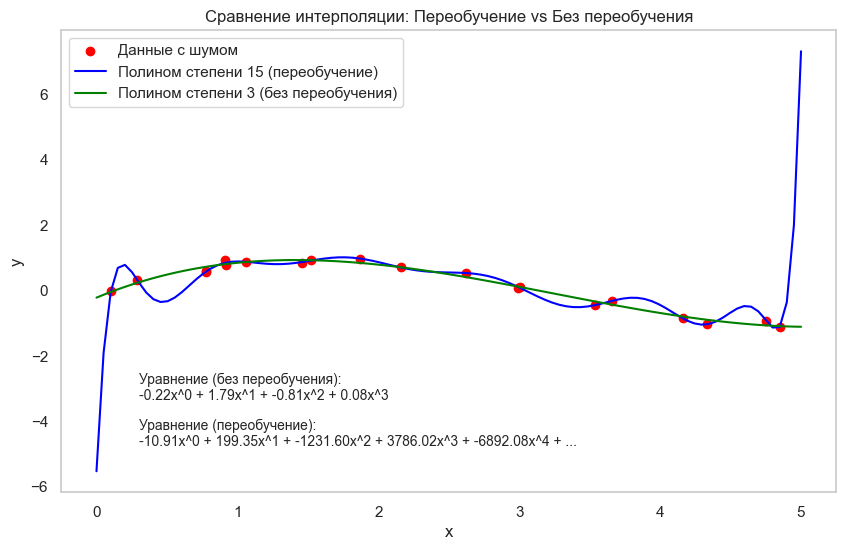
\includegraphics[width=0.9\linewidth]{chapters/linear/pics/reg-overfitting.png}
	\caption{Иллюстрация проблемы переобучения для решения линейной задачи}
	\label{linear-reg-overfitting}
\end{figure}

В разделе~\ref{linear-reg-l1l2} рассмотрены основные методы регуляризации, применяемые в линейных моделях. Раздел~\ref{linear-reg-prob} описывает вероятностную трактовку причин возникновения регуляризации. Завершается глава разделом~\ref{linear-reg-task}, который содержит три теоретических задачи по теме регрессии.

\subsection{Гауссовский и лапласовский регуляризаторы}
\label{linear-reg-l1l2}

Гауссовский и лапласовский регуляризаторы представляют собой две разные техники регуляризации, которые используются для управления сложностью моделей и предотвращения переобучения. Они основаны на различных подходах к штрафованию весов модели.

\subsubsection{Лапласовский регуляризатор (L1 регуляризатор)}

Лапласовский (L1) регуляризатор использует сумму модулей значений весов модели в качестве штрафа. Формально новую функцию потерь можно записать следующим образом:
$L1 = L_0 + \lambda \sum_{i=1}^{n} |w_i|$,
где $L_0$ --- исходная функция потерь, $|w_i|$ --- абсолютные значения весов модели, $\lambda$ --- коэффициент регуляризации.
\noindent
Преимущества:
\begin{itemize}
	\item Лапласовский регуляризатор может приводить к обнулению некоторых весов, что делает модель более интерпретируемой и позволяет выделять наиболее важные признаки.
	\item Он может быть особенно полезен в задачах с высокой размерностью, где много признаков могут быть неинформативными.
\end{itemize}
Недостатки:
\begin{itemize}
	\item Оптимизация с использованием L1 регуляризации может быть более сложной и требовать специальных алгоритмов (например, координатного спуска или методов, основанных на субградиенте).
\end{itemize}

\subsubsection{Гауссовский регуляризатор (L2 регуляризатор)}

Гауссовский (L2) регуляризатор использует штраф в виде суммы квадратов весов модели. Формально новую функцию потерь можно записать следующим образом:
$L2 = L_0 + \lambda \sum_{i=1}^{n} w_i^2$,
где $L_0$ — исходная функция потерь (например, среднеквадратичная ошибка для задачи регрессии), $w_i$ — веса модели, $\lambda$ — коэффициент регуляризации, который контролирует величину штрафа.
Преимущества:
\begin{itemize}
	\item Гауссовский регуляризатор помогает сгладить веса, что делает модель более устойчивой к шуму в данных.
	\item Он способствует распределению весов по всем признакам, уменьшая вероятность того, что некоторые признаки будут доминировать.
\end{itemize}
Недостатки:
\begin{itemize}
	\item Может не приводить к полному обнулению весов, поэтому не всегда приводит к интерпретируемым моделям.
\end{itemize}

\subsubsection {Сравнений L1 и L2 регуляризаторов}

Выбор между гауссовским и лапласовским регуляризаторами зависит от конкретной задачи и целей (сравнение см. в таблице~\ref{linear-reg-comp}). Если важна интерпретируемость модели и выделение значимых признаков, то стоит рассмотреть L1 регуляризацию. Если же цель — улучшить общее качество модели без сильного сокращения количества признаков, то L2 регуляризация может быть предпочтительнее. Это связано с тем, что в L2 регуляризации за счет возведения в квадрат значений весов вклад нулевого веса и просто малого веса неразличим на при наличии других выделенных признаков с весами порядка или более единицы. Таким образом, L2 регуляризация, в отличии от L1 не стремится обнулить коэффициенты, что снижает интерпретируемость модели. Однако квадратичная функция является гладкой, поэтому лучше поддается вычислительным методам оптимизации.

\begin{table}[h]
	\caption{Сравнение L1 и L2 регуляризаторов}
	\label{linear-reg-comp}
	\begin{tabular}{l|l|l}
		Характеристика & Лапласовский (L1) & Гауссовский (L2) \\
		\hline
		Штраф & Сумма абсолютных значений весов & Сумма квадратов весов \\
		Эффект на веса & Обнуление (спарсность) & Сглаживание \\
		Интерпретируемость & Выше & Меньше \\
		Оптимизация & Сложнее & Легче
	\end{tabular}
\end{table}

В ситуациях используется комбинация обоих методов регуляризации. Для этого вводится дополнительный гиперпараметр $\alpha$~--- доля первой нормы в штрафе за вес. Получается так называемая эластичная сеть (англ.: elastic net). В таком случае:
$L = L_0 + \lambda [\alpha \sum_{i=1}^{n} |w_i| + (1 - \alpha) \sum_{i=1}^{n} w_i^2]$. Данный подход позволяет учесть особенности двух подходов, однако усложняет модель.

\subsection {Вероятностная интерпретация регуляризации}
\label{linear-reg-prob}

В первом рассмотрении регуляризацию можно рассматриваться как введение априорной информации о параметрах модели. Рассмотрим вводимые предположения:
\begin{itemize}
	\item в случае L1 регуляризации мы предполагаем, что многие веса могут быть равны нулю, это соответствует идее о том, что истинная модель простая и присутствуют лишние признаки;
	\item в случае L2~--- веса распределены вблизи общего малого среднего значения, это отражает предположение о том, что все признаки вносят сопоставимый вклад в предсказание.
\end{itemize}
\noindent
Описанным выше предположениям о весах соответствуют экспоненциальное и нормальное распределения (см. рис.~\ref{linear-reg-distribution}). Рассмотрим их влияние на штраф и функцию потерь.

\begin{figure}[h]
	\centering
	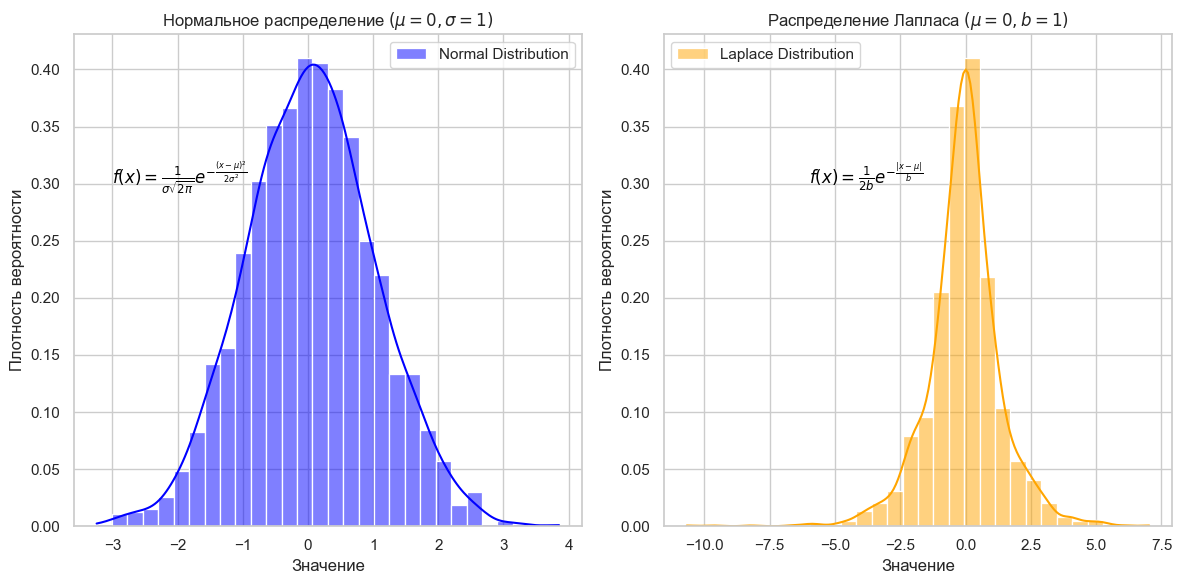
\includegraphics[width=0.9\linewidth]{chapters/linear/pics/reg-distributions.png}
	\caption{Сравнение экспоненциального и нормального распределений}
	\label{linear-reg-distribution}
\end{figure}

\subsubsection {L1 регуляризация}

предполагает, что веса $w_j$ распределены по лапласовскому закону (или двойному экспоненциальному распределению), $w_j - Laplace(0, b)$.

\subsubsection{L2 регуляризация} 

предполагает, что веса модели $w_j$ имеют нормальное распределение с нулевым средним и некоторой дисперсией $\sigma^2$. Это можно записать как $w_j - N(0, \sigma^2)$.

\subsection {Задачи}
\label{linear-reg-task}


\subsubsection{Вопрос 1}
\noindent Как изменение коэффициента $\lambda$ влияет на величину весов $w_j$?

\textbf{L1 регуляризация}

\noindent При увеличении $\lambda$ происходит обнулению некоторых весов $w_j$. Это приводит к тому, что с увеличением $\lambda$ количество ненулевых весов уменьшается, что может помочь в отборе признаков и упрощении модели.

\textbf{L2 регуляризация}

\noindent При увеличении $\lambda$ происходит увеличение штрафа за большие значения весов. Это приводит к уменьшению величины весов $w_j$ (все веса стремятся к нулю), что помогает избежать переобучения. В случае $\lambda$ = 0 модель не имеет регуляризации, и веса могут принимать любые значения, что может привести к переобучению.

\subsubsection{Вопрос 2}
\noindent Какова геометрическая интерпретация регуляризации в пространстве весов?

\begin{figure}[h]
	\centering
	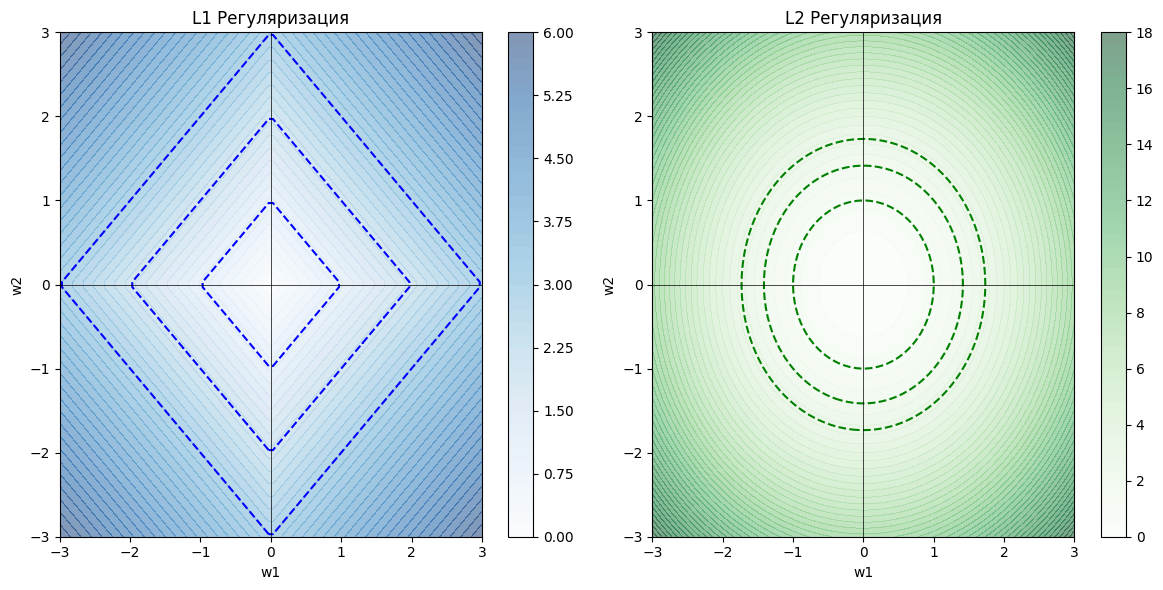
\includegraphics[width=0.9\linewidth]{chapters/linear/pics/reg-geom.png}
	\caption{Геометрическая интерпретация регуляризации в пространстве весов}
	\label{linear-reg-geom}
\end{figure}

\textbf{L1 регуляризация}

\noindent Геометрически L1 регуляризация создает ромбовидные (или параллелепипедные) области в пространстве весов. Оптимальные веса находятся на вершинах этих ромбов, что приводит к обнулению некоторых весов и, следовательно, к отбору признаков.

$L1(w_1,w_2) = const <=> |w_1|+|w_2| = const$

\textbf{L2 регуляризация}

\noindent Геометрически L2 регуляризация создает сферу (или гиперсферу) в пространстве весов, внутри которой минимизируется функция потерь. Это означает, что оптимальные веса будут находиться на поверхности этой сферы, что приводит к сглаживанию и уменьшению значений весов.

$L2(w_1,w_2) = const <=> w_1^2+w_2^2 = const$

\subsubsection{Вопрос 3}
\noindent Какие особенности признаков компенсируют регуляризации?

\textbf{L1 регуляризация}

\noindent Используя L1 регуляризацию, можно обнулить веса для менее значимых признаков. После обучения модели можно проанализировать ненулевые веса и оставить только те признаки, которые имеют значимые коэффициенты, тем самым осуществляя отбор признаков.

\textbf{L2 регуляризация}

\noindent L2 регуляризация помогает сгладить веса при наличии мультиколлинеарности, уменьшая их величину и тем самым снижая влияние коррелирующих признаков. Это позволяет избежать чрезмерного увеличения весов для сильно коррелирующих признаков.

\section*{Основная идея}

Градиентные методы --- это широкий класс оптимизационных алгоритмов, используемых не только в машинном обучении. Здесь градиентный подход будет рассмотрен в качестве способа подбора вектора синаптических весов \( w \) в линейном классификаторе. Пусть \( y^*: \, X \to Y \) — целевая зависимость, известная только на объектах обучающей выборки: \( X^l = (x_i, y_i)_{i=1}^l \), где \( y_i = y^*(x_i) \).

Найдём алгоритм \( a(x, w) \), аппроксимирующий зависимость \( y^* \). В случае линейного классификатора искомый алгоритм имеет вид:
$$ a(x, w) = \varphi\left(\sum_{j=1}^n w_j x^j - w_0\right), $$
где \( \varphi(z) \) играет роль функции активации (в простейшем случае можно положить \( \varphi(z) = \operatorname{sign}(z) \)).

Согласно принципу минимизации эмпирического риска, для этого достаточно решить оптимизационную задачу:
$$ Q(w) = \sum_{i=1}^l L(a(x_i, w), y_i) \to \min_w, $$
где \( L(a, y) \) — заданная функция потерь.

Для минимизации применим метод градиентного спуска (gradient descent). Это пошаговый алгоритм, на каждой итерации которого вектор \( w \) изменяется в направлении наибольшего убывания функционала \( Q \) (то есть в направлении антиградиента):
$$ w := w - \eta \nabla Q(w), $$
где \( \eta \) — положительный параметр, называемый темпом обучения (learning rate).

\subsection*{Основные подходы к реализации градиентного спуска}
\begin{enumerate}
    \item \textbf{Пакетный (batch):} на каждой итерации обучающая выборка просматривается целиком, и только после этого изменяется \( w \). Этот подход требует больших вычислительных затрат.
    \item \textbf{Стохастический (stochastic/online):} на каждой итерации из обучающей выборки случайным образом выбирается один объект. Таким образом, вектор \( w \) настраивается на каждый вновь выбираемый объект.
\end{enumerate}

\subsection*{Алгоритм Stochastic Gradient (SG)}
\textbf{Вход:}
\begin{itemize}
    \item \( X^l \) --- обучающая выборка;
    \item \( \eta \) --- темп обучения;
    \item \( \lambda \) --- параметр сглаживания функционала \( Q \).
\end{itemize}

\textbf{Выход:} Вектор весов \( w \)

\textbf{Тело алгоритма:}
\begin{enumerate}
    \item Инициализировать веса \( w_j \), \( j = 0, \dots, n \);
    \item Инициализировать текущую оценку функционала: \( Q := \sum_{i=1}^l L(a(x_i, w), y_i) \);
    \item Повторять:
    \begin{enumerate}
        \item выбрать объект \( x_i \) из \( X^l \) (например, случайным образом);
        \item вычислить выходное значение алгоритма \( a(x_i, w) \) и ошибку: \( \varepsilon_i := L(a(x_i, w), y_i) \);
        \item сделать шаг градиентного спуска:
        $$ w := w - \eta L_a^\prime (a(x_i, w), y_i) \varphi^\prime (\langle w, x_i \rangle)x_i; $$
        \item оценить значение функционала:
        $$ Q := (1 - \lambda)Q + \lambda\varepsilon_i; $$
    \end{enumerate}
    пока значение \( Q \) не стабилизируется и/или веса \( w \) не перестанут изменяться.
\end{enumerate}

\subsection*{Порядок выбора объектов}
В случае стохастического градиентного спуска объекты следует выбирать случайным образом, однако существуют эвристики, направленные на улучшение сходимости:
\begin{itemize}
    \item Перемешивание (shuffling): случайно выбирать объекты, попеременно из разных классов. Идея в том, что объекты из разных классов менее "похожи", чем объекты одного класса, поэтому вектор \( w \) будет сильнее изменяться.
    \item Можно выбирать объект с вероятностью, обратно пропорциональной величине ошибки на объекте. Следует учитывать, что такая эвристика делает метод чувствительным к шумам.
\end{itemize}

\subsection*{Способы инициализации весов}
\begin{enumerate}
    \item Инициализация вектора \( w \) нулями.
    \item \( w_j := \operatorname{rand}\left(-\frac{1}{n}, \frac{1}{n}\right) \), где \( n \) — размерность пространства признаков.
    \item Решение исходной оптимизационной задачи при условии статистически независимых признаков, линейной функции активации (\( \varphi \)) и квадратичной функции потерь (\( L \)):
    $$ w_j := \frac{\langle y, f_j \rangle}{\langle f_j, f_j \rangle}. $$
\end{enumerate}

\subsection*{Параметр сглаживания}
Для оценки функционала \( Q \) на каждой итерации используется его приближённое значение по методу экспоненциального сглаживания, откуда \( \lambda \) лучше брать порядка \( \frac{1}{l} \).

\subsection*{Известные частные случаи алгоритма}
Метод SG (при соответствующем выборе функций активации и потерь) является обобщением следующих эвристик подбора \( w \) и алгоритмов классификации:
\begin{itemize}
    \item Адаптивный линейный элемент (Adalines);
    \item Правило Хэбба;
    \item Алгоритм \( k \)-средних (K-Means);
    \item Learning Vector Quantization (LVQ).
\end{itemize}

\subsection*{Преимущества SG}
\begin{itemize}
    \item Метод подходит для динамического (online) обучения.
    \item Алгоритм способен обучаться на избыточно больших выборках.
    \item Различные стратегии обучения позволяют адаптировать алгоритм для задач с избыточной или небольшой выборкой.
\end{itemize}

\subsection*{Недостатки SG и способы их устранения}
\begin{itemize}
    \item Возможны проблемы сходимости. Для борьбы с этим применяют технику встряхивания коэффициентов.
    \item При высокой размерности пространства признаков \( n \) и/или малой длине выборки \( l \) возможно переобучение. Для борьбы с этим применяют метод сокращения весов:
    $$ Q_{\tau}(w) = Q(w) + \frac{\tau}{2}||w||^2. $$
    Тогда правило обновления весов принимает вид:
    $$ w := w(1 - \eta \tau) - \eta \nabla Q(w). $$
    \item При больших значениях \( \langle w, x_i \rangle \) значение \( \varphi^\prime \) может становиться близким к нулю. Для предотвращения этого состояния вводят нормализацию признаков:
    $$ x^j := \frac{x^j - x_{\min}^j}{x_{\max}^j - x_{\min}^j}, \quad j = 1, \dots, n, $$
    где \( x_{\min}^j, x_{\max}^j \) — минимальное и максимальное значения признака \( j \)-го признака. Регуляризация, такая как weight decay, также помогает избежать "паралича".
\end{itemize}

\subsection*{Сходимость алгоритма}
Сходимость гарантируется при выпуклой функции \( Q(w) \) и выполнении следующих условий:
$$ \eta_t \xrightarrow{t \to \infty} 0, \quad \sum_{t=1}^{\infty} \eta_t = \infty, \quad \sum_{t=1}^{\infty} \eta_t^2 < \infty. $$
Например, можно положить \( \eta_t = \frac{\eta_0}{t} \), хотя на практике это не всегда удачно.

\section*{Задачи}

\subsection*{Задача 1: Доказать сходимость алгоритма при условиях выше}

\textbf{Решение:}

\begin{enumerate}
    \item \textbf{Выпуклость функции:} Поскольку \( Q(w) \) выпукла, мы можем использовать свойства выпуклых функций. Для любого \( w \) и \( w^* \) (где \( w^* \) — точка минимума функции \( Q \)) выполняется неравенство:
    $$ Q(w) \geq Q(w^*) + \nabla Q(w^*)^T (w - w^*). $$

    \item \textbf{Итерация метода стохастического градиента:} Обновление весов в SGD задается следующим образом:
    $$ w_{t+1} = w_t - \eta_t \nabla Q(w_t; \xi_t), $$
    где \( \xi_t \) — случайная переменная, представляющая выборку данных на итерации \( t \).

    \item \textbf{Анализ изменения функции:} Мы можем оценить изменение функции \( Q \) на каждой итерации:
    $$ Q(w_{t+1}) \leq Q(w_t) + \nabla Q(w_t; \xi_t)^T (w_{t+1} - w_t) + \frac{L}{2} \|w_{t+1} - w_t\|^2, $$
    где \( L \) — константа Липшица для градиента \( \nabla Q \).

    Подставляя обновление:
    $$ Q(w_{t+1}) \leq Q(w_t) - \eta_t \nabla Q(w_t; \xi_t)^T \nabla Q(w_t) + \frac{L}{2} \eta_t^2 \|\nabla Q(w_t; \xi_t)\|^2. $$

    \item \textbf{Суммирование изменений:} Суммируя по всем итерациям, мы получаем:
    $$ \sum_{t=1}^{T} Q(w_{t+1}) - Q(w_1) \leq -\sum_{t=1}^{T} \eta_t \nabla Q(w_t; \xi_t)^T \nabla Q(w_t) + \sum_{t=1}^{T} \frac{L}{2} \eta_t^2 \|\nabla Q(w_t; \xi_t)\|^2. $$

    \item \textbf{Использование условий:} Условия \( \sum_{t=1}^{\infty} \eta_t = \infty \) и \( \sum_{t=1}^{\infty} \eta_t^2 < \infty \) позволяют нам сделать вывод о том, что:
    \begin{itemize}
        \item Сумма шагов обучения стремится к бесконечности, что означает, что веса \( w_t \) будут продолжать обновляться.
        \item Сумма квадратов шагов обучения конечна, что позволяет контролировать величину изменений на каждой итерации.
    \end{itemize}

    \item \textbf{Сходимость к минимуму:} В результате, при условии, что \( Q(w) \) выпукла, и учитывая условия на шаги обучения, мы можем утверждать, что последовательность \( w_t \) будет сходиться к некоторой точке \( w^* \), которая является минимумом функции \( Q(w) \).
\end{enumerate}

Таким образом, метод стохастического градиента сходится к минимуму выпуклой функции \( Q(w) \) при выполнении заданных условий.

\subsection*{Задача 2: Оценка вариации градиента}

\textbf{Условие:} Пусть \( \xi_1, \xi_2, \ldots, \xi_n \) — независимые и одинаково распределённые (i.i.d.) случайные переменные, представляющие собой выборки из обучающего набора. Рассмотрим стохастический градиент \( \nabla L(\theta; \xi_t) \).

\textbf{Задача:} Доказать, что математическое ожидание стохастического градиента совпадает с истинным градиентом функции потерь:
\[
\mathbb{E}[\nabla L(\theta; \xi_t)] = \nabla L(\theta)
\]
и оценить дисперсию \( \operatorname{Var}(\nabla L(\theta; \xi_t)) \) в зависимости от размера выборки \( n \).

\subsection*{Доказательство}

\begin{enumerate}
    \item \textbf{Определение стохастического градиента:} Пусть \( L(\theta) \) — функция потерь, зависящая от параметров \( \theta \) и от выборки \( \xi \). Мы можем записать функцию потерь как среднее значение по всем данным:
    $$ L(\theta) = \frac{1}{n} \sum_{i=1}^{n} l(\theta; x_i, y_i), $$
    где \( l(\theta; x_i, y_i) \) — функция потерь для примера \( (x_i, y_i) \).

    \item \textbf{Истинный градиент:} Тогда истинный градиент функции потерь можно выразить как:
    $$ \nabla L(\theta) = \frac{1}{n} \sum_{i=1}^{n} \nabla l(\theta; x_i, y_i). $$

    \item \textbf{Математическое ожидание стохастического градиента:} Теперь рассмотрим стохастический градиент:
    $$ \nabla L(\theta; \xi_t) = \nabla l(\theta; \xi_t), $$
    где \( \xi_t \) — случайная выборка. Поскольку \( \xi_t \) выбирается из одного из \( n \) примеров, математическое ожидание стохастического градиента будет:
    \[
    \mathbb{E}[\nabla L(\theta; \xi_t)] = \mathbb{E}[\nabla l(\theta; \xi_t)] = \frac{1}{n} \sum_{i=1}^{n} \nabla l(\theta; x_i, y_i) = \nabla L(\theta).
    \]
    Таким образом, мы доказали, что:
    \[
    \mathbb{E}[\nabla L(\theta; \xi_t)] = \nabla L(\theta).
    \]

    \item \textbf{Оценка дисперсии:} Теперь найдём дисперсию стохастического градиента:
    \[
    \operatorname{Var}(\nabla L(\theta; \xi_t)) = \mathbb{E}[(\nabla L(\theta; \xi_t) - \mathbb{E}[\nabla L(\theta; \xi_t)])^2].
    \]
    Подставим выражение для стохастического градиента:
    \[
    \operatorname{Var}(\nabla L(\theta; \xi_t)) = \mathbb{E}[(\nabla l(\theta; \xi_t) - \nabla L(\theta))^2].
    \]
    Поскольку \( \xi_t \) является случайным выбором, мы можем использовать свойства дисперсии. Для \( n \) независимых и одинаково распределённых (i.i.d.) выборок дисперсия стохастического градиента будет уменьшаться с увеличением размера выборки:
    $$ \operatorname{Var}(\nabla L(\theta; \xi_t)) = \frac{1}{n} \operatorname{Var}(l(\theta; x, y)), $$
    где \( (x, y) \) — случайная выборка из обучающего набора. Это означает, что дисперсия стохастического градиента уменьшается с увеличением размера выборки \( n \).
\end{enumerate}

\subsection*{Задача 3: Регуляризация и стохастический градиент}

\subsection*{Условие}
Рассмотрим функцию потерь с L2-регуляризацией:
$$ L(\theta) = \frac{1}{n} \sum_{i=1}^{n} l(\theta; x_i, y_i) + \frac{\lambda}{2} \|\theta\|^2 $$
где \( l(\theta; x_i, y_i) \) — функция потерь для примера \( (x_i, y_i) \), а \( \lambda \) — коэффициент регуляризации.

\subsection*{Задача}
Обосновать, как регуляризация влияет на сходимость метода стохастического градиента, и показать, что использование регуляризации может помочь избежать переобучения, уменьшая значение функции потерь на валидационном наборе.

\subsection*{Влияние регуляризации на сходимость метода стохастического градиента}
\begin{enumerate}
    \item \textbf{Сглаживание функции потерь:}
    \begin{itemize}
        \item Добавление L2-регуляризации к функции потерь делает её более гладкой и выпуклой. Это связано с тем, что регуляризационный член \( \frac{\lambda}{2} \|\theta\|^2 \) добавляет "наказание" за большие значения параметров, что предотвращает резкие изменения градиента.
        \item Гладкость функции потерь способствует более стабильному обновлению параметров при использовании стохастического градиента. Это означает, что обновления параметров будут более предсказуемыми и менее подвержены шуму, что улучшает сходимость алгоритма.
    \end{itemize}

    \item \textbf{Уменьшение переобучения:}
    \begin{itemize}
        \item Регуляризация способствует уменьшению значений параметров модели, что, в свою очередь, снижает сложность модели. Это позволяет избежать переобучения, когда модель слишком точно подстраивается под тренировочные данные, включая шум.
        \item В результате, при использовании регуляризации, модель будет лучше обобщаться на новых данных, что выражается в меньшем значении функции потерь на валидационном наборе.
    \end{itemize}
\end{enumerate}

\subsection*{Доказательство эффекта регуляризации на валидационном наборе}
\begin{enumerate}
    \item \textbf{Функция потерь на валидационном наборе:}
    \begin{itemize}
        \item Пусть \( L_{val}(\theta) \) — функция потерь на валидационном наборе. При использовании регуляризации, мы можем записать:
        $$ L_{val}(\theta) = \frac{1}{m} \sum_{j=1}^{m} l(\theta; x_j, y_j) + \frac{\lambda}{2} \|\theta\|^2 $$
        где \( m \) — количество примеров в валидационном наборе.
    \end{itemize}

    \item \textbf{Сравнение значений функции потерь:}
    \begin{itemize}
        \item Без регуляризации, модель может иметь высокую функцию потерь на валидационном наборе из-за переобучения. При добавлении L2-регуляризации, даже если функция потерь на тренировочном наборе остаётся низкой, регуляризация помогает поддерживать значение функции потерь на валидационном наборе на более низком уровне.
    \end{itemize}

    \item \textbf{Кросс-валидация для выбора \( \lambda \):}
    \begin{itemize}
        \item Оптимальное значение \( \lambda \) можно выбрать с помощью кросс-валидации. Это позволяет находить компромисс между сложностью модели и её обобщающей способностью, что в конечном итоге приводит к меньшему значению функции потерь на валидационном наборе.
    \end{itemize}
\end{enumerate}

\subsection*{Заключение по задаче 3}
Регуляризация, особенно L2-регуляризация, играет ключевую роль в улучшении сходимости метода стохастического градиента и в предотвращении переобучения модели. Она помогает сделать функцию потерь более гладкой и выпуклой, что способствует стабильности обновлений параметров. В результате, использование регуляризации приводит к лучшему обобщению модели и снижению значения функции потерь на валидационном наборе, что является важным аспектом при разработке надёжных моделей в машинном обучении.

\newpage

\section{Метод наименьших квадратов (МНК) в общем случае}

\subsection{Про линейную регрессию и МНК}

Линейная регрессия — это метод анализа данных, который используется для определения линейной зависимости между зависимой переменной \(y\) и одной или несколькими независимыми переменными \(x_1, x_2, \dots, x_n\). Цель метода заключается в построении модели, которая минимизирует ошибку предсказания.  

Метод наименьших квадратов (МНК) — это наиболее распространённый способ нахождения коэффициентов линейной регрессии. Он минимизирует сумму квадратов отклонений предсказанных значений от наблюдаемых. Таким образом, МНК позволяет определить такие коэффициенты \( \beta_0, \beta_1, \dots, \beta_n \), которые обеспечивают наилучшее соответствие модели данным.  

\textbf{Основная идея МНК:} минимизация ошибки предсказания, заданной формулой:
\[
Q(\beta) = \sum_{i=1}^{N} (y_i - \hat{y_i})^2,
\]
где \(y_i\) — наблюдаемые значения, а \( \hat{y_i} \) — предсказанные моделью значения.

\subsection{МНК в общем случае}

\textbf{\textit{Определение:}}  
В общем случае задача линейной регрессии может быть представлена в матричной форме:
\[
\mathbf{y} = X \beta + \epsilon,
\]
где:  
- \(y\) — вектор целевых значений (\(N \times 1\)), \\
- \(X\) — матрица признаков (\(N \times p\)), \\
- \(\beta\) — вектор коэффициентов модели (\(p \times 1\)), \\
- \(\epsilon\) — вектор ошибок (\(N \times 1\)).  

Решение задачи МНК определяется как:
\[
\hat{\beta} = (X^T X)^{-1} X^T \mathbf{y}.
\]

\textbf{\textit{Интерпретация:}}  
Этот результат минимизирует сумму квадратов остатков \(\epsilon = \mathbf{y} - X\beta\). В случае, если матрица \(X^T X\) вырожденная, решение может быть некорректным или недоступным, что требует применения регуляризации.

\subsection{Проблемы и ограничения МНК}

Несмотря на простоту и эффективность, метод МНК имеет ограничения:  

\begin{enumerate}

    \item \textbf{Мультиколлинеарность}
		\begin{itemize}
			\item \textbf{Определение:} мультиколлинеарность возникает, когда между независимыми переменными в матрице признаков X существует сильная линейная зависимость;
			\item \textbf{Почему это проблема:} при мультиколлинеарности матрица \(X^T X\) становится плохо обусловленной (или даже вырожденной), что затрудняет нахождение её обратной матрицы. Это может привести к неустойчивым решениям, при которых малые изменения в данных существенно изменяют значения коэффициентов.
		\end{itemize}

	\item \textbf{Чувствительность к выбросам}
		\begin{itemize}
			\item \textbf{Определение:} МНК минимизирует сумму квадратов ошибок, что делает его очень чувствительным к выбросам (аномальным точкам);
			\item \textbf{Почему это проблема:} выбросы имеют большое влияние на значение целевой функции \(Q(\beta)\), что может привести к сильному смещению коэффициентов регрессии.
		\end{itemize}

	\item \textbf{Нарушение предположений:} МНК предполагает линейность модели, гомоскедастичность (постоянную дисперсию ошибок) и отсутствие автокорреляции.
	
	\item \textbf{Высокая вычислительная сложность}
		\begin{itemize}
			\item \textbf{Определение:} МНК требует вычисления матрицы \(X^T X\) и её обратной, что имеет временную сложность \(O(Np^2+p^3)O(Np^2+p^3)\), где N — количество наблюдений, p — количество признаков;
			\item \textbf{Почему это проблема:} для больших наборов данных с большим количеством признаков вычислительная сложность становится значительной, что может сделать процесс обучения долгим.
		\end{itemize}
		
\end{enumerate}

\subsection{Задачи}

\textbf{Задача 1:}
Докажите, что решение системы нормальных уравнений для метода наименьших квадратов существует и единственно, если матрица \(X^T X\) положительно определённая. \\
\textbf{Решение:}
Метод наименьших квадратов минимизирует квадратичную функцию:
\[
Q(\beta) = \|y - X\beta\|^2 = (y - X\beta)^T (y - X\beta)
\]
Рассмотрим стационарные точки функции \(Q(\beta)\), задаваемые системой нормальных уравнений:
\[
X^TX\beta = X^Ty
\]
- Условие существования решения: \\
Решение существует, если матрица \(X^T X\) невырожденная, то есть её детерминант \(\det(X^T X) \neq 0\). Это выполняется, если признаки в X линейно независимы (нет мультиколлинеарности). \\
- Условие единственности решения: \\
Если \(X^T X\) положительно определённая, то:  
\begin{enumerate}
	\item \((X^T X)\) симметрична.
	\item Для любого ненулевого вектора \(v\), \(v^T(X^T X)v > 0\).
\end{enumerate}
Положительная определённость гарантирует, что квадратичная форма \(Q(\beta)\) строго выпуклая, а значит, имеет единственную точку минимума.

\textbf{Задача 2:}
Опишите, как изменится целевая функция метода наименьших квадратов \( Q(\beta) = \|y - X\beta\|^2 \), если в данных присутствует выброс. Почему минимизация квадратичной ошибки делает метод чувствительным к таким точкам? \\
\textbf{Решение:}
Выбросы увеличивают квадратичную ошибку, так как вклад отклонений от линии регрессии для таких точек пропорционален квадрату расстояния. Это означает, что несколько больших ошибок могут доминировать над множеством малых, и решение будет смещено в сторону выбросов. Например, если одна ошибка вдвое больше остальных, её вклад в целевую функцию будет в четыре раза больше. Это делает МНК очень чувствительным к выбросам и может привести к неверным коэффициентам модели.  

\textbf{Задача 3:}  
Реализуйте простой случай МНК для одномерной линейной регрессии, где \(X = [1, 2, 3]\), \(y = [2, 4, 6]\). Найдите коэффициенты \(\beta_0\) и \(\beta_1\). \\
\textbf{Решение:}
Для одномерного случая формула нормальных уравнений имеет вид:
\[
\hat{\beta} = (X^T X)^{-1} X^T y.
\]
Подставляя значения:
\[
X = \begin{bmatrix}
1 & 1 \\
1 & 2 \\
1 & 3
\end{bmatrix}, \quad y = \begin{bmatrix} 2 \\ 4 \\ 6 \end{bmatrix}.
\]
Рассчитаем:
\[
X^T X = \begin{bmatrix}
3 & 6 \\
6 & 14
\end{bmatrix}, \quad X^T y = \begin{bmatrix}
12 \\
28
\end{bmatrix}.
\]
Получаем:
\[
\hat{\beta} = \begin{bmatrix}
3 & 6 \\
6 & 14
\end{bmatrix}^{-1} \begin{bmatrix}
12 \\
28
\end{bmatrix}.
\]
После вычислений \(\hat{\beta} = \begin{bmatrix} 0 \\ 2 \end{bmatrix}\). Таким образом, уравнение линейной регрессии: \(y = 2x\).

\newpage

\section{Вероятностные функции потерь}

\subsection{Принцип максимума правдоподобия}

Предположим, что \(X\times Y\) - \textbf{вероятностное пространство} с некоторой \textbf{плотностью совместного распределения} пары объект-ответ \(p(x,y)\). 
Пусть \(X^{l}\) - \textit{простая} (i.i.d., или independent identically distributed - независимо из одного и того же распределения) выборка: \({(x_{i}, y_{i})^{l}}\), порожденная \(p(x,y)\). 

Задача состоит в том, чтобы оценить по выборке \(X^{l}\) плотность распределения \(p(x,y)\). Получив оценку плотности, то с его помощью возможна классификация объекта \(x\) - мы сможем вычислять вероятность класса \(y\) для любого объекта \(x\). 

Далее введем \textbf{параметризацию} плотности, взяв за основу формулу условной вероятности: \(p(x,y) = P(y | x,w)p(x)\), где \(p(x,y)\) - искомая плотность; \(P(y|x,w\) - модель условной вероятности класса с параметром \(w\); \(p(x)\) - непараметризуемое распределение в пространстве \(X\). Возможны и другие способы введения параметризации, однако сейчас будет рассматриваться именно этот.

Так как выборка простая, то плотность порожденной выборки является произведением плотностей отдельных порожденных пар \((x_{i}, y_{i})\). Таким образом, \(\prod_{i=1}^{l}{p(x_{i},y_{i})}\) - \textit{правдоподобие данных}.

В качестве критерия оптимизации возьмем один из фундаментальных методов в математической статистике - \textbf{принцип максимума правдоподобия}:

\[
\prod_{i=1}^{l}{p(x_{i},y_{i})} = \prod_{i=1}^{l}{P(y_{i}|x_{i},w)p(x_{i})} \xrightarrow{} \max_{w} 
\]

В силу того, что \(p(x_{i})\) - сомножитель, не зависящий от \(w\), от него можно избавиться.

\[
\prod_{i=1}^{l}{P(y_{i}|x_{i},w)} \xrightarrow{} \max_{w} 
\]

Поскольку стоит задача максимизации, критерий в виде произведения по всем объектам выборки неудобен. Чтобы избавиться от произведения, прологарифмируем критерий. Логарифм - монотонная функция, поэтому несущественно, что мы оптимизируем - функционал или его логарифм.

\textbf{Логарифм правдоподобия} (log-likehood, log-loss):

\[
L(w) = \sum_{i=1}^{l}{log \ P(y_{i}|x_{i},w)} \xrightarrow{} \max_{w}
\]

\subsection{Связь правдоподобия и аппроксимации эмпирического риска}

Посмотрим на одну и ту же задачу классификации на два класса \(Y = \{+1; -1\}\) с двух сторон:
\begin{enumerate}
    \item \(P(y|x,w)\) - вероятностная модель классификации. 
    \item \(g(x,w)\) - разделяющая (дискриминантная) функция - геометрический взгляд на задачу.
\end{enumerate}

Критерии, возникающие в разных случаях:
\begin{enumerate}

    \item \textit{Максимизация правдоподобия} (Maximum Likehood): 
    \[
    L(w) = \sum_{i=1}^{l}{log \ P(y_{i}|x_{i},w)} \xrightarrow{} \max_{w};
    \]
    
    \item \textit{Минимизация аппроксимированного эмпирического риска}:
    \[
    Q(w) = \sum_{i=1}^{l}{L(y_{i}g(x_{i},w))} \xrightarrow{} \min_{w};
    \]
    Здесь \(L(M)\) - функция потерь; \(y_{i}g(x_{i}, w)\) - значение отступa.

\end{enumerate}


Оба критерия представляют собой оптимизацию некоторой величины, являющейся суммой по всем объектам выборки, по параметру. Каждое слагаемое суммы зависит только от одного объекта. 

Эти два принципа \textbf{эквиваленты}, если положить:

\[
-log \ P(y_{i}|x_{i},w) = L(y_{i}g(x_{i},w)
\]

\subsection{Вероятностный смысл регуляризации}

Рассматривается двухуровневая модель порождения данных:
\begin{enumerate}
    \item \(P(y|x,w\) - вероятностная модель данных.
    \item \(p(w;y)\) - априорное распределение параметров модели.
    \item \(\gamma\) - вектор гиперпараметров.
\end{enumerate}

Теперь не только появление выборки \(X^{l}\), но и модели \(w\) полагается стохастическим. 

Совместное правдоподобие данных и модели по формуле условной плотности:

\[
p(X^{l},w) = p(X^{l}|w)p(w;\gamma)
\]

\textit{Принцип максимума апостериорной вероятности} (Maximum a Posteriori Probability, MAP):

\[
L(w) = log \ p(X^{l},w) = \sum_{i=1}^{l}{log \ P(y_{i}|x_{i},w) + log \ p(w;\gamma)} \xrightarrow{} \max_{w}
\]

Таким образом, слагаемое \(-log \ p(w;\gamma)\) является \textbf{регуляризатором} с вероятностной точки зрения.

\subsection{Задачи}

\subsubsection{Задача 1.}
Какому регуляризатору соответствует апостериорное распределение параметров модели, имеющее вид распределения Гаусса?

\textit{Решение:}

Веса \(w_{j}\) независимы, \(E[w_{j}]=0\), \(D[w_{j}]=C\).

\[
p(w;C) = \frac{1}{{(2\pi C)}^{\frac{n}{2}}}exp(-\frac{||w^2||}{2C}), ||w^2||=\sum_{j=1}^{n}{w_{j}^2}
\]

\[
-ln \ p(w;C)=\frac{1}{2C}||w^2|| + const
\]

От константы можно избавиться:

\[
-ln \ p(w;C)=\frac{1}{2C}||w^2||
\]

Получаем квадратичный \((L_{2})\) регуляризатор. \(C\) является гиперпараметром, \(\tau = \frac{1}{C}\) - коэффициент регуляризации.

\subsubsection{Задача 2.}
Какому виду регуляризации соответствует апостериорное распределение параметров модели, имеющее вид распределения Лапласа?

\textit{Решение:}

Веса \(w_{j}\) независимы, \(E[w_{j}]=0\), \(D[w_{j}]=C\).

\[
p(w;C) = \frac{1}{{(2C)}^{n}}exp(-\frac{||w||}{C}), ||w||=\sum_{j=1}^{n}{|w_{j}|}
\]

\[
-ln \ p(w;C)=\frac{1}{C}||w|| + const
\]

От константы можно избавиться:

\[
-ln \ p(w;C)=\frac{1}{C}||w||
\]

Получаем абсолютный \((L_{1})\) регуляризатор. \(C\) является гиперпараметром, \(\tau = \frac{1}{C}\) - коэффициент регуляризации.

\subsubsection{Задача 3.}
Найти вид апостериорного распределения параметров модели, соответствующий регуляризатору Elastic Net:

\[
R(w;C_{1};C_{2}) = \frac{1}{C_{1}}\sum_{i=1}^{l}{|w_{i}|} + \frac{1}{2C_{2}}\sum_{i=1}^{l}{w_{i}^{2}}
\]

\textit{Решение:}

\[
-ln \ p(w;C_{1};C_{2}) = \frac{1}{C_{1}}||w|| + \frac{1}{2C_{2}}||w^2||
\]

С точностью до умножения на константу, получим:

\[
p(w;C_{1};C_{2}) = exp(-\frac{||w||}{C_{1}})exp(-\frac{||w^2||}{2C_{2}})
\]

\[
p(w;C_{1};C_{2}) = exp(-\frac{||w||}{C_{1}}-\frac{||w^2||}{2C_{2}})
\]


\section{Методы оценки и проверки моделей}

Оценка и проверка моделей являются важными этапами в построении машинного обучения. Эти методы позволяют определить, насколько хорошо модель обучается на данных и обобщает свои выводы на новых, ранее невиданных данных. Ниже представлены основные подходы к оценке и проверке моделей.

\subsection*{Кросс-валидация}
Кросс-валидация --- это метод проверки модели, который заключается в разбиении данных на несколько подвыборок (folds). Основные виды кросс-валидации:
\begin{itemize}
    \item \textbf{K-блочная кросс-валидация} (K-fold cross-validation): данные делятся на $K$ частей, и обучение проводится на $K-1$ частях, а тестирование на оставшейся части. Процесс повторяется $K$ раз, чтобы каждая часть данных использовалась для тестирования.
    \item \textbf{Leave-One-Out (LOO)}: частный случай кросс-валидации, где тестовая выборка состоит из одного наблюдения, а оставшиеся используются для обучения. Этот метод особенно полезен для небольших наборов данных, но может быть вычислительно затратным.
    \item \textbf{Stratified K-fold}: разновидность K-блочной кросс-валидации, где сохраняются пропорции классов в каждой из выборок, что особенно важно для несбалансированных данных.
\end{itemize}

Кросс-валидация помогает уменьшить риск переобучения и получить более надежные оценки качества модели.

\subsection*{Метрики качества}
Для оценки модели применяются различные метрики, выбор которых зависит от задачи (регрессия или классификация):
\begin{itemize}
    \item \textbf{Для регрессии:}
    \begin{itemize}
        \item Среднеквадратичная ошибка (MSE):
        \[
        \text{MSE} = \frac{1}{n} \sum_{i=1}^n (y_i - \hat{y}_i)^2.
        \]
        Эта метрика чувствительна к выбросам, так как большие ошибки квадратично увеличивают значение MSE.
        \item Средняя абсолютная ошибка (MAE):
        \[
        \text{MAE} = \frac{1}{n} \sum_{i=1}^n |y_i - \hat{y}_i|.
        \]
        MAE более устойчива к выбросам, так как ошибки учитываются линейно.
        \item Коэффициент детерминации ($R^2$):
        \[
        R^2 = 1 - \frac{\sum_{i=1}^n (y_i - \hat{y}_i)^2}{\sum_{i=1}^n (y_i - \bar{y})^2}.
        \]
        Значение $R^2$ показывает, какую долю дисперсии целевой переменной объясняет модель.
    \end{itemize}
    \item \textbf{Для классификации:}
    \begin{itemize}
        \item Точность (Accuracy):
        \[
        \text{Accuracy} = \frac{\text{Количество верных предсказаний}}{\text{Общее количество наблюдений}}.
        \]
        Используется для сбалансированных данных.
        \item Precision, Recall и $F_1$-мера:
        \[
        \text{Precision} = \frac{TP}{TP + FP}, \quad \text{Recall} = \frac{TP}{TP + FN}, \quad F_1 = 2 \cdot \frac{\text{Precision} \cdot \text{Recall}}{\text{Precision} + \text{Recall}}.
        \]
        Эти метрики особенно важны для несбалансированных классов.
        \item ROC-кривые и площадь под кривой (AUC):
        ROC-кривая показывает соотношение TPR (True Positive Rate) и FPR (False Positive Rate) при различных порогах классификации, а AUC характеризует общую способность модели различать классы.
    \end{itemize}
\end{itemize}

\subsection*{Разделение данных}
Одним из простейших методов проверки модели является разделение данных на обучающую и тестовую выборки. Чаще всего используется пропорция 70\%/30\% или 80\%/20\%. Однако этот метод имеет недостаток: если данные случайно разделены неудачно, это может привести к неверным оценкам качества модели.

Для улучшения оценки часто используется тройное разбиение данных:
\begin{itemize}
    \item \textbf{Обучающая выборка} (Train set): используется для обучения модели.
    \item \textbf{Валидационная выборка} (Validation set): используется для подбора гиперпараметров и предотвращения переобучения.
    \item \textbf{Тестовая выборка} (Test set): применяется для окончательной оценки модели.
\end{itemize}

\subsection*{Проблемы и рекомендации}
\begin{itemize}
    \item \textbf{Переобучение:} Если модель слишком сложная, она может хорошо работать на обучающих данных, но плохо обобщаться на тестовые. Регуляризация и кросс-валидация помогают бороться с этой проблемой.
    \item \textbf{Недообучение:} Слишком простые модели могут не учитывать важные зависимости в данных. Следует выбирать более сложные модели или добавлять новые признаки.
    \item \textbf{Сбалансированность данных:} Для несбалансированных данных рекомендуется использовать метрики, такие как Precision, Recall или AUC.
\end{itemize}

\section*{Задачи}

\begin{enumerate}
    \item Для датасета (сгенерируйте сами) с 10 000 объектов примените 5-блочную кросс-валидацию. Опишите, как будут разделены данные на обучающие и тестовые выборки на каждом шаге. Рассчитайте среднее значение метрики Accuracy, если на каждом шаге она принимает значения: 0.85, 0.87, 0.86, 0.84, 0.88.

    \item Для задачи регрессии выберите подходящую метрику качества из MSE, MAE или $R^2$ и объясните, почему вы сделали такой выбор. Рассчитайте её значение для предсказаний $\hat{y} = [3, 5, 2, 7]$ и истинных значений $y = [3, 5, 4, 6]$.

    \item В задаче классификации модель предсказала 100 объектов, из которых 70 были классифицированы правильно, 20 --- ложно положительными, а 10 --- ложно отрицательными. Рассчитайте Precision, Recall и $F_1$-меру.
\end{enumerate}

    \clearpage
    \chapter{Основы нейросетевых моделей}
    \section{Полносвязная нейронная сеть (Персептрон).}

\subsection{Модель нейрона МакКаллока-Питтса}

Рассмотрим модель нейрона МакКаллока-Питтса (1943) \cite{ModelMcCullochPitts}. Множество объектов $X$ (количество элементов множества $M$), множество ответов $Y$ (количество элементов множества $H_L$). Признаки объектов задаются вектором функций $\overrightarrow{f(x)} = [f_1(x), f_2(x), \dots, f_n(x)]^T$ таких, что $f_j: X \rightarrow \mathbb{R}$. Для объекта $x_m \in X$ с помощью этих функций определяется вектор вещественных признаков $\overrightarrow{x_m} = [x_m^1, x_m^2, \dots, x_m^n]^T$, где $x_m^j = f_j (x_m)$. Нейрон вычисляет функцию активации $\sigma$ от линейной комбинации вектора признаков $\overrightarrow{x_m}$ с весами $\overrightarrow{w}$. То есть выход нейрона $a(\overrightarrow{x_m}, \overrightarrow{w})$ вычисляется по формуле:
$$
a(\overrightarrow{x_m}, \overrightarrow{w}) = \sigma(\sum_{i = 1}^{n} x_m^i w_i - w_0) = \sigma (<\overrightarrow{x_m}, \overrightarrow{w}>)
$$
Математическая модель нейрона изображена на рисунке \ref{img:McCullochPittsModel}. Функцией активации $\sigma$ может быть любая непрерывная нелинейная функция. Нелинейность функции нужна, чтобы иметь возможность приблизить любую непрерывную функцию с желаемой точностью (теорема Горбаня, 1998). В формуле вектор признаков $\overrightarrow{x_m}$ дополнен элементом $-1$, который имеет вес $w_0$, что соответствует физической интерпретации нейрона. Нейрон $m$ получает на вход множество электрических сигналов $x_m^i$ по дендритам $i$. Каждый дендрит $i$ имеет свою толщину, и соответственно проводимость $w_i$. Чем выше проводимость $w_i$, тем больший вклад сигнала с данного дендрита в общую сумму. Нейрон суммирует сигналы с дендритов и если сумма выше порогового значения $w_0$, то он передаёт информацию дальше по аксону. Сигнал на выходе нейрона, то есть аксоне, определяется функцией активации $\sigma$.

\begin{figure}[h]
	\centering
	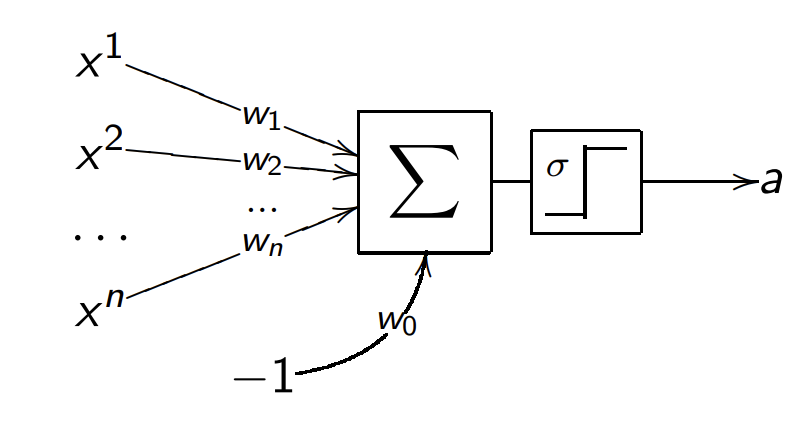
\includegraphics[width=0.4\linewidth]{chapters/neural/images/neuron1.png}
	\caption{Математическое описание модели нейрона МакКаллока-Питтса.}
	\label{img:McCullochPittsModel}
\end{figure}

\subsection{Реализация логических функций с помощью нейрона}

Рассмотрим применение описанного выше нейрона для реализации простейших логических функций.

\textbf{Логическая функция <<и>>}. Обозначение $\wedge$. На вход поступают признаки $x^1, x^2$, результат функции $a = x^1 \wedge x^2$. Нейронной реализацией будет $a = [x^1 + x^2 - \frac{3}{2} > 0]$, где функция активации $[x > 0]$ равна 1, если $x > 0$, и равна 0 в противном случае.

\begin{figure}[h]
	\centering
	\subfloat[Таблица истинности функции <<и>>]{
		\centering
		\begin{tabular}{|c|c|c|}
			\hline
			$x^1$ & $x^2$ & $a = x^1 \wedge x^2$ \\
			\hline
			0 & 0 & 0 \\
			0 & 1 & 0 \\
			1 & 0 & 0 \\
			1 & 1 & 1 \\
			\hline
		\end{tabular}
	}
	\hfill
	\subfloat[Модель нейрона, описывающего функцию <<и>>]{
		\centering
		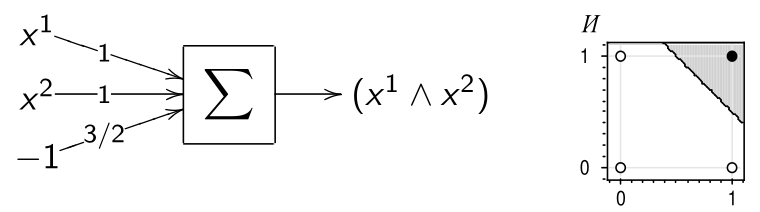
\includegraphics[width=0.45\linewidth]{chapters/neural/images/function_and.png}
	}
\end{figure}

\textbf{Логическая функция <<или>>}. Обозначение $\vee$. На вход поступают признаки $x^1, x^2$, результат функции $a = x^1 \vee x^2$. Нейронной реализацией будет $a = [x^1 + x^2 - \frac{1}{2} > 0]$, где функция активации $[x > 0]$ равна 1, если $x > 0$, и равна 0 в противном случае.

\begin{figure}[h]
	\centering
	\subfloat[Таблица истинности функции <<или>>]{
		\centering
		\begin{tabular}{|c|c|c|}
			\hline
			$x^1$ & $x^2$ & $a = x^1 \vee x^2$ \\
			\hline
			0 & 0 & 0 \\
			0 & 1 & 1 \\
			1 & 0 & 1 \\
			1 & 1 & 1 \\
			\hline
		\end{tabular}
	}
	\hfill
	\subfloat[Модель нейрона, описывающего функцию <<или>>]{
		\centering
		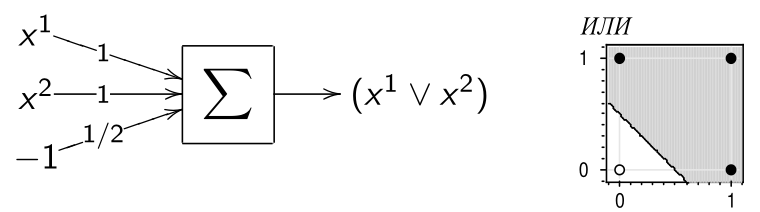
\includegraphics[width=0.45\linewidth]{chapters/neural/images/function_or.png}
	}
\end{figure}

\textbf{Задача 1.} Привести модель нейрона, описывающего логическую функцию <<не>> $\neg x^1$.

\textbf{Решение:}

$a = [-x^1 + 1/2 > 0]$

\newpage

\textbf{Логическая функция <<исключающее или>>}. Обозначение $\oplus$. Данная функция не реализуема с помощью одного нейрона. Но может быть реализована нейронной сетью $[n_1, n_2, n_3]$: $n_1 = (x^1 \vee x^2)$, $n_2 = (x^1 \wedge x^2)$, $n_3 = [n_1 - n_2 - \frac{1}{2} > 0]$.

\begin{figure}[h]
	\centering
	\subfloat[Таблица истинности функции <<исключающее или>>]{
		\centering
		\begin{tabular}{|c|c|c|}
			\hline
			$x^1$ & $x^2$ & $a = x^1 \oplus x^2$ \\
			\hline
			0 & 0 & 0 \\
			0 & 1 & 1 \\
			1 & 0 & 1 \\
			1 & 1 & 0 \\
			\hline
		\end{tabular}
	}
	\hfill
	\subfloat[Модель нейрона, описывающего функцию <<исключающее или>>]{
		\centering
		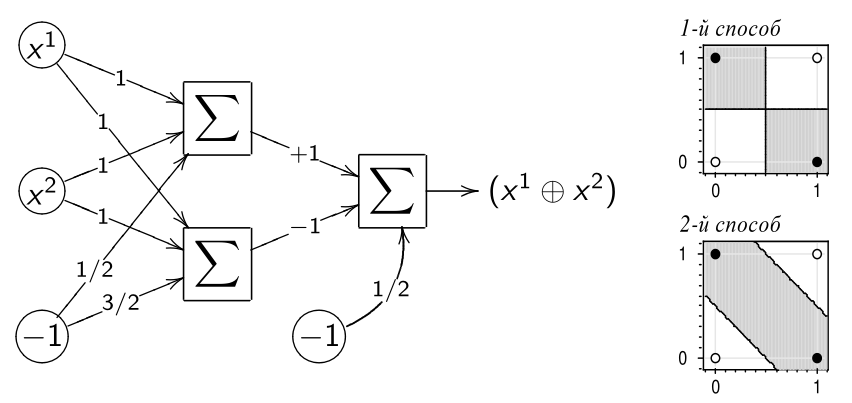
\includegraphics[width=0.45\linewidth]{chapters/neural/images/function_xor.png}
	}
\end{figure}

\textbf{Задача 2.} Привести модель нейронной сети, описывающей логическую функцию $f(x^1, x^2, x^3)$, заданную таблицей истинности: \\
\begin{figure}[h]
	\centering
	\begin{tabular}{|c|c|c|c|}
		\hline
		$x^1$ & $x^2$ & $x^3$ & $f(x^1, x^2, x^3)$ \\
		\hline
		0 & 0 & 0 & 0 \\
		0 & 0 & 1 & 1 \\
		0 & 1 & 0 & 0 \\
		0 & 1 & 1 & 0 \\
		
		1 & 0 & 0 & 1 \\
		1 & 0 & 1 & 1 \\
		1 & 1 & 0 & 0 \\
		1 & 1 & 1 & 1 \\
		\hline
	\end{tabular}
\end{figure}

\textbf{Решение:}

Используем ранее описанные нейроны <<и>> $\wedge$, <<или>> $\vee$, <<не>> $\neg$. Перепишем функцию, используя эти операции: $f = ((\neg x^1) \wedge ((\neg x^2) \wedge x^3)) \vee (x^1 \wedge ((\neg x^2) \vee x^3))$. Конструируем нейроны: $n_1 = \neg x^1$, $n_2 = \neg x^2$, $n_3 = n_2 \wedge x^3$, $n_4 = n_1 \wedge n_3$, $n_5 = n_2 \vee x^3$, $n_6 = x^1 \wedge n_5$, $n_7 = n_4 \vee n_6$. Итоговая многослойная нейронная сеть состоит из нейронов $n_1, n_2, \dots n_7$. Результат сети находится на выходе нейрона $n_7$.

\newpage

\subsection{Область применимости многослойных нейронных сетей}

Согласно \cite{VorontsovSite}
\begin{enumerate}
	\item Двухслойная сеть в ${0, 1}^n$ позволяет реализовать произвольную булеву функцию.
	
	\item Линейный нейрон в $\mathbb{R}^n$ отделяет полупространство признаков гиперплоскостью. Тогда двухслойная сеть позволяет отделить многогранную область, не обязательно выпуклую и связную.
	
	\item Согласно теоремы Горбаня (1998) с помощью линейных операций и одной нелинейной функции активации можно приблизить любую непрерывную функцию с любой желаемой точностью.
\end{enumerate}

\subsection{Полносвязная нейронная сеть}

Обобщением рассмотренной выше модели является полносвязная нейронная сеть (рис. \ref{img:full_net}). Сеть состоит из входного слоя (жёлтый цвет), скрытых слоёв (зелёный цвет), и выходного слоя (оранжевый цвет). Выход одного слоя, поступает на вход другого. Обозначим количество нейронов в слое $l$ за $H_l$, в каждом слое оно может быть разным, $l \in \{1, 2, \dots, L\}$. Всего $L$ слоёв. Вектор $x^l$ -- это выход $l$-ого слоя и вход $l+1$, если $l \neq L$, то есть $x^l$ -- не последний слой. $x^0$ -- это вход нейронной сети. Матрицы коэффициентов перехода между слоями обозначим за $W^l$. $W^l$ -- это матрица перехода между слоями $l-1$ и $l$.

\begin{figure}[h]
	\centering
	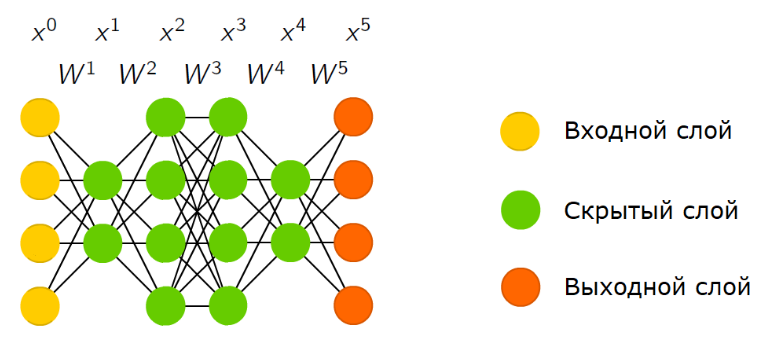
\includegraphics[width=0.6\linewidth]{chapters/neural/images/full_net.png}
	\caption{Полносвязная нейронная сеть.}
	\label{img:full_net}
\end{figure}

Задачей обучения нейронной сети является минимизация средних потерь на обучающей выборке $X$ ($|X| = M$):
$$
Q(\overrightarrow{W}, X) = \frac{1}{m} \sum\limits_{m = 1}^{M} \mathcal{L} (\overrightarrow{W}, x_m) \rightarrow \min_{\overrightarrow{W}}
$$

Пусть объект $x$ описывается вектором признаков $\overrightarrow{x} = [x_1, x_2, \dots, x_n]^T$. В задаче классификации множество ответов $Y$ состоит из $H_L$ элементов. Тогда последний слой нейронной сети $x^{L}$ должен содержать $H_L$ элементов. Нейронная сеть предсказывает ответ $k$, если на её выходе наблюдается вектор $x^L = [0, \dots 0, 1, 0, \dots 0]^T$, где единица стоит на $k$-ом месте. 

Функция потерь может быть, например, квадратичной. Для объекта $x$ функция потерь вычисляется по формуле $\mathcal{L} (\overrightarrow{W}^{(t)}, x) = \frac{1}{2} \sum\limits_{i = 1}^{H_L} (x^L_i ((\overrightarrow{W}^{(t)}, x) - y_i)^2$, где $\overrightarrow{y}$ -- вектор из всех нулей кроме единицы на месте порядкового правильного ответа из множества ответов.

Рассмотрим различные методы обучения полносвязной нейронной сети.

\subsection{Градиентный спуск}

\begin{enumerate}
	\item Выбираем какое-то начальное приближение вектора матриц перехода $\overrightarrow{W}^{(0)}$.
	
	\item Итерационный процесс:
		$$
		\overrightarrow{W}^{(t+1)} = \overrightarrow{W}^{(t)} - h \cdot \overrightarrow{\nabla} Q(\overrightarrow{W}^{(t)}, X)
		$$
		где $h$ -- градиентный шаг или темп обучения.
		
		Для рассмотренного ранее эмпирического риска:
		$$
		\overrightarrow{W}^{(t+1)} = \overrightarrow{W}^{(t)} - \frac{h}{m} \cdot \overrightarrow{\nabla} \sum\limits_{m = 1}^{M} \mathcal{L} (\overrightarrow{W}^{(t)}, x_m)
		$$
		
	\item Повторяем итерационный процесс, пока эмпирический риск $Q(\overrightarrow{W}^{(t)}, X)$ или вектор матриц перехода $\overrightarrow{W}$ не сойдутся. Критерий сходимости может быть абсолютным, то есть когда модуль разности значений на последовательных шагах итерационного процесса меньше какого-то значения $\varepsilon$. Например, для эмпирического риска:
	$$
	\left| Q^{(t + 1)} - Q^{(t)} \right| < \varepsilon
	$$
	Или может быть относительным, когда модуль отношения разности значений на последовательных шагах итерационного процесса к наименьшему, или наибольшему значению, или к первому меньше $\varepsilon$. Например, для эмпирического риска:
	$$
	\left| \frac{Q^{(t + 1)} - Q^{(t)}}{\min \{ Q^{(t + 1)}, Q^{(t)} \} } \right| < \varepsilon
	$$
	При этом для эмпирического риска и для вектора матриц перехода значение $\varepsilon$ может быть разным.
	
	Для вектора матриц перехода можно предложить следующий способ:
	$$
	\left|\left| \overrightarrow{W}^{(t+1)} - \overrightarrow{W}^{(t)} \right|\right|_1 = \sum\limits_{l = 1}^{L} \sum\limits_{m = 1}^{m_l} \sum\limits_{n = 1}^{n_l} |W^l_{mn}{}^{(t+1)} - W^l_{mn}{}^{(t)}|
	$$
	где вектор матрица перехода рассматривается как вектор всех её элементов, и применяется первая норма. Размерность матрицы $W^l$ равна $m_l \times n_l$. $W^l_{mn}{}^{(t)}$ -- это элемент в $m$-ой строке $n$-ого столбца матрицы перехода между слоями $l-1$ и $l$ на шаге $t$ итерационного процесса.
\end{enumerate}

Недостатком данного метода является низкая скорость сходимости. Для ускорения применяется метод стохастического градиентного спуска.

\subsection{Стохастический градиентный спуск}

В отличие от обычного градиентного спуска, в котором вектор матриц перехода изменяется пропорционально градиенту эмпирического риска для всех объектов, в стохастическом градиенте вектор матриц перехода изменяется пропорционально функции потерь для одного объекта.

Алгоритм стохастического градиента:

\begin{enumerate}
	\item Выбираем какое-то начальное приближение вектора матриц перехода $\overrightarrow{W}^{(0)}$. Вычисляем первое приближение эмпирического риска:
	$$
	Q^{(0)}(\overrightarrow{W}^{(0)}, X) = \frac{1}{m} \sum\limits_{m = 1}^{M} \mathcal{L} (\overrightarrow{W}^{(0)}, x_m)
	$$
	
	\item Итерационный процесс: \\
 	Выбираем какой-нибудь объект $x \in X$, например случайным образом или перебираем все элементы $X$ по порядку. Корректируем вектор матриц перехода:
	$$
	\overrightarrow{W}^{(t+1)} = \overrightarrow{W}^{(t)} - h \cdot \overrightarrow{\nabla} \mathcal{L} (\overrightarrow{W}^{(t)}, x)
	$$
	где $h$ -- темп обучения.
	
	Эмпирический риск оценивается по формуле:
	$$
	Q^{(t+1)}(\overrightarrow{W}^{(t+1)}, X) = \lambda \mathcal{L} (\overrightarrow{W}^{(t)}, x) + (1-\lambda)  Q^{(t)}(\overrightarrow{W}^{(t)}, X)
	$$
	где $\lambda$ -- темп забывания предыстории.
	
	Рассмотрим, откуда взялась эта оценка $Q^{(t+1)}$.
	
	Если $Q^{(t)}$ -- среднее арифметическое объектов $\varepsilon_i$, $i = 1, 2, \dots t$, то
	$$
	Q^{(t)} = \frac{1}{t} \varepsilon_t + \frac{1}{t} \varepsilon_{t-1} + \frac{1}{t} \varepsilon_{t-2} + \dots + \frac{1}{t} \varepsilon_{1}
	$$
	$$
	Q^{(t - 1)} = \frac{1}{t-1} \varepsilon_{t-1} + \frac{1}{t-1} \varepsilon_{t-2} + \dots + \frac{1}{t-1} \varepsilon_{1}
	$$
	$Q^{(t)}$ можно выразить через $Q^{(t-1)}$:
	$$
	Q^{(t)} = \frac{1}{t} \varepsilon_t + \frac{t-1}{t} Q^{(t-1)} = \frac{1}{t} \varepsilon_t + (1 - \frac{1}{t}) Q^{(t-1)}
	$$
	
	Если $Q^{(t)}$ -- экспоненциальное скользящее среднее с параметром $\lambda$, то
	$$
	Q^{(t)} = \lambda \varepsilon_t + \lambda (1-\lambda) \varepsilon_{t-1} + \lambda (1-\lambda)^2 \varepsilon_{t-2} + \dots + \lambda (1-\lambda)^{t-1} \varepsilon_{1}
	$$
	$$
	Q^{(t - 1)} = \lambda \varepsilon_{t-1} + \lambda (1-\lambda) \varepsilon_{t-2} + \lambda (1-\lambda)^2 \varepsilon_{t-3} + \dots + \lambda (1-\lambda)^{t-2} \varepsilon_{1}
	$$
	Или $Q^{(t)}$ через $Q^{(t-1)}$:
	$$
	Q^{(t)} = \lambda \varepsilon_t + (1 - \lambda) Q^{(t - 1)}
	$$
	
	Пусть теперь $\lambda \sim \frac{1}{t}$. Тогда $(1-\lambda)^{t-1} = (1 - \frac{1}{t})^{t-1}$. $\lim\limits_{t\rightarrow \infty} (1 - \frac{1}{t})^{t-1} = \frac{1}{e}$. По аналогии из радиотехники, где для экспоненциально убывающего сигнала характерное время затухания измеряется по уменьшению сигнала в $e$ раз, тогда характерное количество членов, когда происходит затухание / <<забывание>> предыдущей истории ряда равно $t$.
		
	\item Повторяем итерационный процесс, пока эмпирический риск $Q(\overrightarrow{W}^{(t)}, X)$ или вектор матриц перехода $\overrightarrow{W}$ не сойдутся.
\end{enumerate}

\subsection{Метод обратного распространения ошибок (BackProp).}

Для вычисления градиента функции потерь применяется метод обратного распространения ошибок. Для упрощения формулы индекс ${}^{(t)}$ будем опускать.
$$
\overrightarrow{\nabla} \mathcal{L} (\overrightarrow{W}, x) = \left[\frac{\partial}{\partial W^0}, \frac{\partial}{\partial W^\partial}, \dots, \frac{\partial}{\partial W^L}\right]^T \cdot \mathcal{L} (\overrightarrow{W}, x)
$$

Для рассмотренной ранее квадратичной функции потерь:
$$
\overrightarrow{\nabla} \mathcal{L} (\overrightarrow{W}, x) = \left[\frac{\partial}{\partial W^0}, \frac{\partial}{\partial W^\partial}, \dots, \frac{\partial}{\partial W^L}\right]^T \cdot \frac{1}{2} \sum\limits_{i = 1}^{H_L} (x^L_i ((\overrightarrow{W}, x) - y_i)
$$
То есть выход нейронной сети $\overrightarrow{x^L}$ является функцией от вектора матриц перехода $\overrightarrow{W}$.

Выведем формулу, по которой нейронная сеть вычисляет $\overrightarrow{x^L}$. На первом слое сети находится вектор $\overrightarrow{x^0}$, который через матрицу перехода $W^1$ и вектор функций активации $\overrightarrow{\sigma_1}$ преобразуется во вход второго слоя $x^1$:
$$
\overrightarrow{x^1} = \overrightarrow{\sigma_1} (W^1 \cdot \overrightarrow{x^0})
$$
Аналогично для последующих слоёв:
$$
\overrightarrow{x^2} = \overrightarrow{\sigma_2} (W^2 \cdot \overrightarrow{x^1}) = \overrightarrow{\sigma_2} (W^2 \cdot \overrightarrow{\sigma_1} (W^1 \cdot \overrightarrow{x^0}))
$$
$$
\overrightarrow{x^L} = \overrightarrow{\sigma_L}(W^L \cdot \overrightarrow{x^{L-1}}) = \overrightarrow{\sigma_L}(W^L \cdot \overrightarrow{\sigma_{L-1}} (W^{L-1} \cdot \overrightarrow{\sigma_{L-1}}( \dots ( W^2 \cdot \overrightarrow{\sigma_1} (W^1 \cdot \overrightarrow{x^0})) \dots ))
$$

Чтобы получить формулы для обратного распространения ошибок необходимо найти $\overrightarrow{\nabla} \mathcal{L}$, рассматривая $\overrightarrow{x^L}$ как функцию $\overrightarrow{x^L} (\overrightarrow{W})$.

\textbf{Задача 3.} Доказать рекуррентные формулы для метода обратного распространения ошибок в предположениях:
\begin{enumerate}
	\item Функция потерь квадратичная $\mathcal{L} (\overrightarrow{W}, x) = \frac{1}{2} \sum\limits_{i = 1}^{H_L} (x^L_i ((\overrightarrow{W}, x) - y_i)^2$.
	
	\item Первый нейрон в слое нейронной сети всегда -1, то есть $\forall i: x^i_0 = -1$. $H_l$ -- количество нейронов в слое $l$ без учёта нейрона -1. Тогда индекс первого нейрона в слое, не всегда равного -1, равен 1, а индекс последнего нейрона равен $H_l$.
	
	\item Вектор функций активации $\overrightarrow{\sigma^l}$ зависит от отступа $\overrightarrow{M^l}$: $\sigma^l_n = \sigma^l_n(M^l_n)$, где $M_n = \sum\limits_{m = 1}^{H_l} W^l_{nm} x^{l-1}_{m}$. $\overrightarrow{M^l} = W^l \overrightarrow{x^{l-1}}$.
\end{enumerate}
$
\frac{\partial \mathcal{L}}{\partial x^L_n} = x^L_n - y_n
$, \\
$
\frac{\partial \mathcal{L}}{\partial W^L_{nm}} = \frac{\partial \mathcal{L}}{\partial x^L_n} \frac{\partial \sigma^L_n}{\partial M^L_n} x^{L-1}_{m}
$, \\
$
\frac{\partial \mathcal{L}}{\partial x^{l}_n} = \sum\limits_{m = 1}^{H_l} \frac{\partial \mathcal{L}}{\partial x^{l+1}_m} \frac{\partial \sigma^{l+1}_m}{\partial M^{l+1}_m} W^{l+1}_{mn}
$, \\
$
\frac{\partial \mathcal{L}}{\partial W^{l}_{nm}} = \frac{\partial \mathcal{L}}{\partial x^{l}_n} \frac{\partial \sigma^{l}_n}{\partial M^{l}_n} x^{l-1}_{m}
$, \\
$1 \le l < L$.

\textbf{Решение:}

Сначала докажем соотношения для $l = L$.

Рассматриваем функцию потерь как сложную функцию $\mathcal{L} (\overrightarrow{W}) = \mathcal{L}(\overrightarrow{x^L}(\overrightarrow{W}))$:
$$
\frac{\partial \mathcal{L}}{\partial {W^{L}_{nm}}} = \sum\limits_{i = 1}^{H_L} \frac{\partial \mathcal{L}}{\partial x^L_i} \frac{\partial x^L_i}{\partial W^L_{nm}}
$$
Матрица $W^{L}$ используется в уравнении: $\overrightarrow{x^L} = \overrightarrow{\sigma^L} (W^L \overrightarrow{x^{L-1}})$. В данном уравнении предполагается, что вектор $\overrightarrow{x^L}$ имеет размерность $H_L \times 1$ (является столбцом, а не строкой) и не содержит -1, так как вес константы $x^L_0$ не вычисляется по предыдущему слою, а определяется нулевым столбцом матрицы $W^{L+1}$, а вектор $\overrightarrow{x^{L-1}}$ уже имеет длину $1+H_{L-1}$, и содержит -1. Тогда размерность матрицы $W^{L}$ равна $H_L \times (1+H_{L-1})$. Дифференцировать $\mathcal{L}$ по $x^L_0$ не имеет смысла, так как всегда $x^L_0 = -1$.

Так как $\mathcal{L} (\overrightarrow{x^L}) = \frac{1}{2} \sum\limits_{n = 1}^{H_L} (x^L_n - y_n)^2$, то
$$
\frac{\partial \mathcal{L}}{\partial x^L_i} = x^L_i - y_i
$$

Так как $\overrightarrow{x^L} = \overrightarrow{\sigma^L}(W^L \overrightarrow{x^{L-1}})$ или $x^L_i = \sigma^L_i\left(\sum\limits_{k = 0}^{H_{L-1}} W^{L}_{ik} x^{L-1}_k\right)$, тогда \\
$\frac{\partial x^L_i}{\partial W^L_{nm}} = 0$, если $n \neq i$ и \\
$\frac{\partial x^L_i}{\partial W^L_{nm}} = \frac{\partial \sigma^L_n}{\partial M^L_n} x^{L-1}_m$, если $n = i$. \\
То есть функция $\sigma^L_i$ зависит от $W^l_{nm}$, если $n = i$. При дифференцировании суммы $\sum\limits_{k = 0}^{H_{L-1}} W^{L}_{ik} x^{L-1}_k$ остаётся только член с $k = m$, то есть $x^{L-1}_m$. Стоит отметить, что функция активации как функция от одного аргумента $\sigma^L_n = \sigma^L_n(M^L_n)$ известна при написании программы, аналогично будет известна и её производная $\frac{\partial \sigma^L_n}{\partial M^L_n}\Big|_{M^L_n}$. Производная вычисляется в точке $M^L_n = \sum\limits_{k = 0}^{H_{L-1}} W^{L}_{nk} x^{L-1}_k$. 

При использовании стохастического градиентного спуска отступ $\overrightarrow{M^l}$ будет вычислен при прямом ходе, при вычислении $\overrightarrow{x^l}$ от объекта $x \in X$. Поэтому для ускорения вычислений можно при прямом ходе вычислять и запоминать значения производных $\frac{\partial \sigma^l_n}{\partial M^l_n}\Big|_{M^l_n}$ в точке $M^l_n$, также на каждом слое нужно запоминать значения $\overrightarrow{x^l}$.

Теперь используя полученные соотношения запишем:
$$
\frac{\partial \mathcal{L}}{\partial {W^{L}_{nm}}} = \sum\limits_{i = 1}^{H_L} \frac{\partial \mathcal{L}}{\partial x^L_i} \frac{\partial x^L_i}{\partial W^L_{nm}} = \frac{\partial \mathcal{L}}{\partial x^L_n} \frac{\partial x^L_n}{\partial W^L_{nm}} = \frac{\partial \mathcal{L}}{\partial x^L_n} \frac{\partial \sigma^L_n}{\partial M^L_n} x^{L-1}_m
$$
где $\frac{\partial \mathcal{L}}{\partial x^L_n} = x^L_n - y_n$.

Теперь докажем формулы для $1 \le l < L$.

$x^l_n = \sigma^l_n\left(\sum\limits_{k = 0}^{H_{l-1}} W^{l}_{nk} x^{l-1}_k\right)$ или $x^l_n = x^l_n (\overrightarrow{W^l}, \overrightarrow{x^{l-1}})$. Тогда
$$
\frac{\partial \mathcal{L}}{\partial W^l_{nm}} = \sum_{i = 1}^{H_l} \frac{\partial \mathcal{L}}{\partial x^l_i} \frac{\partial x^l_i}{\partial W^{l}_{nm}}
$$

Найдём $\frac{\partial \mathcal{L}}{\partial x^l_i}$.
$$
\frac{\partial \mathcal{L}}{\partial x^l_i} = \sum\limits_{j = 1}^{H_{l+1}} \frac{\partial \mathcal{L}}{\partial x^{l+1}_j} \frac{\partial x^{l+1}_j}{\partial x^{l}_i}
$$
Производная $\frac{\partial \mathcal{L}}{\partial x^{l+1}_j}$ уже была вычислена на шаге для $l+1$. Вычислим $\frac{\partial x^{l+1}_j}{\partial x^{l}_i}$. Так как $x^{l+1}_j = \sigma^{l+1}_j\left(\sum\limits_{k = 0}^{H_{l}} W^{l+1}_{jk} x^{l}_k\right)$, то
$$
\frac{\partial x^{l+1}_j}{\partial x^{l}_i} = \frac{\partial \sigma^{l+1}_{j}}{\partial M^{l+1}_j} W^{l+1}_{ji}
$$
Итого
$$
\frac{\partial \mathcal{L}}{\partial x^l_i} = \sum\limits_{j = 1}^{H_{l+1}} \frac{\partial \mathcal{L}}{\partial x^{l+1}_j} \frac{\partial \sigma^{l+1}_{j}}{\partial M^{l+1}_j} W^{l+1}_{ji}
$$

Производная $\frac{\partial x^l_i}{\partial W^{l}_{nm}}$ вычисляется аналогично, как и для $l = L$: \\
$\frac{\partial x^l_i}{\partial W^l_{nm}} = 0$, если $n \neq i$ и \\
$\frac{\partial x^l_i}{\partial W^l_{nm}} = \frac{\partial \sigma^l_n}{\partial M^l_n} x^{l-1}_m$, если $n = i$.

Окончательно
$$
\frac{\partial \mathcal{L}}{\partial W^l_{nm}} = \frac{\partial \mathcal{L}}{\partial x^l_n} \frac{\partial \sigma^l_n}{\partial M^l_n} x^{l-1}_m
$$

\subsection{Алгоритм применения метода обратного распространения ошибки в стохастическом градиентном спуске.}

Рассмотрим подробнее алгоритм применения метода обратного распространения ошибки в стохастическом градиентном спуске.

\begin{enumerate}
	\item Выбираем какое-то начальное приближение вектора матриц перехода $\overrightarrow{W}^{(0)}$. Вычисляем первое приближение эмпирического риска:
	$$
	Q^{(0)}(\overrightarrow{W}^{(0)}, X) = \frac{1}{m} \sum\limits_{m = 1}^{M} \mathcal{L} (\overrightarrow{W}^{(0)}, x_m)
	$$
	
	\item Итерационный процесс: \\
	Выбираем какой-нибудь объект $x \in X$, например случайным образо или перебираем все элементы $X$ по порядку.
	
	Прямой ход. Вычисляем отступ $\overrightarrow{M^l} = W^l \cdot \overrightarrow{x^{l-1}}$.
	Вычисляем и запоминаем значения выходов нейронов $\overrightarrow{x^l} = \overrightarrow{\sigma^l}(\overrightarrow{M^l})$ и производные функций активации $\frac{\partial \overrightarrow{\sigma^l}}{\partial \overrightarrow{M^l}}\Big|_{\overrightarrow{M^l}}$.
	
	Вычисляем для последнего слоя производные от функции потерь:
	$$
	\frac{\partial \mathcal{L}}{\partial x^L_n} = x^L_n - y_n
	$$
	и
	$$
	\frac{\partial \mathcal{L}}{\partial W^L_{nm}} = \frac{\partial \mathcal{L}}{\partial x^L_n} \frac{\partial \sigma^L_n}{\partial M^L_n} x^{L-1}_{m}
	$$
	
	Обратный ход для всех слоёв $1 \le l < L$:
	$$
	\frac{\partial \mathcal{L}}{\partial x^{l}_n} = \sum\limits_{m = 1}^{H_l} \frac{\partial \mathcal{L}}{\partial x^{l+1}_m} \frac{\partial \sigma^{l+1}_m}{\partial M^{l+1}_m} W^{l+1}_{mn}
	$$
	и
	$$
	\frac{\partial \mathcal{L}}{\partial W^{l}_{nm}} = \frac{\partial \mathcal{L}}{\partial x^{l}_n} \frac{\partial \sigma^{l}_n}{\partial M^{l}_n} x^{l-1}_{m}
	$$
	
	В итоге был вычислен градиент функции потерь: $\overrightarrow{\nabla} \mathcal{L} (\overrightarrow{W}^{(t)}, x)$.
	
	Корректируем вектор матриц перехода:
	$$
	\overrightarrow{W}^{(t+1)} = \overrightarrow{W}^{(t)} - h \cdot \overrightarrow{\nabla} \mathcal{L} (\overrightarrow{W}^{(t)}, x)
	$$
	где $h$ -- темп обучения.
	
	Эмпирический риск оценивается по формуле:
	$$
	Q^{(t+1)}(\overrightarrow{W}^{(t+1)}, X) = \lambda \mathcal{L} (\overrightarrow{W}^{(t)}, x) + (1-\lambda)  Q^{(t)}(\overrightarrow{W}^{(t)}, X)
	$$
	где $\lambda$ -- темп забывания предыстории.
	
	\item Повторяем итерационный процесс, пока эмпирический риск $Q(\overrightarrow{W}^{(t)}, X)$ или вектор матриц перехода $\overrightarrow{W}$ не сойдутся.
\end{enumerate}
        
    \clearpage
    \chapter{Метрические методы классификации и регрессии}
    \section*{Часто используемые ядра \(K(r)\)}

\begin{figure}[h]
    \centering
    \includegraphics[width=\textwidth]{chapters/metric/images/I1.png}
    \caption{Графики ядер}
    \label{fig:kernels}
\end{figure}

\begin{align*}
\Pi(r) &= [{\lvert r \rvert \leq 1}] \quad \text{— прямоугольное} \\
T(r) &= (1 - \lvert r \rvert) [{\lvert r \rvert \leq 1}] \quad \text{— треугольное} \\
E(r) &= (1 - r^2) [{\lvert r \rvert \leq 1}] \quad \text{— квадратичное (Епанечникова)} \\
Q(r) &= (1 - r^2)^2 [{\lvert r \rvert \leq 1}] \quad \text{— квартическое} \\
G(r) &= \exp(-2r^2) \quad \text{— гауссовское}
\end{align*}


\section*{Выбор ядра \(K\) и ширины окна \(h\)}

\noindent
\(h \in \{\textcolor{red}{0.1}, 1.0, \textcolor{blue}{3.0}\}\), гауссовское ядро \(K(r) = \exp(-2r^2)\).
Графики с различной шириной окна \(h\):
\begin{align*}
    \centering
    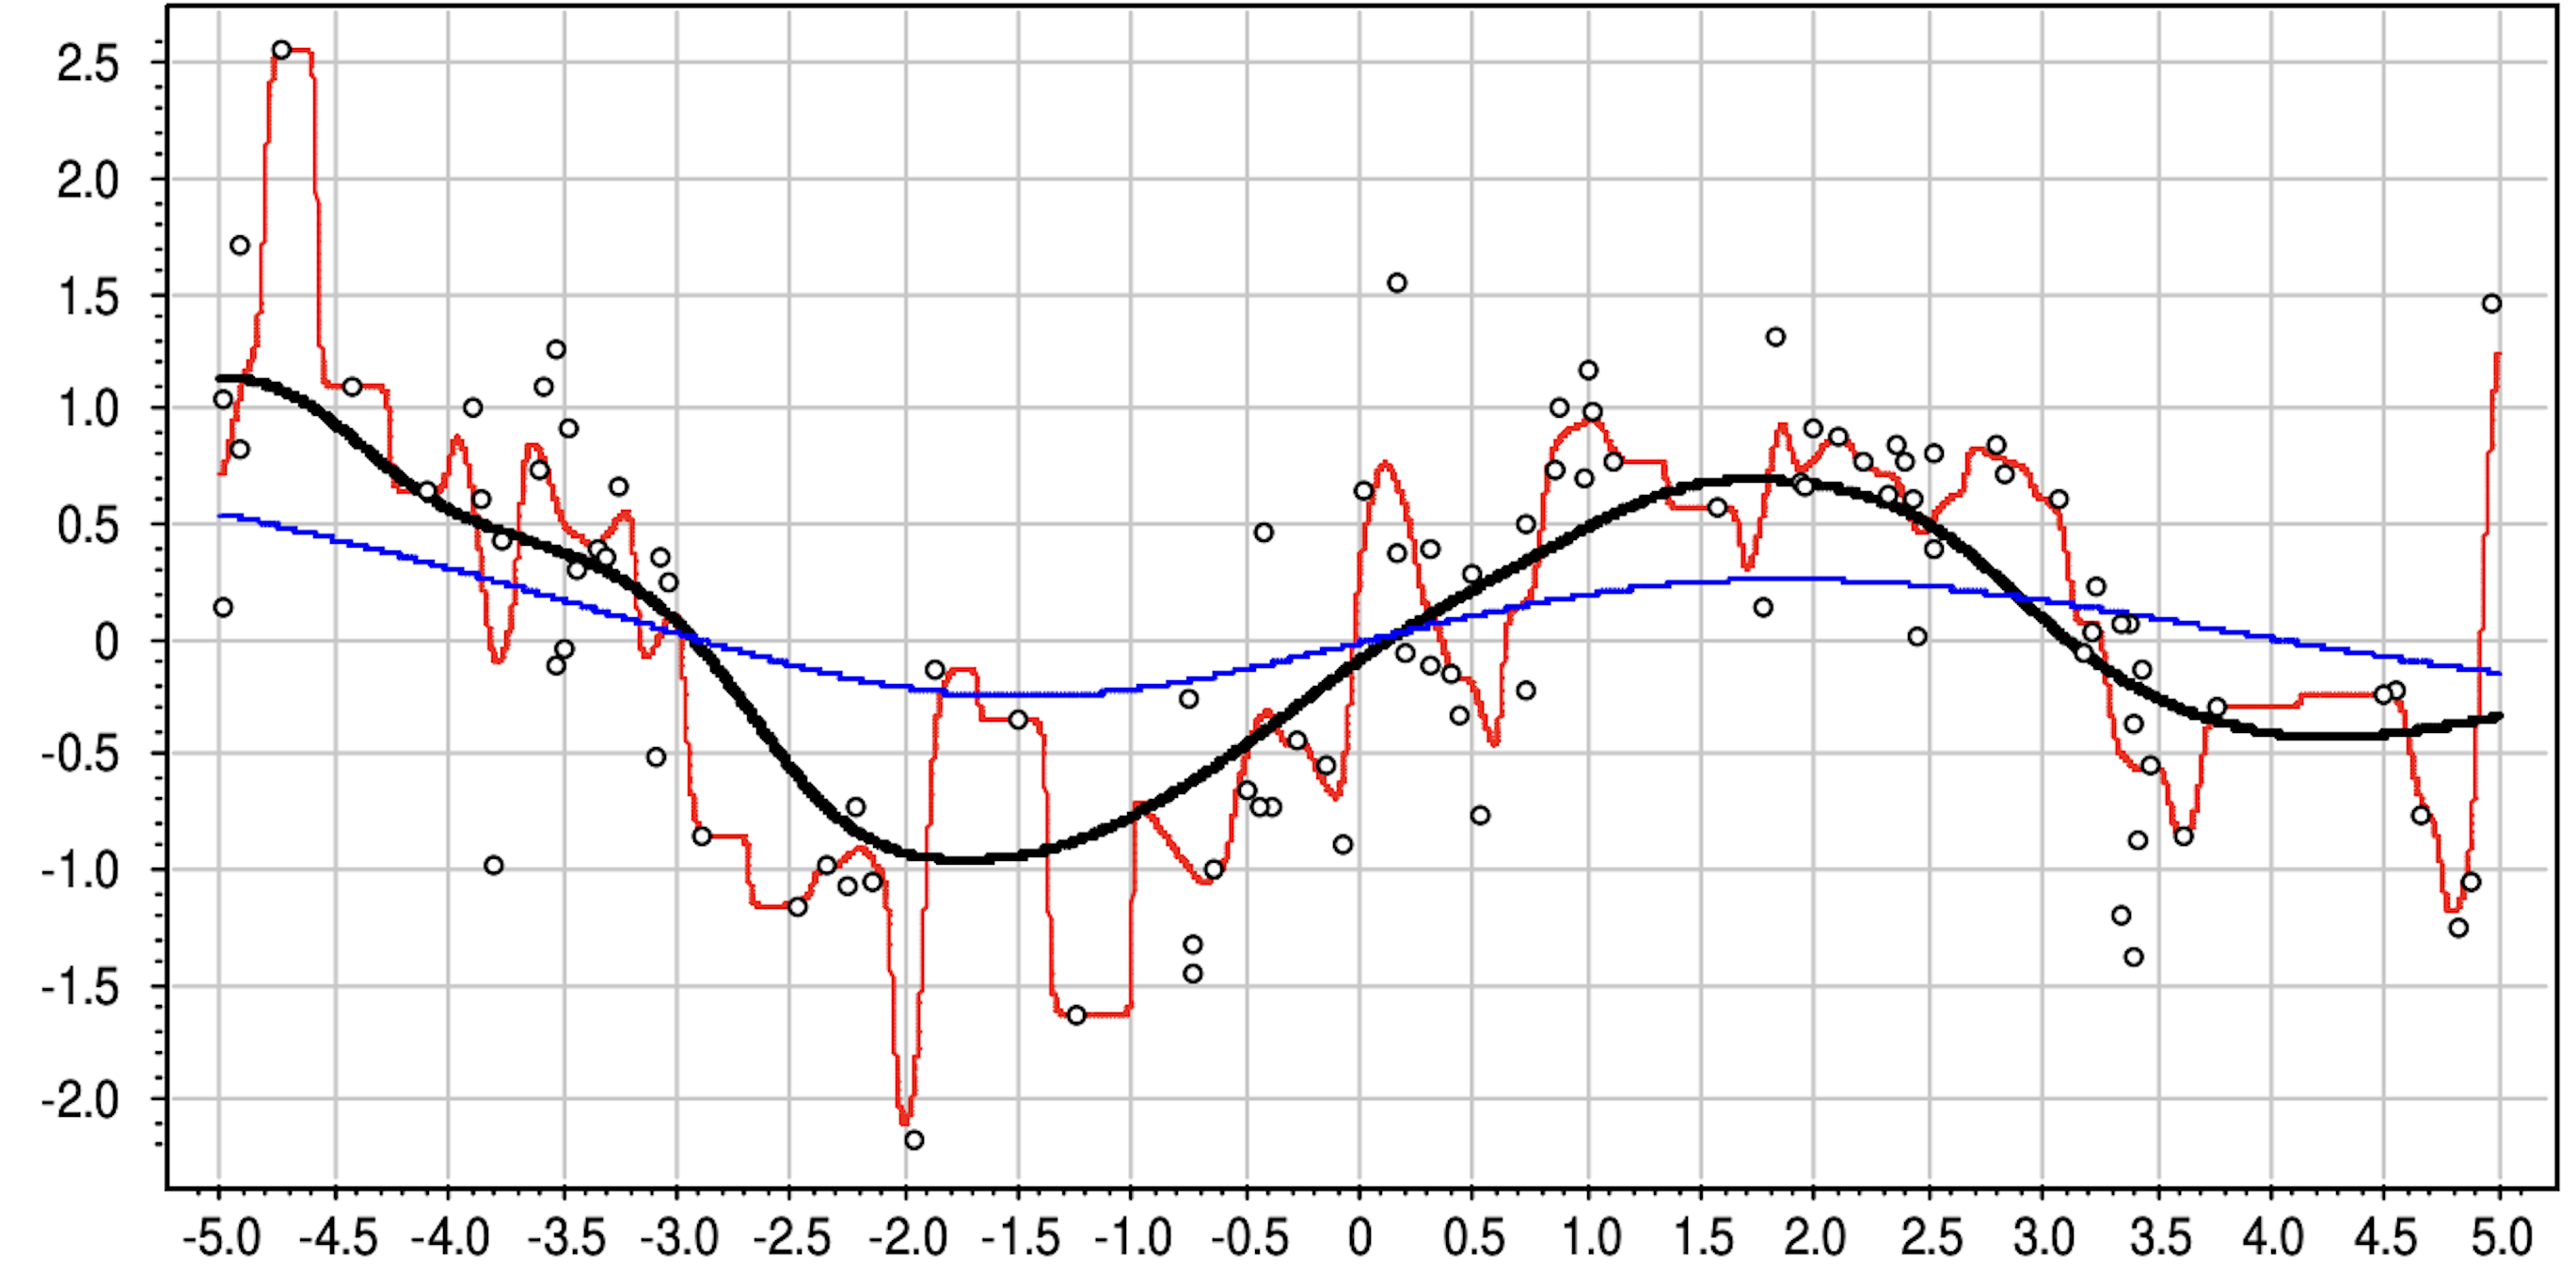
\includegraphics[width=\textwidth]{chapters/metric/images/I2.png}
    \label{fig:kernel_choice}
\end{align*}

\begin{itemize}
    \item Гауссовское ядро \(\Rightarrow\) гладкая аппроксимация
    \item Ширина окна существенно влияет на точность аппроксимации
\end{itemize}

\section*{Выбор ядра \(K\) и ширины окна \(h\)}

\noindent
\(h \in \{\textcolor{red}{0.1}, 1.0, \textcolor{blue}{3.0}\}\), треугольное ядро \(K(r) = (1 - \lvert r \rvert) [{\lvert r \rvert \leq 1}]\). Графики с разными значениями \(h\) при треугольном ядре:
\begin{align*}
    \centering
    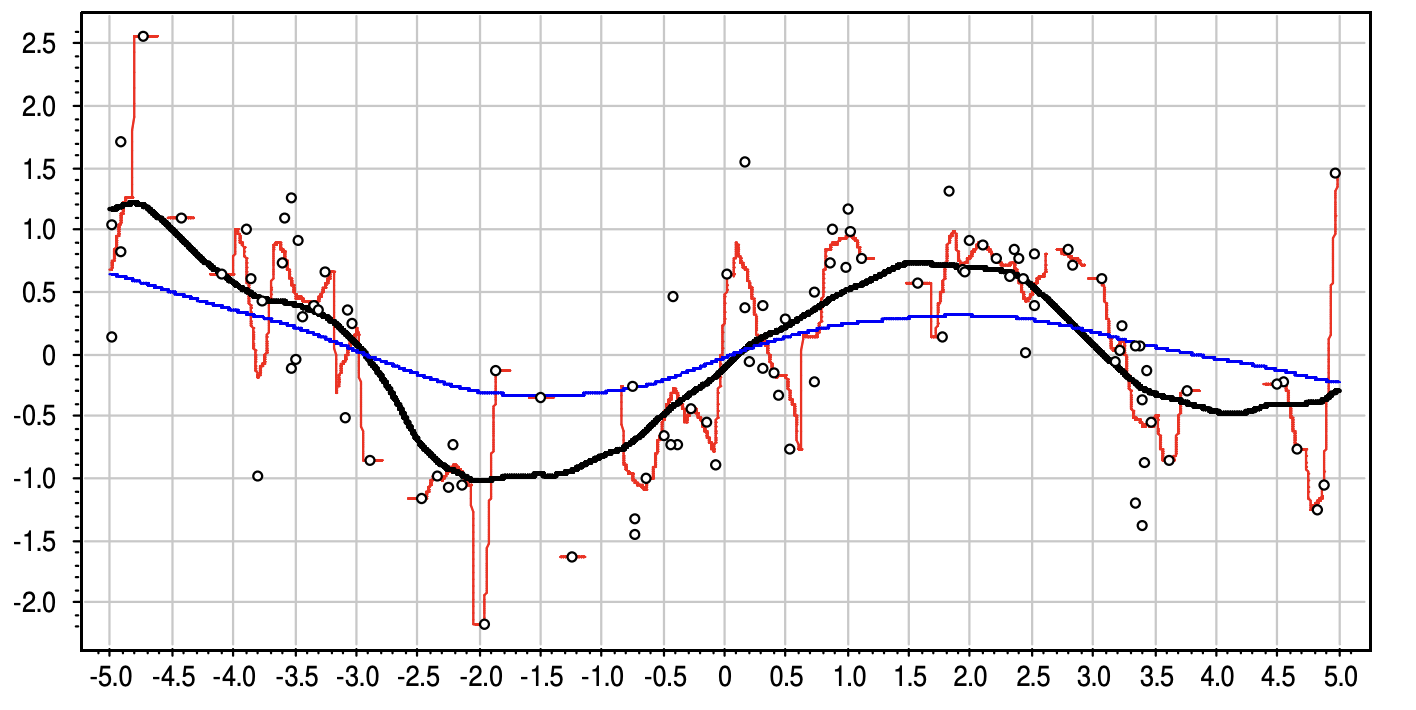
\includegraphics[width=\textwidth]{chapters/metric/images/I3.png}
    \label{fig:kernel_triangle}
\end{align*}

\begin{itemize}
    \item Треугольное ядро \(\Rightarrow\) кусочно-линейная аппроксимация
    \item Аппроксимация не определена, если в окне нет точек выборки
\end{itemize}

\section*{Выбор ядра \(K\) и ширины окна \(h\)}

\begin{itemize}
    \item \textbf{Ядро \(K(r)\)}
    \begin{itemize}
        \item существенно влияет на гладкость функции \( a_h(x) \),
        \item слабо влияет на качество аппроксимации.
    \end{itemize}
    \item \textbf{Ширина окна \(h\)}
    \begin{itemize}
        \item существенно влияет на качество аппроксимации.
    \end{itemize}
    \item \textbf{Переменная ширина окна по \(k\) ближайшим соседям:}
    \[
    w_i(x) = K\left( \frac{\rho(x, x_i)}{h(x)} \right), \quad h(x) = \rho(x, x^{(k+1)})
    \]
    где \(x^{(k)}\) — \(k\)-й сосед объекта \(x\).

    \item \textbf{Оптимизация ширины окна по скользящему контролю:}
    \[
    \text{LOO}(h, X^\ell) = \sum_{i=1}^\ell \left( a_h(x_i; X^\ell \setminus \{x_i\}) - y_i \right)^2 \to \min_h
    \]
\end{itemize}

\section*{Проблема выбросов (эксперимент на синтетических данных)}

\noindent
\(\ell = 100\), \(h = 1.0\), гауссовское ядро \(K(r) = \exp(-2r^2)\)

\vspace{0.5em}

{\color{red}Две из 100 точек — выбросы с ординатами \(y_i = 40\) и \(-40\)}

\vspace{0.5em}

{\color{blue}Синяя кривая — выбросов нет}

\begin{align*}
    \centering
    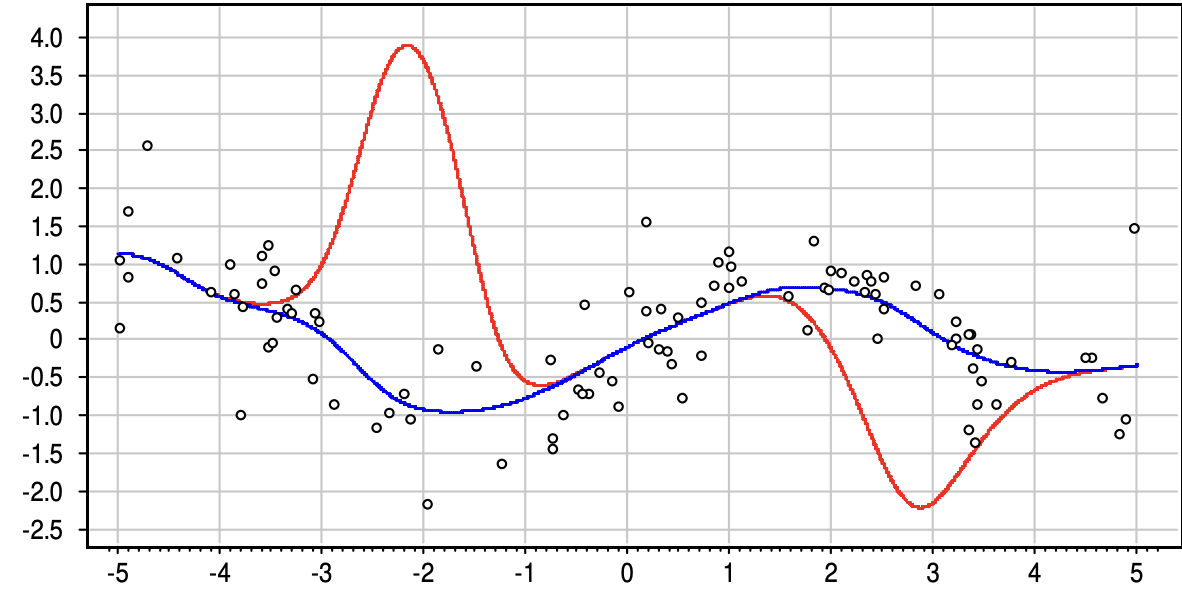
\includegraphics[width=\textwidth]{chapters/metric/images/I4.png}
    \label{fig:kernel_triangle}
\end{align*}

\section*{Проблема выбросов и локально взвешенное сглаживание}

\textbf{Проблема выбросов:} точки с большими случайными ошибками \(y_i\) сильно искажают функцию \(a_h(x)\)

\vspace{1em}
\textbf{Основная идея:} \\
чем больше величина ошибки \(\varepsilon_i = \lvert a_h(x_i; X^\ell \setminus \{x_i\}) - y_i \rvert\), \\
тем больше прецедент \((x_i, y_i)\) похож на выброс, \\
тем меньше должен быть его вес \(w_i(x)\).

\vspace{1em}
\textbf{Эвристика:} \\
домножить веса \(w_i(x)\) на коэффициенты \(\gamma_i = \tilde{K}(\varepsilon_i)\), \\
где \(\tilde{K}\) — ещё одно ядро, вообще говоря, отличное от \(K(r)\).

\vspace{1em}
\textbf{Рекомендация:} \\
квартическое ядро \(\tilde{K}(\varepsilon) = K_Q \left( \frac{\varepsilon}{6 \, \mathrm{med}\{\varepsilon_i\}} \right)\), \\
где \(\mathrm{med}\{\varepsilon_i\}\) — медиана вариационного ряда ошибок.

\section*{Алгоритм LOWESS (LOcally WEighted Scatter plot Smoothing)}

\vspace{1em}
\textcolor{blue}{\textbf{Вход:}} \(X^\ell\) — обучающая выборка; \\
\textcolor{blue}{\textbf{Выход:}} коэффициенты \(\gamma_i, \quad i = 1, \ldots, \ell\);

\vspace{1em}
инициализация: \(\gamma_i := 1, \quad i = 1, \ldots, \ell\);

\vspace{1em}
\textcolor{blue}{\textbf{повторять}}
\begin{itemize}
    \item оценки скользящего контроля в каждом объекте:
    \[
    a_i := a_h(x_i; X^\ell \setminus \{x_i\}) = \frac{\sum\limits_{j=1, j \neq i}^{\ell} y_j \gamma_j K\left( \frac{\rho(x_i, x_j)}{h(x_i)} \right)}{\sum\limits_{j=1, j \neq i}^{\ell} \gamma_j K\left( \frac{\rho(x_i, x_j)}{h(x_i)} \right)}, \quad i = 1, \ldots, \ell;
    \]
    \item \(\gamma_i := \tilde{K}(\lvert a_i - y_i \rvert), \quad i = 1, \ldots, \ell;\)
\end{itemize}

\textcolor{blue}{\textbf{пока}} коэффициенты \(\gamma_i\) не стабилизируются;

\section*{Пример работы LOWESS на синтетических данных}

\noindent
\(\ell = 100\), \(h = 1.0\), гауссовское ядро \(K(r) = \exp(-2r^2)\)

\vspace{1em}

Две из 100 точек — выбросы с ординатами \(y_i = 40\) и \(-40\)

\vspace{1em}

В данном случае LOWESS сходится за несколько итераций:
\begin{align*}
    \centering
    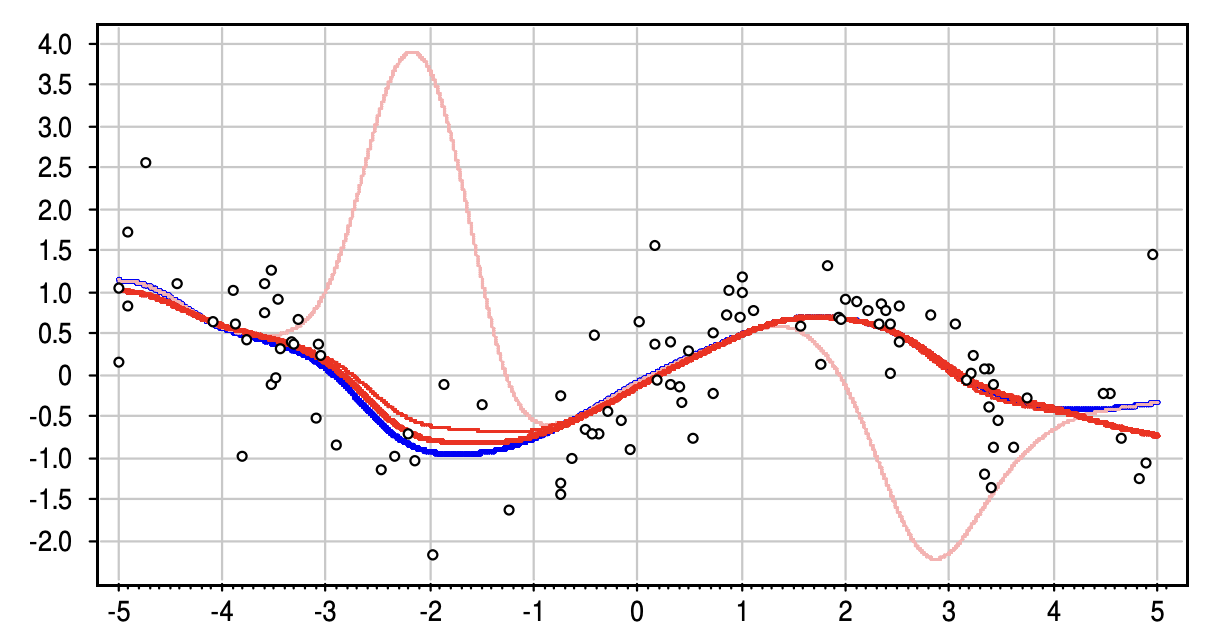
\includegraphics[width=\textwidth]{chapters/metric/images/I5.png}
    \label{fig:kernel_triangle}
\end{align*}

\section{Задачи}
\subsection{Задача 1}
Объясните, как выбор ядра \(K(r)\) влияет на гладкость регрессионной функции \(a_h(x)\). Приведите примеры различных ядер и их влияния.
\subsection{Ответ:}
Ядро \(K(r)\) определяет форму и вес окрестности точки, используемой для оценки регрессионной функции. Гладкие ядра, такие как гауссовское, дают более плавные оценки, в то время как менее гладкие, такие как прямоугольное, приводят к менее сглаженным функциям. Например:

- Гауссовское ядро \(K(r) = \exp(-r^2)\) — даёт плавные, гладкие оценки.

- Треугольное ядро \(K(r) = 1 - \lvert r \rvert\) (при \(\lvert r \rvert \leq 1\)) — более резкое, но все ещё гладкое.

- Прямоугольное ядро \(K(r) = 0.5\) (при \(\lvert r \rvert \leq 1\)) — приводит к кусочно-постоянной функции.

\subsection{Задача 2}
Приведите пример оптимального веса \(w_i(x)\) в алгоритме LOWESS, если известно распределение ошибок в данных. Поясните, как это распределение должно влиять на выбор веса, и почему весовое ядро \(\tilde{K}\) должно учитывать распределение ошибок.

\subsection{Ответ:}
Если ошибка \(\varepsilon_i\) распределена согласно некоторому известному распределению, например нормальному, \( \varepsilon_i \sim \mathcal{N}(0, \sigma^2)\), то весовой коэффициент должен минимизировать дисперсию предсказания. Весовая функция \(\tilde{K}(\varepsilon_i)\) должна убывать, когда \(\varepsilon_i\) отклоняется от некоторого центрального значения (0 для нормального распределения), чтобы уменьшить влияние выбросов:

\[
w_i(x) = \exp\left(-\frac{\varepsilon_i^2}{2\sigma^2}\right)
\]

Этот вес сильнее подавляет ошибки, отклоняющиеся от средней, что уменьшает их влияние на итоговую модель. Выбор весового ядра \(\tilde{K}\) должен учитывать распределение ошибок, чтобы учесть типичные вариации данных.

\subsection{Задача 3}
На основе метода LOWESS предложите способ оценки доверительного интервала для предсказаний. Выведите формулу для доверительного интервала и объясните, как она может быть использована для оценки надежности модели.

\subsection{Ответ:}

\quad 1. Построение модели:

   - Применим LOWESS для построения основной модели, получив предсказанные значения \( \hat{y}_i \) для каждого \(x_i\).

2. Оценка остаточной дисперсии:

   - Вычислим остаточные отклонения \(e_i = y_i - \hat{y}_i\).
   
   - Оценим дисперсию ошибок \(\sigma^2\) как среднеквадратическое отклонение:

     \[
     \sigma^2 = \frac{1}{n-k} \sum_{i=1}^{n} e_i^2
     \]

   где \(n\) — число точек данных, \(k\) — число параметров (в случае LOWESS, это скорее степень полинома в локальных регрессиях).

3. Построение доверительного интервала:

   - Для каждого предсказанного значения \( \hat{y}_i \) построим доверительный интервал, используя стандартное отклонение остаточных ошибок и критические значения из t-распределения:

     \[
     \hat{y}_i \pm t_{\alpha/2, n-k} \cdot \sqrt{\frac{\sigma^2}{n_i}}
     \]

   где \( t_{\alpha/2, n-k} \) — квантиль t-распределения с уровнем значимости \(\alpha\), и \(n_i\) — эффективное число точек в окрестности \(x_i\) (окрестность, которая использовалась для регрессии, может быть выражена размером окна или числом соседей).

4. Использование доверительных интервалов:

   - Доверительные интервалы позволяют пользователю оценить, насколько "надёжны" предсказанные значения. Узкие интервалы свидетельствуют о высокой уверенности.
   
   - Визуализация доверительных интервалов на графиках помогает выявлять области, где модель может быть неопределённой или подверженной ошибкам.

\section{Влияние выбора метрики на качество работы kNN}

Метод \(k\)-ближайших соседей (kNN) является одним из базовых алгоритмов машинного обучения и широко применяется в задачах классификации и регрессии. Этот алгоритм относится к метрическим методам, так как выбор ближайших соседей основывается на измерении расстояний между объектами. Главным фактором, определяющим качество модели, является выбор метрики расстояния, так как она определяет, какие объекты считаются «похожими».

\subsection{Сущность метода \(k\)-ближайших соседей}

Алгоритм \(k\)-ближайших соседей работает следующим образом:
\begin{enumerate}
    \item Для нового объекта вычисляется расстояние до всех объектов обучающей выборки.
    \item Выбираются \(k\) ближайших объектов в соответствии с выбранной метрикой.
    \item Класс нового объекта определяется на основе классов выбранных соседей (например, по принципу большинства для задач классификации).
    \item В задачах регрессии целевое значение нового объекта вычисляется как среднее (или взвешенное среднее) значений соседей.
\end{enumerate}

Ключевым аспектом метода является расстояние, вычисляемое на основе метрики, которая влияет на работу алгоритма, в том числе на точность и устойчивость модели.

\subsection{Популярные метрики расстояния}

\begin{enumerate}
    \item \textbf{Евклидова метрика} (\(L2\)-норма):  
    Одна из самых популярных метрик, измеряющая геометрическое расстояние между точками в пространстве.  
    Формула:
    \[
    d(x, y) = \sqrt{\sum_{i=1}^{n}(x_i - y_i)^2}
    \]
    Особенности:
    \begin{itemize}
        \item Подходит для данных, где все признаки одинаково масштабированы.
        \item Чувствительна к выбросам, так как квадрат отклонения значительно увеличивает вклад большого расхождения.
    \end{itemize}

    \item \textbf{Манхэттенская метрика} (\(L1\)-норма):  
    Измеряет расстояние как сумму абсолютных разностей координат.  
    Формула:
    \[
    d(x, y) = \sum_{i=1}^{n}|x_i - y_i|
    \]
    Особенности:
    \begin{itemize}
        \item Лучше подходит для разреженных данных.
        \item Менее чувствительна к выбросам по сравнению с Евклидовой метрикой.
    \end{itemize}

    \item \textbf{Метрика Минковского}:  
    Обобщение Евклидовой и Манхэттенской метрик.  
    Формула:
    \[
    d(x, y) = \left(\sum_{i=1}^{n}|x_i - y_i|^p\right)^{\frac{1}{p}}
    \]
    Особенности:
    \begin{itemize}
        \item При \(p=2\) совпадает с Евклидовой метрикой, при \(p=1\) — с Манхэттенской.
        \item Позволяет гибко настраивать степень влияния больших отклонений через параметр \(p\).
    \end{itemize}

    \item \textbf{Косинусное расстояние}:  
    Измеряет угол между векторами, игнорируя их длину.  
    Формула:
    \[
    d(x, y) = 1 - \frac{\langle x, y \rangle}{\|x\| \cdot \|y\|}
    \]
    Особенности:
    \begin{itemize}
        \item Часто применяется для текстовых данных (например, векторов TF-IDF).
        \item Устойчиво к изменениям масштаба векторов.
    \end{itemize}

    \item \textbf{Метрика Чебышёва}:  
    Учитывает максимальное различие по одной из координат.  
    Формула:
    \[
    d(x, y) = \max_{i}|x_i - y_i|
    \]
    Особенности:
    \begin{itemize}
        \item Удобна для задач, где критически важно учитывать наибольшее расхождение.
        \item Формирует кубические границы ближайших соседей.
    \end{itemize}
\end{enumerate}

\subsection{Влияние выбора метрики на качество работы модели}

Выбор метрики может значительно изменить поведение алгоритма \(k\)-ближайших соседей. Основные факторы влияния:

\begin{enumerate}
    \item \textbf{Геометрия данных:}  
    Разные метрики формируют разные границы классов. Например, Евклидова метрика создает округлые границы, а Манхэттенская — прямоугольные. В задачах с нелинейными разделяющими гиперплоскостями может потребоваться комбинированный подход или нестандартные метрики.

    \item \textbf{Масштаб признаков:}  
    Метрики, такие как Евклидова, чувствительны к различиям в масштабе признаков. Например, если один признак имеет диапазон [0, 1], а другой — [0, 1000], последний будет доминировать. Для решения этой проблемы применяется нормализация или стандартизация данных.

    \item \textbf{Шум и выбросы:}  
    Метрики по-разному реагируют на шум. Евклидова метрика чувствительна к выбросам, так как квадратичное расстояние значительно увеличивается для больших расхождений. Метрики, такие как Манхэттенская или косинусное расстояние, менее чувствительны к шуму.

    \item \textbf{Высокая размерность:}  
    В задачах с большим количеством признаков (проблема «проклятия размерности») расстояния между всеми объектами становятся примерно одинаковыми. Это снижает различимость ближайших соседей, что делает выбор метрики критически важным.

    \item \textbf{Специфика задачи:}  
    Например, для задач обработки текстов косинусная метрика часто оказывается лучше, так как она учитывает только направление векторов, игнорируя их длину. Для задач с пространственными данными чаще применяются Евклидова или Манхэттенская метрика.
\end{enumerate}

\subsection{Примеры задач}

\begin{enumerate}
    \item \textbf{Теоретическая задача:}  
    Рассмотрите два набора данных из двух классов, представленных точками на плоскости.  
    Постройте границы разделения классов при использовании:
    \begin{itemize}
        \item Евклидовой метрики,
        \item Манхэттенской метрики.
    \end{itemize}
    Объясните, как выбор метрики влияет на форму границ.

    \item \textbf{Практическая задача:}  
    Используя набор данных \texttt{Iris}, обучите модель \(k\)-ближайших соседей с Евклидовой, Манхэттенской и косинусной метриками. Сравните метрики качества (точность, F1-меру) и сделайте вывод о том, какая метрика работает лучше и почему.

    \item \textbf{Исследовательская задача:}  
    Для синтетических данных с перекрывающимися классами разработайте алгоритм выбора оптимальной метрики с использованием кросс-валидации. Постройте графики зависимости точности от параметра \(k\) для разных метрик.
\end{enumerate}

\subsection{Заключение}

Выбор метрики расстояния является ключевым фактором, определяющим качество работы метода \(k\)-ближайших соседей. Оптимальная метрика зависит от природы данных, задачи и требований к точности и устойчивости модели. Для улучшения результатов рекомендуется проводить предварительный анализ данных, нормализацию признаков и тестирование нескольких метрик с использованием кросс-валидации.

    \clearpage
    \chapter{Метод опорных векторов}
    \section{SVM-регрессия}
\subsection{Постановка задачи}
\par В задаче регрессии требуется найти функцию \( f(x) = w^T \phi(x) + b \), которая аппроксимирует целевые значения \( y \) на основе входных данных \( x \), минимизируя ошибки предсказания.
\par В SVM-регрессии вводится допустимая область погрешностей — \(\epsilon\)-окрестность. Это означает, что отклонения \( |f(x_i) - y_i| \) в пределах \(\epsilon\) считаются несущественными, и модель игнорирует их. Цель — минимизировать сложность модели, связанную с \(\|w\|\), штрафуя при этом за отклонения, выходящие за пределы \(\epsilon\).

\subsection{Прямая задача}
\par\textbf{Функция потерь.}  
Для задачи SVM-регрессии используется \(\epsilon\)-чувствительная функция потерь:
\begin{equation*}
    L_\epsilon(f(x), y) = 
    \begin{cases} 
        0, & \text{если } |f(x) - y| \leq \epsilon, \\ 
        |f(x) - y| - \epsilon, & \text{иначе.}
    \end{cases}
\end{equation*}
\noindent\textbf{Прямая постановка задачи:}
\begin{equation*}
    \min_{w, b} \frac{1}{2} \|w\|^2 + C \sum_{i=1}^n L_\epsilon(f(x_i), y_i),
\end{equation*}
где:
\begin{itemize}
    \item \(\|w\|^2\) — регуляризационный член, минимизирующий сложность модели,
    \item \(C\) — коэффициент, регулирующий баланс между штрафами за ошибки и сложностью модели,
    \item \(L_\epsilon(f(x_i), y_i)\) — штраф за выход за пределы \(\epsilon\)-окрестности.
\end{itemize}

\subsection{Преобразование задачи}
\par Для учёта отклонений выше \(\epsilon\) вводятся штрафные переменные \(\xi_i\) и \(\xi_i^*\):  
\begin{itemize}
    \item \(\xi_i\) — превышение сверху (\(y_i > f(x_i) + \epsilon\)),
    \item \(\xi_i^*\) — превышение снизу (\(y_i < f(x_i) - \epsilon\)).
\end{itemize}
\par Задача минимизации принимает вид:
\begin{equation*}
    \min_{w, b, \xi, \xi^*} \frac{1}{2} \|w\|^2 + C \sum_{i=1}^n (\xi_i + \xi_i^*),
\end{equation*}
при ограничениях:
\begin{equation*}
\begin{aligned}
    y_i - (w^T \phi(x_i) + b) \leq \epsilon + \xi_i, \\
    (w^T \phi(x_i) + b) - y_i \leq \epsilon + \xi_i^*, \\
    \xi_i, \xi_i^* \geq 0.
\end{aligned}
\end{equation*}

\subsection{Метод Лагранжа}
\par Для решения задачи вводится лагранжиан, который включает:
\begin{itemize}
    \item Целевую функцию,
    \item Ограничения через множители Лагранжа (\(\alpha, \alpha^*, \eta, \eta^*\)).
\end{itemize}
\par Лагранжиан записывается как:
\begin{equation*}
\begin{aligned}
    L(w, b, \xi, \xi^*, \alpha, \alpha^*, \eta, \eta^*) &= \frac{1}{2} \|w\|^2 + C \sum_{i=1}^n (\xi_i + \xi_i^*) - \\
    &\quad - \sum_{i=1}^n \alpha_i \big[ \epsilon + \xi_i - y_i + w^T \phi(x_i) + b \big] - \\
    &\quad - \sum_{i=1}^n \alpha_i^* \big[ \epsilon + \xi_i^* + y_i - w^T \phi(x_i) - b \big] - \\
    &\quad - \sum_{i=1}^n (\eta_i \xi_i + \eta_i^* \xi_i^*).
\end{aligned}
\end{equation*}
\par Для нахождения двойственной задачи необходимо минимизировать \(L\) по \(w\), \(b\), \(\xi\), \(\xi^*\) и максимизировать по множителям Лагранжа.

\subsection{Условия оптимальности}
\begin{enumerate}
    \item Производная по \(w\):
    \begin{equation*}
        \frac{\partial L}{\partial w} = w - \sum_{i=1}^n (\alpha_i - \alpha_i^*) \phi(x_i) = 0 \implies 
        w = \sum_{i=1}^n (\alpha_i - \alpha_i^*) \phi(x_i).
    \end{equation*}
    \item Производная по \(b\):
    \begin{equation*}
        \frac{\partial L}{\partial b} = \sum_{i=1}^n (\alpha_i - \alpha_i^*) = 0.
    \end{equation*}
    \item Производные по \(\xi_i\) и \(\xi_i^*\):
    \begin{equation*}
        \alpha_i + \eta_i = C, \quad \alpha_i^* + \eta_i^* = C, \quad 0 \leq \alpha_i, \alpha_i^* \leq C.
    \end{equation*}
\end{enumerate}

\subsection{Двойственная задача}
\par Подставляя условия оптимальности в лагранжиан, исключаем \(w\), \(b\), \(\xi_i\), \(\xi_i^*\). Получаем двойственную задачу:
\begin{equation*}
    \max_{\alpha, \alpha^*} -\frac{1}{2} \sum_{i,j=1}^n (\alpha_i - \alpha_i^*)(\alpha_j - \alpha_j^*) K(x_i, x_j) 
    - \epsilon \sum_{i=1}^n (\alpha_i + \alpha_i^*) + \sum_{i=1}^n y_i (\alpha_i - \alpha_i^*),
\end{equation*}
где \(K(x_i, x_j) = \phi(x_i)^T \phi(x_j)\) — ядровая функция.
\par Ограничения:
\begin{equation*}
    \sum_{i=1}^n (\alpha_i - \alpha_i^*) = 0, \quad 0 \leq \alpha_i, \alpha_i^* \leq C.
\end{equation*}
\par Для решения двойственной задачи используется метод квадратичного программирования.

\subsection{Построение финальной модели}
\par После решения двойственной задачи оптимальные \(\alpha_i\) и \(\alpha_i^*\) определяют параметры модели:
\begin{equation*}
    f(x) = \sum_{i=1}^n (\alpha_i - \alpha_i^*) K(x_i, x) + b.
\end{equation*}
\par Смещение \(b\) вычисляется через опорные векторы — точки, где выполняется одно из условий:
\begin{equation*}
    y_i - (w^T \phi(x_i) + b) = \epsilon, \quad \text{или} \quad y_i - (w^T \phi(x_i) + b) = -\epsilon.
\end{equation*}
\par Опорные векторы (\(\alpha_i > 0\) или \(\alpha_i^* > 0\)) определяют форму модели.

\subsection{Выбор ядра}
\par Выбор ядра играет ключевую роль в качестве работы модели SVM-регрессии. Различные ядра по-разному преобразуют входные данные, что может существенно повлиять на точность предсказаний и обобщающую способность модели.
\par Выбор ядра зависит от особенностей данных, структуры зависимости и доступных вычислительных ресурсов. Экспериментальная проверка нескольких типов ядер и последующая оценка метрик качества модели — это ключевой этап в процессе выбора оптимального ядра.
\par На рисунке ниже представлена SVM-регрессия с тремя типами ядер: RBF, линейным и полиномиальным. 
\begin{figure}[h!]
    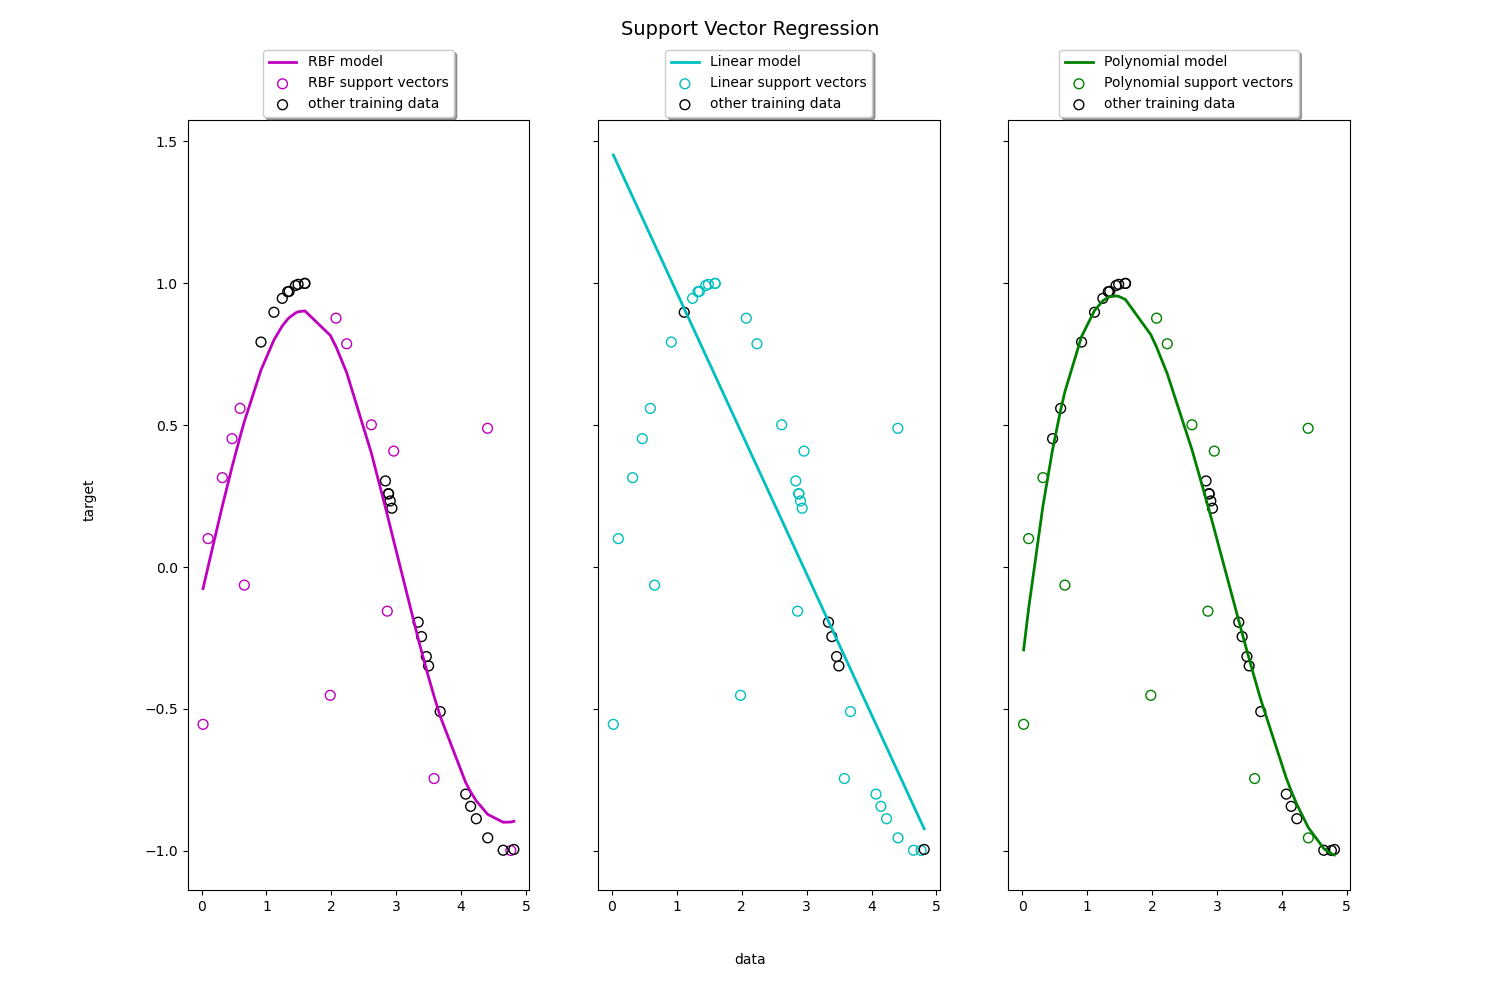
\includegraphics[width = 0.8\textwidth]{MLbook/chapters/svm/images/svm_regression_cmp_models.png}
    \centering
    \caption{Сравнение SVM-регрессия с разными типами ядер}
    \label{fig:kernel_comparison}
\end{figure}

\subsection{Задача 1}
\textbf{Условие}:
\par Рассмотрим следующий набор точек, лежащих на границе \(\epsilon\) - окрестности для SVM-регрессии с линейным ядром:
\begin{equation*}
    \{(1, 2), (2, 3), (3, 5), (4, 6)\}
\end{equation*}
\par Постройте регрессионную модель и найдите смещение \(b\), если \(w = 2\), \(\epsilon = 1\).
\par \noindent \textbf{Решение:}
\par Для нахождения смещения \(b\) необходимо использовать точки, которые лежат на границах \(\epsilon\)-окрестности. Мы знаем, что для таких точек выполняется равенство:
\begin{equation*}
    y_i - (w x_i + b) = \epsilon \quad \text{или} \quad y_i - (w x_i + b) = -\epsilon
\end{equation*}
\par Найдем для каждой точки \(b\), подставив их координаты в эти уравнения:
\begin{itemize}
\item Для точки \((1, 2)\):
\begin{equation*}
    2 - (2 \cdot 1 + b) = 1 \quad \Rightarrow \quad 2 - (2 + b) = 1 \quad \Rightarrow \quad -b = 1 \quad \Rightarrow \quad b = -1
\end{equation*}
\item Для точки \((2, 3)\):
\begin{equation*}
    3 - (2 \cdot 2 + b) = 1 \quad \Rightarrow \quad 3 - (4 + b) = 1 \quad \Rightarrow \quad -b = 2 \quad \Rightarrow \quad b = -2
\end{equation*}
\item Для точки \((3, 5)\):
\begin{equation*}
    5 - (2 \cdot 3 + b) = 1 \quad \Rightarrow \quad 5 - (6 + b) = 1 \quad \Rightarrow \quad -b = 2 \quad \Rightarrow \quad b = -2
\end{equation*}
\item Для точки \((4, 6)\):
\begin{equation*}
    6 - (2 \cdot 4 + b) = 1 \quad \Rightarrow \quad 6 - (8 + b) = 1 \quad \Rightarrow \quad -b = 3 \quad \Rightarrow \quad b = -3
\end{equation*}
\end{itemize}
\par Для вычисления окончательного значения смещения \(b\), усредняем найденные значения:
\begin{equation*}
    b_{\text{avg}} = \frac{-1 + (-2) + (-2) + (-3)}{4} = \frac{-8}{4} = -2
\end{equation*}
\par Таким образом, смещение \(b = -2\).
\par Регрессионная модель для SVM с линейным ядром имеет следующий вид:
\begin{equation*}
    f(x) = w x + b
\end{equation*}
\par Подставляем данное в условии значения \(w = 2\) и найденное значение \(b = -2\):
\begin{equation*}
    f(x) = 2x - 2
\end{equation*}
\par Это и есть наша линейная регрессионная модель.
\par \noindent \textbf{Ответ:} \(f(x) = 2x - 2\).

\subsection{Задача 2}
\textbf{Условие:}
\par У нас есть два набора данных для задачи регрессии:
\begin{itemize}
    \item Набор 1: \( \{(1, 2), (2, 3), (3, 4), (4, 5)\} \)    
    \item Набор 2: \( \{(1, 1), (2, 4), (3, 9), (4, 16)\} \)  
\end{itemize}
\par Предположим, что мы используем SVM-регрессию с различными типами ядер (линейное, полиномиальное, RBF). Определите, какое ядро будет оптимальным для каждого набора данных.
\par \noindent \textbf{Решение:}
\begin{itemize}
    \item Набор 1: данные имеют линейную зависимость, следовательно, линейное ядро будет лучшим выбором.

    \item Набор 2: данные имеют квадратичную зависимость, следовательно, оптимально будет использовать полиномиальное ядро второй степени.
\end{itemize}
\par \noindent \textbf{Ответ:} для первого набора данных оптимальным ядром будет линейное, для второго набора данных - полиномиальное второй степени.

\subsection{Задача 3}
\textbf{Условие:}
\par Дан набор данных для SVM-регрессии с линейным ядром: 
\begin{equation*}
    \{(1, 2), (2, 2.8), (3, 5.2), (4, 8)\}.
\end{equation*}
\par Параметры модели: \(w = 1.5\), \(b = 0.5\), \(\epsilon = 0.5\). 
\begin{enumerate}
    \item Определите, какие из точек набора данных находятся вне \(\epsilon\)-окрестности (требуют штрафных переменных \(\xi\) или \(\xi^*\)).
    \item Вычислите значения штрафных переменных для этих точек.
\end{enumerate}
\par \noindent \textbf{Решение:}
\begin{enumerate}
\item Определение границ \(\epsilon\)-окрестности:
   Уравнение модели SVM-регрессии с линейным ядром: 
   \begin{equation*}
    f(x) = wx + b.
   \end{equation*}
   Подсталяем данные в условии значения:
   \begin{equation*}
    f(x) = 1.5x + 0.5.
   \end{equation*}
   Границы \(\epsilon\)-окрестности:
   \begin{equation*}
    f(x) - \epsilon \leq y \leq f(x) + \epsilon.
   \end{equation*}
\item Проверка точек:
\begin{itemize}
    \item Для точки \((1, 2)\): 
    \begin{equation*}
        f(1) = 1.5 \cdot 1 + 0.5 = 2.0, \quad 2 - 0.5 \leq 2 \leq 2 + 0.5 \quad (\text{в окрестности}).
    \end{equation*}
    \item Для точки \((2, 2.8)\): 
    \begin{equation*}
        f(2) = 1.5 \cdot 2 + 0.5 = 3.5, \quad 3.5 - 0.5 \not\leq 2.8 \leq 3.5 + 0.5 \quad (\text{вне окрестности}).
    \end{equation*}
    \item Для точки \((3, 5.2)\): 
    \begin{equation*}
        f(3) = 1.5 \cdot 3 + 0.5 = 5.0, \quad 5.0 - 0.5 \leq 5.2 \leq 5.0 + 0.5 \quad (\text{в окрестности}).
    \end{equation*}
    \item Для точки \((4, 8)\): 
    \begin{equation*}
        f(4) = 1.5 \cdot 4 + 0.5 = 6.5, \quad 6.5 - 0.5 \leq 8.0 \not\leq 6.5 + 0.5 \quad (\text{вне окрестности}).
    \end{equation*}
\end{itemize}
\item Штрафные переменные:
\begin{itemize}
    \item Для точки \((2, 2.8)\):
    \begin{equation*}
        \xi_i = f(2) - y - \epsilon = 3.5 - 2.8 - 0.5 = 0.2.
    \end{equation*}
    \item Для точки \((4, 8)\):
    \begin{equation*}
        \xi_i^* = y - f(4) - \epsilon = 8 - 6.5 - 0.5 = 1.0.
    \end{equation*}
\end{itemize}
Таким образом, штрафные переменные:
\begin{equation*}
    \xi_2^* = 0.2, \quad \xi_4 = 1.0.
\end{equation*}
\end{enumerate}
\par \noindent \textbf{Ответ:} \(\xi_2^* = 0.2, \quad \xi_4 = 1.0.\)


\setcounter{secnumdepth}{0}

\section{1-norm SVM (LASSO SVM)}
\subsection*{Аппроксимация эмпирического риска с \(L_1\)-регуляризацией}
\begin{align*}
    \sum_{i=1}^{\ell} \left(1 - M_i(w, w_0)\right)_+ + \mu \sum_{j=1}^{n} |w_j| & \rightarrow \min_{w, w_0}
\end{align*}

\subsection*{Плюс: отбор признаков с параметром селективности \(\mu\)}
\begin{itemize}
    \item чем больше \(\mu\), тем меньше признаков останется
\end{itemize}

\subsection*{Минус: слишком агрессивный отбор признаков}
\begin{itemize}
    \item по мере увеличения \(\mu\) признак может быть отброшен, хотя $y$ существенно зависит от него (даже когда ещё не все шумовые признаки отброшены)
\end{itemize}

\newline
\newline

\section{Сравнение \(L_2\) и \(L_1\) регуляризации}

Зависимость весов \(w_j\) от коэффициента \(\frac{1}{\mu}\):

\begin{itemize}
    \item \(L_1\) регуляризатор: \(\mu \sum_{j} |w_j|\)
\end{itemize}

\begin{align*}
    \centering
    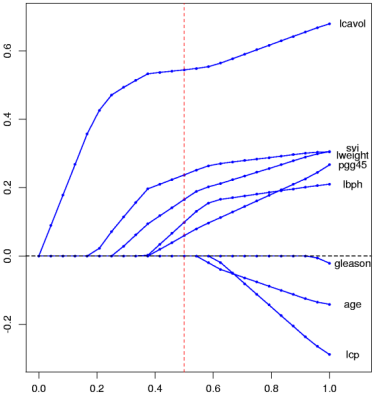
\includegraphics[width=0.6 \linewidth]{chapters/svm/images/L_1.png}
    \label{fig:image}    
\end{align*}

\begin{itemize}
    \item \(L_2\) регуляризатор: \(\mu \sum_{j} w_j^2\)
\end{itemize}

\begin{align*}
    \centering
    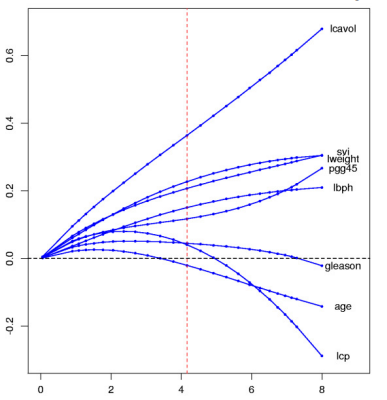
\includegraphics[width=0.6 \linewidth]{chapters/svm/images/L_2.png}
    \label{fig:image}    
\end{align*}

\section{Doubly Regularized SVM (Elastic Net SVM)}

\begin{align*}
    C \sum_{i=1}^{\ell} \left(1 - M_i(w, w_0)\right)_+ + \mu \sum_{j=1}^{n} |w_j| + \frac{1}{2} \sum_{j=1}^{n} w_j^2 & \rightarrow \min_{w, w_0}
\end{align*}

\subsection*{Плюсы:}
\begin{itemize}
    \item Параметр селективности \(\mu\) управляет отбором признаков: чем больше \(\mu\), тем меньше признаков останется
    \item Есть эффект группировки (grouping effect): значимые зависимые признаки отбираются вместе
\end{itemize}

\subsection*{Минусы:}
\begin{itemize}
    \item Шумовые признаки также группируются и могут вместе оставаться в модели
    \item Приходится подбирать два параметра регуляризации \(\mu, \tau\) (есть специальные методы, например, regularization path)
\end{itemize}

\subsection{Elastic Net Analysis}

Elastic Net менее жёстко отбирает признаки.

\begin{figure}[h]
    \centering
    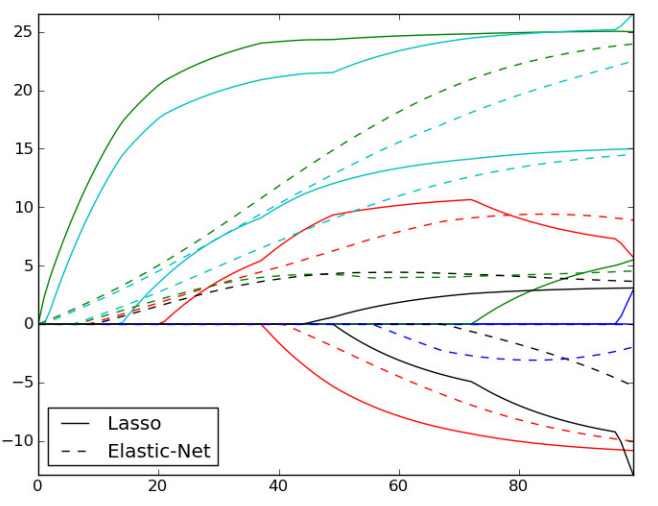
\includegraphics[width=0.8\linewidth]{chapters/svm/images/Elastic_Net.png}
    \caption{Зависимости весов \(w_j\) от коэффициента \(\log \frac{1}{\mu}\)}
    \label{fig:mpr}
\end{figure}

\section{Support Features Machine (SFM)}

\begin{align*}
    C \sum_{i=1}^{\ell} \left(1 - M_i(w, w_0)\right)_+ + \sum_{j=1}^{n} R_{\mu}(w_{j}) & \rightarrow \min_{w, w_0}
\end{align*}

\begin{align*}
R_{\mu}(w_j)=
    \begin{cases}
        2\mu |w_j|, & |w_j| \leq \mu\\
        \mu^2 + w_j^2, & |w_j| \geq \mu \\
    \end{cases}
\end{align*}

\subsection*{Плюсы}
\begin{itemize}
    \item Только один параметр регуляризации \(\mu\)
    \item Отбор признаков с параметром селективности \(\mu\)
    \item Эффект группировки: значимые зависимые признаки ($|w_j|$ > \(\mu\)) входят в решение совместно (как в $Elastic$ $Net$)
    \item Шумовые признаки ($|w_j|$ < \(\mu\)) не группируются и подавляются независимо друг от друга (как в $LASSO$)
\end{itemize}

\section{Relevance Features Machine (RFM)}

\begin{align*}
    C \sum_{i=1}^{\ell} \left(1 - M_i(w, w_0)\right)_+ + \sum_{j=1}^{n} \ln(w_j^2 + \frac{1}{\mu}) & \rightarrow \min_{w, w_0}
\end{align*}

\begin{align*}
    R(w) = \ln(w^2 + \frac{1}{\mu}), \quad \mu = 0.1, 1, 100
\end{align*}

\subsection*{Плюсы}
\begin{itemize}
    \item Только один параметр регуляризации \(\mu\)
    \item Отбор признаков с параметром селективности \(\mu\)
    \item Есть эффект группировки
    \item Лучше отбирает набор значимых признаков, когда они только совместно обеспечивают хорошее решение
\end{itemize}

\section{Задачи}

\subsection{Задача 1}

Качественно объяснить, почему $L_1$-регуляризатор приводит к отбору признаков

\subsection{Ответ:}

Аппроксимация эмпирического риска с \(L_1\)-регуляризацией:
\begin{align*}
    \sum_{i=1}^{\ell} \left(1 - M_i(w, w_0)\right)_+ + \mu \sum_{j=1}^{n} |w_j| & \rightarrow \min_{w, w_0}
\end{align*}

\textcolor{red}{Почему \(L_1\)-регуляризатор приводит к отбору признаков?}

Замена переменных: 
\[
u_j = \frac{1}{2} (|w_j| + w_j), \quad v_j = \frac{1}{2} (|w_j| - w_j).
\]
Тогда 
\[
w_j = u_j - v_j \quad |w_j| = u_j + v_j.
\]

\begin{align*}
    \sum_{i=1}^{\ell} \left(1 - M_i(u - v, w_0)\right)_+ + \mu \sum_{j=1}^{n} (u_j + v_j) & \rightarrow \min_{u, v}, \\
    u_j \geq 0, \quad v_j \geq 0, \quad j = 1, \ldots, n.
\end{align*}

чем больше \(\mu\), тем больше индексов \(j\) таких, что \(u_j = v_j = 0\), но тогда \(w_j = 0\), значит, \textcolor{red}{признак не учитывается.}

\subsection{Задача 2}

Привести пример нежелательного эффекта в процессе обучения, с которым поможет справиться регуляризация 
 
\subsection{Ответ:}

Регуляризация помогает в случае линейной зависимости (мультиколлинеарности) признаков:\\
Пусть построен классификатор: $a(x, w) = sign\langle w, x \rangle$ \\
Мультиколлинеарность: $\exists$  $u \in \mathbb{R}^{n}$: $\forall x \in X$ $\langle u, x \rangle = 0$ \\
Неединственность решения и рост нормы вектора весов: $\forall \gamma \in \mathbb{R}$ $a(x, w) = sign\langle w, x \rangle = sign \langle w + \gamma u, x \rangle$ \\
\\
Проявления переобучения:
\begin{itemize}
    \item слишком большие веса $|w_j|$ разных знаков
    \item неустойчивость дискриминантной функции $\langle w, x \rangle$
    \item $Q(X^{\ell}) \ll Q(X^{k})$
\end{itemize}
Способ уменьшить переобучение:\\
регуляризация $||w|| \rightarrow min$ (сокращение весов, $weight$ $decay$)

\subsection{Задача 3}

Дана задача оптимизации:
\begin{align*}
    \frac{1}{2}(wx - b)^2 + \lambda|w| & \rightarrow \min_{w},
\end{align*}
где $x,$ $b$ $\in \mathbb{R};$ $\lambda \geq 0$\\
При каких $\lambda$ данная задачи имеет решение $w_0 \neq 0?$
 
\subsection{Ответ:}

Находим правую и левую односторонние производные в нуле и рассматриваем, когда они больше и меньше 0 соответственно:

\begin{align*}
    \begin{cases}
        -xb + \lambda > 0\\
        -xb - \lambda < 0\\
        \lambda \geq 0\\
    \end{cases} \Leftrightarrow \lambda > |xb|
\end{align*}

Это условие на $\lambda,$ при котором задача имеет решение $w_0 = 0,$ поэтому нам подходит $\lambda \in [0;$ $|xb|)$.

\section{Обобщения линейного SVM. Ядра и спрямляющие пространства. SVM как двухслойная нейронная сеть.}
\subsection*{Нелинейное обобщение SVM}
\textbf{Определение}. Функция $K: X \rightarrow X$ - ядро, если $K(x, \tilde{x}) = \langle \psi, \tilde{\psi} \rangle $ при некотором $\psi: X \rightarrow H$, где $H$ - гильбертово пространство

\noindent\textbf{Теорема}. Функция $K(x, \tilde{x})$ является ядром тогда и только тогда, когда
она симметрична: $K(x, \tilde{x}) = K(\tilde{x}, x)$ и неотрицательно определена:
$ \iint\limits_{XX} K(x, \tilde{x})g(x)g(\tilde{x}) dxdy \ge 0$ для любой $g: X \rightarrow \mathbb{R}$

\noindent\textbf{Конструктивные методы синтеза ядер:}
\begin{itemize}
  \item $K(x, \tilde{x}) = \text{\textlangle} x, \tilde{x} \text{\textrangle} ~$ - ядро
  \item $K(x, \tilde{x}) = 1$ - ядро
  \item $K(x, \tilde{x}) = K_1(x, \tilde{x}) \times K_2(x, \tilde{x})$ - ядро, если $K_1, K_2$ - ядра
  \item $K(x, \tilde{x}) = \psi(x)\psi(\tilde{x})$ - ядро при $\psi: X \rightarrow \mathbb{R}$
  \item $K(x, \tilde{x}) = \alpha_1 K_1(x, \tilde{x}) + \alpha_2 K_2(x, \tilde{x}), ~ \alpha_1 > 0, \alpha_2 > 0$
  \item $K(x ,\tilde{x}) = \iint\limits_{X} s(x, z) s(\tilde{x}, z) dz$ - ядро, если $s: X \times X \rightarrow \mathbb{R}$ - симметричная интегрируемая функция
  \item $K(x, \tilde{x}) = f(K_0(x, \tilde{x}))$ - ядро, если $K_0$ - ядро и $f: \mathbb{R} \rightarrow \mathbb{R}$ представима в виде сходящегося степенного ряда с неотрицательными коэффицентами 
\end{itemize}

\subsection{Задача 1}
Найти пространство $H$ и преобразование $\psi: X \rightarrow H$, при которых 
$K(x, \tilde{x}) = \langle \psi(x),\psi(\tilde{x}) \rangle $, где $X = \mathbb{R}^2,~
K(u, v) = \langle u, v \rangle^2,~ u = (u_1, u_2),~ v = (v_1, v_2)$
\subsection{Решение}
\begin{align*}
  K(u, v) = \langle u, v \rangle^2 = \langle (u_1, u_2), (v_1, v_2) \rangle^2 = (u_1v_1 + u_2v_2)^2 = u_1^2 u_2^2 + 2u_1v_1u_2v_2 = \\
  = \langle(u_1^2, u_2^2, \sqrt{2}u_1u_2),(v_1^2, v_2^2, \sqrt{2}v_1v_2)\rangle 
\end{align*}
То есть $ H = \mathbb{R}^3, ~ \psi: (u_1, u_2) \rightarrow (u_1^2, u_2^2, \sqrt{2}u_1u_2)$

\subsection{Задача 2}
Решите предыдущую задачу при условии, что $X = \mathbb{R}^n, ~ K(u, v) = \langle u, v \rangle^{d}$
\subsection{Решение}
Заметим, что в таком случае компонентами вектора $\psi(u)$ будут различные произведения $(u_1)^{d_1}, (u_2)^{d_2}, ..., (u_n)^{d_n}~$ при
$d_1, d_2, ..., d_n: d_1 \ge 0, d_2 \ge 0, ..., d_n \ge 0$ и $ d_1 + d_2 + ... + d_n = d$. Число мономов и есть размерность пространства $H$: $dim H = C_{n + d - 1} ^ d$ - число сочетаний с повторением.

\subsection{Задача 3}
Представьте нелинейное обобщение SVM для классификатора в виде двухслойной нейронной сети. Считать,
что опорные объекты из множества $ X = \mathbb{R}^n~$
\subsection{Решение}
Обозначим $x_1, x_2, ..., x_h$ как опорные объекты. Тогда
\begin{align}
  a(x) = sign(\sum_{i = 1}^{h} \lambda_i y_i K(x, \tilde{x}) - w_0)
\end{align}

\noindent Двухслойная нейронная сеть представлена на рисунке ниже.

\begin{figure}[h!]
  \centering
  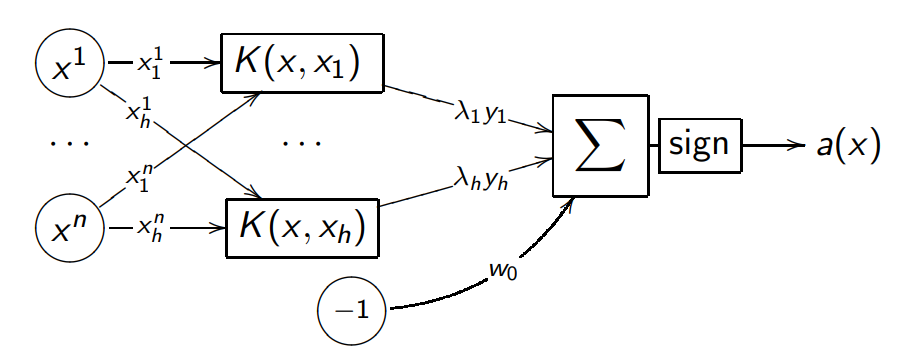
\includegraphics[width=0.8\linewidth]{chapters/svm/images/SVM_neuron.png}
  \caption{SVM в виде двухслойной нейросети}
  \label{fig:mpr}
\end{figure}

    \clearpage
    \chapter{Метод главных компонент}
    \section{Введение в метод главных компонент(PCA)}
\textbf{Метод главных компонент (Principal Component Analysis, PCA)} — это статистический метод, используемый для снижения размерности данных с сохранением наиболее значимой информации. PCA находит новые признаки (главные компоненты), 
которые представляют собой линейные комбинации исходных признаков, причем эти компоненты ортогональны и ранжированы по величине объясняемой дисперсии.
\textbf{Основные этапы метода:} \\
1. \textbf{Центрирование данных}:\\ Данные центрируются так, чтобы среднее значение каждой переменной было равно нулю:
$$
X_c=X-\bar{X},
$$
где $X$ - исходная матрица данных (размер $n \times p$ ), $\bar{X}$ - вектор средних значений по столбцам.\\
2. \textbf{Построение ковариационной матрицы}: \\ Вычисляется ковариационная матрица:
$$
\Sigma=\frac{1}{n-1} X_c^T X_c
$$
где $\Sigma$ - симметричная матрица размером $p \times p$.\\
3. \textbf{Собственные значения и собственные векторы}: \\ Решается задача нахождения собственных значений и собственных векторов ковариационной матрицы:
$$
\Sigma \mathbf{v}_i=\lambda_i \mathbf{v}_i
$$
где $\lambda_i$ - собственные значения, $\mathbf{v}_i$ - соответствующие им собственные векторы.\\
4. \textbf{Ранжирование главных компонент}: \\ Собственные значения упорядочиваются по убыванию:
$$
\lambda_1 \geq \lambda_2 \geq \cdots \geq \lambda_p
$$
Первые несколько компонент, соответствующие самым большим собственным значениям, объясняют большую часть дисперсии данных.\\
5. \textbf{Проекция данных}: \\ Данные проецируются на главные компоненты:
$$
Z=X_c V_k,
$$
где $V_k$ — матрица $k$ собственных векторов, соответствующих $k$ наибольшим собственным значениям, $Z$ — матрица данных в пространстве главных компонент.

Свойства метода: \\
- Главные компоненты ортогональны:

$$
\mathbf{v}_i^T \mathbf{v}_j=0, \quad i \neq j
$$

- Дисперсия объясняется последовательностью собственных значений:

$$
\text { Объясненная дисперсия }=\frac{\sum_{i=1}^k \lambda_i}{\sum_{i=1}^p \lambda_i} \text {. }
$$

\section{Задачи на использование метода главных компонент}

\subsection{Задача 1: Вклад признаков в главные компоненты}
Пусть $X \in R_{n\times p}$ набор данных с n образцами (строками) и p признаками (столбцами). PCA стремится найти набор собственных векторов (главных компонент), которые максимизируют дисперсию данных при проецировании на эти векторы.

Задача состоит в том, чтобы математически оценить, какой вклад вносит каждый признак в главные компоненты, и проранжировать признаки в зависимости от их вклада.\\ \\
\textbf{Решение:}
Метод РСА ищет собственные векторы $\mathbf{v}_i$ и собственные значения $\lambda_i$ удовлетворяющие:

$$
\Sigma \mathbf{v}_i=\lambda_i \mathbf{v}_i,
$$


где $\lambda_i$ - величина дисперсии данных вдоль $\mathbf{v}_i$.
Собственные векторы $\mathbf{v}_i$ формируют матрицу $V=\left[\mathbf{v}_1, \mathbf{v}_2, \ldots, \mathbf{v}_p\right]$, где каждый столбец $\mathbf{v}_i$ указывает направления главных компонент.\\
\textbf{Вклад признака в главные компоненты:}\\

Каждый признак в $X$ вносит вклад в главные компоненты через веса собственных векторов $\mathbf{v}_i$ . Элементы $v_{i j}$ (где $v_{i j}-j$-й элемент $i$-го собственного вектора) определяют значимость $j$-го признака для $i$-й главной компоненты.

Вклад $j$-го признака в $i$-ю главную компоненту оценивается как квадрат соответствующего элемента $v_{i j}^2$ .\\

Общий вклад $j$-го признака во все главные компоненты можно найти, суммируя его взвешенные вклады с учётом дисперсий ( $\lambda_i$ ):\\
$j=\sum_{i=1}^p \lambda_i v_{i j}^2$.\\
Этот показатель учитывает как значимость признака для каждой компоненты $\left(v_{i j}^2\right)$, так и долю дисперсии, объясняемую компонентой ( $\lambda_i$ ).\\
На конкретном примере:
Пусть собственные вектора образуют матрицу V:

$$
V=\left[\begin{array}{cccc}
0.5 & 0.6 & 0.3 & 0.1 \\
0.4 & -0.7 & 0.2 & 0.5 \\
-0.6 & 0.2 & 0.7 & -0.4 \\
0.5 & 0.3 & -0.6 & -0.6
\end{array}\right]
$$
Собственные значения:

$$
\Lambda=\operatorname{diag}(4.0,2.5,1.2,0.3)
$$

Посчитаем вклад признака $1(j=1)$ :
Для этого берём первую строчку $V$ :

$$
v_{1, \cdot}=[0.5,0.6,0.3,0.1]
$$
Считаем:

$$
\begin{aligned}
\text { Contribution }_1 & =\left(0.5^2 \cdot 4.0\right)+\left(0.6^2 \cdot 2.5\right)+\left(0.3^2 \cdot 1.2\right)+\left(0.1^2 \cdot 0.3\right) \\
& =1.0+0.9+0.108+0.003=2.011
\end{aligned}
$$

То же самое повторяем для остальных строк и находим максимальное значение.
\subsection{Задача 2: Ошибка "реконструкции" PCA}
Пусть $X \in R_{n\times p}$ набор данных с $n$ образцами (строками) и $p$ признаками (столбцами), с помощью метода главных компонент нужно:
\begin{itemize}
\item{Спроецируйте данные в более низкоразмерное пространство, определяемое $k$ главными компонентами.}
\item {Реконструируйте исходные данные из пространства пониженной размерности.}
\item {Вычислите ошибку реконструкции и оцените, как она меняется в зависимости от количества сохраняемых компонент k.}
\end{itemize}
\textbf{Решение:}
Для реконструкции данных из $k$-мерного подпространства используется обратная проекция:

$$
\hat{X}=Z V_k^T+\bar{X}
$$


Здесь:
- $Z V_k^T$ возвращает проекцию данных в исходное $p$-мерное пространство.\\
- Добавление $\bar{X}$ восстанавливает исходное смещение данных. \\
Ошибка реконструкции должна показывать какую часть информации мы потеряли при использовании только $k$ компонент при репрезентации данных.\\
1. Определим ошибку реконструкции для одного объекта $x_i$ :

$$
E_i=\left\|x_i-\hat{x}_i\right\|^2=\left\|\left(x_i-\bar{X}\right)-\left(z_i V_k^{\top}\right)\right\|^2
$$

2. Обобщим на весь набор данных:

$$
E=\frac{1}{n \times p} \sum_{i=1}^n\left\|x_i-\hat{x}_i\right\|^2
$$

3. Заменим на выражение для $\hat{x}_i$:

$$
E=\frac{1}{n \times p} \sum_{i=1}^n\left\|x_i-\bar{X}-Z V_k^{\top}\right\|^2
$$
Мы получили выражение для ошибки реконструкции. Теперь докажем, что 
ошибка реконструкции $E$ уменьшается монотонно с $k$, и когда $k=p, E=0$.

1. Общая дисперсия данных - это след ковариационной матрицы, которая представляет собой сумму всех собственных значений:

$$
\text { Total Variance }=\sum_{j=1}^p \lambda_j
$$

2. Дисперсия, которую уловили $k$ компонент это:

$$
\text { Captured Variance }=\sum_{j=1}^k \lambda_j
$$

3. Ошибка реконструкции по сути является дисперсией, которую не удалось уловить, то есть просто:

$$
E=\text { Total Variance }- \text { Captured Variance }=\sum_{j=k+1}^p \lambda_j
$$

4. Так как $\lambda_1 \geq \lambda_2 \geq \cdots \geq \lambda_p \geq 0$, добавление большего числа компонент ( $k \rightarrow k+1$ ) уменьшает $E$ :

$$
\sum_{j=k+1}^p \lambda_j>\sum_{j=k+2}^p \lambda_j
$$

5. В тот момент, когда $k=p, \sum_{j=k+1}^p \lambda_j=0$ $\Rightarrow$ $E=0$.

\subsection{Задача 3: Построить критерий D-оптимальности для выбора лучшиз k-компонент }
Набор данных представляет собой матрицу $n \times p$, где n - число образцов (строк), а p - число признаков (столбцов). Введём критерий D-оптимальности, используемый для выбора подмножества точек из набора данных, которое максимизирует детерминант информационной матрицы.
$$
D_{opt} : max  det(X^{T}X)
$$

Ключевым свойством критерия D-оптимальности является то, что он максимизирует объём многомерной фигуры, которая получается из рассматриваемых признаков. \\
Нужно построить критерий D-оптимальности для выбора лучших 
k главных компонент, которые максимизируют детерминант объясненной дисперсии (или объём фигуры) в k-мерном подпространстве PCA. 

\textbf{Решение:}

Критерий D-оптимальности для подпространства $k$ задаётся максимизацией детерминанта информационной матрицы $\Lambda_k$ :

$$
D_{o p t}(k)=\max \operatorname{det}\left(\Lambda_k\right)
$$

Так как $\Lambda_k$ является диагональной матрицей, её детерминант равен произведению собственных значений:

$$
\operatorname{det}\left(\Lambda_k\right)=\prod_{i=1}^k \lambda_i
$$

Итак, наша задача сводится к выбору $k$-мерного подпространства (т.е. первых $k$ главных компонент), которые максимизируют произведение $\lambda_1 \cdot \lambda_2 \cdots \cdot \lambda_k$, что эквивалентно решению следующей задачи:

$$
\max _{V_k} \prod_{i=1}^k \lambda_i
$$


где $\lambda_i$ - собственные значения матрицы ковариации $\Sigma$.
Для вычисления $D_{\text {opt }}(k)$ :\\
\\
1. Центрируем данные:

$$
X_c=X-\bar{X},
$$


где $\bar{X}$ - матрица средних значений.\\
2. Вычисляем ковариационную матрицу:

$$
\Sigma=\frac{1}{n-1} X_c^T X_c
$$

3. Находим собственные значения $\lambda_1, \lambda_2, \ldots, \lambda_p$ и соответствующие собственные векторы $\mathbf{v}_1, \mathbf{v}_2, \ldots, \mathbf{v}_p$.\\
4. Выбираем первые $k$ собственных значений $\lambda_1, \lambda_2, \ldots, \lambda_k$, которые максимизируют:

$$
\prod_{i=1}^k \lambda_i
$$

Максимизация $\prod_{i=1}^k \lambda_i$ эквивалентна максимизации объёма \textbf{$k$-мерного эллипсоида}, описывающего данные в пространстве первых $k$ главных компонент. Это позволяет отобрать $k$ измерений, которые сохраняют максимальную дисперсию данных.


\section{Денойзинг данных с помощью метода главных компонент}
Метод главных компонент (PCA) — это один из самых распространенных и эффективных методов для снижения размерности данных, который также может быть применен для денойзинга. Денойзинг данных — это процесс удаления шума из наблюдений для выделения более чистых и значимых сигналов. Во многих областях, таких как обработка изображений, анализ звука, необходимо избавляться от шумов, которые могут искажать результаты анализа и ухудшать качество моделей.

Благодаря своей способности выявлять скрытые структуры в многомерных данных PCA может быть использован для денойзинга. При анализе данных PCA проецирует данные в пространство главных компонент. 

Основные моменты применения PCA для денойзинга включают:
\begin{itemize}
\item Выделение главных компонент: 
PCA позволяет выделить компоненты, вдоль которых данные наиболее рассеяны.

\item Реконструкция данных: Уменьшение уровня шума и восстановление более "чистого" сигнала могут быть произведены с помощью удаления компонент, у которых меньше дисперсия. 

\item Снижение размерности: PCA снижает размерность данных, что делает их более вычислительно эффективными. Это особенно полезно в контексте обработки больших объемов данных.
\end{itemize}

PCA выбирают по следующим причинам:
\begin{itemize}
\item Линейность: PCA представляет собой линейный метод, что делает его простым для интерпретации и анализа. Однако основной недостаток заключается в том, что он может не эффективно обрабатывать данные с нелинейными взаимосвязями.

\item Простота реализации: PCA является относительно простым в реализации. Многие библиотеки для анализа данных, такие как scikit-learn в Python, имеют встроенные инструменты для выполнения PCA.

\item Характеристики контекста: PCA позволяет не только проводить денойзинг, но и выявлять основные характеристики и структуры в данных, что часто полезно при анализе образцов.
\end{itemize}

PCA может значительно упростить сложные многомерные наборы данных, обеспечивая при этом сохранение наиболее важной информации. При этом снижение размерности данных может помочь в построении более легких и интерпретируемых моделей, что особенно важно в машинном обучении.
Однако у PCA есть и минусы. Так, отбрасывание компонент может привести к потере важной информации, если не удается точно оценить, какие компоненты следует сохранять. Ограниченность линейности также может быть недостатком, так как в данных со сложными и нелинейными зависимостями PCA может не обнаружить все важные структуры. Хотя PCA упрощает данные, интерпретировать полученные главные компоненты может быть непросто, поскольку они являются линейными комбинациями исходных переменных.

Таким образом, метод главных компонент является мощным инструментом для денойзинга данных, особенно в контексте многомерных наборов данных. Его способность выявлять значимую информацию и удалять шум делает его предпочтительным выбором в различных областях. Однако важно учитывать плюсы и минусы метода, чтобы правильно применять его в соответствии с конкретными задачами и свойствами данных. Выбор подходящего количества компонент и тщательная интерпретация результатов остаются ключевыми шагами, которые могут существенно повлиять на успех применения PCA для денойзинга.

\section{Задачи про денойзинг данных}
\textbf{Задача 1}\\
Пусть \( I \) — это набор изображений, состоящий из \( n \) изображений, каждое из которых имеет \( m \) пикселей. Изображения могут содержать шум, например, из-за помех во время съемки. Требуется устранить этот шум, сохраняя основные детали изображения с помощью PCA.

\underline{Решение:}
Данные можно представить в виде матрицы \( X \in \mathbb{R}^{n \times m} \), где строки соответствуют изображениям, а столбцы — пикселям. Далее необходимо центрировать данные, вычитая среднее значение по каждому столбцу (пикселю):
   \[
   X_{cen} = X - \mu
   \]
   где \( \mu \) — вектор среднего значения по всем изображениям.
Вычислим ковариационную матрицу:
   \[
   C = \frac{1}{n-1} X_{cen}^T X_{cen}
   \]
Далее необходимо найти собственные значения \( \lambda_i \) и собственные векторы \( v_i \) матрицы \( C \) и упорядочить собственные значения по убыванию. Отберем первые \( k \) собственных векторов, которые обеспечивают максимальную дисперсию, где \( k \) выбирается в зависимости от дисперсии. Запишем выбранные векторы в матрицу \( V_k \).
Спроектируем центрированные данные на выбранные главные компоненты:
   \[
   Z = X_{cen} V_k.
   \]
Реконструируем уменьшенную версию изображений, используя только \( k \) основных компонент:
   \[
   \hat{X} = Z V_k^T + \mu.
   \]

\textbf{Задача 2}\\
Пусть \( D \) --- оригинальные данные, которые содержат как полезную информацию, так и шум. После применения PCA к данным были получены очищенные данные (денойзинг) \( D' \). Оценить, насколько эффективно PCA справилось с устранением шума, используя метрику RMSE (Root Mean Square Error, RMSE).

\underline{Решение:}
Вычислим разницу (ошибку) между оригинальными и очищенными данными:
   \[
   E_{i} = D_{i} - D'_{i}, \quad \forall i = 1, 2, \ldots, n
   \]
Затем вычисляем RMSE для получения общих значений ошибок:
   \[
   RMSE = \sqrt{\frac{1}{n} \sum_{i=1}^{n} E_{i}^2} = \sqrt{\frac{1}{n} \sum_{i=1}^{n} (D_{i} - D'_{i})^2}
   \]

\textbf{Задача 3}\\
Пусть \( D \) --- оригинальные данные, которые содержат как полезную информацию, так и шум. После применения PCA к данным были получены очищенные данные (денойзинг) \( D' \). Оценить, насколько эффективно PCA справилось с устранением шума, используя коэффициент детерминации\( R^2 \).

\underline{Решение:}
   \[
   R^2 = 1 - \frac{\sum_{i=1}^{n} (D_{i} - D'_{i})^2}{\sum_{i=1}^{n} (D_{i} - \bar{D})^2}
   \]
   где \( \bar{D} \) — среднее значение оригинальных данных.

\end{document}

\section{Оценка оптимального числа главных компонент}
\subsection{Определение и идея метода}
PCA — это статистический метод, который позволяет сократить размерность данных, сохраняя при этом наибольшее количество информации. Главная идея PCA заключается в том, чтобы найти новые признаки, называемые главными компонентами, которые максимально коррелируют с исходными данными.\\

Математическое содержание метода главных компонент — это спектральное разложение ковариационной матрицы $\displaystyle C$, то есть представление пространства данных в виде суммы взаимно ортогональных собственных подпространств
$\displaystyle C$, а самой матрицы $\displaystyle C$ — в виде линейной комбинации ортогональных проекторов на эти подпространства с коэффициентами собственных значений $\displaystyle \lambda _{i}$. Если $X = \{x_{1}, ... ,x_{m}\}^{T}$  — матрица, составленная из векторов-строк центрированных данных, то $\displaystyle C =\frac {1}{m-1} X ^{T} X$

\\

\subsection{Почему важна оценка числа главных компонент?}
Оптимальное число главных компонент имеет большое значение, так как оно влияет на качество модели, интерпретацию результатов и общую эффективность анализа. Если число компонент слишком велико, это может привести к избыточности и переобучению, в то время как слишком малое число компонент может привести к потере важной информации.

\subsection{Сколько главных компонент необходимо?}

Не существует общепринятого объективного способа определить оптимальное число главных компонент. На самом деле, вопрос зависит от конкретной области применения и конкретного набора данных. Однако существуют подходы, которые могут служить руководством для ответа на этот вопрос.

\subsubsection{Метод объясненной дисперсии}
Этот метод заключается в выборе числа компонент так, чтобы доля объясненной дисперсии достигла заданного порога (например, 95\% или 99\%). Это позволяет сохранить большую часть информации при снижении размерности.

\subsubsection{Критерий Кайзера-Гуттмана}
Согласно правилу Кайзера, собственное значение главной компоненты больше 1 указывает на то, что компонента объясняет больше дисперсии, чем среднее значение одной переменной. Таким образом, компоненты с собственными значениями менее 1 не стоит сохранять, так как они приносят мало полезной информации. Иными словами значимы те главные компоненты, для которых $\displaystyle \lambda _{i}>\frac {1}{n} tr C$ то есть 
$\displaystyle \lambda _{i}$ превосходит среднее значение 
$ \displaystyle \lambda$ (среднюю выборочную дисперсию координат вектора данных). Правило Кайзера хорошо работает в простых случаях, когда есть несколько главных компонент с 
$\displaystyle \lambda _{i}$, намного превосходящими среднее значение, а остальные собственные числа меньше него. В более сложных случаях оно может давать слишком много значимых главных компонент. 

\subsubsection{Правило сломанной трости}
Набор нормированных на единичную сумму собственных чисел $(\displaystyle \lambda _{i}/ tr C, i = 1, ... ,n)$ сравнивается с распределением длин обломков трости единичной длины, ломанной в n − 1-й случайно выбранной точке (точки разлома выбираются независимо и равнораспределены по длине трости).

По правилу сломанной трости k-й собственный вектор (в порядке убывания собственных чисел $\lambda _{i}$ сохраняется в списке главных компонент, если $\frac {\lambda _{1}}{tr C} >l_{1}$

Говоря про визуальный анализ, этот метод часто упрощают до так называемого метода "локтя". Мы строим график, где по оси X отложено число компонент, а по оси Y - доля объясненной дисперсии. График будет иметь форму локтя, и точка, где снижение доли объясненной дисперсии замедляется, будет сильно приближенно указывать на оптимальное число компонент.

\subsection{Задачи}
\subsubsection*{Задача 1.}

У вас есть выборка из 50 объектов с 5 признаками, результаты анализа главных компонент: собственные значения 5.0, 2.0, 1.0, 0.5, 0.3. Какое минимальное количество компонент нужно выбрать, чтобы объяснить не менее 90\% дисперсии?

\begin{solution}
    Сумма собственных значений - 8.8. 90\% суммы = 7.92.
    
    5.0 + 2.0 = 7.0 (менее 90\%) - не достаточно

    5.0 + 2.0 + 1.0 = 8.0 (больше 90\%) - оптимальное число главных компонент 3 
\end{solution}
\subsubsection*{Задача 2.}

Предположим, что у нас есть 2 разных датасета с 4 признаками. Первый содержит информацию об жителях окраинного района типичного для страны N города. А именно уровне доходов, жилой площади, количестве топлива, покупаемого за месяц, и числе домашних животных на каждого жителя. Второй датасет - признаки, относящиеся к производительн работников какой-либо сферы: количество выходных часов, число сотрудников в группе, температура в помещении и время, провиденное за монитором. В каком из этих случаев вероятно ожидать, что оценка главных компонент будет нереалистичной и почему?  

\begin{solution}
    Скорее всего, в первом датасете при оценке главных компонент мы столкнемся с переоценкой их числа. Так как наши фичи достаточно схожие, все связаны с уровнем дохода, и, веротно, будет мультиколлинеарность в данных. Второе, так как это жители одного района какого-то типичного города возможно дисперсия каждой фичи будет низкой и значение каждого собственного числа будет низким.
\end{solution}


    \clearpage
    \chapter{Нелинейные модели машинного обучения}
    \section*{Методы Ньютона-Рафсона, Ньютона-Гаусса}

Мы уже познакомились с задачами линейной регрессии и обсудили несколько методов их решения. Но что делать если задача нелинейна? Оказывается, что идея локальной линейности гладкой функций позволяет свести задачу к более простому. На этой идее основаны методы второго порядка - Ньютона-Рафсона и Ньютона-Гаусса.

\subsection*{Метод Ньютона-Рафсона}

Начнем немного сдалека, а именно рассмотрим задачу поиска нуля $a$ функций $f(x)$. Пусть мы находимся в точке $a^{0}$ и хотим найти такое приращение $h$, чтобы приблизиться к точке $a$: $a^{0} + h \approx a$. Применим разложение в ряд:

\begin{gather*}
    f(a^{0} + h) = f(a^{0}) + f'(a^{0})h + o(h)\\[1em]
    f(a^{0} + h) \approx f(a) = 0 \Rightarrow f(a^{0}) + f'(a^{0})h \approx 0
\end{gather*}

Откуда

\[
h \approx - \frac{f(a^{0})}{f'(a^{0})}
\]

Значит, для поиска нуля выпуклой функций \( f \) можно применить следующий итеративный метод:

\[
a^{k + 1} = a^{k} - \frac{f(a^{k})}{f'(a^k)}
\]

Вернемся к начальной задаче:

\begin{itemize}
    \item обучающая выборка \( X^{l} = (x_{i}, y_{i}) \), где \( x_{i} \) - вектор признаков \( i \)-го объекта
    \item \( y_{i} = y(x_{i}),\quad y: X \to Y \) - неизвестная регрессионная зависимость
    \item \( f(x, \alpha) \) - нелинейная модель регрессии, где \( \alpha \) - вектор параметров
\end{itemize}

Хотим решить задачу оптимизации методом наименьших квадратов:

\[
Q(\alpha, X^{l}) = \sum\limits_{i = 1}^{l}\left(f(x_{i}, \alpha) - y_{i} \right)^{2} \to \min_{\alpha}
\]

Функция потерь \( Q(\alpha, X^{l}) \) выпукла и гладкая в предположений гладкости \( f(\alpha, x) \), поэтому для ее минимизаций достаточно найти нуль производной (градиента). Применяя рассуждения выше и опустив технические детали, получим следующий итерационный процесс:

\[
\alpha^{k + 1} = \alpha^{k} - h_{k}\left(Q''( \alpha^{k} )\right)^{-1} Q'(\alpha^{k})
\]

где \( Q'( \alpha^{k} ) \), \( Q''(\alpha^{k} ) \) - градиент и гессиан \( Q \) в точке \( \alpha^{k} \) соответственно, \( h_{k} \) - величина шага.
\subsection*{Метод Ньютона-Гаусса}

Подсчет обратного гессиана на каждой итерации может дорого обходиться, поэтому посмотрим на полученный выше результат с другой стороны. Для этого запишем несколько формул:

Компоненты градиента \( Q(\alpha, X^{l}) \):

\[
\frac{\partial Q(\alpha, X^{l})}{\partial\alpha_{j}} = 2 \sum\limits_{i = 1}^{l} \left(f(x_{i}, \alpha) - y_{i} \right)\frac{\partial f(x_{i}, \alpha)}{\partial\alpha_{j}}
\]

Компоненты гессиана:

\[
\frac{\partial Q(\alpha, X^{l})}{\partial\alpha_{j}\partial\alpha_{k}} = 2\sum\limits_{i = 1}^{l}\frac{\partial f(x_{i}, \alpha)}{\partial\alpha_{j}}\frac{\partial f(x_{i}, \alpha)}{\partial\alpha_{k}} - 2\sum\limits_{i = 1}^{l}\left(f(x_{i}, \alpha) - y_{i}\right)\frac{\partial^2 f(x_{i}, \alpha)}{\partial\alpha_{j}\partial\alpha_{k}}
\]

Второе слагаемое в формуле выше полагается равным нулю, исходя из линейной аппроксимации функций \( f \). Введем следующие обозначения и перепишем формулу итерации метода Ньютона-Рафсона:

\begin{gather*}
    F_{k} = \left( \frac{\partial f}{\partial\alpha_{j}}(x_{i}, \alpha^{k}) \right)_{i, j}\\[1em]
    f_{k} = \left( f(x_{i}, \alpha^{k}) \right)_{i}
\end{gather*}

Получим:

\[
\alpha^{k + 1} = \alpha^{k} - h_{k}(F_{k}^{T}F_{k})^{-1}F_{k}^{T}(f_{k} - y)
\]

Положив \( \theta = (F_{k}^{T}F_{k})^{-1}F_{k}^{T}(f_{k} - y) \), получим решение задачи линейной регрессии, где новые ответы обучающей выборки -- \( \left(f_{k} - y \right) \), с новой матрицей признаков~--~\( F_{k} \). Таким образом, каждый шаг метода Ньютона-Гаусса сводится к задаче линейной регрессии. 

\section*{Задачи}

\subsection*{Задача 1: Локальная сходимость}

Найдите допустимые значения начального приближения для поиска нуля функции \( f(x) = \frac{x}{\sqrt{1 + x^{2}}} \).

\textbf{Решение:}

Нуль функции \( f \) достигается в точке \( a = 0\). Посчитаем производную \( f \):

\[
f'(x) = \left(\frac{x}{\sqrt{1 + x^{2}}}\right)' = \frac{1}{\sqrt{1 + x^{2}}} - x\cdot\frac{2x}{2(1 + x^{2})^{3/2}} = \frac{1}{(1 + x^{2})^{3/2}}
\]

Распишем формулу итерации метода Ньютона:

\[
a^{k + 1} = a^{k} - \frac{f(a^{k})}{f'(a^{k})} = -(a^{k})^3
\]

Отсюда видно, что сходимость есть при \( |a^{0}| < 1 \). Делаем вывод о важности выбора начального приближения в данном методе.

\subsection*{Задача 2: Квадратичная задача}

Как сработает метод Ньютона-Рафсона для поиска минимума задачи \( f(x)~=~x^{T}Ax + bx + c\),  где $x, b \in \mathbb{R}^{n}$, $A$ - симметричная, положительно определенная матрица.

\textbf{Решение:}

Для поиска минимума нужно найти нуль градиента. Это и будет точкой минимума, так как задача выпукла.
Посчитаем градиент и гессиан:

\begin{gather*}
    \nabla f(x) = Ax + b\\[1em]
    \nabla^{2} f(x) = A
\end{gather*}

Пусть \( x^{0} \) начальная точка. Применяя формулу из метода Ньютона-Рафсона получим:

\[
x^{1} = x^{0} - \left(\nabla^{2} f(x^{0})\right)^{-1}\nabla f(x^{0}) = x^{0} - A^{-1}\left(Ax^{0} + b\right) = -A^{-1}b
\]

но с другой стороны, градиент обращается в нуль в этой точке:

\[
\nabla f(x) = 0 = Ax + b \Rightarrow x = -A^{-1}b
\]


Значит для квадратичной задачи данный метод дает ответ за 1 шаг. Вообще говоря, если функция $\mu$-выпукла и имеет $M$-липшецевый гессиан, то скорость сходимости локально квадратична.

\subsection*{Задача 3: Система уравнений}

Составьте алгоритм решения следующей системы с помощью методов второго порядка:

\[
\begin{cases}
x^{2} + y^{2} = 4\\
y = e^{x}
\end{cases}
\]

\textbf{Решение:}

Нужно найти нули следующей функции от двух переменных
\[
F(x, y) = 
\begin{pmatrix}
x^{2} + y^{2} - 4 \\
y - e^x
\end{pmatrix}
\]

Запишем итерацию метода Ньютона-Рафсона:

\[
x^{k + 1} = x^{k} - J_{F}(x^{k})^{-1}F(x^{k})
\]

Его можно записать как:

\[
J_{F}(x^{k})(x^{k + 1} - x^{k}) = -F(x^{k})
\]

Посчитаем матрицу якоби функции $F$:

\[
J_{F}(x) = 
\begin{pmatrix}
2x   & 2y \\
-e^x & 1
\end{pmatrix}
\]

Тогда на каждом шаге нужно решить следующую систему:
\[
\begin{pmatrix}
    2x^{k} & 2(y^{k})^{2} \\
    -e^{x^{k}} & 1 
\end{pmatrix}
\begin{pmatrix}
    c_{1}^{k + 1}  \\
    c_{2}^{k + 1}
\end{pmatrix} 
=
\begin{pmatrix}
    (x^{k})^2 + (y^{k})^2 - 4\\
    (y^{k}) - e^{x^{k}}
\end{pmatrix} 
\]

где \( c^{k + 1} = -(x^{k + 1} - x^{k})\). Тогда для решения данной задачи нужно взять начальную точку и проделать несколько итераций описанных уравнениями выше.

\section{Backfitting}

На практике встречаются задачи, в которых использование линейных моделей необосновано, но и не удаётся предложить явную нелинейную модель. В таком случае строится модель вида

$$\displaystyle y(x)=f(x,\theta)=\sum_{j=1}^m\theta_j \phi_j(x_j),$$

где $x$ ~--- объект, $x_j$ ~--- признаки объекта, $\phi_j:\mathbb{R}\rightarrow \mathbb{R}$ ~--- нелинейные в общем случае преобразования.

Задача состоит в том, чтобы одновременно подбирать коэффициенты модели $\theta_j$ и неизвестные преобразования $\phi_j$.

Суть метода backfitting (метод настройки с возвращением) заключается в чередовании оптимизации коэффициентов $\theta_j$ при постоянных $\phi_j$ методами линейной регрессии, и оптимизации преобразований $\phi_j$ при постоянных коэффициентах $\theta_j$. 

Для минимизации используется сумма квадратов ошибок на всех объектах:

$Q(\theta, \phi) = \displaystyle \sum_{i=1}^l \left( y(x_i) - y_i \right)^2 = \sum_{i=1}^l \left( \sum_{j=1}^m \theta_j \phi_j(X_{ij}) - y_i \right)^2 $

Здесь $X$ ~--- матрица признаков.

\subsection{Алгоритм backfitting}
\begin{algorithmic}
\State $\phi_j(t) \equiv t$ ~--- изначальное приближение линейными функциями
\While{($Q$ уменьшается)} 
    \State $\theta \gets \text{argmin}_{\theta}Q(\theta, \phi_j)$ ~--- при фиксированных $\phi_1,\dots, \phi_k$
    \For{$j=1\dots m$}
        \State $\displaystyle r_i = y_i - \sum_{k\neq j} \theta_k \phi_k(X_{ik})$
        \State $r_i$ ~--- ошибка модели на $i$ объекте, без учёта $j$ признака
        \State $\displaystyle\phi_j \gets \text{argmin}_{\phi} \sum_{i=1}^l \left( \theta_j \phi(X_{ij}) - r_i \right)^2$ ~--- при $\theta_j=const$
    \EndFor
\EndWhile 
\end{algorithmic}

Оптимизация по коэффициентам $\theta \gets \text{argmin}_{\theta}Q(\theta, \phi_j)$ выполняется методами линейной регрессии, такими как стохастический градиентный спуск.

Оптимизация по функции $\phi_j$ выполняется одномерными методами, такими как ядерное сглаживание.

Варианты дальнейшего развития метода:
\begin{itemize}
    \item [1.] Во внутреннем цикле выбирать индексы $j$ не в фиксированном порядке, а в первую очередь оптимизировать дающие наибольший вклад в $Q$.
    \item [2.] Регуляризация $Q$ по параметрам $\theta$ и по сложности функций $\phi$.
\end{itemize}

\subsection{Задача}

Если матрица признаков $X$ разреженная, с какой проблемой можно столкнуться, применяя алгоритм backfitting, и как её решить?

Решение: если каждая из функций $\phi_j$ вызывается лишь на небольшом наборе аргументов, то её значения на них могут быть почти независимы (если модель $\phi$ достаточно сложна, например, полином высокого порядка), и случится переобучение. Варианты решения: большая константа регуляризации по сложности функций $\phi$; ограничить $\phi$ более простым классом функций (например, только квадратичные функции вместо полиномов); расширить матрицу признаков несколькими простыми нелийными преобразованиями ($\sin x$, $x^2$...) и использовать методы линейной регрессии.


    \clearpage
    \chapter{Обобщенные линейные модели}
    \section*{Lasso-регрессия (L1-регуляризация)}

Lasso-регрессия (Least Absolute Shrinkage and Selection Operator) включает $\ell_1$-регуляризацию, которая одновременно выполняет отбор признаков и предотвращает переобучение. Задача оптимизации формулируется следующим образом:
\[
\min_{\beta \in \mathbb{R}^p} \frac{1}{2n} \sum_{i=1}^n (y_i - x_i^T \beta)^2 + \lambda \|\beta\|_1,
\]
где $\|\beta\|_1 = \sum_{j=1}^p |\beta_j|$, а $\lambda > 0$ — параметр регуляризации. Штраф $\ell_1$ приводит к занулению некоторых коэффициентов $\beta_j$, тем самым автоматически выполняя отбор признаков.

\subsection*{Задача 1}
Как на основе Lasso-регрессии определить значимость признаков в линейной модели? 

\subsection*{Задача 2}
Сохраняет ли L1-регуляризация следующие свойства оптимизационной задачи:
\begin{itemize}
    \item гладкость,
    \item выпуклость,
    \item сильную выпуклость?
\end{itemize}

\subsection*{Задача 3}
Как известно, метод SVM сводится к решению задачи квадратичного программирования. Сохраняет ли эта задача квадратичность при добавлении L1-регуляризации? Если нет, какие методы оптимизации можно использовать для эффективного решения этой задачи?


    \clearpage
    \chapter{Нестандартные функции потерь}
    \section*{Нестандартные функции потерь. Метод наименьших модулей. Квант\'{и}льная регрессия.}

Квадратичная функция потерь обычно дает хорошие результаты, является удобной в использовании, а потому и применяется чаще всего. Но в некоторых ситуациях она все же неприменима, и приходится использовать нестандартные функции потерь.

\subsection*{Метод наименьших модулей.}

Здесь и далее будем использовать следующие обозначения: $\ell$ - количество объектов в тренировочной выборке, $x_i$ ($i \in \left\{1, \dotsc, \ell \right\}$) - вектор признаков, $y_i$ ($i \in \left\{1, \dotsc, \ell \right\}$) - таргет, $a$ - модель, $\varepsilon_i := a(x_i) - y_i$ ($i \in \left\{1, \dotsc, \ell \right\}$).

Для стандартной квадратичной функции потерь $\mathscr{L}(\varepsilon) = \varepsilon^2$ задача будет выглядеть так:
$$\frac{1}{\ell}\sum\limits_{i=1}^\ell\left(a(x_i) - y_i\right)^2 \longrightarrow \min\limits_{a}.$$

Заменим функцию потерь на $\mathscr{L}(\varepsilon) = |\varepsilon|$.
Задача станет выглядеть так:
$$\frac{1}{\ell}\sum\limits_{i=1}^\ell\left|a(x_i) - y_i\right| \longrightarrow \min\limits_{a}.$$
Данный метод называется \textit{методом наименьших модулей}.

В какой ситуации такой подход может оказаться полезным? Рассмотрим ситуацию,  когда наша модель - это константа, то есть она вообще не зависит от признаков. Для квадратичной функции потерь получим:
$$\frac{1}{\ell}\sum\limits_{i=1}^\ell\left(a - y_i\right)^2 \longrightarrow \min\limits_{a}.$$
Здесь можно посчитать ответ аналитически, оптимальной константой $a$ будет $a = \frac{1}{\ell}\sum\limits_{i=1}^\ell y_i$, то есть среднее арифметическое таргетов. Это плохая оценка, если, например, в нашей выборке присутствуют выбросы, или распределение ошибок имеет тяжёлые <<хвосты>>.

А в случае использования метода наименьших модулей задача будет выглядеть так:
$$\frac{1}{\ell}\sum\limits_{i=1}^\ell\left|a - y_i\right| \longrightarrow \min\limits_{a}.$$
Здесь опять же можно посчитать ответ аналитически, оптимальным $a$ будет $a = \median\left\{ y_1, \dotsc, y_\ell \right\} = y_{(\ell / 2)}$ (серединный член вариационного ряда). Эта оценка хороша тем, что устойчива к выбросам, хорошо работает для распределений ошибок с тяжелыми <<хвостами>>.

Таким образом, использование метода наименьших модулей в некоторых ситуациях помогает бороться с выбросами.

\subsection*{Квант\'{и}льная регрессия.}

Метод наименьших модулей можно обобщить. Давайте по-разному штрафовать отрицательные и положительные ошибки. Т.е. будем рассматривать функцию потерь вида
$$\mathscr{L}(\varepsilon) = \begin{cases}
    C_+|\varepsilon|, \varepsilon \geq 0,\\
    C_-|\varepsilon|, \varepsilon < 0.
\end{cases}$$

\begin{figure}[h]
    \centering
    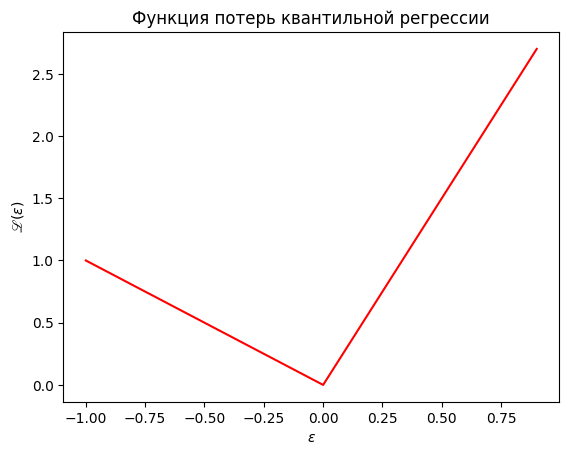
\includegraphics{chapters/nonstandart_error/images/ФПКР.png}
\end{figure}

Опять же рассмотрим случай, когда модель не зависит от признаков, то есть является константой:
$$\frac{1}{\ell}\sum\limits_{i=1}^\ell\mathscr{L}\left(a - y_i\right) \longrightarrow \min\limits_{a}.$$
Решение данной задачи опять же можно получить аналитически, оптимальным $a$ будет $a = y_{(q)}$ ($q$-тый член вариационного ряда), где $q = \frac{\ell C_-}{C_- + C_+}$.
Именно поэтому используемый метод называется \textit{методом квант\'{и}льной регрессии}.

Рассмотрим также еще один случай, когда квантильная регрессия оказывается хорошим вариантом с точки зрения решения задачи оптимизации, а именно случай линейной модели: $a(x) = \left\langle x, w \right\rangle$, где $w$ - вектор весов.

Сделаем замену переменных $\varepsilon_i^+ = (a(x_i) - y_i)_+$, $\varepsilon_i^- = (a(x_i) - y_i)_-$. Тогда наша задача будет иметь вид
$$\begin{cases}
    \frac{1}{\ell}\sum_{i=1}^\ell C_+\varepsilon_i^+ + C_-\varepsilon_i^- \longrightarrow \min\limits_{w},\\
    \left\langle w, x_i \right\rangle - y_i = \varepsilon_i^+ - \varepsilon_i^-, i \in \left\{ 1 , \dotsc, \ell \right\}.
\end{cases}$$

Это задача линейного программирования, для решения которой существует масса способов.

\newpage

\subsection*{Задачи.}

\subsubsection*{Задача 1.}

Предположим, у Вас есть датасет с данными о жителях некоторой страны Южной или Центральной Африки, а также данные об их среднем ежедневном доходе, и Вы хотите научиться предсказывать этот доход по значениям рассматриваемых признаков. Полученная модель в последующем будет использоваться для составления плана по оказанию гуманитарной помощи населению. Что использовать предпочтительнее: квадратичную функцию потерь или функцию потерь квант\'{и}льной регрессии? Почему? Если использовать предпочтительнее функцию потерь квант\'{и}льной регрессии, то каким должно быть соотношение параметров $C_+$ и $C_-$ и почему?

\begin{solution}
    В условии задачи не зря указано, из какого региона у нас страна. Б\'{о}льшая часть населения в ней, скорее всего, крайне бедна, при этом есть очень незначительное количество сверхбогатых людей, т.е., в нашей терминологии, выбросов. Поэтому функция потерь квант\'{и}льной регрессии более предпочтительна, чем квадратичная функция потерь.

    Теперь обратим внимание на то, как будет использована модель, чтобы понять, какая ошибка для нас наиболее страшна: положительная или отрицательная. Заметим, что если мы предсказали доход человека больше реального, т.е. ошибка положительна, то, скорее всего, на него будет выделено меньше помощи. Это кажется более страшным, чем ситуация, в которой мы предсказали доход человека меньше реального, и дали ему чуть больше помощи. Поэтому штрафовать положительные ошибки стоит сильнее, чем отрицательные, то есть стоит выбрать $C_+$ и $C_-$ так, чтобы $C_+/C_- > 1$.
\end{solution}

\subsubsection*{Задача 2.}

Предположим, что у в природе некоторый таргет действительно линейно зависит от вектора признаков, но вектор таргетов, который у нас есть, зашумлен ошбиками, причем ошибки эти приходят из симметричного распределения Коши. Почему использование квадратичной функции потерь в данном случае будет крайне нежелательным? А если ошибки приходит из распределения $\mathcal{N}(a, \sigma^2)$, где $a \neq 0$?

\begin{solution}
    Из теории вероятностей и математической статистики известно, что у распределения Коши тяжелые <<хвосты>>, из-за чего у него даже нет матожидания. Именно поэтому квадратичная функция потерь, очень сильно штрафующая за большие ошибки, здесь не подходит. А вот метод наименьших модулей подхолит лучше.

    Также можно заметить, что квадратичная функция потерь одинаково штрафует положительные и отрицательные ошибки, то есть неявно подразумевается симметричность распределения. В общем случае это не так. Квант\'{и}льная регрессия позволяет более гибко работать с несимметричными распределениями.
\end{solution}

\subsubsection*{Задача 3.}

Предположим, что Вы тестируете новое лекарство на мышах. Вы хотите понять, какая доза лекарства оптимальна: уже вылечивает мышь, но все еще не дает негативных побочных эффектов. Известно, что каждый новый побочный эффект проявляется при превышении некоторого примерно одинакового для всех мышей порога передозировки и действует все сильнее и сильнее при дальнейшем превышении этого порога. Также известно, что оптимум не единственен, а достигается на некотором отрезке, длина которого вам тоже заранее известна. Наконец, ниже некоторого порога лекарство действует все хуже и хуже. У Вас есть некоторые данные о мышах, а также таргеты - максимальные оптимальные дозы лекарств. Предложите модификацию функции потерь квант\'{и}льной регрессии, оптимальную для данной задачи.

\begin{solution}
    Основная идея квант\'{и}льной регрессии по сравнению с методом наименьших модулей состоит в том, что мы по-разному штрафуем положительные и отрицательные ошибки. Давайте разовьем эту идею, и будем по-разному штрафовать ошибки в зависимости от того, в какую часть числовой прямой мы попали.

    Так, для нашей задачи, пусть новые побочные эффекты проявляются при превышении дозировки на $a_1, \dotsc, a_n$ у.е., где $0= a_1 < \ldots < a_n$. А длина оптимального отрезка дозировки равна $b$, Тогда можно взять такую функцию потерь:
    $$\mathscr{L}(\varepsilon) = \begin{cases}
        -v_b\varepsilon, \varepsilon < -b,\\
        0, \varepsilon \in [-b; a_1],\\
        v_{a_1}\varepsilon, \varepsilon \in (a_1; a_2],\\
        (v_{a_1} + v_{a_2})\varepsilon, \varepsilon \in (a_2; a_3],\\
        \vdots\\
        (v_{a_1} + \dotsb + v_{a_{n - 1}})\varepsilon, \varepsilon \in (a_{n-1}; a_n],\\
        (v_{a_1} + \dotsb + v_{a_n})\varepsilon, \varepsilon > a_n,
    \end{cases}$$
    где $v_b, v_{a_1}, \dotsc, v_{a_n}$ - скорости роста соответствующих проблем.
\end{solution}

\newpage
\section*{SVM-Regression}

Регрессионные модели на основе метода опорных векторов (SVM-regression) зачастую используют особую функцию потерь, отличающуюся от стандартной квадратичной ошибки (MSE). В частности, классический SVM для регрессии использует \(\varepsilon\)-insensitive функцию потерь (\(\varepsilon\)-insensitive loss), которая игнорирует ошибки, величина которых меньше заранее заданного порога \(\varepsilon\). Однако существуют и нестандартные функции потерь, которые могут быть полезны в специфических задачах, например, когда необходимо учитывать асимметрию ошибок, различные веса отдельных наблюдений или же более сложные, ориентированные на распределение отклонений, формулы.

Классическая \(\varepsilon\)-insensitive функция потерь:
Для модели вида \(f(x) = \langle w, x \rangle + b\) функция потерь определяется следующим образом:
\begin{align*}
L(\varepsilon) = \max(0, | y - f(x) | - \varepsilon).
\end{align*}

Если \(| y - f(x) | \leq \varepsilon\), то штраф равен нулю, что делает модель нечувствительной к небольшим отклонениям и позволяет контролировать сложность аппроксимации.

Нестандартные функции потерь могут иметь следующие особенности:

\begin{enumerate}
    \item Асимметричные функции потерь: например, более сильное штрафование положительных отклонений, чем отрицательных, или наоборот. Это может быть полезно, если цена переоценки или недооценки целевой переменной различна.
    \item Частично-кусочные функции: использование различных режимов штрафования в зависимости от величины отклонения, например, линейная область штрафа для малых ошибок и квадратичная — для больших.
    \item Функции с весами для разных точек: если некоторые точки обучающей выборки важнее, можно ввести веса и штрафовать ошибки по более значимым точкам сильнее.
    \item Нелинейные преобразования ошибки: например, логарифмическая или экспоненциальная функция потерь, которая меняет чувствительность модели к большим отклонениям.
\end{enumerate}

Пример асимметричной \(\varepsilon\)-insensitive функции потерь:
\begin{align*}
    L(\varepsilon, \alpha) = 
        \begin{cases}
            \case 0, & | y - f(x) | \leq \varepsilon \\
            \case \alpha(y - f(x)) - \varepsilon, & y - f(x) > \varepsilon \\
            \case \frac{(y - f(x))}{\alpha} - \varepsilon, & f(x) - y > \varepsilon
        \end{cases}
\end{align*}
где \(\alpha > 1\) задаёт степень асимметрии штрафования. Такая функция потерь позволит модели сильнее реагировать на недостаточную оценку и слабее —-- на переоценку.

\newpage
\subsection*{Задачи}

\subsubsection*{Задача 1.}
Пусть у нас есть набор точек для регрессии \(\{(x_i, y_i)\}_{i=1}^m\), и используется \(\varepsilon\)-insensitive функция потерь. Как будет влиять на итоговую модель выбор \(\varepsilon\)? Что произойдёт с моделью при увеличении и при уменьшении \(\varepsilon\)?

\subsubsection*{Решение}
При увеличении \(\varepsilon\) расширяется область, внутри которой ошибка не штрафуется. Что означает, что модель меньше старается подогнать точно каждую точку. Итоговая функция при этом может стать более гладкой и с меньшей чувствительностью к выбросам, но при этом с большой вероятностью систематической ошибки внутри расширенной области.

При уменьшении \(\varepsilon\) модель стремится к более точному описанию данных. При этом модель станет более чувствительной к шуму и выбросам.

\subsubsection{Задача 2.}
Предположим, что мы хотим использовать асимметричную \(\varepsilon\)-нечувствительную функцию потерь. Запишите целевую функцию и ограничения для такой SVM-регрессии (линейный случай), если функция потерь равна:

\begin{align*}
    L(\varepsilon) = 
    \begin{cases}
            \case 0, & | y_i - f(x_i) | \leq \varepsilon \\
            \case 2(y_i - f(x_i) - \varepsilon), & y_i - f(x_i) > \varepsilon \\
            \case f(x_i) - y_i- \varepsilon, & f(x_i) - y_i > \varepsilon
        \end{cases}
\end{align*}

\subsubsection{Решение}
Введём неотрицательные переменные \(\xi_i^+\) и \(\xi_i^-\) для верхних и нижних ошибок. Тогда ограничения на ошибки с учётом \(\varepsilon\):

\begin{align*}
    y_i - (w^Tx_i + b) \leq \varepsilon + \xi_i^+\\
    (w^Tx_i + b) - y_i \leq \varepsilon + \xi_i^-.
\end{align*}

Целевая функция с учётом асимметрии штрафов:
\begin{align*}
    \min_{w, b, \xi_i^+, \xi_i^-} \frac{1}{2} \| w \|^2 + C \sum\limits_{i = 1}^n (2\xi_i^+ + \xi_i^-)
\end{align*}

Таким образом, мы увеличили штраф в два раза для положительных отклонений (когда модель переоценивает значение, \(f(x_i) > y_i +\varepsilon\)) по сравнению с отрицательными отклонениями.

\subsubsection{Задача 3.}
Пусть у нас есть три варианта функций потерь для SVM-регрессии над одним и тем же набором данных \(\{(x_i, y_i)\}_{i=1}^m\):
\begin{enumerate}
    \item Стандартная \(\varepsilon\)-insensitive функция потерь.
    \item Модифицированная \(\varepsilon\)-insensitive функция потерь, где штраф начинается не с \(0\), а с небольшой линейной части: 
    \begin{align*}
        L(\varepsilon) = \max(0, | y - f(x) | - \varepsilon) + \delta(y - f(x)),
    \end{align*}
    где \(\delta > 0\) малый коэффициент.

    \item Huber-функция потерь с параметром \(\delta\).
\end{enumerate}

Предположим, что мы обучили три SVM-регрессии, каждый с одной из этих функций потерь, при одинаковых параметрах \(C\). Укажите, в каких случаях может быть предпочтительна Huber-функция по сравнению с 
\(\varepsilon\)-insensitive, и для чего может пригодиться модификация с добавлением линейной части \(\delta(y - f(x))\).

\subsubsection{Решение}
\begin{enumerate}
    \item Huber-функция потерь предпочтительна в ситуациях, когда в данных присутствуют выбросы или редкие, но крупные отклонения. Она сочетает в себе квадратичную форму для небольших ошибок (что способствует более мягкой подгонке и «дружелюбно» относится к шуму) и линейную для больших отклонений (не позволяя слишком сильно штрафовать крупные ошибки и тем самым уменьшая чувствительность к выбросам).
    \item Модифицированная \(\varepsilon\)-insensitive функция потерь с дополнительной линейной частью может быть полезна, когда нам важно учесть даже малые ошибки, но мы хотим сохранить идею \(\varepsilon\)-зоны. Добавление \(\delta(y - f(x))\) означает, что даже если ошибка меньше \(\varepsilon\), мы всё же учитываем некий штраф (хотя и небольшой). Это может помочь, когда не хочется полностью игнорировать малые отклонения, но при этом сохранять определённую «зону толерантности» к маленьким ошибкам, чтобы не переобучаться на шумах.
\end{enumerate}

\section*{Энтропийные функции потерь. Перекрёстная энтропия.}

В задачах классификации (бинарной или многоклассовой) очень распространено использование энтропийных функций потерь, в первую очередь перекрёстной энтропии. Эти функции потерь тесно связаны с понятиями теории вероятностей и информационной теории, в частности с понятием дивергенции Кульбака–Лейблера и энтропией Шеннона.

Основная идея: мы хотим не просто предсказать «класс», но и оценить распределение вероятностей классов. Пусть у нас есть:

\begin{itemize}
    \item Набор объектов: $(x_1, y_1), \dots, (x_\ell, y_\ell)$, где $x_i$ – вектор признаков, а $y_i$ – соответствующий истинный класс объекта (для простоты – номер класса или унитарный вектор-«one-hot»).
    \item Модель $a$, выдающая оценку распределения вероятностей по классам для входа $x_i$. Обозначим предсказанную моделью вероятность класса $k$ как $p_{ik} = a_k(x_i)$, где $\sum_k p_{ik} = 1$.
\end{itemize}

\subsection*{Бинарная классификация}

В случае двух классов, обозначим целевой класс как $y_i \in \{0,1\}$ и предсказанную моделью вероятность класса 1 для объекта $i$ как $p_i = a_1(x_i)$. Тогда функция потерь на одном объекте может быть записана как (перекрёстная энтропия для бинарного случая):

$$
\mathcal{L}(y_i, p_i) = -\left[y_i\log(p_i) + (1 - y_i)\log(1 - p_i)\right].
$$

Эта функция потерь равна отрицательному логарифму правдоподобия при условии, что $y_i$ берётся из Бернуллиевского распределения с параметром $p_i$. Минимизация этой функции потерь равносильна максимизации правдоподобия.

\subsection*{Многоклассовая классификация}

Пусть класс $y_i$ закодирован в one-hot формате как вектор $Y_i = (y_{i1}, \dots, y_{iK})$, где $y_{ik} = 1$, если объект относится к классу $k$, и 0 в противном случае. Предсказание модели есть вероятностный вектор $P_i = (p_{i1}, \dots, p_{iK})$. Тогда перекрёстная энтропия:

$$
\mathcal{L}(Y_i, P_i) = -\sum_{k=1}^{K} y_{ik}\log(p_{ik}).
$$

Оптимизируя по параметрам модели, мы стремимся сделать предсказанное распределение вероятностей $P_i$ как можно более «острым» и совпадающим с истинным распределением мишени $Y_i$ (которое в обучающих данных детерминировано и задаётся one-hot вектором).

\subsection*{Связь с KL-дивергенцией}

Перекрёстная энтропия между истинным распределением $Y_i$ и предсказанным $P_i$ связана с дивергенцией Кульбака–Лейблера:

$$
H(Y_i, P_i) = H(Y_i) + D_{\text{KL}}(Y_i \| P_i),
$$

где $H(Y_i)$ – энтропия истинного распределения (константа в рамках оптимизации), а $D_{\text{KL}}(Y_i \| P_i)$ – дивергенция Кульбака–Лейблера, которая всегда неотрицательна. Минимизируя перекрёстную энтропию, мы минимизируем $D_{\text{KL}}$, что приводит к более точному приближению истинного распределения предсказанным.

\subsection*{Модификации}

\begin{itemize}
    \item \textbf{Взвешенная перекрёстная энтропия}: для решения проблем несбалансированных классов можно вводить веса $w_k$ для каждого класса:
    $$
    \mathcal{L}(Y_i, P_i) = -\sum_{k=1}^{K} w_k y_{ik}\log(p_{ik}).
    $$
    
    \item \textbf{Label smoothing}: позволяет сгладить «жесткие» one-hot лейблы, заменяя значение 1 на $1-\alpha$ и распределяя оставшуюся массу $\alpha$ равномерно по остальным классам. Это снижает перенакрой и делает модель более устойчивой.
\end{itemize}

\newpage

\section*{Задачи}

\subsubsection*{Задача 1 (Бинарная классификация и правдоподобие)}

Пусть у нас есть задача бинарной классификации: $y_i \in \{0,1\}$, и модель $a(x_i)$, дающая оценку вероятности класса 1 для $x_i$. Предположим, что истинное распределение метки $y_i$ для данного $x_i$ – это бернуллиевское распределение с параметром $p_i = a(x_i)$. Покажите, что минимизация средней перекрёстной энтропии

$$
\frac{1}{\ell}\sum_{i=1}^{\ell} \left[-y_i\log(p_i) - (1 - y_i)\log(1 - p_i)\right]
$$

эквивалентна максимизации правдоподобия выборки. Объясните, почему это даёт статистически обоснованную функцию потерь.

\begin{solution}
Правдоподобие выборки при условии независимости объектов есть:

$$
L = \prod_{i=1}^{\ell} p_i^{y_i}(1 - p_i)^{1 - y_i}.
$$

Взяв логарифм, получим:

$$
\log L = \sum_{i=1}^{\ell} [y_i\log(p_i) + (1 - y_i)\log(1 - p_i)].
$$

Максимизация $\log L$ по параметрам модели эквивалентна минимизации

$$
-\log L = -\sum_{i=1}^{\ell} [y_i\log(p_i) + (1 - y_i)\log(1 - p_i)],
$$

что есть сумма (или среднее) перекрёстной энтропии. Таким образом, минимизация перекрёстной энтропии совпадает с максимизацией правдоподобия. Это придаёт функции потерь статистическое обоснование: мы получаем состоятельную оценку параметров модели при верном специфицировании вероятностной модели.
\end{solution}

\subsubsection*{Задача 2 (Небаланс классов)}

Предположим, что у вас есть задача многоклассовой классификации с сильно несбалансированными классами. Один из классов встречается существенно реже других. Объясните, как можно модифицировать функцию перекрёстной энтропии, чтобы придать более высокий штраф за неправильную классификацию редкого класса. Предложите конкретную формулу и аргументируйте её использование.

\begin{solution}
Стандартная перекрёстная энтропия для многоклассовой задачи:

$$
\mathcal{L}(Y_i, P_i) = -\sum_{k=1}^K y_{ik}\log(p_{ik}).
$$

Если класс $r$ встречается редко, мы можем ввести для него повышающий вес $w_r > 1$. Тогда функция потерь модифицируется так:

$$
\mathcal{L}(Y_i, P_i) = -\sum_{k=1}^K w_k y_{ik}\log(p_{ik}),
$$

где $w_k = 1$ для всех «частых» классов, а $w_r > 1$ для редкого класса. Это увеличивает штраф за ошибку на редком классе и стимулирует модель уделять ему больше внимания. В итоге модель будет «стараться» точнее предсказывать редкий класс, жертвуя немного точностью на других, более частых классах, что зачастую улучшает общую полезность модели при решении практических задач с несбалансированными данными.
\end{solution}

\subsubsection*{Задача 3 (Label Smoothing)}

Предположим, что у вас есть задача многоклассовой классификации с $K$ классами. Истинные метки заданы в виде one-hot векторов. Вы подозреваете, что модель может слишком «уверенно» переобучаться, пытаясь подогнать вероятности к очень жёсткому распределению (где истинный класс имеет вероятность 1, а остальные 0). Предложите модификацию перекрёстной энтропии (label smoothing), объясните, в чём она заключается и как именно изменится функция потерь.

\begin{solution}
Идея label smoothing состоит в том, чтобы заменить истинный one-hot вектор $Y_i$ на более «сглаженный» вектор $Y_i'$. Пусть $\alpha$ – небольшой положительный параметр сглаживания (например, 0.1). Тогда:

\begin{itemize}
    \item Для истинного класса $c_i$ объекта $i$ мы присваиваем $y_{ic_i}' = 1 - \alpha$.
    \item Для всех остальных классов $k \neq c_i$ мы присваиваем $y_{ik}' = \frac{\alpha}{K-1}$.
\end{itemize}

Таким образом, истинный вектор $(0,\dots,0,1,0,\dots,0)$ превращается в вектор, где истинный класс имеет вероятность чуть меньше 1, а остальные классы получают небольшую ненулевую вероятность.

Новая функция потерь будет выглядеть так:

$$
\mathcal{L}(Y_i', P_i) = -\sum_{k=1}^K y_{ik}' \log(p_{ik}).
$$

Поскольку $Y_i'$ теперь не является «жёстким» one-hot вектором, модель не будет излишне стремиться предсказывать для истинного класса вероятность ровно 1, что снижает риск переобучения и делает распределение прогнозов более гладким и устойчивым.
\end{solution}

\section*{Функции потерь для задач несбалансированной классификации}

\subsection*{Введение}

В задачах классификации, где данные имеют несбалансированное распределение классов, выбор функции потерь играет критическую роль в обучении моделей. Несбалансированные классы могут привести к тому, что стандартные функции потерь, такие как кросс-энтропия, будут недостаточно чувствительны к меньшинственным классам, что может негативно сказаться на качестве предсказаний. В этом параграфе будут рассмотрены подходы к созданию функций потерь, которые учитывают диспропорцию между классами и помогают модели лучше справляться с трудными для классификации примерами.

Введем следующие обозначения:
\\\indent $X$ -- пространство признаков;
\\\indent $x \in X$ -- объект;
\\\indent $w$ -- параметры модели;
\\\indent $C$ -- количество классов, которые могут принимать значения от 1 до $C$;
\\\indent $p=p(x,w) \in [0, 1]^C$ -- вектор предсказанных моделью вероятностей;
\\\indent $y=y(x) \in \{1,\ldots,C\}$ -- истинный класс объекта $x$;
\\\indent $\mathcal{L}(p,y) = \mathcal{L}(p(x, w), y(x))$ -- функция потерь.

\subsection*{Focal Loss}

Focal Loss является динамически масштабируемой модификацией Cross Entropy, которая снижает вклад хорошо классифицированных примеров в задачах с сильно несбалансированными классами, сосредоточивая обучение на трудных примерах.

\subsubsection*{Cross Entropy}

Введем Focal Loss (FL) с рассмотрения Cross Entropy (CE) для бинарной классификации

\[ 
    \text{CE}(p, y) = \begin{cases}
        -\log(p) & \text{if } y=1 \\
        -\log(1-p) & \text{otherwise,}
    \end{cases}
\] 
где $p$ -- предсказанная вероятность класса 1, а $y$ —- метка истины (0 или 1).

Для удобства обозначим
\[
    p_t = \begin{cases}
        p & \text{if } y=1 \\
        1-p & \text{otherwise,}
    \end{cases}
\]
тогда перепишем
\[
    \text{CE}(p, y) = \text{CE}(p_t) = -\log(p_t).
\]
 
Balanced CE с весами $\alpha\in[0,1]$ для класса 1 и $1-\alpha$ для класса 0 будет записываться как
\[
    \text{CE}(p_t) = -\alpha_t\log(p_t).
\]

Эксперименты показывают, что большой дисбаланс классов подавляет функцию потерь CE. Легко классифицируемые объекты составляют большую часть потери и доминируют в градиенте.

\subsubsection*{Математическая формулировка}

Предлагается изменить форму функции потерь, чтобы уменьшить влияние легких примеров и, тем самым, сосредоточить обучение на трудных. Для этого добавим модулирующий фактор $(1-p_t)^\gamma$ к CE с настраиваемым параметром фокусировки $\gamma$. Таким образом, определим фокусную потерю как:
\[
    \text{FL}(p_t)=-\alpha_t(1-p_t)^\gamma\log(p_t).
\]

Перепишем, раскрыв обозначения:
\[ 
    \text{FL}(p, y) = -\alpha y(1 - p)^{\gamma} \log(p) - (1 - \alpha)(1 - y) p^{\gamma} \log(1 - p) 
\] 

Аналогично можно определить Focal Loss для категориальной классификации
\[
    \text{FL}(p,y)=-\alpha_y (1-p_y)^\gamma\log(p_y),
\]
где
\\\indent $\alpha_i \ge 0$ -- вес класса $i$, компенсирующий несбалансированность классов;
\\\indent $\gamma \ge 0$ -- фокусирующий параметр, который контролирует степень влияния трудных примеров.

\subsection*{Class Balanced Loss}

\subsubsection*{Выборка данных как случайное покрытие}

Пусть $S$ -- множество всех возможных данных в пространстве признаков заданного класса. Будем предполагать, что 
$S$ имеет объем, равный $N\ge1$, а каждый объект представляет собой подмножество $S$ с объемом 1. Выборку можно рассматривать как случайное покрытие этими объектами. Ожидаемый объем выбранных точек растет с их увеличением числа и ограничен $N$. 

\begin{definition}
    Эффективное число выборки $E_n$ -- это ожидаемый объем выбранных $n$ точек.
\end{definition}

Вычисление этого объема сложно и зависит от формы выборки и размерности пространства. Для упрощения не будем учитывать частичное перекрытие: новая точка может быть либо внутри ранее выбранных данных (с вероятностью $p$), либо снаружи (с вероятностью $1-p$).

\begin{proposition}
    $E_n=(1-\beta^n)/(1-\beta)$, где $\beta=(N-1)/N$
\end{proposition}

\subsubsection*{Математическая формулировка}

Class Balanced Loss предлагает решить проблему несбалансированных классов, добавив в функцию потерь вес, обратно пропорциональный эффективному числу объектов соответствующего класса. 

Пусть для объекта $x$ с классом $y$ предсказаны вероятности $p\in[0,1]^C$. Обозначим функцию потерь $\mathcal{L}(p,y)$. Предложенное эффективное число для класса $i\in\{1,\ldots,C\}$ есть $E_{n_i}=(1-\beta_i^{n_i})/(1-\beta_i)$, где $n_i$ -- число объектов класса $i$ из выборки, $\beta_i=(N_i-1)/N_i$.

Без дополнительной информации о данных для каждого класса трудно эмпирически найти набор хороших гиперпараметров $N_i$ для всех классов. Поэтому на практике мы предполагаем, что $N_i$ зависит только от набора данных, и положим $N_i = N$, $\beta_i = \beta = (N - 1)/N$ для всех $i$.

Тогда Class Balanced Loss определяется следующим образом:
\[
    \mathcal{L}_\text{CB}(p,y) = \dfrac{1}{E_{n_y}}\mathcal{L}(p,y) = \dfrac{1-\beta}{1-\beta^{n_y}}\mathcal{L}(p,y),
\]
где $\beta \in [0,1)$ — гиперпараметр, который контролирует степень балансировки.

\begin{remark}
    Class Balanced Loss можно использовать в сочетании с различными функциями потерь, например, с Focal Loss
    \[
        \text{FL}_\text{CB}(p,y)=-\alpha_y\dfrac{1-\beta}{1-\beta^{n_y}}(1-p_y)^\gamma\log(p_y),
    \]
\end{remark}

\subsection*{Задачи}

\begin{problem}
    Покажите, что $\text{FL}(p,y)$ является выпуклой относительно первого (прогностического) аргумента $p$ для всех $\gamma \ge 0$ как для задачи бинарной классификации, так и категориальной.
\end{problem}

\begin{solution}
    Начнем с бинарной классификации. Рассмотрим отдельно особые случаи $\gamma=0$ и $\gamma=1$. При $\gamma=0$ FL совпадает с CE, которая является выпуклой. При $\gamma=1$:
    \[
        \dfrac{\partial^2\left(-(1-p)\log(p)\right)}{\partial p^2}=\dfrac{1+p}{p^2}>0 \quad \forall p \in (0,1).
    \]
    
    Теперь рассматриваем случаи, когда $\gamma\notin\{0,1\}$:
    \[
        \dfrac{\partial^2\left(-(1-p)^{\gamma-1}\log(p)\right)}{\partial p^2}=\dfrac{\gamma(1-p)^{\gamma-1}}{p}-\gamma(\gamma-1)(1-p)^{\gamma-2}\log(p)-\dfrac{-\gamma(1-p)^{\gamma-1}p-(1-p)^\gamma}{p^2}.
    \]
    Перепишем в виде квадратного трехчлена относительно $\gamma$:
    \[
        \gamma^2\left(-\log(p)(1-p)^{\gamma-2}\right)+\gamma\left(\dfrac{2(1-p)^{\gamma-1}}{p}+(1-p)^{\gamma-2}\log(p)\right)+\dfrac{(1-p)^\gamma}{p^2}.
    \]
    $\forall p \in (0,1)$ все коэффициенты этого квадратного трехчлена положительны, поэтому этот трехчлен тоже положителен $\forall \gamma>0$.

    Для категориальной классификации покажем положительную определенность гессиана. Его диагональные элементы положительны, поскольку совпадают с производными выше, недиагональные равны 0, так как FL зависит от предсказанной вероятности только истинного класса:
    \[
        \dfrac{\partial^2\text{FL}}{\partial p_i \partial p_j}=0 \quad \forall i \neq j.
    \]
    Матрицы с такой структурой всегда положительны определены, Q.E.D.
\end{solution}

\begin{problem}
    В пункте <<Выборка данных как случайное покрытие>>  доказать предложение
    \[
        E_n=\dfrac{1-\beta^n}{1-\beta}.
    \]
\end{problem}

\begin{solution}
    Доказательство по индукции. Очевидно, что при $E_1=1$, так как при выборе одного объекта нет перекрытий, поэтому база индукции выполняется:
    \[
        E_1=\dfrac{1-\beta^1}{1-\beta}=1.
    \]

    Пусть ожидаемый объем выборки на шаге $n-1$ равным $E_{n-1}$, тогда вероятность новой точки быть покрытой $p=E_{n-1}/N$. Таким образом, ожидаемый объем выборки на $n$-лм шаге
    \[
        E_n=pE_{n-1}+(1-p)(E_{n-1}+1)=1+\dfrac{N-1}{N}E_{n-1}.
    \]
    Пользуясь предположением индукции для $n-1$ шага, запишем
    \[
        E_n=1+\beta\dfrac{1-\beta^{n-1}}{1-\beta}=\dfrac{1-\beta+\beta+\beta^{n}}{1-\beta}=\dfrac{1-\beta^{n}}{1-\beta},
    \]
    переход доказан, Q.E.D.
\end{solution}

\begin{problem}
    В пункте <<Выборка данных как случайное покрытие>>  покажите, что если $N$ велико, то можно считать, что каждый объект уникален, а при $N=1$ -- класс представим единственным объектом.
\end{problem}

\begin{solution}
    Заметим, что $\beta=0$ при $N=1$ и $\beta \to 1$ при $N \to \infty$. Тогда
    \[
        E_n=\begin{cases}
            \dfrac{1-0^n}{1-0}=1 & \text{if } N=1 \\
            \lim\limits_{\beta \to 1}\dfrac{1-\beta^n}{1-\beta}=\lim\limits_{\beta \to 1}\dfrac{-n\beta^{n-1}}{-1}=n & \text{if } N \to \infty
        \end{cases}.
    \]
    При большом $N$ эффективное число выборки равно ее размеру. Это значит, что нет перекрытия данных, следовательно каждый объект уникален. С другой стороны, если $N=1$, $E_n=1$, что означает существования единственного прототипа, так что все данные в этом классе могут быть представлены им посредством аугментации данных, преобразований и т.п., Q.E.D.
\end{solution}


\section*{Функция потерь для задачи поиска близких предложений.}

\subsubsection*{Интуиция:}
мы хотим категоризировать объекты, то есть ввести расстояние так, чтобы объекты из одного класса были близки, а из разных - далеки.

\subsubsection*{Функция потерь Triplet loss:}
в качестве решения вводится триплетная функция потерь (triplet loss).
Для обучения триплетного лосса рассматриваются тройки объектов:

\begin{itemize}
    \item якорный объект - произвольный обьект какого-то класса 
    \item позитивный к якорному объект - обьект, похожий на якорный
    \item негативный к якорному объект - обьект, далекий от якорного
\end{itemize}

\subsubsection*{Как устроено обучение:}

Пусть $i$-й вход имеет вид $(x_i^a, x_i^p, x_i^n)$ - якорный, позитивный и негативный объекты соответственно. Тогда будем минимизировать:

$$L = \sum\limits_i \left[\left \lVert f(x_i^a) - f(x_i^p) \right \rVert_2^2 - \left \lVert f(x_i^a) - f(x_i^n) \right \rVert_2^2 + \alpha \right]_+$$

Где $\alpha$ - фиксированный гиперпараметр - смещение(margin), то есть при $\alpha = 0$, нам достаточно что негативный объект дальше, чем позитивный, 
а при положительном $\alpha$ - что негативный объект дальше как минимум на $\alpha$.

Таким образом, мы минимизируем расстояния между якорными и позитивными объектами,
и максимизируем расстояния между якорными и негативными объектами за счет знака минус в формуле.

\begin{figure}[h]
    \centering
    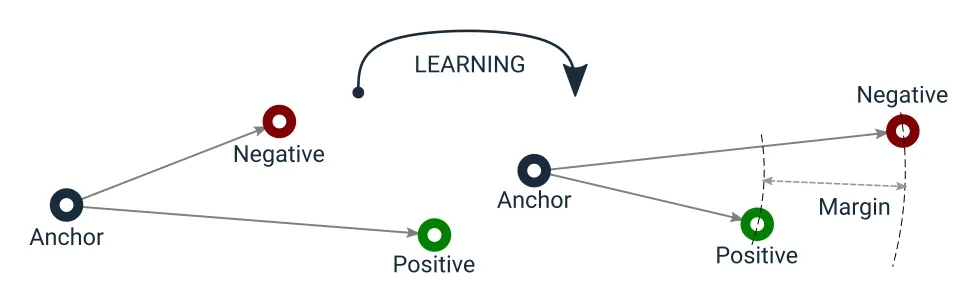
\includegraphics[scale=0.5]{chapters/nonstandart_error/images/triplet_loss_learning.png}
\end{figure}

\subsubsection*{Алгоритм формирования троек:}

обучение с триплет лоссом сильно зависит от алгоритма формирования троек.
Если формировать тройки случайно, то большинство троек будут слишком легкими, не информативными.
Негативные объекты будет слишком легко отличить от позитивных, поэтому обучающего сигнала от таких троек будет мало.
Поэтому хочется собрать наиболее сложные тройки из всех объектов в датасете или минибатче.
Такой процесс называется hard negative/positive mining и часто используется для обучения с триплетной функцией потерь.

\subsubsection*{Пример - задача поиска близких предложений}
\begin{itemize}
    \item в качестве позитивных объектов берем якорное предложение с опечатками, якорное предложение на других языках, с uppercase, lowercase буквами вперемешку
    \item в качестве негативных - другие предложения
\end{itemize}

\subsubsection*{Задача 1.}

Придумайте алгоритм подбора троек для задачи распознавания лиц

Ответ: 
\begin{itemize}
    \item в качестве позитивных объектов берем якорое лицо в другом освещение, с разных сторон
    \item в качестве негативных - лица другиз людей
\end{itemize}

\subsubsection*{Задача 2.}

Подумайте на что влияет $\alpha$, как будут меняться поведение модели при большом/нулевом $\alpha$

Ответ: роль $\alpha$ - значимое разделение классов, 
при нуле - не будет заметна разница между похожими и отличающимися объектами,
при слишком большом $\alpha$ - будем часто считать объекты одного класса различными

\subsubsection*{Задача 3.}

Реализуйте triplet loss с помощью PyTorch, для разных норм, сравните, есть ли отличия.


    \clearpage
    \chapter{Критерии выбора моделей}
    \section*{Качество классификации: Precision, Recall}

В задаче классификации \textbf{precision} (точность) и \textbf{recall} (полнота) являются ключевыми метриками для оценки качества предсказания, особенно в задачах с несбалансированными классами.

\subsection*{Определения}

Рассмотрим бинарную классификацию, то есть объект может быть либо положительным (positive), либо отрицательным (negative), и определим:

\begin{itemize}
    \item $TP$ (\textit{True Positives}) — количество объектов, правильно классифицированных как положительные.
    \item $FP$ (\textit{False Positives}) — количество объектов, ошибочно классифицированных как положительные.
    \item $FN$ (\textit{False Negatives}) — количество объектов, ошибочно классифицированных как отрицательные.
    \item $TN$ (\textit{True Negatives}) — количество объектов, правильно классифицированных как отрицательные.
\end{itemize}

На основе этих величин вычисляются:

\begin{enumerate}
    \item \textbf{Precision:}
    \[
    \text{Precision} = \frac{TP}{TP + FP}.
    \]
    Precision показывает долю истинно положительных объектов среди всех объектов, классифицированных как положительные.

    \item \textbf{Recall:}
    \[
    \text{Recall} = \frac{TP}{TP + FN}.
    \]
    Recall показывает долю истинно положительных объектов среди всех реально положительных объектов.
\end{enumerate}

\begin{figure}[ht!]
	\centering
	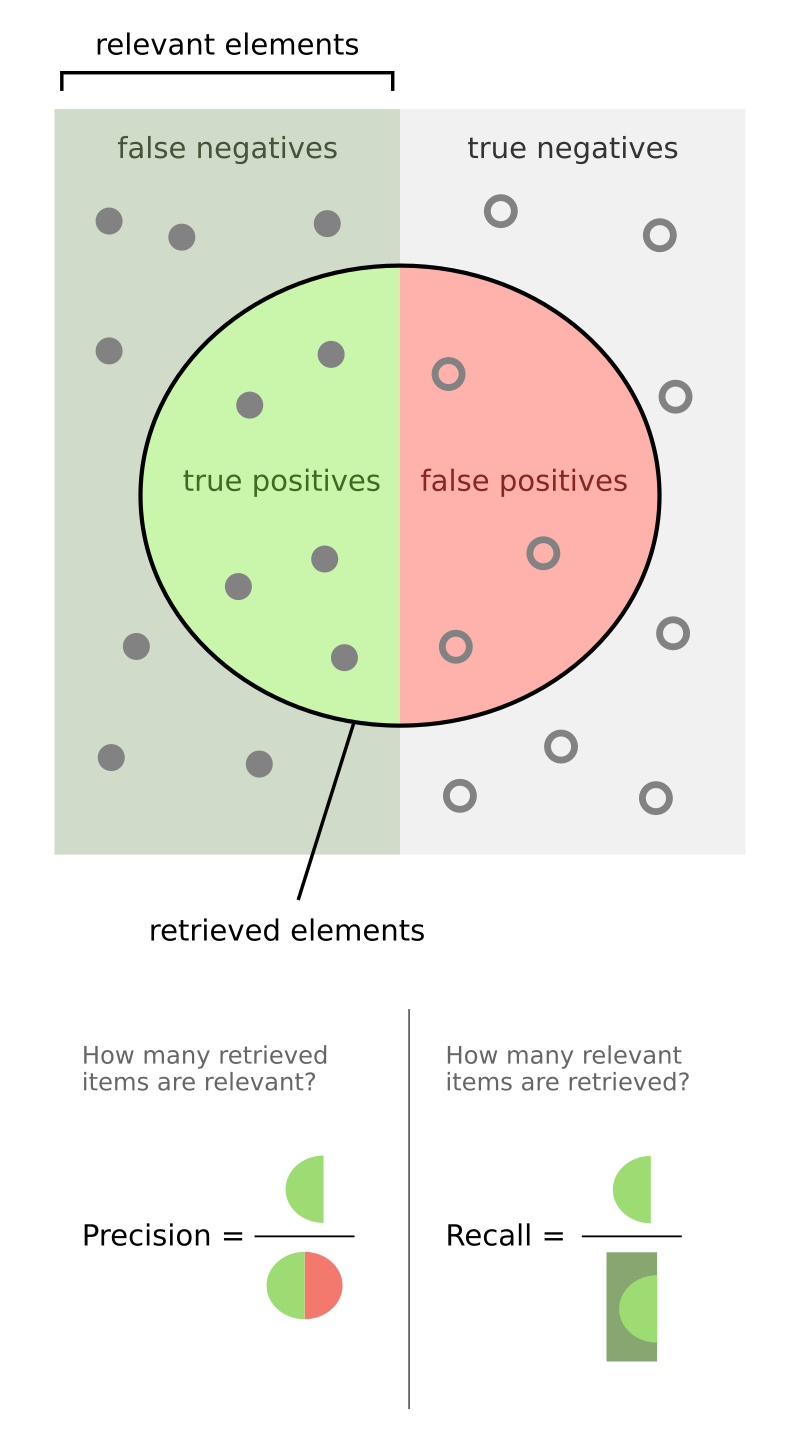
\includegraphics[width=0.65\linewidth]{chapters/model_selection/images/Precisionrecall.png}
\end{figure}

\subsection*{Интуитивное объяснение}

\begin{itemize}
    \item \textbf{Precision}: Насколько «точен» алгоритм, когда он говорит, что объект положительный? Если precision высокое, значит, ложные срабатывания ($FP$) минимальны.
    \item \textbf{Recall}: Насколько хорошо алгоритм находит все положительные объекты? Если recall высокое, значит, пропущенные положительные объекты ($FN$) минимальны.
\end{itemize}

\subsection*{Пример}

Классический пример использования метрик precision и recall - задача поиска спама на почте. В этом случае спам - положительная категория. Пусть у нас есть 100 писем, из которых 40 писем — спам, 60 писем — не спам.

Алгоритм классифицировал 50 писем как спам, из которых 30 писем действительно оказались спамом, а остальные 20 писем были ошибочно классифицированы как спам. Вычислим в этом случае precision и recall:

\begin{itemize}
    \item \textbf{Precision:}
    \[
    \text{Precision} = \frac{TP}{TP + FP} = \frac{30}{30 + 20} = 0.6.
    \]

    \item \textbf{Recall:}
    \[
    \text{Recall} = \frac{TP}{TP + FN} = \frac{30}{30 + 10} = 0.75.
    \]
\end{itemize}

\subsection*{Баланс между precision и recall}

Модель для каждого объекта на входе генерирует какое-то число на выходе. В простейшем варианте объект классифицируется как положительный, если это число больше некого выставленного порога, и как отрицательный в обратном случае. Увеличивая порог классификации, мы снижает количество False Positive объектов, потому precision увеличивается. При этом количество "незамеченных" моделью положительных объектов тоже вырастет, поэтому recall снизится. При уменьшении порога будет наблюдаться обратный эффект. Обычно стараются добиться компромиссного значения, при котором precision и recall оба принимают удовлетворительные значения. В некоторых случаях одна из метрик важнее другой:

\begin{itemize}
    \item Детекция спам-рассылок. В этом случае мы чаще всего не хотим пометить важные письма, как спам. Поэтому нужно снизить False Positive - важнее precision.
    \item Первичного выявление заболевания. Мы не хотим пропустить пациентов, которые на самом деле больны, только потому что модель сказала обратное. Поэтому важно снизить False Negative - в этом случае важнее recall. 
\end{itemize}

\subsection*{Интуитивное объяснение}

Если при получении положительного ответа от модели мы предпринимаем какое-либо действие, то precision важнее, когда действие обходится дорого, а recall важнее, когда бездействие обходится дорого. В примерах выше: помещение важного письма в папку "спам" (действие) может привести к финансовым потерям, а пропуск реального спама во "входящие" (бездействие) лишь заставит человека сделать это вручную. С другой стороны, при ложноположительном диагнозе человек пройдёт дополнительные анализы (действие), а ложноотрицательный может стоить ему жизни (бездействие).

\begin{figure}[ht!]
	\centering
	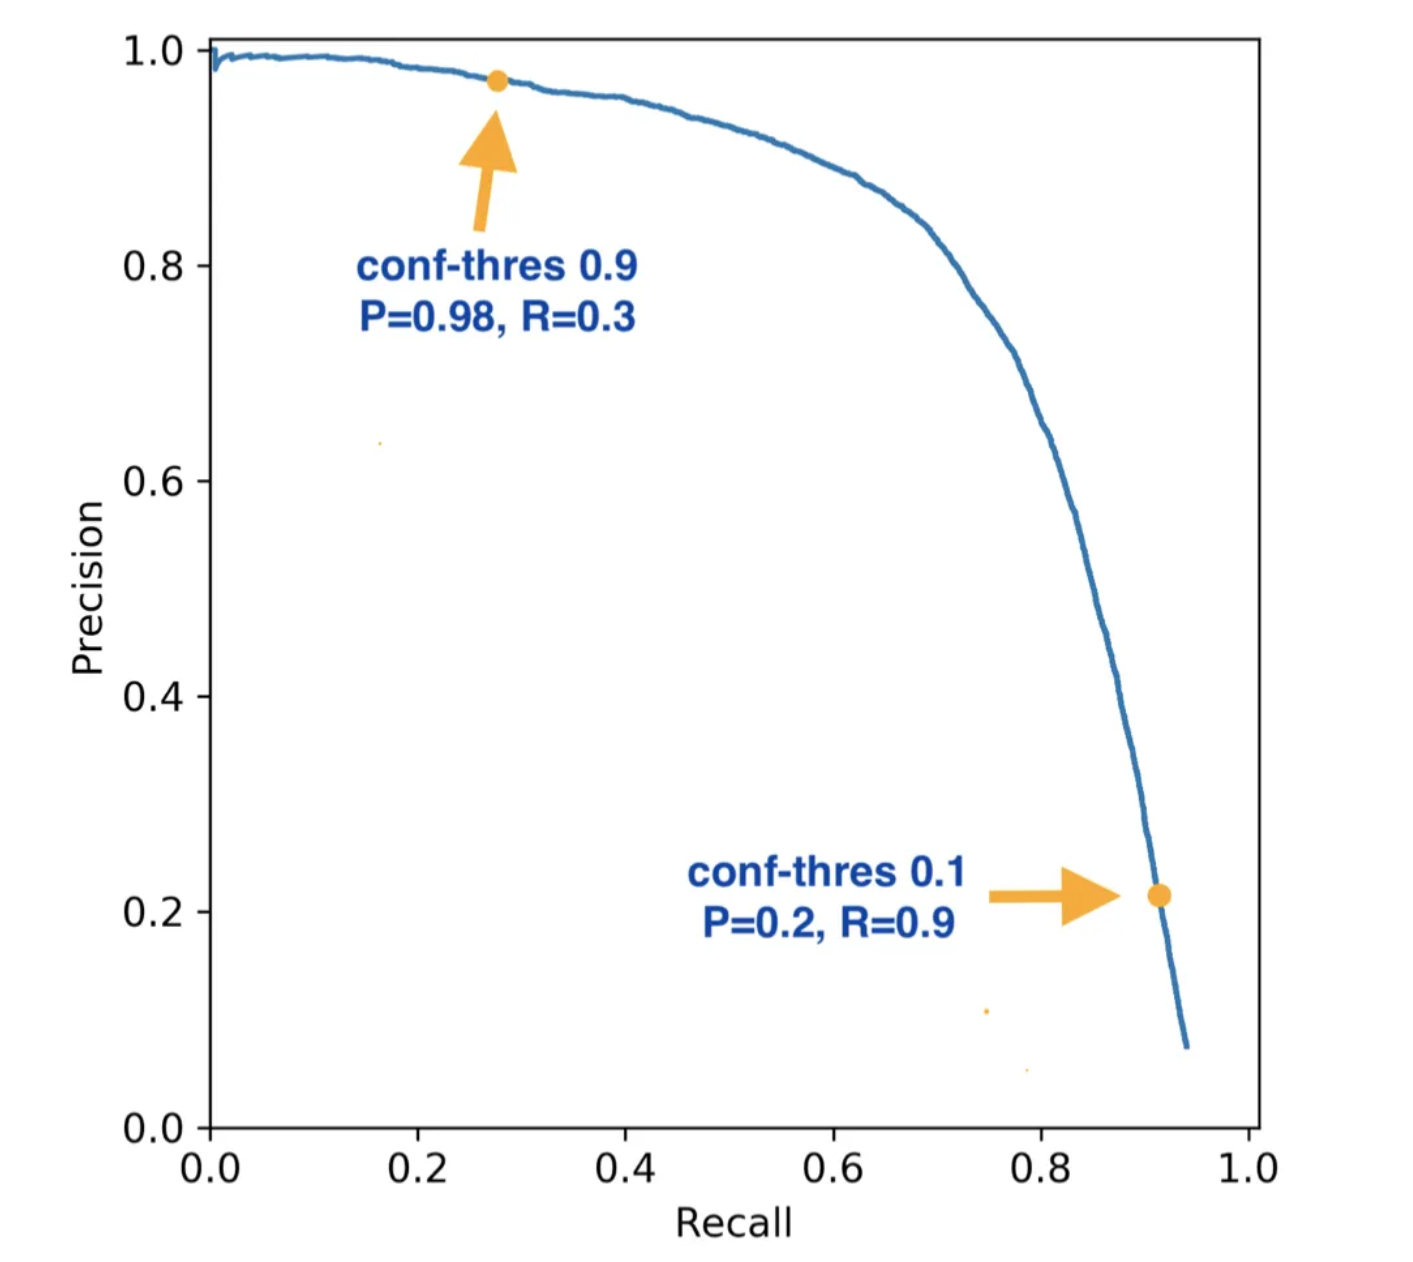
\includegraphics[width=0.65\linewidth]{chapters/model_selection/images/Precisionrecallcurve.png}
\end{figure}

\bigskip
\bigskip

Для того, чтобы изобразить баланс между двумя метриками, строят precision-recall кривую. Точки на ней соответствуют разным значениям порога.

\subsection*{F-метрика (дополнительно)}

Часто для оценки общего качества модели используется метрика $F$-мера, которая является гармоническим средним между precision и recall с параметром $\beta$:
\[
F_{\beta} = (1 + \beta^2) \cdot \frac{\text{Precision} \cdot \text{Recall}}{\beta^2 \cdot \text{Precision} + \text{Recall}}.
\]
Из формулы понятно, что $\beta$ определяет, насколько recall важнее по сравнению с precision. Наиболее часто используется $F_1$-мера:
\[
F_1 = 2 \cdot \frac{\text{Precision} \cdot \text{Recall}}{\text{Precision} + \text{Recall}}.
\]

\subsection*{Задачи}

\subsection*{Задача 1: Простейшая модель}

Как будет выглядеть precision-recall кривая у простейшей модели, которая для любого объекта делает positive предсказание с вероятностью $1-t$ (при $t = 1$ все предсказания отрицательные, при $t = 0.5$ - половина)? Как в этом случае и с использованием метрик precision и recall подбирать параметр $t$, чтобы добиться лучшей работы модели?

\textbf{Ответ:}

В координатах ($recall$, $precision$) - отрезок с концами в (0, $\alpha$) и (1, $\alpha$), где $\alpha$ - доля положительных объектов в выборке (горизонтальный отрезок). Объяснение состоит в том, что доля $TP$ равна $\alpha (1-t)$, доля $TP + FN$ равна $\alpha$, а доля $TP + FP$ равна $(1-t)$. Таким образом, значения precision и recall не зависят от параметра $t$, то есть его изменение не изменит качество модели в этих метриках.

\subsection*{Задача 2: Дисбаланс классов}

Какая из метрик -- precision или recall -- будет больше в случае сильного дисбаланса классов на тестовой выборке (рассмотреть оба случая), если известно, что модель обучалась на сбалансированном датасете?

\textbf{Ответ:}

Если положительных объектов значительно меньше, чем отрицательных, то recall будет больше. Это связано с тем, что сбалансированная модель в этом случае будет допускать много False Positive ошибок. При обратном дисбалансе precision будет больше из-за большого количества False Negative ошибок.

\subsection*{Задача 3: Мошеннические транзакции}

Финансовая компания использует алгоритм для выявления мошеннических транзакций. Из 10,000 проверенных транзакций 500 транзакций являются мошенническими, 9,500 транзакций являются легитимными.

Алгоритм определил 600 транзакций как мошеннические, из которых 400 действительно оказались мошенническими.

\begin{enumerate}
    \item Вычислите $F_1$-меру.
    \item Насколько может измениться $F_1$-мера, если алгоритм пометит ещё 50 транзакций как мошеннические, в зависимости от того, являются они на самом деле мошенническими или нет?
\end{enumerate}

\textbf{Решение:}
Найдём precision и recall.
\begin{itemize}
    \item
    \[
    \text{$precision$} = \frac{400}{400 + 200} = \frac{400}{600} \approx 0.667.
    \]
    \item
    \[
    \text{$recall$} = \frac{400}{400 + 100} = \frac{400}{500} = 0.8.
    \]
    \item
    \[
    \text{$F_1$-score} = 2\frac{precision\cdot recall}{precision + recall} = 2\frac{0.667\cdot 0.8}{0.667 + 0.8} \approx 0.722
    \]

\end{itemize}

Обозначим за $\alpha$ долю тех новых помеченных транзакций, которые на самом деле являются мошенническими ($0 \le \alpha \le 1$). Понятно, что $TP$ увеличится на $50\alpha$, $FN$ уменьшится на $50\alpha$, а $TP + FP$ станет равным 650. Посчитаем precision, recall, изменение $F_1$-score в общем случае:

\begin{itemize}
    \item
    \[
    \text{$precision$} = \frac{400 + 50\alpha}{650}.
    \]
    \item
    \[
    \text{$recall$} = \frac{400 + 50\alpha}{500}.
    \]
    \item
    \[
    \text{$F_1$-score} = \frac{16 + 2\alpha}{23} \approx 0.696 + 0.087\alpha
    \]
    \item
    \[
    \text{$\Delta F_1$-score} \approx 0.696 + 0.087\alpha - 0.722 = -0.026 + 0.087\alpha
    \]
\end{itemize}

Таким образом, $F_1$-мера уменьшится на -0.026 если все новые помеченные транзакции на самом деле легитимные, увеличится на 0.061, если они все на самом деле мошеннические. Заметим, что $F_1$-мера останется неизменной, если $\alpha = \frac{1}{3}$, то есть изначальная доля ложноположительных среди всех помеченных.


\section*{Аналитические внутренние критерии}

При выборе модели машинного обучения
\[
f : \mathbb{X} \to \mathbb{Y},
\]
модель выбирается согласно некоторого критерия $L$ (функции ошибки, минус логарифм правдоподобия и т.д.). Обычно в качестве функции $L$ рассматривается некоторая функция ошибки модели $f$ на выборке $\mathcal{D}$:
\[
f = \underset{f \in \mathfrak{F}}{\arg\min} \ L(f, \mathcal{D}).
\]

В зависимости от вида функции $L$ разделяют два типа критериев:
\begin{enumerate}
    \item внутренний критерий качества;
    \item внешний критерий качества.
\end{enumerate}

\subsection*{Типы выборок}
Далее будем рассматривать два типа выборок:
\begin{enumerate}
    \item $\mathcal{D}$ --- это вся выборка, которая доступна для выбора модели;
    \item $\mathcal{D}'$ --- это выборка, на которой проверяется качество уже выбранной модели;
    \item $\mathcal{D}^l_k$ --- это $k$-я подвыборка выборки $\mathcal{D}$ размера $l_k$.
\end{enumerate}

\subsection*{Внутренние и внешние критерии}
\textbf{Внутренний критерий качества} используется для оценки модели на той же выборке, на которой она обучалась. Примером внутреннего критерия является:
\[
Q_{\text{внутренний}}(w, \mathcal{D}) = \frac{1}{|\mathcal{D}|} \sum_{i=1}^{|\mathcal{D}|} L(f(x_i, w), y_i),
\]
где $L$ --- функция ошибки, $w$ --- параметры модели, $(x_i, y_i)$ --- объекты выборки $\mathcal{D}$. 

\textbf{Внешний критерий качества} оценивает качество модели на независимой выборке $\mathcal{D}'$, не использовавшейся при обучении. Примером внешнего критерия является:
\[
Q_{\text{внешний}}(w, \mathcal{D}') = \frac{1}{|\mathcal{D}'|} \sum_{i=1}^{|\mathcal{D}'|} L(f(x_i, w), y_i).
\]

\subsection*{Регуляризация и внутренние критерии}
Регуляризованный внутренний критерий используется для выбора оптимальной модели с учётом её сложности:
\[
Q_{\text{рег}}(w, \mathcal{D}) = Q(w, \mathcal{D}) + \tau R(w),
\]
где $R(w)$ --- регуляризатор, штрафующий за сложность модели, а $\tau$ --- коэффициент регуляризации.

\subsection*{VC-оценка}
Для оценки обобщающей способности модели используется VC-оценка, основанная на VC-размерности модели $h$:
\[
VC(w, \mathcal{D}) = Q_{\text{внутренний}}(w, \mathcal{D}) + \sqrt{\frac{h}{|\mathcal{D}|} \ln \frac{2e|\mathcal{D}|}{h}}.
\]

\subsection*{Сложность модели и переобучение}
Сложность модели напрямую влияет на внутренние и внешние критерии:
\begin{itemize}
    \item При увеличении сложности модели внутренний критерий качества уменьшается, так как модель лучше подстраивается под обучающие данные.
    \item Однако внешний критерий качества может начать ухудшаться из-за переобучения, когда модель теряет обобщающую способность.
\end{itemize}

\subsection*{Задача 1: Влияние сложности модели на внутренний критерий}

Положим, что внутренний критерий модели монотонно уменьшается с увеличением числа признаков $n$, тогда как внешний критерий имеет минимум при $n = 5$. На выборке из $\ell = 150$ объектов модель с 3 признаками имеет $Q_{\text{внутренний}} = 0.08$, а модель с 6 признаками имеет $Q_{\text{внутренний}} = 0.05$. 

\begin{enumerate}
    \item Почему использование внутреннего критерия для выбора $n$ может привести к ошибке?
    \item Какой подход лучше использовать в данном случае для выбора оптимального $n$?
\end{enumerate}

\subsection*{Решение:}

\begin{enumerate}
    \item Внутренний критерий убывает с увеличением сложности модели, что может привести к выбору слишком сложной модели, склонной к переобучению. Он не учитывает обобщающую способность модели.
    \item Лучше использовать внешний критерий, например, кросс-валидацию или разбиение на обучающую и тестовую выборки, так как они учитывают качество модели на независимых данных.
\end{enumerate}


\subsection*{Задача 2: Применение VC-оценки}

Пусть для линейной классификации на выборке из $\ell = 200$ объектов используется модель с VC-размерностью $h = 10$. Обучающая ошибка модели равна $Q_{\text{внутренний}}(w, X^\ell) = 0.05$. Используя упрощённую формулу VC-оценки:
\[
VC(w, X^\ell) = Q_{\text{внутренний}}(w, X^\ell) + \sqrt{\frac{h}{\ell} \ln \frac{2e\ell}{h}},
\]
рассчитайте VC-критерий.

\subsection*{Решение:}

Подставляем значения:
\[
VC(w, X^\ell) = 0.05 + \sqrt{\frac{10}{200} \ln \frac{2e \cdot 200}{10}}.
\]

Вычислим:
\[
\frac{10}{200} = 0.05, \quad \ln \frac{2e \cdot 200}{10} = \ln 40e \approx \ln 40 + 1 \approx 3.69.
\]
\[
VC(w, X^\ell) = 0.05 + \sqrt{0.05 \cdot 3.69} \approx 0.05 + \sqrt{0.1845} \approx 0.05 + 0.43 = 0.48.
\]


\subsection*{Задача 3: Оценка с использованием аналитического внутреннего критерия}

У вас есть модель линейной регрессии, обученная на выборке размером $\ell = 100$. Функционал качества модели $Q(w, X^\ell)$ на обучающей выборке составляет $0.02$, а регуляризатор $R(w)$ для модели рассчитывается как 
\[
R(w) = \tau \|w\|^2,
\]
где $\|w\|^2 = 1.5$, а $\tau = 0.1$. 

\begin{enumerate}
    \item Вычислите регуляризованный критерий качества модели $Q_{\text{рег}}(w, X^\ell)$.
    \item Объясните, как изменение значения $\tau$ влияет на выбор модели.
\end{enumerate}

\subsection*{Решение:}

\begin{enumerate}
    \item
    \[
    Q_{\text{рег}}(w, X^\ell) = Q(w, X^\ell) + \tau \|w\|^2 = 0.02 + 0.1 \cdot 1.5 = 0.17.
    \]
    \item Увеличение $\tau$ повышает штраф за сложность модели, что приводит к предпочтению более простых моделей. При уменьшении $\tau$ модель становится менее регуляризованной, что повышает риск переобучения.
\end{enumerate}

\section{Применение обоснованности при выборе модели}

\subsection{Мотивация введения понятия обоснованности}

В процессе анализа данных и построения моделей мы сталкиваемся с необходимостью выбора наилучшей модели среди множества возможных вариантов. Однако традиционные подходы, такие как минимизация ошибки на обучающей выборке, могут привести к переобучению и, следовательно, плохой обобщаемости модели на новых данных. Чтобы избежать этого, необходимо оценивать качество модели не только по ее способности предсказывать известные данные, но и по тому, насколько она совместима с предполагаемым распределением данных.

Именно здесь возникает понятие обоснованности, которое помогает нам сравнивать разные модели на основе вероятности того, что они могли бы породить наблюдаемые данные. В отличие от других критериев, таких как точность на тестовой выборке или ошибка обучения, обоснованность учитывает как сложность модели, так и ее способность объяснять данные без чрезмерного усложнения.

\subsection{Определение обоснованности}

Обоснованность (или marginal likelihood) — это вероятность наблюдаемых данных при условии выбранной модели. Она выражается следующим образом:

\begin{equation}
    p(\mathbf{X} \mid \mathcal{M}) = \int p(\mathbf{X} \mid \boldsymbol{\theta}, \mathcal{M}) \, p(\boldsymbol{\theta} \mid \mathcal{M}) \, d\boldsymbol{\theta}
\end{equation}

Где:$\mathbf{X}$ — наблюдаемая выборка данных,$\mathcal{M}$ — рассматриваемая модель, $\boldsymbol{\theta}$ — вектор параметров модели, $p(\mathbf{X} \mid \boldsymbol{\theta}, \mathcal{M})$ — функция правдоподобия данных при фиксированных значениях параметров, $p(\boldsymbol{\theta} \mid \mathcal{M})$ — априорное распределение параметров модели.

Интеграция по параметрам $\boldsymbol{\theta}$ означает усреднение правдоподобия по всем возможным значениям параметров, взвешенным согласно их априорной вероятности. Таким образом, обоснованность показывает, насколько хорошо модель объясняет данные, учитывая все возможные комбинации значений параметров.

\subsubsection{Задача 1: Обоснованность для модели линейной регрессии}
Пусть имеется модель линейной регрессии с нормальным шумом
\begin{equation*}
 \mathbf{y} = \mathbf{X}\mathbf{w} + \boldsymbol{\varepsilon}, \quad \boldsymbol{\varepsilon} \sim \mathcal{N}(0, \sigma^2 \mathbf{I}),
\end{equation*}
где $\sigma^2$ --- известно, и априорным распределением на $\mathbf{w}$ $p(\mathbf{w}) = \mathcal{N}(\mathbf{w} \mid \mathbf{m}, \alpha^2 \mathbf{I}))$, где $\mathbf{m}$ и $\alpha$ ---
неизвестные гиперпараметры.

Найдите обоснованность модели $p(\mathbf{y} \mid \mathbf{X}, \mathbf{m}, \alpha)$ с точностью до константы.

\subsubsection*{Решение}

Функция правдоподобия для нашей модели линейной регрессии с нормальными ошибками записывается как:

\begin{align*}
 p(\mathbf{y} \mid \mathbf{X}, \mathbf{w}, \sigma^2) &= \mathcal{N}(\mathbf{y} \mid \mathbf{X}\mathbf{w}, \sigma^2 \mathbf{I}) \\
 &\propto \exp\left(-\frac{1}{2\sigma^2}(\mathbf{y} - \mathbf{X}\mathbf{w})^\top(\mathbf{y} - \mathbf{X}\mathbf{w})\right)
\end{align*}

где $N$ — число наблюдений, а $\mathbf{I}$ — единичная матрица размера $N \times N$.

Априорное распределение для $\mathbf{w}$:

\begin{align*}
 p(\mathbf{w} \mid \mathbf{m}, \alpha^2) &= \mathcal{N}(\mathbf{w} \mid \mathbf{m}, \alpha^2 \mathbf{I}) \\
 &\propto \exp\left(-\frac{1}{2\alpha^2}(\mathbf{w} - \mathbf{m})^\top(\mathbf{w} - \mathbf{m})\right)
\end{align*}

где $d$ — размерность вектора $\mathbf{w}$.

Маргинальная вероятность (обоснованность) находится путём интегрирования произведения правдоподобия и априорного распределения по $\mathbf{w}$:

\begin{align*}
 p(\mathbf{y} \mid \mathbf{X}, \mathbf{m}, \alpha) &= \int p(\mathbf{y} \mid \mathbf{X}, \mathbf{w}, \sigma^2) p(\mathbf{w} \mid \mathbf{m}, \alpha^2) \, d\mathbf{w} \propto \\
 &\propto \int \exp\left(-\frac{1}{2\sigma^2}(\mathbf{y} - \mathbf{X}\mathbf{w})^\top(\mathbf{y} - \mathbf{X}\mathbf{w}) - \frac{1}{2\alpha^2}(\mathbf{w} - \mathbf{m})^\top(\mathbf{w} - \mathbf{m})\right) \, d\mathbf{w}.
\end{align*}

Приведём выражение внутри экспоненты к квадратичной форме:

\begin{align*}
 &-\frac{1}{2\sigma^2}(\mathbf{y} - \mathbf{X}\mathbf{w})^\top(\mathbf{y} - \mathbf{X}\mathbf{w}) - \frac{1}{2\alpha^2}(\mathbf{w} - \mathbf{m})^\top(\mathbf{w} - \mathbf{m})= \\
 &= -\frac{1}{2}(\mathbf{w} - \mathbf{b})^\top A^{-1} (\mathbf{w} - \mathbf{b}) + \frac{1}{2} b^\top A^{-1} b + \text{const},
\end{align*}

где $\mathbf{A}$ и $\mathbf{b}$ равны следующим выражениям:
\begin{align*}
 A &= \left(\frac{\mathbf{X}^\top \mathbf{X}}{\sigma^2} + \frac{\mathbf{I}}{\alpha^2}\right)^{-1},\\
 \mathbf{b} &= \frac{1}{\sigma^2} \mathbf{X}^\top \mathbf{y} + \frac{1}{\alpha^2} \mathbf{m}.
\end{align*}

Подставим в интеграл полученное выражение:
\begin{align*}
 p(\mathbf{y} \mid \mathbf{X}, \mathbf{m}, \alpha) &\propto \int \exp\left(-\frac{1}{2}(\mathbf{w} - \mathbf{b})^\top \mathbf{A}^{-1} (\mathbf{w} - \mathbf{b}) + \frac{1}{2} \mathbf{b}^\top \mathbf{A}^{-1} \mathbf{b} \right) \, d\mathbf{w}.
\end{align*}
Этот интеграл пропорционален $\propto\exp\left(\dfrac{1}{2} \mathbf{b}^\top \mathbf{A}^{-1} \mathbf{b}\right) \sqrt{\det \mathbf{A}}$, поскольку интеграл экспоненты от полного квадрата пропорционален $\sqrt{\det \mathbf{A}}$.

\textbf{Ответ:} $p(\mathbf{y} \mid \mathbf{X}, \mathbf{m}, \alpha) \propto\exp\left(\dfrac{1}{2} \mathbf{b}^\top \mathbf{A}^{-1} \mathbf{b}\right) \sqrt{\det \mathbf{A}}$, где
\begin{align*}
 \mathbf{A} &= \left(\frac{\mathbf{X}^\top \mathbf{X}}{\sigma^2} + \frac{\mathbf{I}}{\alpha^2}\right)^{-1},\\
 \mathbf{b} &= \frac{1}{\sigma^2} \mathbf{X}^\top \mathbf{y} + \frac{1}{\alpha^2} \mathbf{m}.
\end{align*}

\subsubsection{Задача 2: Применение обосонованности при выборе модели}
Подумайте, как можно выбирать модели в задачах классификации и регресии, используя обоснованность.
\subsubsection{Решение}

Интуитивная интерпретация обоснованности говорит, что чем она больше, тем лучше модель описывает данные из выборки. Поэтому хочется построить следующий принцип: всегда выбирать наиболее подходящую с точки зрения обоснованности модель. Этот метод имеет место на жизнь и в задаче регресии, и в задаче классификации.

Другой метод, которых приходит на ум --- это взвешенное голосование моделей с весами, пропорциональными обоснованности. Он также хорошо подойдет, поскольку модели, плохо описывающие данную выборку получат маленькие веса, а хорошо описывающие, напротив --- большие. И тогда в среднем мы получим хороший прогноз. Этот метод тоже подходит и для задачи классификации, и для задачи регресии.

\subsubsection{Задача 3: Недостатки обоснованности}
Как вы думаете, какие недостатки применения обоснованности на практике?
\subsubsection{Решение}

Их можно выделить несколько:
\begin{itemize}
 \item Сложность вычисления интеграла по всем возможным параметрам $\theta$. Если представить, что мы хотим применить наш подход, например, в глубоких нейронных сетях на миллионы параметров, то взять интеграл из определения обоснованности попросту невозможно. Более того, не всегда он будет браться аналитически, и тогда придется либо нижние оценки, либо считать его сэмплированием, из-за чего пострадает качество и что тоже достаточно сложно или дорого вычислительно.
 \item Мы не всегда знаем, из каких априорных распределений берутся параметры модели. В простых задачах, по типу линейной или логистической регресии, мы можем наложить нормальное априорное распределение и получить неплохую модель. Но например в тех же глубоких нейронных сетях или более сложных моделях, может быть такое, что мы даже предположить не можем, какое априорное распределение взять.
\end{itemize}


\section*{Аналитические внешние критерии}

\par Аналитические внешние критерии используются для отслеживания сложности используемой модели. Это необходимо для того, чтобы находить баланс между точностью модели на обучающей выборке и её обобщающей способностью.

\subsection*{Критерии регуляризации}

\par \textbf{Регуляризатор} - аддитивная добавка к внутреннему критерию, обычно штраф за сложность (complexity penalty) модели $A$. 

\begin{align*}
    Q_{per} (\mu, X^l) = Q_{\mu}(X^l) + \text{штраф}(A)
\end{align*}


\par Для линейных моделей

1. Классификация $A = \{a(x) = \text{sign}\langle w, x \rangle\}$

2. Регрессия $A = \{a(x) = \langle w, x \rangle \}$

\par Существуют следующие виды регуляризации

\begin{enumerate}
    \item $L_2$-регуляризация (RIDGE)
        \begin{align*}
            \text{штраф}(A) =  \tau \|w\|_2^2 = \tau \sum\limits_{i = 1}^n w_i^2
        \end{align*}
        Может приводить к обнулению некоторых, несущественных признаков, что делает модель более разреженной
    \item $L_1$-регуляризация (LASSO)
        \begin{align*}
            \text{штраф}(A) = \tau \|w\|_1 = \tau \sum\limits_{i = 1}^n |w_i|
        \end{align*}
    \item $L_0$-регуляризация (AIC, BIC):
        \begin{align*}
            \text{штраф}(A) = \tau\|w\|_0 = \tau\sum\limits_{i = 1}^n [w_i \neq 0]
        \end{align*}
        т.е. штрафует за количество используемых параметров
\end{enumerate}

\subsection*{Разновидности $L_0$ регуляризации}

\begin{enumerate}
    \item Информационный критерий Акаике 
        \begin{align*}
            \text{AIC}(\mu, X^l) = Q_{\mu}(X^l) + \frac{2\hat{\sigma}^2}{l}|J|
        \end{align*}
        где $J$ - модмножество используемых параметров, а $\hat{\sigma}^2$ - оценка дисперсии ошибки $\mathbb{D}[y_i - a(x_i)]$ 
    \item Байесовский информационный критерий
        \begin{align*}
            \text{BIC}(\mu, X^l) = \frac{l}{\hat{\sigma}^2}\left(Q_{\mu}(X^l) + \frac{\hat{\sigma}^2\ln{l}}{l}|J|\right)
        \end{align*}
    \item Оценка Вапника-Червоненкиса (VC-bound)
        \begin{align*}
            VC(\mu, X^l) = Q_{\mu}(X^l) + \sqrt{\frac{h}{l}\ln{\frac{2el}{h}} + \frac{1}{l}\ln{\frac{9}{4\eta}}}
        \end{align*}
        где $h$ - VC-размерность, которая для линейных моделей равна $|J|$, $\eta$ - уровень значимости, обычно равный $0.05$
\end{enumerate}

\subsection*{Задачи}

\begin{enumerate}
    \item \textbf{Задача 1}
    
        Рассмотрим задачу линейной регрессии, вектор весов $w= [2, -1, 0, 3]$. Тренировочные данные:
        \begin{align*}
            X = \begin{bmatrix}
            1 & 2 & 3 & 4 \\
            2 & 0 & 1 & 3 \\
            3 & 1 & 0 & 2 
            \end{bmatrix} 
        \end{align*}
        \begin{align*}
            y = [10,8,7]
        \end{align*}
        Найдите:
        \begin{itemize}
        \item L2, L1, L0 штрафы
        \item BIC и AIC
        \end{itemize}
        $\tau$ везде принять за 1
        
        \textbf{Решение:} Не выписывая все выкладки, выпишем ответы:
        \begin{itemize}
            \item $L1 = \|w\|_1 = 6$
            \item $L2 = \|w\|_2^2 = 14$
            \item $L0 = \|w\|_0 = 3$
        \end{itemize}
        Для поиска AIC и BIC поднадобится дисперсия
        \begin{align*}
            \hat{\sigma}^2 = 15.0
        \end{align*}
        Тогда
        \begin{itemize}
            \item AIC = 14.12
            \item BIC = 11.42
        \end{itemize}
    \item \textbf{Задача 2}

        Докажите, что увеличение объёма выборки $l$ снижает влияние VC-размерности на обобщающую ошибку, если уровень значимости $\eta$ остаётся неизменным. Какой у этого физический смысл?

        \textbf{Решение: }
            VC-bound можно переписать следующим образом
            \begin{align*}
                VC(\mu, X^l) = Q_{\mu}(X^l) + \sqrt{\frac{h\ln{l\frac{2e}{h}} + \ln{\frac{9}{4\eta}}}{l}}
            \end{align*}
            То есть $VC(\mu, X^l) \sim Q_{\mu}(X^l) + \sqrt{\frac{\ln{l}}{l}}$
            Второ слагаемое стремится к нулю при $l \rightarrow \inf$. Это означает, что модель достаточно устойчива к переобучению при большой тренировочной выборке, поэтому внешний штраф не так уж и нужен и большую роль влияет внутренний критерий.
    \item \textbf{Задача 3}

        Объясните, почему L2-регуляризация не приводит к разреженности вектора параметров $w$, в отличие от L1-регуляризации.
\end{enumerate}

    \clearpage
    \chapter{Методы отбора признаков}
    \section{Методы отбора признаков}


\subsection*{Постановка задачи}
Пусть исходный набор признаков состоит из \( n \) элементов. Тогда задача отбора признаков формализуется следующим образом: 
Найти подмножество $S \subseteq \{1, 2, \dots, n\}$, такое, что $f(S)$ максимизирует (или минимизирует) целевую функцию. Где \( $f(S)$ \) — метрика, характеризующая качество модели (например, точность, $ R^2 $, AUC-ROC).

Сложность задачи заключается в её комбинаторной природе: общее количество подмножеств \( S \) равно \( 2^n \). Для больших \( n \) полный перебор становится вычислительно неэффективным.

\subsection*{Классификация алгоритмов}

\textbf{1. Фильтрационные методы}
Фильтрационные методы работают независимо от модели и используют статистические меры для оценки значимости признаков.

Примеры:
\begin{itemize}
    \item Многорядный итерационный алгоритм МГУА 
\end{itemize}

\textbf{2. Обёрточные методы}
Обёрточные методы оценивают подмножества признаков на основе качества модели, что обеспечивает высокую точность, но увеличивает вычислительную сложность.  

Примеры:
\begin{itemize}
    \item Полный перебор.
    \item Метод добавления и удаления (шаговая регрессия).
    \item Поиск в глубину.
    \item Метод ветвей и границ.
\end{itemize}

\textbf{3. Встроенные методы}
Встроенные методы выбирают признаки в процессе построения модели, используя регуляризацию или другие встроенные механизмы.  

Примеры:
\begin{itemize}
    \item L2, L1, L0-регуляризация 
\end{itemize}

\textbf{4. Эвристические и случайные методы}
Эти методы используют эвристики или случайный подход для нахождения подмножеств признаков, что снижает вычислительную сложность.  

Примеры:
\begin{itemize}
    \item Генетический алгоритм
    \item Случайный поиск 
    \item Случайный поиск с адаптацией (СПА) 
\end{itemize}

\subsection*{Задача 1: Выбор оптимального метода отбора признаков}

\textbf{Условие задачи}
Имеется набор данных, содержащий: 20 признаков \( X_1, X_2, \dots, X_{20} \), 500 записей, целевую переменную \( Y \). 
Цель — построить модель линейной регрессии, которая предсказывает \( Y \) с минимальной среднеквадратической ошибкой (MSE).  
\subsubsection*{Ограничения:}
\begin{enumerate}
    \item Требуется сократить число признаков, чтобы модель была проще и быстрее, но при этом сохранить качество.  
    \item Время на выполнение задачи ограничено: не более 5 минут вычислений.  
\end{enumerate}

\textbf{Вопрос:} Какой метод вы выберете для решения задачи? Обоснуйте выбор и оцените его время работы.
\subsection*{Задача 2: Полный перебор для отбора признаков}

\textbf{Условие задачи}
Дан набор данных с 4 признаками: $X_1, X_2, X_3, X_4$
Необходимо:  
\begin{enumerate}
    \item Перебрать все возможные подмножества признаков.
    \item Для каждого подмножества вычислить точность модели классификации.
    \item Найти подмножество, обеспечивающее максимальную точность.
\end{enumerate}

\textbf{Вопросы}
 Можно ли было применить более быстрый метод вместо полного перебора?

\subsection*{Задача 3}

Рассмотрите три задачи:  
\begin{enumerate}
    \item Для набора данных с 5 признаками требуется построить модель линейной регрессии с минимальной среднеквадратической ошибкой. Время на выполнение не ограничено.  
    \item Для набора данных с 50 признаками и 1000 объектов необходимо выбрать наиболее значимые признаки для задачи классификации. Требуется уложиться в 10 минут вычислений.  
    \item Для набора данных с 20 признаками известны сильные корреляции между некоторыми из них. Задача — исключить избыточные признаки и построить компактную модель.  
\end{enumerate}

Какой тип метода отбора признаков (\textbf{фильтрационный}, \textbf{обёрточный} или \textbf{встроенный}) вы бы выбрали для каждой задачи? Обоснуйте свой выбор.


\section{Качество классификации}
Рассмотрим задачу бинарной классификации с обучающей выборкой $D = \{(x_i, y_i)\}_{i=1}^n$, где $x_i \in \mathbb{R}^d$ --- вектор признаков, $y_i \in \{0, 1\}$ --- бинарная переменная.
Мы хотим построить модель $f: \mathbb{R}^d \to \{0, 1\}$, которая принимает на вход вектор признаков и выдает предсказание класса.
Есть следующие способы измерять качество модели:

Accuracy

Precision

Recall

$F_{\beta}$ score

ROC AUC

Для каждого объекта из выборки мы имеем 4 варианта разивития событий:

TP --- True Positive, классификатор предсказал 1, верное значение тоже 1

FP --- False Positive, классификатор предсказал 1, верное значение 0

TN --- True Negative, классификатор предсказал 0, верное значение тоже 0

FN --- False Negative, классификатор предсказал 0, верное значение 1


Ясно, что мы хотим видеть как можно больше TP и TN и как можно меньше FP и FN.

Accuracy --- это доля правильных ответов классификатора.
$$
    \text{Accuracy} = \frac{TP + TN}{TP + FP + TN + FN} = \frac{1}{n} \sum_{i=1}^n \mathbb{I}(y_i = f(x_i))
$$

Достаточно банальная метрика, которая не учитывает дисбаланса классов, но в качестве базового варианта подходит отлично.

Precision --- это доля объектов, которые классификатор предсказал как 1, среди всех объектов, которые он предсказал как 1.
$$
    \text{Precision} = \frac{TP}{TP + FP}
$$

Recall --- это доля объектов, которые классификатор предсказал как 1, среди всех объектов, которые действительно равны 1.
$$
    \text{Recall} = \frac{TP}{TP + FN}
$$

Precision и Recall --- базовые метрики, но по отдельности их использовать нельзя, поэтому придумали $F_{\beta}$ score.

$F_{\beta}$ score --- это взвешенное среднее гармоническое precision и recall.
$$
    F_{\beta} = (1 + \beta^2) \frac{precision \cdot recall}{\beta^2 \cdot precision + recall}
$$

$TPR$ --- это доля объектов, которые классификатор предсказал как 1, среди всех объектов, которые действительно равны 1.
$$
    TPR = \frac{TP}{TP + FN}
$$

$FPR$ --- это доля объектов, которые классификатор предсказал как 1, среди всех объектов, которые действительно равны 0.
$$
    FPR = \frac{FP}{FP + TN}
$$

Обычно, когда мы решаем задачу бинарной классификации, то мы не предсказываем явный класс, а предсказываем какое-то значение, и чем больше это значение, тем больше вероятность того, что объект принадлежит к классу 1.
Следовательно, мы можем устанавливать пороговое значение, которое будет определять, к какому классу отнести объект.
При увеличении порога отсечения мы увеличиваем количество объектов, которые отнесены к классу 0, и уменьшаем количество объектов, которые отнесены к классу 1.
Заметим, что также при увеличении порога отсечения TPR и FPR будут уменьшаться.

ROC кривая --- это кривая, которая показывает зависимость TPR от FPR при изменении порога отсечения. То есть по оси $x$ откладывается $FPR$, а по оси $y$ --- $TPR$.

Строго говоря, ROC кривая --- это множество точек вида $(FPR(t), TPR(t))$, где $t$ --- пороговое значение вероятности.

ROC-AUC --- это площадь под ROC кривой.

\subsection*{Задача 1}

Мы хотим построить модель бинарной классификации, которая будет по некоторому описанию пациента предсказывать, болен ли он раком.
В случае, если наша модель скажет, что пациент болен раком, то мы отправим его на дополнительное обследование, что обойдется пациенту в некоторую неприятную, но не критичную сумму денег.
Если же наша модель скажет, что пациент здоров, то мы ничего не будем предпринимать.
Мы хотим выбрать метрику качества для нашей модели из следующего списка: Accuracy, Precision, Recall, $F_{\beta}$ score, что нам лучше всего подойдет?
Если мы хотим выбрать $F_{\beta}$ score, то какие значения $\beta$ нам лучше всего подойдут?

\subsection*{Решение}
Accuracy --- не лучший вариант, так как ошибка FP и FN в нашем случае не равнозначны.
Не отправить больного на дополнительное обследование значительно хуже, чем отправить здорового пациента на обследование.
Precision и Recall --- достаточно плохие метрики, ведь есть очень простая модель, которая даст 100\% Precision --- просто предсказывать, что все пациенты больны, аналогичная проблема и с Recall.
$F_{\beta}$ score --- отличный вариант, ведь с помощью $\beta$ мы можем выбирать, какое предпочтение мы отдаем Precision, а какое Recall.
В нашем случае, мы хотим, чтобы Precision был предпочтительнее Recall, поэтому $\beta$ должно быть меньше 1.
Если мы для себя решили, что смерть человека стоит как 10 дообследований, то стоит брать $\beta = \frac{1}{10}$.

\subsection*{Задача 2}
Предположим, что мы измеряем качество модели с помощью ROC-AUC. Допустим, что у нас есть две модели, чьи ROC кривые выглядят следующим образом:
\begin{figure}[h]
    \centering
    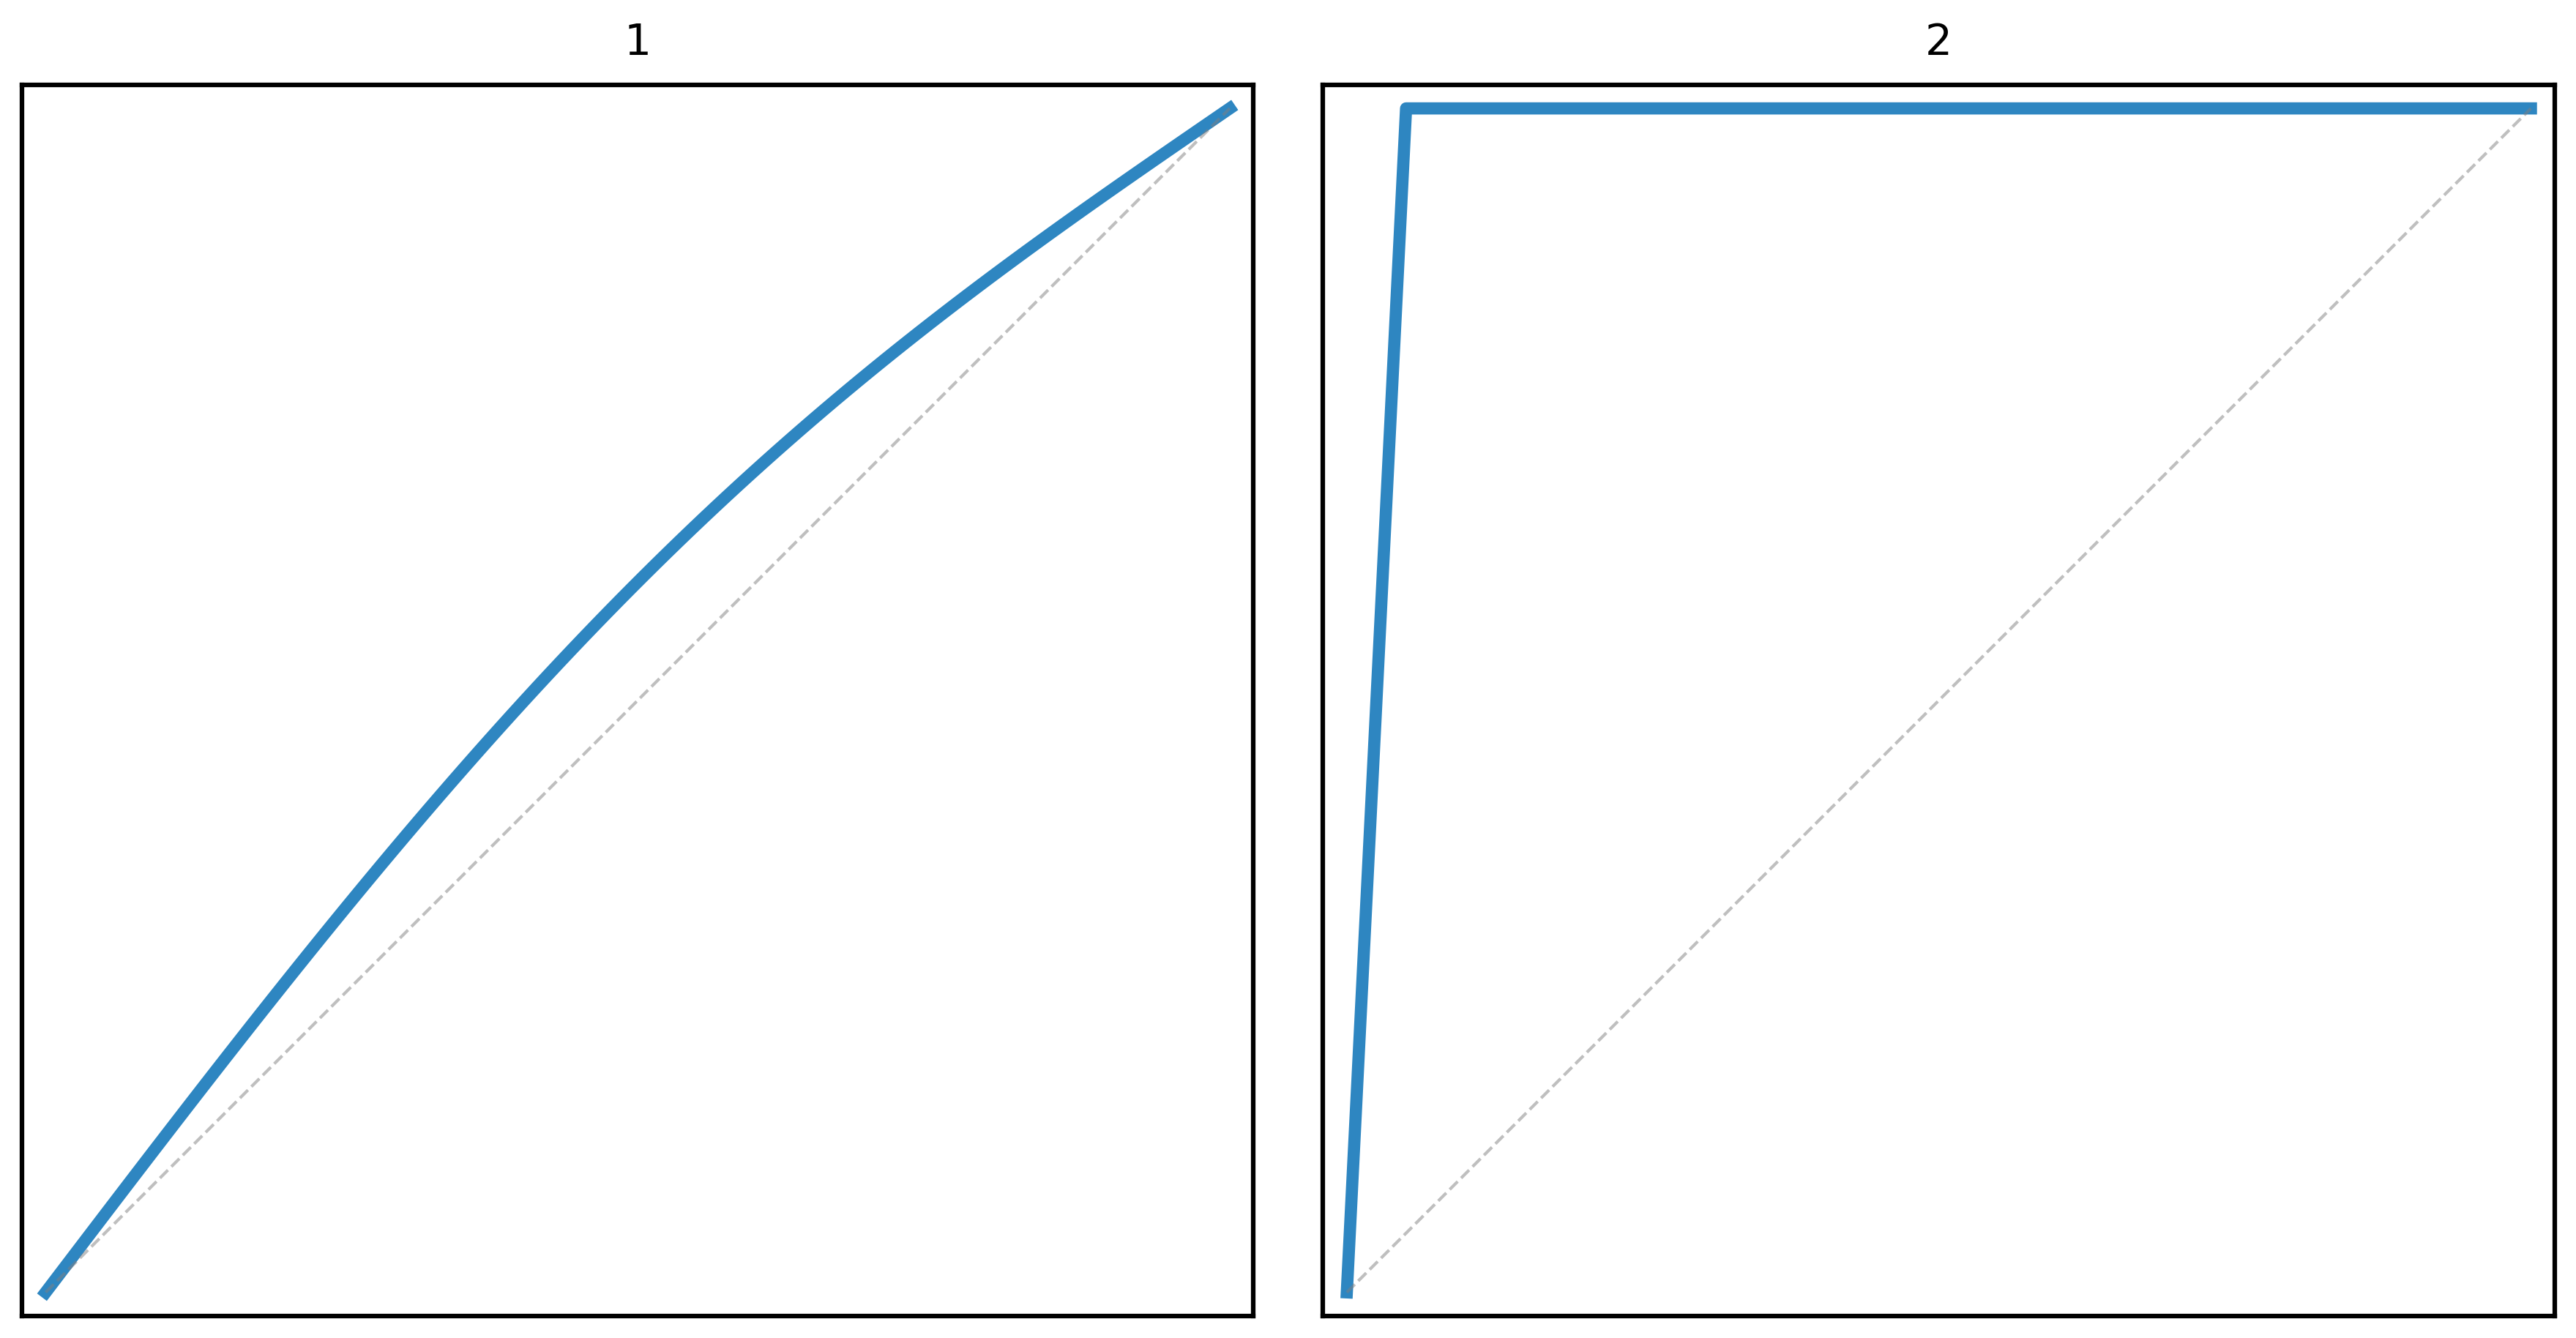
\includegraphics[width=0.8\textwidth]{chapters/feature_selection/roc_curves_comparison_1.png}
    \caption{Две ROC кривые}
\end{figure}
Как эти модели упорядочить по качеству?

\subsection*{Решение}
Первая модель самая худшая, ведь ее ROC кривая максимально близка к диагонали, значит она имеет миниимальную ROC-AUC.
Это плохо, но что по смыслу означает близкая к диагонали ROC кривая?

Это означает, что для любого порога отсечения $t$ имеем примерно $TPR(t) = FPR(t)$.
Что означает $TPR(t) = FPR(t)$? Это означает, что модель просто случайным образом с вероятностью $TPR(t)=FPR(t)$ предсказывает 1 класс.
Вторая модель лучшая, но почему?

А что означает график, который близок к уголку, как на рисунке 2?
Это означает, что мы можем взять такой порог отсечения $t$, что почти выполнено $TPR(t) = 1$ и $FPR(t) = 0$.
А это идеальная модель, которая никогда не ошибается.

Заметим, что чем больше площадь под ROC кривой, тем ближе эта кривая к уголку, а значит тем лучше модель.

\subsection*{Задача 3}
Продолжим измерять качество моделей с помощью ROC-AUC. Допустим, что у нас есть две модели, чьи ROC кривые выглядят следующим образом:
\begin{figure}[h]
    \centering
    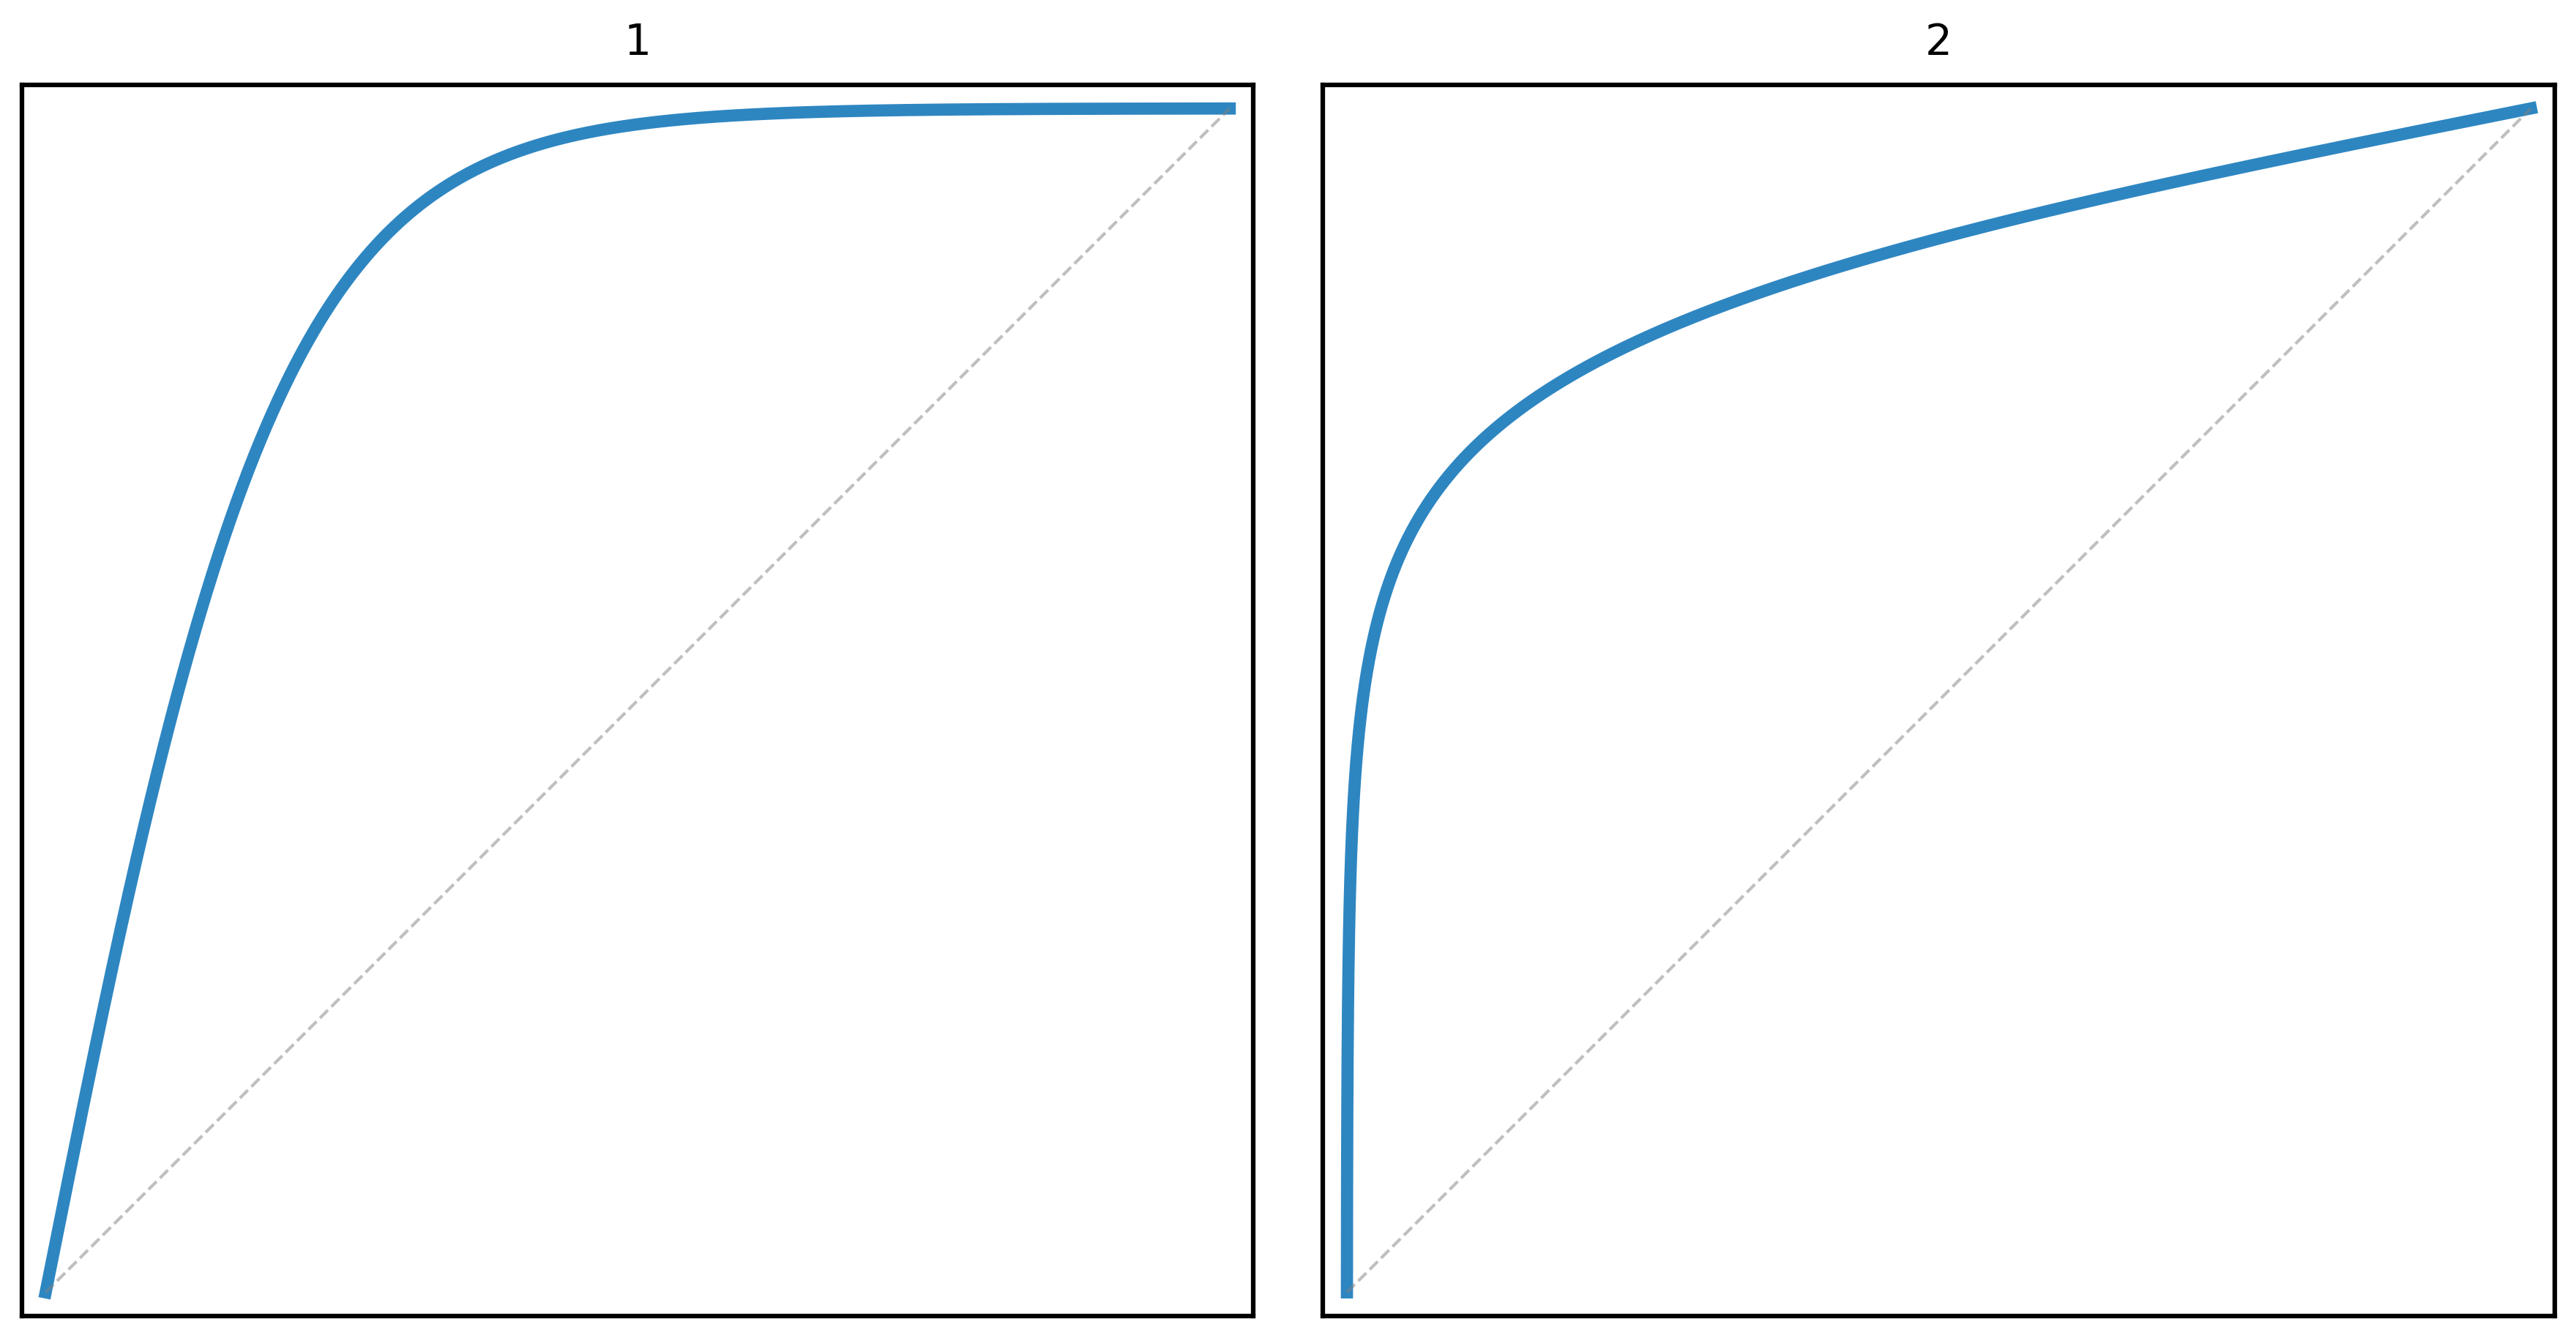
\includegraphics[width=0.8\textwidth]{chapters/feature_selection/roc_curves_comparison_2.png}
    \caption{Две ROC кривые}
\end{figure}
Как эти модели упорядочить по качеству? А как выбрать порог отсечения? В чем преимущество ROC перед $F_{\beta}$ score?

\subsection*{Решение}
В данном случае, обе ROC кривые имеют одинаковую площадь под графиком, а значит одинаковую ROC-AUC, поэтому просто посмотреть на метрику ROC-AUC нельзя.
На самом деле, однозначного ответа нет, всё зависит от конкретной задачи.

Первая кривая быстро достигает высокого значения TPR, при не самом высоком значении FPR.

Это означает, что выбрав порог отсечения $t$, при котором $TPR(t)$ будет близок к 1, а $FPR(t)$ будет близок к 0.5, мы получим модель,
которая угадывает почти всех, кто попадает в 1 класс, но при этом не сильно много ошибается на классе 0.
Такая модель отлично подойдет в первой задаче, где мы хотим отгадать почти всех больных, но при этом не сильно много отправлять на дополнительное обследование здоровых людей.

На втором графике ситуация обратная, мы можем выбрать порог отсечения $t$, при котором $TPR(t)$ будет близок к 0.5, а $FPR(t)$ будет близок к 1.
Такая модель будет полезна в случае, когда мы хотим минимизировать количество ошибок на классе 0, но при этом не сильно много ошибаться на классе 1.
В контексте первой задачи, это означает, что мы не хотим тратить лишние деньги на дополнительное обследование здоровых людей даже ценой смерти больных, которых мы не отправляем на дополнительное обследование.

Исходя из этих примеров, становится понятно, как стоит выбирать порог отсечения. По сути его выбор означает, насколько мы готовы пожертвовать ошибками на предсказаниях одного класса, чтобы минимизировать ошибки на предсказаниях другого класса.
Это такой аналог $\beta$ в $F_{\beta}$ score, только $\beta$ мы выбирали до измерения метрики, а в случае ROC кривой мы выбираем порог отсечения глядя на график и имея какую-то дополнительную информацию о том, как работает модель при разных порогах.
Это может быть очень полезно, ведь далеко не всегда мы готовы определиться с балансом ошибок на классах перед тем, как начать решать задачу.


\section*{Отбор признаков: алгоритм Add-Del}

Отбор признаков — это важный этап работы с данными в машинном обучении. Его цель — выбрать подмножество признаков, которые наиболее значимы для построения качественной модели. Используя разные методы отбора признаков, мы можем улучшить производительность модели, сократить время обучения и избежать переобучения. 




\subsection*{Алгоритм Add-Del (Stepwise Selection)}

Этот жадный метод объединяет добавление и удаление признаков. Он пытается улучшить результат, проверяя, можно ли удалить ранее добавленные признаки.

\subsubsection*{План действий}

\begin{enumerate}

\item Начинаем с пустого набора (или с начального набора признаков).

\item Добавление признаков: находим и добавляем тот признак, который максимизирует качество модели.

\item Удаление признаков: после добавления нового признака проверяется, можно ли удалить какой-либо из уже добавленных без ухудшения качества модели.

\item Шаги повторяются, пока не перестанет улучшаться метрика или не будут обработаны все признаки.

\end{enumerate}


\subsubsection*{Алгоритм}


Инициализация:
\[
J_0 := \emptyset; \quad Q^* := Q(\emptyset); \quad t := 0;
\]

\textbf{Повторять:}
\begin{itemize}
    \item Пока \( |J_t| < n \), добавлять признаки (итерации Add):
    \begin{itemize}
        \item \( t := t + 1 \) — началась следующая итерация;
        \item Найти признак:
        \[
        f^* := \arg \min_{f \in F \setminus J_{t-1}} Q(J_{t-1} \cup \{f\});
        \]
        \item Добавить признак:
        \[
        J_t := J_{t-1} \cup \{f^*\};
        \]
        \item Если \( Q(J_t) < Q^* \), то:
        \[
        t^* := t; \quad Q^* := Q(J_t);
        \]
        \item Если \( t - t^* \geq d \), то прервать цикл.
    \end{itemize}
    \item Пока \( |J_t| > 0 \), удалять признаки (итерации Del):
    \begin{itemize}
        \item \( t := t + 1 \) — началась следующая итерация;
        \item Найти признак:
        \[
        f^* := \arg \min_{f \in J_{t-1}} Q(J_{t-1} \setminus \{f\});
        \]
        \item Удалить признак:
        \[
        J_t := J_{t-1} \setminus \{f^*\};
        \]
        \item Если \( Q(J_t) < Q^* \), то:
        \[
        t^* := t; \quad Q^* := Q(J_t);
        \]
        \item Если \( t - t^* \geq d \), то прервать цикл.
    \end{itemize}
\end{itemize}

\textbf{Пока значения критерия \( Q(J_{t^*}) \) уменьшаются:}

\[ \text{Вернуть} \ ( J_{t^*} ).\]


\begin{figure}[h!!!!!!!!!!]
	\centering
	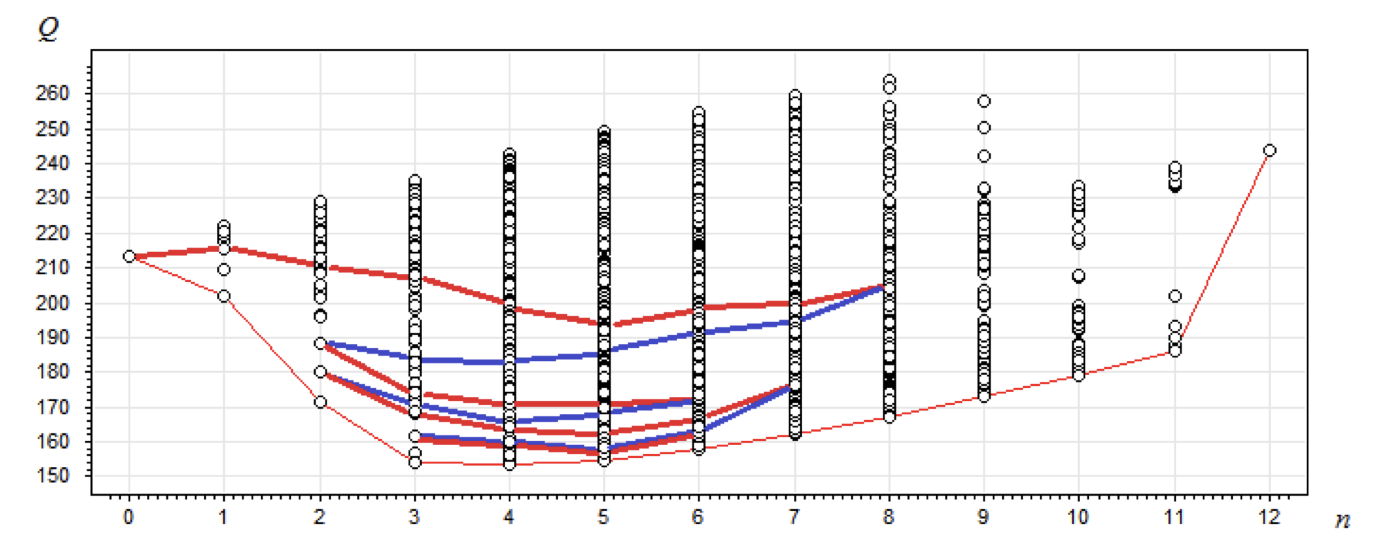
\includegraphics[width=1\linewidth]{add-del.png}
\end{figure}



\subsubsection*{Преимущества}

\begin{itemize}

    \item Как правило лучше, чем Add и Del по отдельности, и болле гибкий, чем полный перебор

    \item Может устранить незначимые признаки, которые случайно попали в набор
    
\end{itemize}

\subsubsection*{Недостатки}

\begin{itemize}

    \item Еще медленнее, чем полный перебор

    \item Не гарантирует оптимальность
    
\end{itemize}



\bigskip
\bigskip




\subsection*{Задачи}



\subsubsection*{Задача 1. Применение алгоритма Add-Del}

Рассмотрим множество признаков \( F = \{f_1, f_2, f_3, f_4\} \) и следующую таблицу значений критерия \( Q(J) \) для различных наборов признаков \( J \):

\[
\begin{array}{|c|c|}
\hline
J & Q(J) \\
\hline
\emptyset & 10 \\
\{f_1\} & 8 \\
\{f_2\} & 9 \\
\{f_3\} & 6 \\
\{f_4\} & 7 \\
\{f_1, f_2\} & 7.5 \\
\{f_1, f_3\} & 5.5 \\
\{f_1, f_4\} & 6.5 \\
\{f_2, f_3\} & 6.2 \\
\{f_2, f_4\} & 6.8 \\
\{f_3, f_4\} & 5.2 \\
\{f_1, f_2, f_3\} & 5.0 \\
\{f_1, f_2, f_4\} & 5.7 \\
\{f_1, f_3, f_4\} & 4.8 \\
\{f_2, f_3, f_4\} & 5.1 \\
\{f_1, f_2, f_3, f_4\} & 5.2 \\
\hline
\end{array}
\]

Примените алгоритм Add-Del с параметром \( d = 2 \), начиная с пустого множества. Найдите итоговый набор признаков \( J_{t^*} \), при котором значение критерия \( Q \) минимально.

\bigskip

\textbf{Решение}



\begin{enumerate}


\item \textbf{Инициализация}:
\[
J_0 := \emptyset, \quad Q^* := Q(\emptyset) = 10, \quad t := 0.
\]

\item \textbf{Итерации Add}:
\begin{itemize}
    \item \textbf{Итерация 1}: 
    \[
    t = 1, \quad f^* = \arg \min_{f \in F \setminus J_0} Q(J_0 \cup \{f\}) = f_3, \quad Q(J_1) = Q(\{f_3\}) = 6.
    \]
    \[
    J_1 = \{f_3\}, \quad Q^* = 6, \quad t^* = 1.
    \]

    \item \textbf{Итерация 2}: 
    \[
    t = 2, \quad f^* = \arg \min_{f \in F \setminus J_1} Q(J_1 \cup \{f\}) = f_4, \quad Q(J_2) = Q(\{f_3, f_4\}) = 5.2.
    \]
    \[
    J_2 = \{f_3, f_4\}, \quad Q^* = 5.2, \quad t^* = 2.
    \]

    \item \textbf{Итерация 3}: 
    \[
    t = 3, \quad f^* = \arg \min_{f \in F \setminus J_2} Q(J_2 \cup \{f\}) = f_1, \quad Q(J_3) = Q(\{f_3, f_4, f_1\}) = 4.8.
    \]
    \[
    J_3 = \{f_3, f_4, f_1\}, \quad Q^* = 4.8, \quad t^* = 3.
    \]

    \item \textbf{Итерация 4}: 
    \[
    t = 4, \quad f^* = \arg \min_{f \in F \setminus J_3} Q(J_3 \cup \{f\}) = f_2, \quad Q(J_4) = Q(\{f_3, f_4, f_1, f_2\}) = 5.2.
    \]
    \[
    J_4 = \{f_3, f_4, f_1, f_2\}.
    \]
    Здесь \( Q(J_4) \geq Q^* \), но \( t - t^* = 1 < d \), поэтому продолжаем.

    \item \textbf{Итерация 5}: 
    \[
    t = 5.
    \]
    Поскольку \( t - t^* = 2 \geq d \), прерываем цикл Add.
\end{itemize}

\item \textbf{Итерации Del}:
\begin{itemize}
    \item \textbf{Итерация 1}: 
    \[
    t = 6, \quad f^* = \arg \min_{f \in J_4} Q(J_4 \setminus \{f\}) = f_2, \quad Q(J_5) = Q(\{f_3, f_4, f_1\}) = 4.8.
    \]
    \[
    J_5 = \{f_3, f_4, f_1\}, \quad Q^* = 4.8, \quad t^* = 6.
    \]

    \item \textbf{Итерация 2}: 
    \[
    t = 7, \quad f^* = \arg \min_{f \in J_5} Q(J_5 \setminus \{f\}) = f_1, \quad Q(J_6) = Q(\{f_3, f_4\}) = 5.2.
    \]
    \[
    J_6 = \{f_3, f_4\}.
    \]
    Здесь \( Q(J_6) > Q^* \), но \( t - t^* = 1 < d \), продолжаем.

    \item \textbf{Итерация 3}: 
    \[
    t = 8.
    \]
    Поскольку \( t - t^* = 2 \geq d \), прерываем цикл Del.
\end{itemize}

\item \textbf{Результат}:

Итоговый набор признаков:
\[
J_{t^*} = \{f_3, f_4, f_1\}.
\]

\end{enumerate}

Ответ: минимальное значение критерия: $Q^* = 4.8$.




\bigskip



\subsubsection*{Задача 2. Алгоритм Add-Del для максимизации \( Q(J) \)}

У вас есть множество признаков \( F = \{f_1, f_2, f_3, f_4, f_5\} \). Для каждого признака известно его качество (чем выше, тем лучше) и стоимость (чем ниже, тем лучше). Данные представлены в таблице:

\[
\begin{array}{|c|c|c|}
\hline
\text{Признак} & \text{Качество} & \text{Стоимость} \\
\hline
f_1 & 7 & 4 \\
f_2 & 5 & 2 \\
f_3 & 9 & 5 \\
f_4 & 8 & 6 \\
f_5 & 6 & 3 \\
\hline
\end{array}
\]

Критерий \( Q(J) \) для набора \( J \) определяется как:  
\[
Q(J) = \frac{\sum_{f \in J} \text{качество}(f)}{\sum_{f \in J} \text{стоимость}(f) + |J|}.
\]

Чем выше значение \( Q(J) \), тем лучше набор. Используйте алгоритм \textbf{Add-Del} с параметром \( d = 1 \), чтобы найти набор признаков, который максимизирует \( Q(J) \). Начальное множество \( J_0 \) пусто.

\bigskip



\textbf{Решение}

\begin{enumerate}

\item \textbf{Инициализация}
\[
J_0 := \emptyset, \quad Q^* := 0, \quad t := 0.
\]

\item \textbf{Итерации Add}

\textbf{Шаг 1: \( t = 1 \)}
Рассматриваем добавление каждого признака \( f \in F \):  
\[
\begin{aligned}
Q(\{f_1\}) & = \frac{7}{4 + 1} = 1.4, \\
Q(\{f_2\}) & = \frac{5}{2 + 1} = 1.67, \\
Q(\{f_3\}) & = \frac{9}{5 + 1} = 1.5, \\
Q(\{f_4\}) & = \frac{8}{6 + 1} = 1.14, \\
Q(\{f_5\}) & = \frac{6}{3 + 1} = 1.5.
\end{aligned}
\]

Выбираем \( f^* = f_2 \), так как \( Q(\{f_2\}) \) максимально.  
Обновляем:  
\[
J_1 := \{f_2\}, \quad Q^* := 1.67.
\]

\textbf{Шаг 2: \( t = 2 \)}
Рассматриваем добавление признаков \( f \in F \setminus J_1 = \{f_1, f_3, f_4, f_5\} \):  
\[
\begin{aligned}
Q(\{f_2, f_1\}) & = \frac{5 + 7}{2 + 4 + 2} = \frac{12}{8} = 1.5, \\
Q(\{f_2, f_3\}) & = \frac{5 + 9}{2 + 5 + 2} = \frac{14}{9} = 1.56, \\
Q(\{f_2, f_4\}) & = \frac{5 + 8}{2 + 6 + 2} = \frac{13}{10} = 1.3, \\
Q(\{f_2, f_5\}) & = \frac{5 + 6}{2 + 3 + 2} = \frac{11}{7} = 1.57.
\end{aligned}
\]

Выбираем \( f^* = f_5 \), так как \( Q(\{f_2, f_5\}) \) максимально.  
Обновляем:  
\[
J_2 := \{f_2, f_5\}, \quad Q^* := 1.57.
\]

\item \textbf{Итерации Del}

\textbf{Шаг 3: \( t = 3 \)}
Рассматриваем удаление признаков из \( J_2 = \{f_2, f_5\} \):  
\[
\begin{aligned}
Q(\{f_5\}) & = \frac{6}{3 + 1} = 1.5, \\
Q(\{f_2\}) & = \frac{5}{2 + 1} = 1.67.
\end{aligned}
\]

Удаление признака \( f_5 \) не улучшает \( Q^* \). Цикл завершается.

\item \textbf{Результат}

Итоговый набор:  
\[
J_{t^*} = \{f_2, f_5\}, \quad Q^* = 1.57.
\]

\end{enumerate}





\bigskip

\subsubsection*{Задача 3. Оптимизация алгоритма Add-Del с ограничением на размер набора признаков}

\textbf{Условие:}

Рассмотрим 6 признаков $F = \{x_1, x_2, x_3, x_4, x_5, x_6\}$ и известные значения функции ошибки $Q(J)$ для некоторых подмножеств. Установлено, что $Q(J)$ вычисляется по следующему правилу:
\[
Q(J) = 20 - 3|J| + \sum_{i \in J} w_i,
\]
где веса $w_i$ для признаков заданы следующим образом:
\[
w_1 = 5, \, w_2 = 3, \, w_3 = 2, \, w_4 = 1, \, w_5 = 1, \, w_6 = 0.
\]

Пусть максимальное допустимое количество признаков в итоговом наборе равно 4, то есть $|J| \leq 4$. Используя алгоритм Add-Del:
\begin{enumerate}
    \item Найдите итоговый набор признаков $J$.
    \item Объясните, на каком шаге и почему применяется удаление признаков.
    \item Сравните итоговый результат Add-Del с Add.
\end{enumerate}

\textbf{Решение:}

\begin{enumerate}
    \item На начальном этапе множество признаков $J = \emptyset$, и $Q(\emptyset) = 20$.
    \item Алгоритм Add:
    \begin{itemize}
        \item Добавляем $x_4$, так как $w_4 = 1$ минимально, получаем $J = \{x_4\}$, $Q(J) = 20 - 3 \cdot 1 + 1 = 18$.
        \item Добавляем $x_5$, так как $w_5 = 1$, получаем $J = \{x_4, x_5\}$, $Q(J) = 20 - 3 \cdot 2 + 1 + 1 = 16$.
        \item Добавляем $x_6$, так как $w_6 = 0$, получаем $J = \{x_4, x_5, x_6\}$, $Q(J) = 20 - 3 \cdot 3 + 1 + 1 + 0 = 14$.
        \item Добавляем $x_3$, так как $w_3 = 2$, получаем $J = \{x_4, x_5, x_6, x_3\}$, $Q(J) = 20 - 3 \cdot 4 + 1 + 1 + 0 + 2 = 12$.
    \end{itemize}
    Итоговый набор после алгоритма Add: $J = \{x_4, x_5, x_6, x_3\}$.

    \item Алгоритм Add-Del:
    \begin{itemize}
        \item Следуя тем же шагам Add, находим $J = \{x_4, x_5, x_6, x_3\}$, $Q(J) = 12$.
        \item Проверяем возможность удаления признаков:
        \begin{itemize}
            \item Удаляем $x_3$, так как $Q(\{x_4, x_5, x_6\}) = 20 - 3 \cdot 3 + 1 + 1 + 0 = 14$, что хуже текущего значения $Q(J)$.
            \item Удаляем $x_5$, получаем $Q(\{x_4, x_6, x_3\}) = 20 - 3 \cdot 3 + 1 + 0 + 2 = 13$, что тоже хуже.
        \end{itemize}
    \end{itemize}
    Итоговый набор совпадает с Add: $J = \{x_4, x_5, x_6, x_3\}$, $Q(J) = 12$.
    
    \item Сравнение Add и Add-Del:
    \begin{itemize}
        \item Алгоритмы Add и Add-Del дают одинаковый результат, так как все удаленные подмножества не улучшили $Q$.
        \item Однако Add-Del более устойчив к ошибкам из-за возможности отката.
    \end{itemize}
\end{enumerate}

\section{Методы отбора признаков: полный перебор, алгоритм Add}

Работа с признаками включает два основных подхода:
\begin{enumerate}
    \item Генерация новых признаков;
    \item Отбор существующих признаков.
\end{enumerate}

\subsection{Генерация новых признаков}
Генерация новых признаков подразумевает создание таких признаков, которые представляют собой преобразованные версии исходных данных или полностью новые параметры, полученные из имеющихся данных. Примеры методов генерации признаков включают:

\begin{itemize}
    \item Построение статистик на основе существующих признаков (например, среднее, стандартное отклонение, медиана и т.д.);
    \item Использование методов понижения размерности, таких как анализ главных компонент (PCA);
    \item Применение нейросетей, где скрытые слои (за исключением последнего) могут рассматриваться как новое, более информативное признаковое пространство.
\end{itemize}

В этой главе мы сосредоточимся на отборе существующих признаков, рассмотрев два наиболее популярных метода: полный перебор и жадный алгоритм Add.

\subsection{Полный перебор}

Метод полного перебора представляет собой один из самых простых и технически точных подходов к отбору признаков. Суть метода заключается в оценке качества модели на всех возможных комбинациях признаков и выборе той комбинации, которая обеспечивает наилучшую метрику. Таким образом, полный перебор \textbf{гарантирует нахождение оптимального набора признаков}, так как проверяет все возможные варианты.

Основное преимущество полного перебора заключается в его точности: при достаточных вычислительных ресурсах метод всегда найдёт лучшее решение. Тем не менее, с увеличением числа признаков $n$, количество возможных подмножеств растёт экспоненциально ($2^n$). Это делает полный перебор крайне ресурсоёмким для наборов данных с большим $n$. Например, уже при $n=20$ потребуется рассчитать $2^{20} = 1,048,576$ комбинаций.

Метод полного перебора чаще применяется:
\begin{itemize}
    \item Для небольших наборов признаков, где перебор возможен за приемлемое время;
    \item В задачах, где цена ошибки высока (например, в медицинских исследованиях);
    \item Когда требуется хорошая интерпретируемость и точность подмножеств признаков.
\end{itemize}

На больших данных иногда применяются модификации полного перебора, такие как частичный перебор, где анализируется только часть комбинаций (например, сначала отбираются наиболее значимые признаки с помощью другого метода, а затем производится перебор подмножеств только из этих признаков).

\subsection{Жадный алгоритм Add}

Алгоритм Add (жадный подход) используется гораздо чаще, чем полный перебор, благодаря лучшей производительности на больших данных и более простой интерпретации. Суть метода заключается в пошаговом добавлении признаков в модель. На каждом шаге из оставшихся признаков выбирается тот, который обеспечивает наибольшее улучшение метрики модели. Таким образом, итоговый набор строится итеративно, начиная с пустого множества и поочередно добавляя наиболее значимые признаки.

Жадный алгоритм не гарантирует нахождения глобального оптимума, так как выбирает локально лучшие решения на каждом из шагов. Однако его высокая скорость и способность работать с большими наборами признаков делают его востребованным для многих задач.

Очевидно, что из общего числа признаков $n$ должен остаться некоторый $k$-подмножество наиболее значимых признаков. Критерии остановки алгоритма Add могут быть следующими:

\begin{itemize}
    \item \textbf{Фиксированное количество признаков $k$}:  
    Алгоритм останавливается, как только выбрано заданное количество признаков $k$.  
    \textit{Плюсы:} простота реализации и возможность заранее контролировать размерность данных.  
    \textit{Минусы:} фиксированное значение $k$ может оказаться избыточным в одной задаче или недостаточным в другой. Чтобы минимизировать неопределённость, значения параметра $k$ можно подбирать по сетке с помощью кросс-валидации.
    
    \item \textbf{Остановка при отсутствии улучшения метрики}:  
    На каждом шаге проверяется, насколько новая комбинация признаков улучшает метрику модели (например, \(R^2\), \(MAPE\), RMSE). Если добавление нового признака не приводит к значимому улучшению (или ухудшает метрику), алгоритм прекращает выполнение.  
    \textit{Плюсы:} гибкость метода, так как он адаптируется к конкретной задаче.  
    \textit{Минусы:} возможно преждевременное завершение, если данные содержат шум.
\end{itemize}

Метод Add применяется, когда требуется построить интерпретируемую модель с допустимым уровнем качества за ограниченное время. Например, алгоритм широко используется в финансах для выделения ключевых факторов прогнозирования прибыли или моделирования рисков, а также в обработке медицинских данных. 

\textbf{Преимущества метода Add:}
\begin{itemize}
    \item Высокая скорость работы и масштабируемость для большого числа признаков;
    \item Возможность построить достаточно простую и интерпретируемую модель.
\end{itemize}

\textbf{Недостатки метода Add:}
\begin{itemize}
    \item Чувствительность к входным данным: выбросы и избыточные признаки могут искажать отбор на ранних этапах;
    \item Отсутствие глобальной оптимальности: алгоритм может игнорировать комбинации признаков, т.к. учитывает только влияние признаков по отдельности.
\end{itemize}

\subsection{Задачи}

\subsubsection{Задача 1.}

Есть набор данных с N = 10000 признаков, и задача состоит в отборе важных признаков. Отбор происходит с помощью метода Add, но на каждом шаге анализ всех оставшихся признаков (выбор из 10000, затем из 9999 и т.д.) занимает слишком много времени.

Как можно было бы улучшить этот метод?

\subsubsection{Ответ 1.}

Можно разделить все признаки случайным образом на блоки (например, по 100 признаков). В таком случае хорошей идеей будет выбрать лучший признак из каждого блока на предварительном этапе (т.е. жадный Add выполняется на подмножествах сначала локально в блоках), а затем продолжить работу с меньшим числом представителей от каждых блоков. Если блоки и так большого размера, то можно воспользоваться этой идеей рекурсивно для каждого подблока.

\subsubsection{Задача 2.}

Рассмотрим использование жадного алгоритма Add для выбора признаков из набора данных с 5 признаками ({A, B, C, D, E}) в задаче классификации.

График перезаписи последовательного роста метрики $R^2$ при добавлении выбранных признаков показан ниже:

\begin{table}[h!]
\centering
\begin{tabular}{|c|c|c|}
\hline
\textbf{Итерация} & \textbf{Добавленный признак} & \boldmath${R^2}$ \\ \hline
1                 & $A$                       & 0.45             \\ \hline
2                 & $B$                       & 0.53             \\ \hline
3                 & $C$                       & 0.58             \\ \hline
\end{tabular}
\end{table}

Между тем, известна модель из полного перебора, где признаковая комбинация $({A, D, E})$ даёт $R^2 = 0.67$.

Почему метод Add мог не найти эту комбинацию? Как можно было бы исправить эту ситуацию и повысить вероятность нахождения глобального оптимума?

\subsubsection{Ответ 2.}

Жадный алгоритм Add выбирает признак на каждом шаге, который локально улучшает метрику максимально. Однако комбинация $({A, D, E})$ могла быть значимой только в сочетании (то есть признаки дают прирост метрики только в комбинации), а по отдельности эти фичи дают не такой хороший прирост к метрике, как $B$ и $C$. Add не проверяет взаимодействие признаков, поэтому выбор локально наилучших признаков $({A, B, C})$ мог игнорировать комбинацию, которая глобально лучше.

\textbf{Как с этим можно бороться?}
\begin{itemize}
    \item Проверять метрику при добавлении не одного признака, а пары/тройки/произвольного числа $m$ признаков.
    \item Использовать модификацию жадного алгоритма с дополнительными "прыжками", то есть, например, после 3 итераций Add можно сделать перезапуск среди лучших комбинаций 2 признаков.
\end{itemize}

\subsubsection{Вопрос 3.}

Есть набор данных с 20 признаками. Известно, что 10 из них абсолютно не связана с целевой переменной, т.е. являются шумовыми. Однако не известно, какие именно из них являются шумовыми. Для отбора признаков был применен жадный алгоритм Add.

Предположим, что на первых итерациях жадный алгоритм случайно выбрал несколько шумовых признаков, так как они хорошо улучшили метрику на обучающей выборке.

Как это повлияет на работу алгоритма Add в следующих итерациях? Какие подходы вы бы предложили, чтобы минимизировать вероятность включения шумовых признаков на ранних этапах?

\subsubsection{Ответ 3.}\

\textbf{1. Как это повлияет на дальнейшую работу алгоритма?}

Жадный алгоритм фиксирует признаки и рассматривает следующие шаги на основе текущего набора. Если шумовые признаки остаются в модели, они могут "вытеснять" более значимые признаки в дальнейших итерациях.
Итоговый результат может быть хуже, так как модель становится менее интерпретируемой и более склонной к переобучению на шум.

\textbf{2. Как можно минимизировать влияние шума на обучение?}

Для этого стоит перед алгоритмом применить другие фильтрационные методы для удаления явно нерелевантных признаков, например, убрать признаки, плохо коррелирующие с целевой переменной.

Также для этого можно попробовать применить кросс-валидацию при оценке каждого нового признака, чтобы убедиться, что он действительно улучшает модель (а не только улучшает метрику на обучающей выборке).

\section{Методы преобразования категориальных признаков}

Категориальные признаки (или категориальные переменные) — это тип данных, который представляет собой категории или группы. В отличие от количественных признаков, которые принимают числовые значения, категориальные признаки описывают качественные характеристики.

\begin{itemize}
	\item Номинальные признаки -- эти признаки представляют собой категории, которые не имеют никакого порядка (город, где проживает человек; цвет машины).
	\item Порядковые признаки -- эти признаки также представляют категории, но в отличие от номинальных, они имеют естественный порядок (уровень образования; степень удовлетворенности).
\end{itemize}

Такие признаки невозможно напрямую использовать в моделях машинного обучения, поскольку они работают с числами. Для решения этой проблемы есть различные методы.

\subsection*{One-hot (dummy) encoding}

One-hot encoding — это метод кодирования категориальных переменных, который преобразует каждую категорию в бинарный вектор, где только один элемент равен 1 (представляет категорию), а все остальные элементы равны 0.

Преимущества:
\begin{itemize}
	\item Он легко реализуется, а данные легко интерпретируются.
	\item Хорошо совместим почти со всеми алгоритмами.
	\item Подходит для изначально неупорядоченных данных.
\end{itemize}

Недостатки:
\begin{itemize}
	\item В случае большого количества категорий сильно увеличивает размерность, может привести к переобучению.
	\item Полученные признаки сильно разреженны, неэффективно по памяти и скорости вычислений.
	\item Не подходит для упорядоченных или взаимосвязанных данных.
\end{itemize}

\subsection*{Effect (treatment, deviation) encoding}

Effect encoding  — это метод кодирования категориальных переменных, который представляет каждую категорию в виде разности между средним значением целевой переменной и средними значениями для каждой категории. Этот метод позволяет учитывать информацию о влиянии каждой категории на целевую переменную.

Преимущества:
\begin{itemize}
	\item Сохраняет информацию о влиянии категории на целевую переменную.
	\item Не увеличивает размерность пространства признаков.
	\item Создает порядок между категориями, основываясь на значении целевой переменной.
\end{itemize}

Недостатки:
\begin{itemize}
	\item Не так прост для интерпретации, как one-hot encoding.
	\item Может создать многократную коллинеарность между несколькими категориальными признаками.
\end{itemize}

\subsection*{Label (ordinal) encoding}

Label encoding — это метод кодирования категориальных переменных, при котором каждой категории присваивается уникальное целочисленное значение.

Преимущества:
\begin{itemize}
	\item Прост в реализации.
	\item Не увеличивает размерность пространства признаков.
	\item Сохраняет информацию порядковых признаков.
	\item Хорошо совместим с алгоритмами, не зависящими от расстояния между значениями (деревья решений).
\end{itemize}

Недостатки:
\begin{itemize}
	\item Создает ложный порядок в номинальных признаках.
	\item Плохо совместим с линейными моделями.
	\item Создает ложные расстояния между категориями.
\end{itemize}

\subsection*{Count encoding}

Count encoding — это метод кодирования категориальных переменных, при котором каждой категории присваивается количество её появлений в наборе данных. 
	
Преимущества:
\begin{itemize}
	\item Прост в реализации.
	\item Сохраняет информацию о частоте.
	\item Не увеличивает размерность пространства признаков.
\end{itemize}

Недостатки:
\begin{itemize}
	\item Не сохраняет информацию порядковых признаков.
	\item Может создать коллинеарность для разных категорий с близкими частотами.
	\item Создает ложные расстояния между категориями.
\end{itemize}

\subsection*{Задача 1}

В случае использования one-hot encoding для категориального признака с $N$ уникальными значениями, мы получим $N$ новых признаков. Однако любой признак выражается через остальные, поскольку единица всегда стоит только в одном из них. То есть мы получили мультиколлинеарность, которая может ухудшить качества модели! Каким образом можно решить эту проблему?

\subsection*{Решение}

Самым простым решением будет просто удалить любой из полученных признаков. Мы избавимся от мультиколлинеарности и сохраним всю информацию о выборке.

\subsection*{Задача 2}

Проведите преобразование категориальных признаков по методу effective encoding:
\begin{table}[ht]
	\footnotesize
	\begin{tabular}{lllll}
		\hline
		Пробег, тыс. км & Цвет    & Год выпуска & Тип кузова & Стоимость, у.е. \\ \hline
		100             & Красный & 2015        & Хэтчбэк    & 10           \\
		10              & Зеленый & 2019        & Cедан      & 17           \\
		17              & Cиний   & 2022        & Cедан      & 18           \\
		150             & Красный & 2019        & Универсал  & 15           \\
		30              & Красный & 2023        & Хэтчбэк    & 20           \\
		174             & Cиний   & 2017        & Хэтчбэк    & 12           \\
		89              & Зеленый & 2017        & Хэтчбэк    & 14           \\ \hline
	\end{tabular}
\end{table}

\subsection*{Решение}

Для каждого цвета вычислим средние значение стоимости:
\begin{itemize}
	\item Красный: $r = \frac{10+15+20}{3}=15$.
	\item Зеленый: $g = \frac{17+14}{2}=15.5$.
	\item Синий: $b = \frac{18+9}{2}=13.5$.
\end{itemize}

Тогда среднее для всех признаков:
$$ avg = \frac{15 + 15.5 + 13.5}{3} = 14.66. $$

Значение нового признака, например, для красного цвета:
$$ r - avg = 0.33. $$

\begin{table}[ht]
	\footnotesize
	\begin{tabular}{lllllll}
		\hline
		Пробег, тыс. км & Цвет    & Год выпуска & Тип кузова & Цвет (eff) & Тип кузова (eff) & Стоимость, у.е. \\ \hline
		100             & Красный & 2015        & Хэтчбэк    & 0,33        & -2,00           & 10           \\
		10              & Зеленый & 2019        & Cедан      & 0,83        & 2,25            & 17           \\
		17              & Cиний   & 2022        & Cедан      & -1,16      & 2,25             & 18           \\
		150             & Красный & 2019        & Универсал  & 0,33        & -0.25             & 15           \\
		30              & Красный & 2023        & Хэтчбэк    & 0,33        & -2,00            & 20           \\
		174             & Cиний   & 2014        & Хэтчбэк    & -1,16      & -2,00            & 9            \\
		89              & Зеленый & 2017        & Хэтчбэк    & 0,83        & -2,00            & 14           \\ \hline
	\end{tabular}
\end{table}

\subsection*{Задача 3}

Предложите методы обработки пропущенных значений признаков.
Подсказка: можно основываться на некоторых методах преобразования категориальных признаков.

\subsection*{Решение}

Некоторые из возможных вариантов:
\begin{itemize}
	\item Добавление отдельного бинарного признака: есть/нет значение у исходного признака.
	\item Вычисление среднего по всем объектам с пропущенным значением исходного признака.
	\item Задание произвольных, не совпадающих с остальными, значений для каждого пропущенного значения исходного признака.
	\item Вычисление частоты пропущенных признаков.
\end{itemize}


    \clearpage
    \chapter{Логические методы классификации}
    \section{Бинаризация признаков}

Бинаризация признаков – это процесс преобразования исходных признаков в бинарные переменные, которые принимают значения \(0\) или \(1\). 
%Этот метод широко используется в задачах %машинного обучения, особенно в логических %методах классификации, где входные данные %должны быть представлены в виде набора %булевых предикатов.

\subsection{Бинаризация количественных признаков}

Для признака \( f: X \to D_f \), где \( D_f \) – множество возможных значений признака, бинаризация заключается в создании предикатов, проверяющих выполнение определённых условий. Эти предикаты позволяют разбить множество значений признака на подмножества, которые можно использовать в логических моделях.

В зависимости от типа признака, бинаризация осуществляется следующим образом:
\begin{itemize}
    \item \textbf{Номинальный признак} (\(f\) принимает конечное множество значений, без упорядоченности):
    \[
    \beta(x) = [f(x) = d], \quad d \in D_f;
    \]
    \[определитьопределить
    \beta(x) = [f(x) \in D'], \quad D' \subset D_f.
    \]
    \item \textbf{Порядковый или количественный признак} (\(f\) принимает значения, между которыми можно определить порядок):
    \[
    \beta(x) = [f(x) \leq d], \quad d \in D_f;
    \]
    \[
    \beta(x) = [d \leq f(x) \leq d'], \quad d, d' \in D_f, \, d < d'.
    \]
\end{itemize}

Для количественных признаков (\(f: X \to \mathbb{R}\)) важно выбирать такие пороговые значения \(d\), которые разделяют выборку на значимые группы. Например, 
%пороги \(d\) могут быть определены как средние значения между %соседними элементами вариационного ряда \(f(x_1), \dots, %f(x_\ell)\), упорядоченного по возрастанию:
\[
d_i = \frac{f^{(i)} + f^{(i+1)}}{2}, \quad f^{(i)} \neq f^{(i+1)}, \; i = 1, \dots, \ell - 1,
\]
где \(f^{(1)} \leq f^{(2)} \leq \dots \leq f^{(\ell)}\) – упорядоченные значения признака. (См. рис)

Такими способами можно получить много разных предикатов. Мы хотим выбрать из них самые ''лучшие'' (в каком-либо смысле). Для этого разобьем диапазон значений признака на зоны.

\begin{figure}
    \centering
    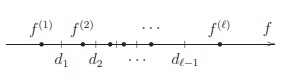
\includegraphics[scale = 1]{chapters/logical/images/bin1.png}
    \caption{Вариационный ряд значений признака $f(x)$ и пороги $d_i$}
\end{figure}

\subsection{Разбиение диапазона значений признака на зоны}

Каждая зона определяется бинарным предикатом:
\begin{align*}
\zeta_0(x) &= [f(x) < d_1], \\
\zeta_s(x) &= [d_s \leq f(x) < d_{s+1}], \quad s = 1, \dots, r-1, \\
\zeta_r(x) &= [d_r \leq f(x)].
\end{align*}

Способы разбиения:
\begin{itemize}
    \item Жадная максимизация информативности путем слияний
    \item Разбиение на равномощные подвыборки
    \item Разбиение по равномерной сетке ''удобных'' значений (например, с минимальным числом значащих цифр)
    \item Объединение нескольких разбиений
\end{itemize}

\subsection{Жадный алгоритм слияния зон}

Алгоритм начинает с разбиения на ''мелкие'' зоны. Пороги проходят между всеми соседними парами точек, принадлежащих \emph{разным} классам, т.~к. расстановка порогов между точками одного класса приведет только к уменьшению информативности зон. Далее зоны укрупняются путём слияния \emph{троек} соседних зон. Зоны сливаются до тех пор, пока
информативность некоторой слитой зоны превышает информативность
исходных зон, либо пока не будет получено заданное количество зон $r$. Каждый раз сливается тройка, дающая наибольший выигрыш в информативности.

\begin{figure}
    \centering
    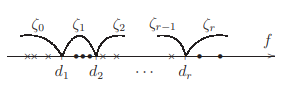
\includegraphics[scale = 1]{chapters/logical/images/bin2.png}
    \caption{Начальное разбиение на зоны}
\end{figure}

\newpage
\textbf{Вход:}
\begin{itemize}
    \item $f(x)$ — признак;
    \item $c \in Y$ — выделенный класс;
    \item $X^\ell = \{(x_i, y_i)\}_{i=1}^\ell$ — выборка, упорядоченная по возрастанию $f(x_i)$;
    \item $r$ — желаемое количество зон;
    \item $\delta_0$ — порог слияния зон (по умолчанию $\delta_0 = 0$).
\end{itemize}

\textbf{Выход:}
\[
D = \{d_1, \dots, d_n\} \text{ — строго возрастающая последовательность порогов;}
\]

\hrule

\begin{enumerate}
    \item $D := \emptyset;$
    \item \textbf{для всех} $i = 2, \dots, \ell$:
    \begin{itemize}
        \item \textbf{если} $f(x_{i-1}) \neq f(x_i)$ и $[y_{i-1} = c] \neq [y_i = c]$ \textbf{то}
        \begin{itemize}
            \item добавить новый порог $d := \frac{f(x_{i-1}) + f(x_i)}{2}$ в конец последовательности $D$;
        \end{itemize}
    \end{itemize}
    \item \textbf{повторять}
    \begin{enumerate}
        \item \textbf{для всех} $d_i \in D, i = 1, \dots, |D| - 1$:
        \begin{itemize}
            \item вычислить выигрыш от слияния тройки соседних зон $\zeta_{i-1}, \zeta_i, \zeta_{i+1}$:
            \[
            \delta_i := I_c(\zeta_{i-1} \cup \zeta_i \cup \zeta_{i+1}) - \max\{I_c(\zeta_{i-1}), I_c(\zeta_i), I_c(\zeta_{i+1})\};
            \]
        \end{itemize}
        \item найти тройку зон, для которой слияние наиболее выгодно:
        \[
        i := \arg \max \delta_i;
        \]
        \item \textbf{если} $\delta_i > \delta_0$ \textbf{то}
        \begin{itemize}
            \item слить зоны $\zeta_{i-1}, \zeta_i, \zeta_{i+1}$, удалить пороги $d_i$ и $d_{i+1}$ из последовательности $D$;
        \end{itemize}
    \end{enumerate}
    \item \textbf{пока} $|D| > r + 1$.
\end{enumerate}

\subsection{Задачи}

\textbf{Задача 1}
Предположим, вы владелец интернет-магазина, и у вас есть данные о стоимости товаров и их популярности (популярен — \( 1 \), непопулярен — \( 0 \)). 
Для анализа спроса вы хотите разбить товары на ценовые зоны, чтобы лучше понять поведение покупателей.

Данные представлены в таблице:

\[
\begin{array}{|c|c|c|}
\hline
\text{№ товара} & \text{Цена товара (\$)} & \text{Популярность } y \\
\hline
1 & 10 & 1 \\
2 & 12 & 1 \\
3 & 15 & 0 \\
4 & 17 & 1 \\
5 & 20 & 0 \\
6 & 23 & 0 \\
7 & 25 & 1 \\
\hline
\end{array}
\]

Как алгоритм слияния зон первично разобьёт выборку на ценовые зоны?

\textbf{Решение}
Рассчитаем пороги:

\[
\begin{aligned}
&d_1 = \frac{12 + 15}{2} = 13.5, \\
&d_2 = \frac{15 + 17}{2} = 16.0, \\
&d_3 = \frac{17 + 20}{2} = 18.5, \\
&d_4 = \frac{23 + 25}{2} = 24.0
\end{aligned}
\]

На основе рассчитанных порогов получаем зоны:

\[
\begin{aligned}
&\zeta_0(x) = [\text{Цена} < 13.5], \\
&\zeta_1(x) = [13.5 \leq \text{Цена} < 16.0], \\
&\zeta_2(x) = [16.0 \leq \text{Цена} < 18.5], \\
&\zeta_4(x) = [29.0 \leq \text{Цена} < 24.0], \\
&\zeta_5(x) = [\text{Цена} \geq 24.0].
\end{aligned}
\]

\textbf{Задача 2}
Будут ли разбиения диапазона меняться в зависимости от класса, относительно которого они производятся? Как изменить алгоритм для получения ''универсального'' разбиения, учитывающего сразу все классы? 

\textbf{Решение}
Да, будут, т.~к. информативность зависит от класса. Нужно заменить критерий информативности многоклассовым критерием.

\textbf{Задача 3}
Какую сложность имеет алгоритм слияния зон? Как можно его ускорить?

\textbf{Решение}
Этот алгоритм имеет трудоёмкость $O(l^2)$. Его можно заметно ускорить, если на каждой итерации сливать не одну тройку зон, а $\tau l$ троек с достаточно большим выигрышем $\delta I_i$, при условии, что они не перекрываются. В этом случае трудоёмкость составляет $O(l / \sqrt{\tau})$.

\section{Взвешенное голосование правил}

Допустим, имеется консилиум экспертов, каждый член которого может допустить ошибку. Процедура голосования — это способ повышения качества принимаемых решений, при котором ошибки отдельных экспертов компенсируют друг друга.

Ранее принцип голосования применялся для построения композиций из произвольных алгоритмов классификации. Теперь рассмотрим композиции, состоящие из логических закономерностей.

\subsection{Принцип голосования}

Пусть для каждого класса $c \in Y$ построено множество логических закономерностей (правил), специализирующихся на различении объектов данного класса:

\[
R_c = \{ \varphi_{tc} : X \to \{0, 1\} \mid t = 1, \dots, T_c \}
\]

Считается, что если $\varphi_{tc}(x) = 1$, то правило $\varphi_{tc}$ относит объект $x \in X$ к классу $c$. Если же $\varphi_{tc}(x) = 0$, то правило воздерживается от классификации объекта $x$.

Алгоритм простого голосования (simple voting) подсчитывает долю правил в наборах $R_c$, относящих объект $x$ к каждому из классов:

\[
\Gamma_c(x) = \frac{1}{T_c} \sum_{t=1}^{T_c} \varphi_{tc}(x), \quad c \in Y,
\]

и относит объект $x$ к тому классу, за который подана наибольшая доля голосов:

\[
a(x) = \arg \max_{c \in Y} \Gamma_c(x).
\]

Если максимум достигается одновременно на нескольких классах, выбирается тот, для которого цена ошибки меньше.

Нормирующий множитель $\frac{1}{T_c}$ вводится для того, чтобы наборы с большим числом правил не перетягивали объекты в свой класс.

\subsection{Алгоритм взвешенного голосования}
Алгоритм взвешенного голосования (weighted voting, WV) действует более тонко, учитывая, что правила могут иметь различную ценность. Каждому правилу $\varphi_{tc}$ приписывается вес $\alpha_{tc} \geq 0$, и при голосовании берется взвешенная сумма голосов:

\[
\Gamma_c(x) = \sum_{t=1}^{T_c} \alpha_{tc} \varphi_{tc}(x), \quad \alpha_{tc} > 0.
\]

Веса нормируются на единицу:

\[
\sum_{t=1}^{T_c} \alpha_{tc} = 1, \quad \forall c \in Y.
\]

Поэтому функцию $\Gamma_c(x)$ называют также выпуклой комбинацией правил $\varphi_1, \dots, \varphi_{T_c}$. Очевидно, простое голосование является частным случаем взвешенного, когда веса одинаковы и равны $\frac{1}{T_c}$.

На первый взгляд, вес правила должен определяться его информативностью. Однако, важно также учитывать, насколько данное правило уникально. Если имеется 10 хороших, но одинаковых (или почти одинаковых) правил, их суммарный вес должен быть сравним с весом столь же хорошего правила, не похожего на все остальные. Таким образом, веса должны учитывать не только ценность правил, но и их различность.

Простой общий подход к настройке весов заключается в том, чтобы сначала найти набор правил $\{ \varphi_{tc}(x) \}$, затем принять их за новые (бинарные) признаки и построить в этом новом признаковом пространстве линейную разделяющую поверхность (кусочно-линейную, если $|Y| > 2$). Для этого можно использовать логистическую регрессию, однослойный персептрон или метод опорных векторов. Существуют и другие подходы. Например, в разделе 1.5.4 будет рассмотрен метод бустинга, в котором правила настраиваются последовательно, и для каждого правила сразу вычисляется его вес.

\subsection{Проблема диверсификации правил}
Голосующие правила должны быть существенно различны, иначе они будут бесполезны для классификации. Продолжая аналогию с консилиумом, заметим, что нет никакого смысла держать в консилиуме эксперта A, если он регулярно подсматривает решения у эксперта B.

Приведем простое теоретико-вероятностное обоснование принципа диверсификации, или повышения различности (diversity) правил \cite{14}. Пусть $X$ — вероятностное пространство, множество ответов $Y$ конечно. Введем случайную величину $M(x)$, равную перевесу голосов в пользу правильного класса; её называют также отступом (margin) объекта $x$ от границы классов:

\[
M(x) = \Gamma_c(x) - \Gamma_{\overline{c}}(x), \quad \Gamma_{\overline{c}}(x) = \max_{y \in Y \setminus \{c\}} \Gamma_y(x), \quad c = y^*(x).
\]

Если отступ положителен ($M(x) > 0$), то алгоритм голосования правильно классифицирует объект $x$. Предположим, что в среднем наш алгоритм классифицирует хотя бы немного лучше, чем наугад: $E[M] > 0$. Тогда можно оценить вероятность ошибки по неравенству Чебышева:

\[
P\{M < 0\} \leq P\{|E[M] - M| > E[M]\} \leq \frac{D_M}{(E[M])^2}.
\]

Отсюда вывод: для уменьшения вероятности ошибки необходимо максимизировать ожидание перевеса голосов $E[M]$ и минимизировать его дисперсию $D_M$. Для выполнения этих условий каждый объект должен выделяться примерно одинаковым числом правил. Обычно ни одно из правил не выделяет класс целиком, поэтому правила должны быть существенно различны, то есть выделять существенно различные подмножества объектов.

Неплохая эвристика, усиливающая различия между правилами и позволяющая равномернее выделять объекты обучения, используется в алгоритме CORAL \cite{12}. Сначала для фиксированного класса $c \in Y$ строится покрывающий набор правил точно так, как это делалось для решающих списков. Затем строится второй покрывающий набор, но при этом запрещается использовать признаки, часто входившие в закономерности первого набора. Поэтому второй набор неминуемо окажется отличным от первого. Затем запрещаются признаки, часто входившие в оба набора, и строится третий набор. И так далее, для каждого класса $c \in Y$.

\subsection{Отказы от классификации}
Возможны ситуации, когда ни одно из правил не выделяет классифицируемый объект $x$. Тогда алгоритм должен либо отказываться от классификации, либо относить объект к классу, имеющему наименьшую цену ошибки. Отказ алгоритма означает, что данный объект является нетипичным, не подпадающим ни под одну из ранее обнаруженных закономерностей. Вообще, обнаружение нетипичности (novelty detection) принято считать отдельным видом задач обучения по прецедентам, наряду с классификацией и кластеризацией. Способность алгоритмов отказываться от классификации нетипичных объектов во многих приложениях является скорее преимуществом, чем недостатком. В то же время, число отказов не должно быть слишком большим.

Итак, при построении алгоритмов взвешенного голосования правил возникает четыре основных вопроса:
\begin{itemize}
    \item Как построить много правил по одной и той же выборке?
    \item Как избежать повторов и построения почти одинаковых правил?
    \item Как избежать появления непокрытых объектов и обеспечить равномерное покрытие всей выборки правилами?
    \item Как определять веса правил при взвешенном голосовании?
\end{itemize}

Рассмотрим, как эти проблемы решаются в известных алгоритмах в следующих параграфах.

\subsection{Задачи}

\textbf{Задача 1: Алгоритм простого голосования}

Допустим, для класса $c \in Y$ существуют 10 правил, которые используют данные для классификации. Каждое правило возвращает 1 или 0 для объекта $x$. Если для объекта $x$ правила 3 и 7 верно классифицируют объект как класс $c$, а остальные возвращают 0, как будет рассчитана доля голосов для класса $c$?

\textbf{Решение:}  
Для класса $c$ доля голосов рассчитывается как сумма всех правил, которые классифицируют объект как класс $c$, делённая на общее количество правил. Если 10 правил, то:
\[
\Gamma_c(x) = \frac{1}{10} \left( 1 + 0 + 0 + 0 + 0 + 0 + 1 + 0 + 0 + 0 \right) = \frac{2}{10} = 0.2
\]
Таким образом, для объекта $x$ доля голосов для класса $c$ составит 0.2.

\textbf{Задача 2: Проблема с весами в алгоритме взвешенного голосования}

В алгоритме взвешенного голосования веса для каждого правила нормируются на единицу. Если для класса $c$ у нас есть 3 правила с весами $\alpha_1 = 0.5$, $\alpha_2 = 0.3$, и $\alpha_3 = 0.2$, как будет выглядеть итоговая сумма голосов $\Gamma_c(x)$, если объект $x$ классифицируется всеми тремя правилами как класс $c$?

\textbf{Решение:}  
Итоговая сумма голосов для класса $c$ рассчитывается по формуле:
\[
\Gamma_c(x) = \sum_{t=1}^{T_c} \alpha_{tc} \varphi_{tc}(x)
\]
где $\varphi_{tc}(x) = 1$, если правило классифицирует объект как класс $c$, и 0 в противном случае. Если все 3 правила классифицируют объект как $c$, то:
\[
\Gamma_c(x) = 0.5 + 0.3 + 0.2 = 1.0
\]

\textbf{Задача 3: Проблема диверсификации правил}

Какова вероятность ошибки при использовании алгоритма голосования, если все правила сильно похожи друг на друга (например, классифицируют одинаковые подмножества объектов)?

\textbf{Решение:}  
Если правила сильно похожи, то вероятность ошибки возрастает. В таких случаях, возможно, правило не будет существенно различать объекты, и алгоритм может ошибаться при классификации новых объектов. Чтобы уменьшить вероятность ошибки, правила должны быть разнообразными, то есть они должны выделять разные подмножества объектов. Для максимизации различий между правилами можно использовать метод, как в алгоритме CORAL, который строит покрывающие наборы правил, постепенно исключая часто встречающиеся признаки.

\textbf{Задача 4: Принцип диверсификации правил}

Пусть для объекта $x$ имеется 10 правил, из которых 8 классифицируют объект как класс $c$, а остальные 2 — как класс $d$. Какой отступ $M(x)$ будет при расчете вероятности правильной классификации?

\textbf{Решение:}  
Отступ для объекта $x$ определяется как разница между голосами для правильного класса и максимальным голосом для всех остальных классов:
\[
M(x) = \Gamma_c(x) - \Gamma_{\overline{c}}(x)
\]
Если из 10 правил 8 голосуют за класс $c$ (доля голосов $0.8$) и 2 — за класс $d$ (доля голосов $0.2$), то:
\[
M(x) = 0.8 - 0.2 = 0.6
\]
Если отступ положителен ($M(x) > 0$), то классификация будет правильной.

\textbf{Задача 5: Отказы от классификации}

Если для объекта $x$ не существует правила, которое его классифицирует, что должен делать алгоритм голосования? Как можно обработать такой случай?

\textbf{Решение:}  
В таком случае алгоритм может либо отказаться от классификации, либо отнести объект к классу с наименьшей ценой ошибки. Такой отказ от классификации часто называют обнаружением нетипичности (novelty detection), что является отдельной задачей в машинном обучении. Важно, чтобы количество отказов не было слишком большим, так как это может снизить эффективность алгоритма.


    \clearpage
    \chapter{Поиск ассоциативных правил}
    \section{Алгоритм FP-Growth}
Алгоритм FP-Growth был опубликован в 2005 году Кристианом Боргельтом, и до сих пор является передовым в поиске ассоциативных правил. Алгоритм APriory, работает за $O(nl\cdot 2^k)$, где $n$ - это число признаков, $l$ - число записей в базе, а $k$ - максимальный размер ассоциативного правила. В то же время FP-Growth работает за $O(nl + f(k, n))$.

Идея этого алгоритма лежит в создании бора всех наборов $\varphi$, который будет хранить всю информацию о частотах встречаемости наборов, благодаря чему нам не придётся каждый раз пробегать всю базу с целью подсчёта $\nu(\varphi)$
\newline\newline
Алгоритм состоит из двух этапов:
\begin{enumerate}
    \item Построение FP-дерева
    \item Построение списка ассоциативных правил
\end{enumerate}

\subsection{Построение FP-дерева}

\begin{figure}[h]
    \centering
    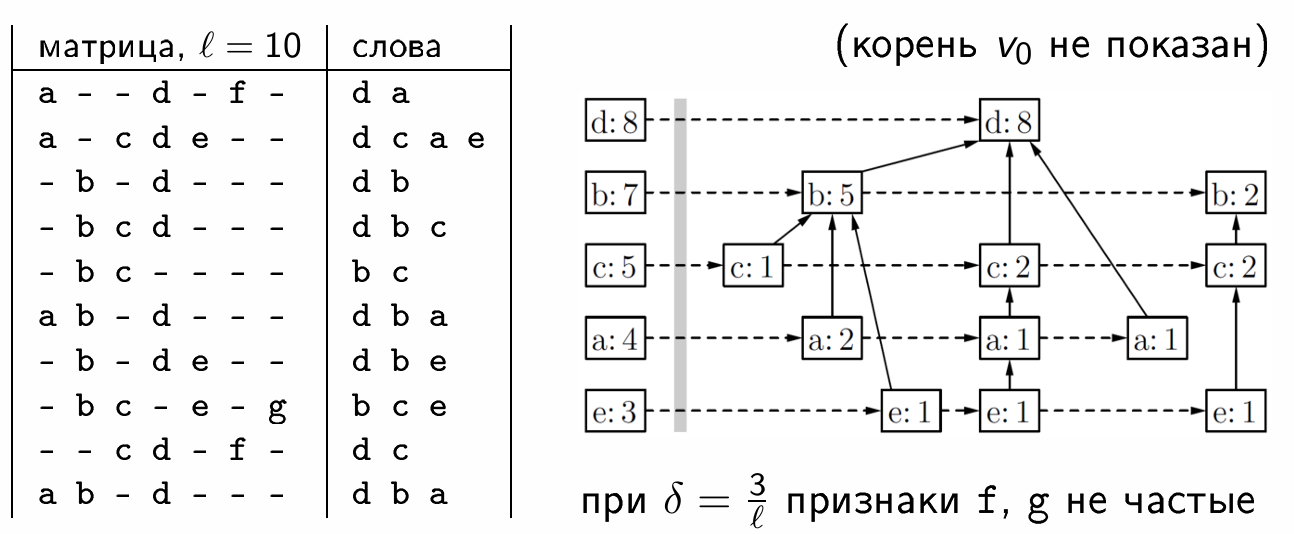
\includegraphics[width=0.8\linewidth]{chapters/metric/images/fp-tree-example.png}
    \caption{Пример FP-дерева}
\end{figure}

Первым делом упорядочим все признаки $f \in \mathcal{F}: \nu(f) \geq \delta$ по убыванию $\nu(f)$, их порядок будет соответствовать уровням вершин дерева (это не глубины!). Будем последовательно перебирать транзакции из базы. Будем хранить бор (FP-дерево), в каждой вершине $v$ которого будут храниться: 
\begin{enumerate}
    \item Признак $f_v \in \mathcal{F}$
    \item Множество дочерних вершин $S_v$
    \item Счетчик $c_v = \l\nu(\phi_v)$, где $\phi_v$ - набор состоящий из признаков соответствующих пути от корня до данной вершины. По сути этот счетчик равен количеству строк из базы, распознаваемых данной вершиной.
\end{enumerate}

Пусть для текущей транзакции $i$ положительны признаки из множества $F_i = \{f \in \mathcal{F}: f(x_i) = 1 \}$, упорядочим их по убыванию $\nu(f)$, получим строку $R_i$, начнем распознавать её бором. Если её нет в боре, создадим недостающие вершины, проинициализировав счетчики $c_{v_i} = 0$ в новых вершинах. Добавим 1 к счетчикам $c_v$ вершин, которые лежат на пути от корня, соответствующем $R_i$.

\begin{figure}[h]
    \centering
    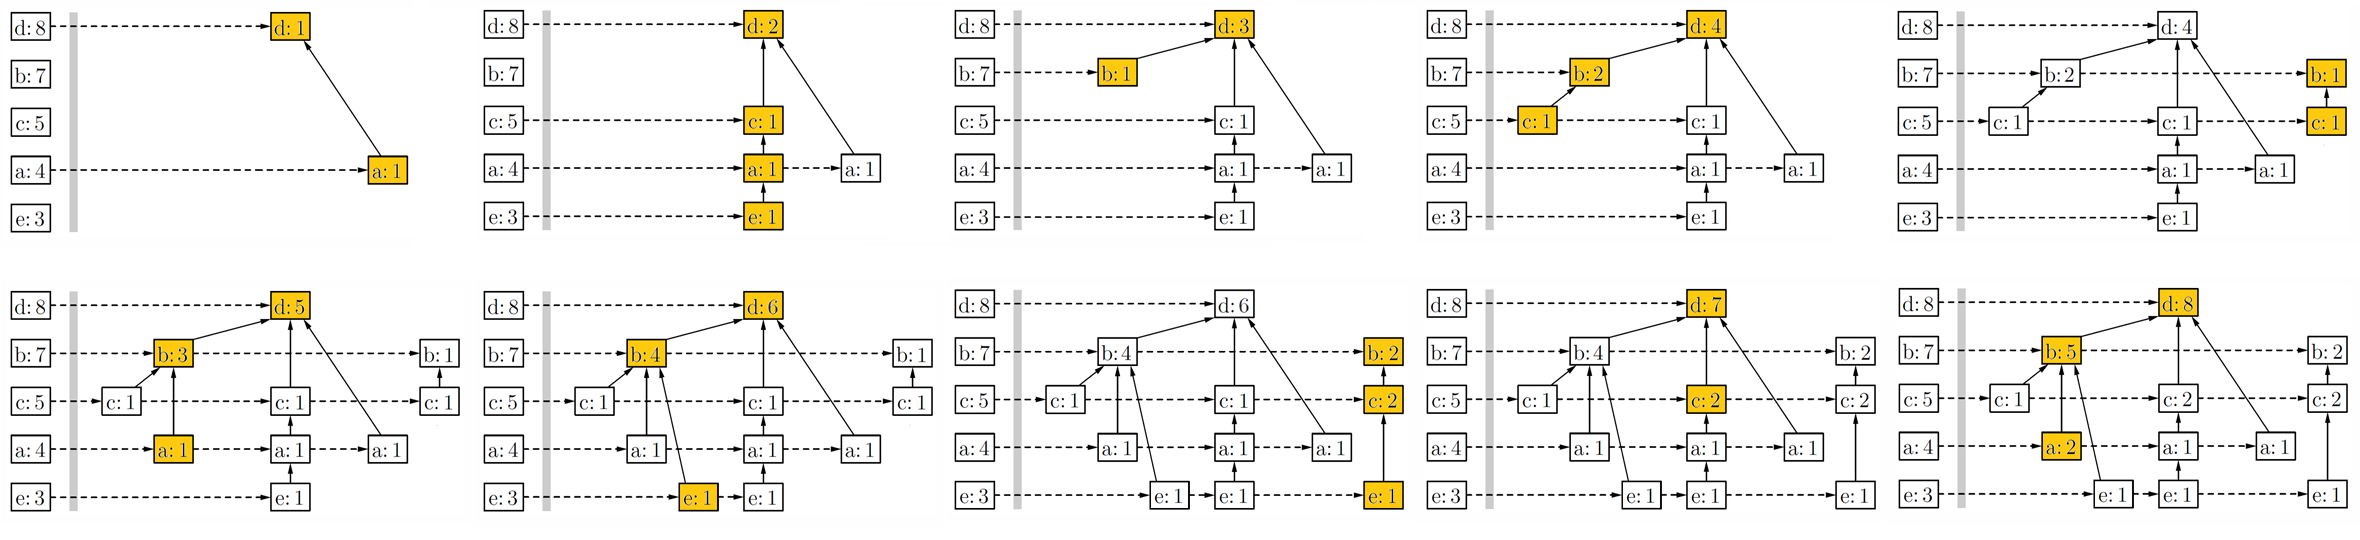
\includegraphics[width=1\linewidth]{chapters/metric/images/fp-tree-stages-example.png}
    \caption{Иллюстрация этапов построения FP-дерева}
    \label{fig:enter-label}
\end{figure}

\textbf{Введём обозначения:}

\begin{itemize}
    \item $V(T, f) = {v \in T: f_v = f}$ - все вершины, соответствующие признаку $f$. Соответственно, у них равные глубины.
    \item $C(T, f) = \displaystyle\sum_{v \in V(T, f)} c_v$ - Сумма счетчиков вершин, соответствующих признаку $f$. Несложно понять, что эта сумма равна числу объектов $x_i \in U$, для которых $f(x_i) = 1$. Другими словами $C(T, f) = l\nu(f)$
\end{itemize}


\subsection{Построение условного FP-дерева}

Прежде чем приступить к второму этапу алгоритма, разберёмся в одной важной для него процедуре. 
\newline\newline
\textbf{Определение.} Пусть FP-дерево $T$ построено по подвыборке $U$. Условное FP-дерево $T' = T|\varphi$ - это FP-дерево, порождаемое подвыборкой $\{x_i \in U| \varphi(x_i) = 1 \}$ из которого удалены все вершины признака $f$ и ниже.
\newline\newline
Рассмотрим алгоритм построения $T|f$ по $T$, где $f$ - признак из $\mathcal{F}$:
\begin{enumerate}
    \item Оставим в дереве только те вершины, которые принадлежат путям, идущим от вершин признака $f$ до корня. 
    \item Обновим счетчики $c_i$: для вершин признака $f$ ничего не меняем, а для остальных рекурсивно снизу вверх обновляем по формуле $c_u = \displaystyle\sum_{w \in S_u} c_w$
    \item Удаляем вершины признака $f$ из $T'$.
\end{enumerate}

Корректность следует из построения.

\subsection{Построение списка ассоциативных правил}

Для начала поймем, как эффективно находить $\nu(\varphi)$ используя FP-дерево. Для этого мы можем просто найти $f =argmin_{f \in \varphi} (\nu(f))$ и просуммировать $c_v$ для всех вершин $v$ признака $f$, таких что $\varphi \subset [f_{v_0}, f_{v}]$, где $[f_{v_0}, f_{v}]$ - набор признаков $f_{v_i}$ вершин из пути от корня до $v$.
\newline\newline
Рассмотрим функцию FP-find$(T,\varphi,R)$, которая находит по FP-дереву $T$, все частные наборы, содержащие только частный набор $\varphi$, и признаки, которые в FP-дереве стотят выше всех признаков из $\varphi$, и добавляет их в список $R$. Она играет ключевую роль в работе данного алгоритма. Вот как её можно реализовать:
\newline\newline
\textbf{Псевдокод:}

\noindent\hrulefill % Горизонтальная линия
\begin{enumerate}
    \item \textbf{ПРОЦЕДУРА} FP-find$(T,\varphi,R)$;
    \newline
    \quad \textit{Вход:} $T$ — FP-дерево, частный набор $\varphi$, список наборов $R$.
    \newline
    \quad \textit{Выход:} Добавить все частные наборы, содержащие $\varphi$ в $R$.
    \item \quad для всех $f \in \mathcal{F} : V(T,f) \neq \emptyset$ по уровням снизу вверх:
    \item \quad \quad если $C(T,f) \geq l\delta$ то:
    \item \quad \quad \quad набор $\varphi \cup \{f\}$ - частый, добавляем его в $R$;
    \item \quad \quad \quad $T':=T|f$ - условное FP-дерево;
    \item \quad \quad \quad FP-find$(T',\varphi \cup \{f\},R)$; - рекурсивно найти все частые наборы, содержащие $\varphi \cup \{f\}$
\end{enumerate}
\noindent\hrulefill % Горизонтальная линия
\newline\newline
Для получения списка всех частых наборов, мы можем просто запустить FP-find$(T,\emptyset,\emptyset)$. Алгоритм просмотрит все наборы в обратном лексикографическом порядке. Для выделения ассоциативных правил теперь можем запустить функцию AssocRules из алгоритма APriory.

\subsection{Задачи для практики}
\textbf{Задача 1.} Как используя FP-дерево, построенное по выборке $U$ найти а) самый частый набор, б) самый редкий набор?
\newline\newline
\textbf{Решение.} 
\newline
а) По свойству антимонотонности, один из наборов размера 1 будет самым часто встречаемым. Так как признаки в FP-дереве уже отсортированы по частоте, самым частым будет самый верхний. Сложность алгоритма получается равной $O(1)$.
\newline
б) Подмножество каждого пути из корня в FP-дереве соответствует какому-то набору. Также каждый набор, соответствующий строке в базе, соответствует какому-то пути в дереве. По свойству антимонотонности, одним из наборов, соответствующих путям из корня до листьев, должен быть самым редким. Количество упоминаний одного из таких наборов - это значение счетчика $c_v$ в соответствующем листе. То есть наша задача сводится к поиску листа с минимальным значением этого счетчика. Это можно сделать, пройдя обходом в глубину по всему дереву, за $O(2^n)$, где $n$ - глубина дерева в худшем случае.
\newline\newline
\textbf{Задача 2.} Как по уже построенному FP-дереву для выборки $U$ и фиксированных параметров поддержки $\delta$ и значимости $\chi$, найти все ассоциативные правила, удовлетворяющие $\delta, \chi$ вида $a \to b$, где $a,b \in \mathcal{F}$ за $O(n2^n)$ в худшем случае?
\newline\newline
\textbf{Решение.} 
\newline
Заметим, что всего таких правил порядка $n^2$, где $n$ - число признаков. То есть для того, чтобы дать ответ, нам достаточно найти $\nu(f), \nu(f \cup g)$ для всех признаков $f,g$ из дерева. Первые величины уже известны, так как были вычислены на первом этапе построения FP-дерева. Для нахождения всех $\nu(f \cup g)$, достаточно создать двумерный массив $C$, такой что $C_{fg}$ равно числу $x \in U: (f \wedge g)(x_i) = 1$. Для его заполнения мы можем пройти обходом в глубину по дереву, и находясь в вершине $v$, прибавлять $c_v$ к $C_{f_vf_u} = C_{f_uf_v}$ для всех $u \in [v_0, v]$, где $ [v_0, v]$ - путь от корня до $v$. Этот обход потребует порядка $O(n2^n)$ действий. То есть суммарно у нас уйдет $O(n2^n + n^2) = O(n2^n)$ действий.
\newline\newline
\textbf{Задача 3.}
Оцените время работы алгоритма FP-Growth для нахождения ассоциативных правил, удовлетворяющих поддержке $\delta$ и значимости $\chi$ в худшем случае.
\newline\newline
\textbf{Решение.} 
\newline
Если с временем построения FP-дерева все понятно - оно совпадает с временем построения бора по массиву строк и равно $O(nl)$. То асимптотика генерации всех частых наборов и выделение ассоциативных правил значительно труднее для вычисления. Построение условного FP-дерева $T|f$ по самому нижнему признаку $f$ выполняется одним обходом в глубину - асимптотически $O(2^n)$. Пусть FP-find$(T,\emptyset,\emptyset)$ выполняется за время $k(n)$, тогда $k(n) = O\left(\sum_{i = 0}^{n-1} (2^i + k(i))\right)$, где $2^i$ действий уходит на построение условного дерева по каждому из признаков. Сделаем замену $t(n):=2^n+k(n)$, тогда $t(n) - 2^n = O\left(\sum_{i = 0}^{n-1}t(i)\right)$, заметим, что для $t(n) = n2^n$ верно: $n2^n = O\left(\sum_{i = 0}^{n-1} i2^i\right) = O((n-2)2^n)$. Значит $k(n) = O(n2^n)$. Теперь найдем время выделения ассоциативных правил. Операция нахождения $\nu(\varphi)$ по данному $\varphi$ может быть оптимизирована с использованием дерева поиска для хранения множества $\varphi$, что даст суммарное время работы $O(nlogn + 2^d\cdot \log(n)) = O((2^d + n)\cdot \log(n))$, где $d$ - глубина самого нижнего признака из $\varphi$. Для выделение ассоциативных правил из набора $\varphi$ длинны $k$, время упирается в скорость вычисления $\nu(\varphi')$ для проверки $\nu(y' | \varphi') \geq \chi$, поэтому оно будет не хуже, чем $O(2^k \cdot (2^d + n)\cdot \log(n)))$, и не лучше $O(2^{k-1} \cdot (2^d + n)\cdot \log(n)))$ - так как есть $2^{k-1}$ набор содержащий признак глубины $d$, поддержку которого надо вычислить. Наконец выделение всех ассоциативных правил для всех частых наборов в худшем случае будет порядка 
$$O\left(\sum_{d = 1}^{n} \sum_{k = 1}^{n-d} \mathrm{C}_{n-d}^{k} \cdot 2^{k-d}\cdot \log(n) \right) =
O\left(\sum_{d = 1}^{n} \frac{3^{n-d}}{2^d} \cdot\log(n) \right) =O(3^n \log(n))  $$
Что и будет решающим слагаемым в асимптотике работы всего алгоритма.


\section{Алгоритм APriory}

\subsection{Свойство антимонотонности}
Алгоритм \textbf{APriory} основывается на свойстве \textbf{антимонотонности} функции \( \varphi(x)= \bigwedge_{f \in \varphi} f(x)\):

Для любых \( \psi, \varphi \subset \mathcal{F} \), из \( \varphi \subset \psi \) следует \( \nu(\varphi) \geq \nu(\psi) \).

\textbf{Следствия:}

\begin{enumerate}
    \item Если \( \psi \) частый, то все его подмножества \( \varphi \subset \psi \) частые.
    \item Если \( \varphi \) не частый, то все наборы \( \psi \supset \varphi \) также не частые.
    \item \( \nu(\varphi \cup \psi) \leq \nu(\varphi) \) для любых \( \varphi, \psi \).
\end{enumerate}

Основываясь на этих свойствах, мы можем построить итеративный алгоритм нахождения ассоциативных правил (\textbf{APriory}). Алгоритм состоит из двух этапов:

\begin{enumerate}
    \item Поиск частых наборов 
    \item Выделение ассоциативных правил
\end{enumerate}

Вторая часть алгоритма считается полностью \textit{решенной}, так как существует простая и эффективная процедура, реализующая её. Первая же часть представляет наибольший интерес, так как требует многократное обращение к базе данных, поэтому стоит важный вопрос оптимизации этого этапа.

\subsection{Поиск частых наборов}

\textbf{Идея алгоритма:} на \( j\) этапе храним все \textit{частые наборы} мощности \(j\): \(G_j\). Тогда при переходе от \(G_j\) к \(G_{j+1}\) пытаемся увеличить каждое из множеств \(\varphi \in G_j\), чтобы оно по-прежнему оставалось \textit{частым набором}.
\newline\newline
\textbf{Псевдокод:}
\newline
\textit{Вход:} \( X^\ell \) — обучающая выборка; минимальная поддержка \( \delta \); минимальная значимость \( \chi \).
\newline
\textit{Выход:} \( R = \{(\varphi, \psi)\} \) — список ассоциативных правил.

\noindent\hrulefill % Горизонтальная линия
\begin{enumerate}
    \item Множество \textbf{всех частых} исходных признаков: \newline
    \(G_1 := \{ f \in \mathcal{F} \mid \nu(f) \geq \delta \};\)
    
    \item \textbf{Для всех} \( j = 2, \ldots, n \):
     \item \quad Множество \textbf{всех частых} наборов мощности \( j \): 
     \[
     G_j := \{ \varphi \cup \{f\} \mid \varphi \in G_{j-1}, \, f \in G_1, \, \nu(\varphi \cup \{f\}) \geq \delta \};
    \] 
        \item \quad \textbf{Если} \( G_j = \emptyset \), то:
            \item \quad  \quad\textbf{выход} из цикла по \( j \);
    \item \( R := \emptyset \);
    \item \textbf{Для всех} \( \psi \in G_j, \, j = 2, \ldots, n \):
    \item \quad \texttt{AssocRules}( \( R, \psi, \emptyset \) );
\end{enumerate}
\noindent\hrulefill % Горизонтальная линия
\newline

Заметим, что за лаконичной математической формулой \(\nu(\varphi \cup \{f\}) \geq \delta \) на самом деле скрывается просмотр базы данных, что делает эту проверку очень тяжелой. 

\subsection{Выделение ассоциативных правил.}
\textbf{Идея алгоритма:} \textit{отщипываем} по одному признаку из \(\varphi\), проверяем ассоциативность получившегося правила.
\newline\newline
\textbf{Псевдокод:}
\newline
\textit{Вход:} $R$ — список ассоциативных правил; \\
\textit{Выход:} $(\varphi, y)$ — ассоциативное правило;

\noindent\hrulefill % Горизонтальная линия
\begin{enumerate}
    \item \textbf{ПРОЦЕДУРА} AssocRules $(R, \varphi, y)$;
    \item \quad \textbf{для всех} $f \in \varphi$
    \item \quad \quad $\varphi' := \varphi \setminus \{f\}$; \quad $y' := y \cup \{f\}$;
    \item \quad \quad \textbf{если} $\nu(y' | \varphi') \geq \chi$ \textbf{то}
    \item \quad \quad \quad добавить ассоциативное правило $(\varphi', y')$ в список $R$;
    \item \quad \quad \textbf{если} $|\varphi'| > 1$ \textbf{то}
    \item \quad \quad \quad AssocRules $(\varphi', y')$;
\end{enumerate}
\noindent\hrulefill % Горизонтальная линия
\newline
\subsection{Задачи для практики}

\subsubsection{Задача 1: Простота алгоритма APriory:} Чтобы лучше прочувствовать алгоритм APriory (а также убедиться в его простоте) проделайте его руками для следующей таблицы транзакций (числа - номера транзакции, буквы - признаки), а именно найдите все частые наборы признаков (\(G_1, G_2, \ldots)\)) при \( \text{minsup}=0.3 \).
\begin{table}[h!]
\centering
\caption{Таблица транзакций}
\begin{tabular}{ccccccc}
\toprule
\textbf{Транзакция} & \textbf{A} & \textbf{B} & \textbf{C} & \textbf{D} & \textbf{E} & \textbf{F} \\
\midrule
1  & 1 & 1 & 1 & 0 & 0 & 0 \\
2  & 1 & 0 & 1 & 1 & 0 & 0 \\
3  & 0 & 1 & 1 & 1 & 1 & 0 \\
4  & 1 & 1 & 0 & 1 & 0 & 1 \\
5  & 1 & 0 & 1 & 1 & 1 & 0 \\
6  & 0 & 1 & 1 & 0 & 0 & 0 \\
7  & 1 & 1 & 1 & 0 & 1 & 0 \\
8  & 1 & 0 & 0 & 1 & 1 & 1 \\
9  & 0 & 1 & 1 & 1 & 0 & 0 \\
10 & 1 & 1 & 1 & 0 & 1 & 0 \\
\bottomrule
\end{tabular}
\end{table}
\newline
\textit{Решение:}

\textbf{Шаг 1: Частые одноэлементные наборы (\( G_1 \))}

Считаем поддержку для каждого элемента:
\[
\begin{aligned}
&\{A\}: 7, \quad \{B\}: 6, \quad \{C\}: 8, \quad \{D\}: 6, \quad \{E\}: 5, \quad \{F\}: 2.
\end{aligned}
\]

Частые одноэлементные наборы (\( support \geq 3 \)):

\[
G_1 = \{\{A\}, \{B\}, \{C\}, \{D\}, \{E\}\}.
\]

\textbf{Шаг 2: Частые пары (\( G_2 \))}

Формируем все возможные пары элементов (\( \varphi_2 \)) и считаем их поддержку:

\[
\begin{aligned}
&\{A, B\}: 4, \quad \{A, C\}: 4, \quad \{A, D\}: 4, \quad \{A, E\}: 4, \\
&\{B, C\}: 6, \quad \{B, D\}: 3, \quad \{B, E\}: 3, \\
&\{C, D\}: 4, \quad \{C, E\}: 4, \quad \{D, E\}: 3.
\end{aligned}
\]

Частые пары (\( support \geq 3 \)):

\[
G_2 = \{\{A, B\}, \{A, C\}, \{A, D\}, \{A, E\}, \{B, C\}, \{B, D\}, \{B, E\}, \{C, D\}, \{C, E\}, \{D, E\}\}.
\]

\textbf{Шаг 3: Частые тройки (\( G_3 \))}

Формируем тройки (\( \varphi_3 \)) и считаем их поддержку:

\[
\begin{aligned}
&\{A, B, C\}: 3, \quad \{A, B, D\}: 1, \quad \{A, B, E\}: 1, \\
&\{A, C, D\}: 2, \quad \{A, C, E\}: 3, \quad \{A, D, E\}: 1, \\
&\{B, C, D\}: 2, \quad \{B, C, E\}: 3, \quad \{B, D, E\}: 1, \\
&\{C, D, E\}: 1.
\end{aligned}
\]

Частые тройки (\( support \geq 3 \)):

\[
G_3 = \{\{A, B, C\}, \{A, C, E\}, \{B, C, E\}\}.
\]

\textbf{Шаг 4: Частые четверки (\( G_4 \))}

Формируем четверки (\( \varphi_4 \)):

\[
\{A, B, C, E\}: 1.
\]

Поддержка меньше минимальной (\( support < 3 \)), поэтому завершаем алгоритм.

\subsubsection{Задача 2: Сложность алгоритма APriory:} К.В. Воронцов так отзывался об алгоритме APriory: "Простой, классический, везде описанный, но пользоваться им не надо". Мы уже упоминали о неэффективности этого алгоритма, теперь убедитесь в этом сами: посчитайте временную асимптотику и асимптотику используемой памяти (обозначим \(|D|\) - количество признаков)


\textit{Решение:} Если размер максимального по включению частого множества \(|S|\), то мы переберем также все его подмножества, то есть пройдет \(\mathcal{O}(2^{|S|})\) итераций. Итого асимптотика \(\mathcal{O}(2^{|D|})\)

Пусть снова \(S\) - максимальное частое множество. Значит все его подмножества - также частые множества, значит они также будут сохранены, значит памяти будет занято \(\mathcal{O}(2^{|S|})\). Итоговая асимптотика памяти \(\mathcal{O}(2^{|D|})\).

Основная проблема алгоритма - мы наивно ищем частые наборы. Следующий алгоритм \textit{FP-Growth} признан решить эту проблему, используя эффективные структуры данных для быстрого поиска.

\subsubsection{Задача 3: Недостатки алгоритма APriory на практике:} В прошлой задаче мы убедились в неэффективности алгоритма с точки зрения его временной сложности. Подумайте теперь о недостатках алгоритма при его использовании на практике (не считая временной сложности). Для ответа вспомните примеры использования ассоциативных правил в жизни.

\textit{Решение:} Вспомнил классический пример применения поиска ассоциативных правил — анализ рыночной корзины. При непосредственном использовании алгоритма, где товары рассматриваются как признаки, а чеки — как объекты, возникает важная проблема: нам необходимо не просто анализировать отдельные товары, а учитывать сгруппированные категории. Например, нас интересует не просто покупка конкретных видов хлеба, а сам факт приобретения хлебобулочных изделий (или, например, приобретения черного хлеба). Таким образом, нужно учитывать иерархию признаков.

Другая проблема - мы никак не учитываем информацию о самих клиентах (например, семейное положение, возраст\(\ldots\)). На практике при построении ассоциативных правил эта информация сильно влияет на правила, поэтому их нельзя игнорировать.

\section{Задача автоматического выделения терминов: алгоритм TopMine, UDPipe, модель PLSA.}

Цель для такой задачи является выделение составных терминов в текстовых коллекциях. Термин - фраза (n-грамма) со следующим набором свойств:

\begin{itemize}
	\item Высокая частотность - много раз встречается в коллекции.
	\item Контактная сочетаемость слов - состоит из слов, неслучайно часто встречающихся вместе.
	\item Полнота - является максимальной по включению цепочкой слов.
	\item Синтактическая свяхность - является грамматически корректным словосочетанием.
	\item Тематичность - часто встречается в узком подмножестве тем.
\end{itemize}

Для проверки каждой из свойств используются 

\begin{itemize}
	\item Статистический анализ: для проверки первых трёх свойств терминов. Он позваляет находить высокочастотные токены, выделять слова, неслучайно стоящие рядом и штрафовать неполные последовательности слов, входящие как подмножество в другую высокочастотную последовательность неслучайно стоящих слов.
	\item Синтаксический анализ: для проверки синтактической связности. Данный анализ позволяет выделять синтактически связанные словосочетания в предложениях.
	\item Тематическая модель: для проверки тематичности. Она позволяет сопоставить каждому токену распределение тем.
\end{itemize}

Для каждого анализа мы будем использовать модели TopMine, UDPipe и PLSA для семантического, синтаксического анализа и тематической модели соответственно. Рассмотрим в подробности каждую модель

\subsection*{Статистический анализ: TopMine}

Этот алгоритм итеративно сливает слова и фразы в предложении, рассчитывая для каждого слияния оценку значимости \textit{SignificanceScore} и останавливается, когда для всех возможных слияний значимость меньше заданного порога. 

В начале мы должны найти все частые k-грамм и алгоритм быстрого поиска приведён на рисунке 1.
\begin{figure}
    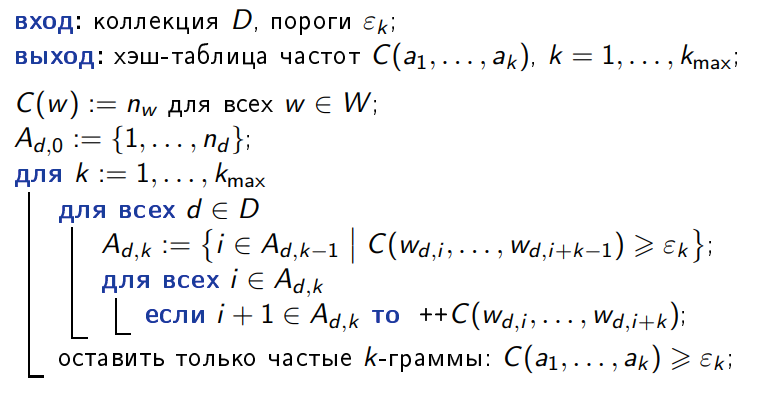
\includegraphics[scale = 0.5]{images/ml1.png}
    \caption{Алгоритм быстрого поиска}
\end{figure}
где $C(a_{1},...,a_{k})$ - хэш-таблица частот k-грамм, $a_{i} \in W$, $C(w) = n_{w}$ для всех униграмм $w \in W: n_{w} \geq \varepsilon_{1}$, где $W$ - множество слов или фраз.
$\varepsilon_{1}$ - пороговое значение частоты частых k-грамм
$A_{d,k}$ - множество позиций i в документе d, с которых начинаются все частые k-граммы
$C(w_{d,i},...,w_{d,i+k-1}) \geq \varepsilon_{k}$
Свойство антимонотонности: $C(a_{1},...,a_{k}) \geq C(a_{1},...,a{k+1})$

Затем должны провести итеративное слияние фраз с понижением значимости до $\alpha$.
$SignificanceScore = \frac{p_{uv}-p_{u}p_{v}}{\sqrt{p_{uv}}}$
где $p_{u}$ - оценка вероятности встретить фразу \textit{u}, $p_{uv}$ = оценка вероятности встретить фразу \textit{uv}.

В начале у нас есть кортеж исходных фраз и первой итерацией считается \textit{SignificanceScore} для всех соседних пар фраз. И затем из кортежа удаляются все все пары с \textit{SignificanceScore} больше $\alpha$. Оставшиеся элементы в кортеже и являются термами. На рисунке 2 приведен пример работы алгоритма TopMine.
\begin{figure}
    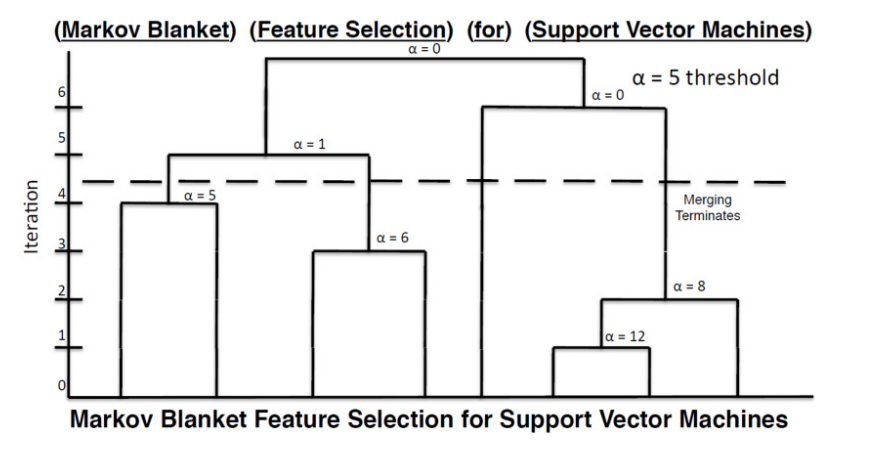
\includegraphics[scale = 0.5]{images/ml2.png}
    \caption{Пример работы алгоритма TopMine}
\end{figure}
\subsection*{Синтаксический анализ: UDPipe}

UDPipe - предобученная модель, которая может распозновать синтаксические связи в предложениях и разметка частей речи слов в предложениях. На вход подаётся список предложений, и для каждого слова в предложениях вычисляется:

\begin{itemize}
	\item Часть речи слова.
	\item Член предложения.
	\item ID родительского слова.
\end{itemize}

Модель для каждого предложения создаёт синтаксическое дерево, и при помощи неё проверяет словосочетании-кандидаты. Для них подсчитывается оценка его синтаксической связанности по формуле $SyntaxScore(W) = max SyntaxDistance(w_{i}, w_{j})$, где \textit{W} - N-грамма, $1 \leq i \leq N$, $1 \leq j \leq N$ и $i \neq j$.Таким образом, если одно из слов в словосочетании-кандидате синтактически не связанно с остальным, \textit{SyntaxScore} это выявит.

\subsection*{Тематический анализ: PLSA}

У нас есть коллекция текстовых документов $D$ и словарь токенов $W$, из которых состоят документы. Каждый документ $d \in D$ представляет собой последовательностью входящих в него токенов из словаря $W$. Если предположить, что местоположение токенов в документе не влияет на определение тематики документа, то документ это подмножество $d \subset W$, в котором каждому токену $w \in d$ поставлено в соответствие число $n_{dw}$ вхождений в документ $d$.

Модель описывает вероятности появления токенов $w$ в документов $d$ при предположении условной независимости:
$$p(w|d) = \sum_{t \in T} p(w|t)p(t|d) = \sum_{t \in T} \phi_{wt} \theta_{td}$$
где $\phi_{wt} = p(w|t), \theta_{td} = p(t|d)$ являются обучаемыми параметрами модели. Для обучения параметров модели, представленные в виде матрицы $\Phi = (\phi_{wt})_{WxT}$ и $\Theta = (\theta_{td})_{TxD}$ по коллекции документов $D$ максимизируется логарифм правдоподобия
$$L(\Phi, \Theta) = \sum_{d \in D} \sum_{w \in d} n_{dw} ln \sum_{t \in T} \phi_{wt} \theta_{td} \rightarrow \max_{\Phi, \Theta}$$

при ограничениях неотрицательности и нормировки
$$\sum_{w \in W} \phi_{wt} = 1, \phi_wt \geq 0, \sum_{t \in T} \theta_{td} = 1, \theta_{td} \geq 0$$

На основе полученных параметров $\Phi$ и $\Theta$ для каждого словосочетания-кандидата считается распределение тем $p(t|w) = \phi_{wt} \frac{p(t)}{p(w)}$. Отбор происходит распределением тематик $p(t|w)$ имеет высокую вероятность только для некоторых тем из малого подмножества всех тем T. Это можно оценить через отдаленность $p = p(t|w)$ от равномерного $p_{unif} = 1/T$, где $T$-мощьность множества $T$. Расстояние между двумя распределениями считается несколькими способами:

\begin{itemize}
	\item Дивергенция Кульбака-Лейблера
	$$KL(pp_{unif}) = \sum_{t \in T} \frac{1}{|T|} ln \frac{\frac{1}{|T|}}{p(t|w)}$$
	\item Дивергенция Йесена-Шеннона
	$$JS(pp_{unif}) = \frac{1}{2}KL(p_{unif}p_{1}) + \frac{1}{2}KL(pp_{1})$$
	$$p_{1}(t|w) = \frac{1}{2}(p(t|w) + \frac{1}{|T|})$$
	\item Сумма степенных функций, $\gamma > 1$
	$$Deg(p) = \sum_{t \in T} p(t|w)^{\gamma}$$
\end{itemize}

Чем больше значение данных метрик для $w$, тем тематичнее данная N-грамма.

\subsection*{Задачи}

\textbf{Задача 1.} Нам дана фраза \textit{a} \textit{b}, было оценено вероятность встречи фраз $p_{a} = 0,1$, $p_{b} = 0,2$, $p_{ab} = 0,05$. Пороговая значимость $\alpha = 1$. Является ли фраза \textit{ab} термином?

\textbf{Ответ:} Нет.

\textbf{Решение.} 
$$\frac{p_{ab}-p_{a}p_{b}}{\sqrt{p_{ab}}} \approx 0,01 < \alpha$$

 \textbf{Задача 2.} Дано синтактическое дерево (рис. 3) для предложения "An inventory of syntactic functions is taken to be primitive". Найдите \textit{SyntaxScore} для фразы "syntactic functions is".
 
\begin{figure}
    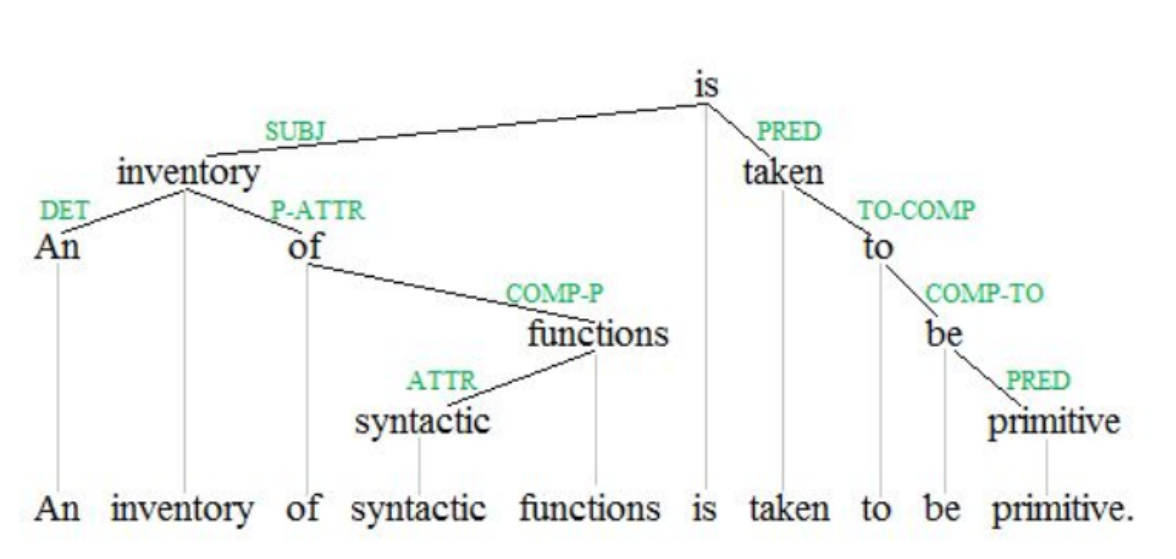
\includegraphics[scale = 0.4]{images/ml3.png}
    \caption{Задача 2}
\end{figure}

\textbf{Ответ:} 4.

\textbf{Задача 3.} Привести аналитическое решение максимизации задачи

$$L(\Phi, \Theta) = \sum_{d \in D} \sum_{w \in d} n_{dw} ln \sum_{t \in T} \phi_{wt} \theta_{td} \rightarrow \max_{\Phi, \Theta}$$

и выразить элементы матрицы $\Phi$ и $\Theta$ через $n_{dw}$ и $p(t|d,w)$.

\textbf{Решение.}

Запишем лангранжиан задачи, учитывая ограничение нормировки:

$$L(\Phi, \Theta) = \sum_{d \in D} \sum_{w \in d} n_{dw} ln \sum_{t \in T} \phi_{wt} \theta_{td} - \sum_{t \in T} \lambda_{t} (\sum_{w \in d} \phi_{wt} - 1) - \sum_{d \in D} \mu_{d} (\sum_{t \in T} \theta_{td} - 1)$$

Продифференцируем лангранжиан по $\phi_{wt}$ и приравняем к нулю производную, получим:

$$\lambda_{t} = \sum_{d \in D} n_{ds} \frac{\theta_{td}}{p(w|d)}$$

Домножив обе части на $\phi_{wt}$, получим:

$$\lambda_{t} \phi_{wt} = \sum_{d \in D} n_{ds} \frac{\phi_{wt} \theta_{td}}{p(w|d)}$$

По формуле Байеса:

$$p(t|d,w) = \frac{p(w|t) p(t|d)}{p(w|d)} = \frac{\phi_{wt} \theta_{td}}{p(w|d)}$$

Сделав замену  получим:

$$\lambda_{t} \phi_{wt} = \sum_{d \in D} n_{ds} p(t|d,w)$$

Просуммируем по $w \in W$ и получим:

$$\lambda_{t} \sum_{w \in W} \phi_{wt} = \sum_{w \in W} \sum_{d \in D} n_{ds} p(t|d,w)$$

В соответствии с условием нормировки $\sum_{w \in W} \phi_{wt} = 1$:

$$\lambda_{t} = \sum_{w \in W} \sum_{d \in D} n_{ds} p(t|d,w)$$

Выразив из $\lambda_t \phi_{wt} = \sum_{d \in D} n_{dw} p(t|d,w)$ $\phi_{wt}$ и подставив $\lambda_{t}$ получаем:

$$\phi_{wt} = \frac{\sum_{d \in D} n_{dw} p(t|d,w)}{\sum_{w_{1} \in W} \sum_{d \in D} n_{dw_{1}} p(t|d,w_{1})}$$

Для $\theta_td$ поступаем аналогично. После приравнивания производной по $\theta_{td}$ к $0$, домнажения на $\theta_{td}$, суммирования по всем $t \in T$ находим $\mu_{d}$:

$$\mu_{d} = \sum_{t \in T} \sum_{w \in d} n_{dw} p(t|d,w)$$

Выразим $\theta_{td}$:

$$\theta_{td} = \frac{\sum_{w \in d} n_{dw} p(t|d,w)}{\sum_{w \in d} n_{dw} \sum_{t_{1} \in T} p(t_{1}|d,w)}$$


\section{\textbf{\textit{ECLAT (Equivalence Class Transformation) алгоритм}}}
\textbf{\textit{Prerequisites:}} Задача поиска ассоциативных правил: определения/прикладные задачи/связь с логическими закономерностями, \textit{Apriori} алгоритм.\newline\newline
\textit{ECLAT} — это эффективный алгоритм для поиска частых наборов элементов с использованием вертикального представления данных. Его основная идея заключается в том, чтобы представлять данные в виде списка идентификаторов транзакций (\textit{TID, Transaction IDs}) для каждого элемента и находить частые наборы через пересечение этих списков.

\subsection{\textbf{Основные шаги работы алгоритма}}
\begin{enumerate}
    \item {\textbf{\textit{Представление данных}}:\newline
   Данные представляются в вертикальном виде: для каждого элемента (\(A\)) создается список транзакций (\(TID\)), где этот элемент встречается.\newline
   Пример:\par  
     Данные в транзакционном виде:  
     \[
     \text{T1: A, B, C}, \quad \text{T2: A, C}, \quad \text{T3: A, B}, \quad \text{T4: B, C}.
     \]  \par
     Вертикальное представление:  
     \[
     A: \{1, 2, 3\}, \quad B: \{1, 3, 4\}, \quad C: \{1, 2, 4\}.
     \]}
     \item {\textbf{\textit{Пересечение списков}}:\newline
   Для каждого кандидата (например, \(AB\)) пересекаются списки транзакций:  
     \[
     AB = A \cap B = \{1, 3\}.
     \]\newline
   Если размер пересечения (\(support\)) больше порога (\(min\_support\)), набор считается частым.}
   \item {\textbf{\textit{Рекурсия}}:\newline
   Наборы элементов увеличиваются итеративно, добавляя новые элементы и проверяя пересечения списков \(TID\).}
   \item {\textbf{\textit{Вывод частых наборов}}:\newline
   В результате сохраняются все наборы, частота которых превышает заданный порог.}
\end{enumerate}

\subsection{\textbf{Преимущества и недостатки ECLAT по сравнению с Apriori}}
  ECLAT алгоритм обладает рядом преимуществ и особенностей по сравнению с алгоритмом Apriori:
  \begin{enumerate}
      \item {\textbf{\textit{Структура данных}}:\newline
      Eclat использует подход поиска в глубину и классы эквивалентности для сокращения пространства поиска.\newline
      Apriori использует поиск в ширину и генерацию кандидатов, что может быть затратным с точки зрения вычислений.}
      \item {\textbf{\textit{Масштабируемость}}:\newline
      Eclat часто более эффективен в плане памяти, чем Apriori, поскольку ему не нужно явно генерировать наборы элементов-кандидатов. Apriori может страдать от генерации большого количества кандидатов, особенно при работе с наборами данных с большим количеством элементов.}
      \item {\textbf{\textit{Сложность алгоритма}}:\newline
      Eclat, как правило, быстрее Apriori на практике для плотных наборов данных с низкими минимальными порогами поддержки. Производительность Apriori может ухудшаться, когда минимальная поддержка низкая, поскольку он генерирует много наборов элементов-кандидатов.}
      \item {\textbf{\textit{Распараллеливание}}:\newline
      Eclat легче распараллелить из-за его природы поиска в глубину. Подход Apriori в ширину менее естественно параллелизуем.}
  \end{enumerate}
  Среди недостатков можно выделить следующие:
  \begin{enumerate}
      \item {Требует много памяти для хранения вертикального представления.}
      \item {Может быть неэффективным для разреженных данных.}
  \end{enumerate}
\subsection{Общие выводы}
Подводя итог, можно сказать, что алгоритм \textit{Eclat} — это метод глубинного частого поиска элементов, который использует классы эквивалентности для эффективного поиска шаблонов в транзакционных наборах данных. Он имеет некоторые преимущества перед алгоритмом \textit{Apriori}, особенно с точки зрения эффективности памяти и масштабируемости, что делает его ценным инструментом для поиска правил ассоциации.

\subsection{Теоретические задачи и их решения}
\bigskip
\begin{enumerate}
    \item {\textbf{Найти частые наборы элементов с \(min\_support = 2\).}\newline
    
    1. \textit{Шаг 1. Одинарные элементы:}\par
       - \(A: \{1, 2, 3\}\), \(B: \{1, 3, 4\}\), \(C: \{1, 2, 4\}\).\newline
       - Частота: \(A = 3\), \(B = 3\), \(C = 3\). Все частые.\newline
    2. \textit{Шаг 2. Двойные наборы (пересечения):}\par
       - \(AB = A \cap B = \{1, 3\}\), частота = 2.\newline
       - \(AC = A \cap C = \{1, 2\}\), частота = 2.\newline
       - \(BC = B \cap C = \{1, 4\}\), частота = 2.\newline
       Все частые.\newline
    3. \textit{Шаг 3. Тройные наборы (пересечения):}\par
       - \(ABC = A \cap B \cap C = \{1\}\), частота = 1. Не частый.\newline    
    \textbf{\textit{Результат:}}
    \[
    \text{Частые наборы: } \{A\}, \{B\}, \{C\}, \{AB\}, \{AC\}, \{BC\}.
    \]}
    \item {\textbf{Построить ассоциативные правила с \(min\_confidence = 50\%\).}\newline
    \textit{Данные частотности:}\newline
    \(A: 3\), \(B: 3\), \(C: 3\), \(AB: 2\), \(AC: 2\), \(BC: 2\).
    
    \textit{Шаги для генерации правил:}\newline
    1. Для \(AB\):\par 
       \(A \rightarrow B: \text{Confidence} = \frac{\text{Support}(AB)}{\text{Support}(A)} = \frac{2}{3} \approx 66.7\%\).  
         Правило проходит.\newline 
       \(B \rightarrow A: \text{Confidence} = \frac{\text{Support}(AB)}{\text{Support}(B)} = \frac{2}{3} \approx 66.7\%\).  
         Правило проходит.\newline
    2. Для \(AC\):\par  
       \(A \rightarrow C: \text{Confidence} = \frac{\text{Support}(AC)}{\text{Support}(A)} = \frac{2}{3} \approx 66.7\%\).  
         Правило проходит. \newline 
       \(C \rightarrow A: \text{Confidence} = \frac{\text{Support}(AC)}{\text{Support}(C)} = \frac{2}{3} \approx 66.7\%\).  
         Правило проходит.\newline
    3. Для \(BC\):\par
       Аналогично, \(B \rightarrow C\) и \(C \rightarrow B\) проходят.\newline
    
    \textbf{\textit{Результат:}}\newline
    \[
    \text{Ассоциативные правила: } A \rightarrow B, B \rightarrow A, A \rightarrow C, C \rightarrow A, B \rightarrow C, C \rightarrow B.
    \]}
    \item {\textbf{Оценить производительность ECLAT при увеличении числа элементов.}:\newline
    Предположим:\par
    \(N\) — количество транзакций.\newline
    \(M\) — количество элементов.\newline
    \textbf{\textit{Вопрос}}: Как изменится производительность ECLAT, если \(M\) увеличится вдвое?\newline
    \textbf{\textit{Решение:}}\newline 
    1. В вертикальном представлении для каждого элемента требуется хранить его список \(TID\) $\Rightarrow$ при увеличении \(M\) вдвое потребуется в 2 раза больше памяти.\newline
    2. Число возможных пересечений растёт экспоненциально $\Rightarrow$ если ранее было \(2^M - 1\) наборов, то теперь будет \(2^{2M} - 1\).\newline
    3. Производительность ухудшится, так как пересечение бОльших списков потребует больше времени.\newline}
\end{enumerate}
Эти задачи показывают применение ECLAT в поиске частых наборов, генерации ассоциативных правил и анализе сложности алгоритма.


    \clearpage
    \chapter{Композиции классификаторов}
    \section{Mixture of Experts (Смесь экспертов)}

Модель \textit{Смеси экспертов} (Квазилинейный ансамбль, Mixture of Experts, MoE) является архитектурой машинного обучения, которая сочетает в себе несколько моделей (экспертов) для решения сложных задач. Основная идея заключается в том, чтобы разделить пространство входных данных на части, в каждом из которых определенный эксперт специализируется. Общая модель обучается так, чтобы комбинировать выходы экспертов с учетом их специализации.

Математически, выход модели MoE для признакового описания объекта $\mathbf{x}$ может быть представлен как:

$$
y = \sum_{k=1}^{K} g_k(\mathbf{x}) f_k(\mathbf{x}),
$$

где:
\begin{itemize}
    \item $K$ — количество экспертов,
    \item $f_k(\mathbf{x})$ — локальная модель, функция $k$-го эксперта, производящая прогноз,
    \item $g_k(\mathbf{x})$ — шлюзовая функция или функция компетентности, определяющая вес вклада $k$-го эксперта, причём $\sum_{k=1}^{K} g_k(\mathbf{x}) = 1$ и $g_k(\mathbf{x}) \geq 0$ для всех $k$.
\end{itemize}

Шлюзовая (Gate) функция обычно моделируется с помощью функции softmax

$$
g_k(\mathbf{x}) = \frac{\exp(h_k(\mathbf{x}))}{\sum_{j=1}^{K} \exp(h_j(\mathbf{x}))},
$$

где $h_k(\mathbf{x})$ — функция компетентности для $k$-го эксперта. Выбираются из каких-либо содержательных соображений.

Преимущество MoE заключается в способности моделировать сложные зависимости путем разделения задачи между специализированными экспертами, что может улучшить обобщающую способность и эффективность обучения.

\subsection{Задачи и решения}

\subsubsection{Задача 1}

Пусть имеется модель MoE с двумя экспертами, функции которых заданы как $f_1(x) = 2x$ и $f_2(x) = x^2$. Функции $h_k (x):$ $h_1 (x) = -x$, $h_2 (x) = x$.

Требуется найти выражение для общего выхода модели $y$ в зависимости от $x$.

\textbf{Решение:}

Шлюзовая функция моделируется как:

$$
g_1(x) = \frac{\exp(-x)}{\exp(-x) + \exp(x)}, \quad g_2(x) = \frac{\exp(x)}{\exp(-x) + \exp(x)}.
$$

Суммарный выход модели:

$$
y = g_1(x) f_1(x) + g_2(x) f_2(x) = g_1(x) \cdot 2x + g_2(x) \cdot x^2.
$$

Подставим выражения для $g_1(x)$ и $g_2(x)$:

$$
y = \frac{\exp(-x)}{\exp(-x) + \exp(x)} \cdot 2x + \frac{\exp(x)}{\exp(-x) + \exp(x)} \cdot x^2.
$$

Поэтому итоговое выражение для $y$:

$$
y = \frac{\exp(-x) \cdot 2x + \exp(x) \cdot x^2}{\exp(-x) + \exp(x)}.
$$

\subsubsection{Задача 2}

Рассмотрим модель MoE, где шлюзовая функция выбирает только одного эксперта в зависимости от знака $x$:
$$
g_1(x) = 
\begin{cases} 
1, & \text{если } x \geq 0, \\ 
0, & \text{если } x < 0,
\end{cases}
$$
$$
g_2(x) = 
\begin{cases} 
0, & \text{если } x \geq 0, \\ 
1, & \text{если } x < 0.
\end{cases}
$$
Функции экспертов заданы как $f_1(x) = x^2$ и $f_2(x) = -x$. Найдите общий выход модели $y$ для любого $x$.

\textbf{Решение:}

Поскольку в каждый момент времени активен только один эксперт, общий выход модели определяется функцией активного эксперта.

Для $x \geq 0$: 
$$
g_1(x) = 1, \quad g_2(x) = 0, \quad y = g_1(x) f_1(x) = x^2.
$$

Для $x < 0$: 
$$
g_1(x) = 0, \quad g_2(x) = 1, \quad y = g_2(x) f_2(x) = -x.
$$

Таким образом, общий выход модели равен:
$$
y = 
\begin{cases} 
x^2, & \text{если } x \geq 0, \\ 
-x, & \text{если } x < 0.
\end{cases}
$$
Это означает, что модель ведет себя по-разному на положительных и отрицательных значениях $x$, отражая специализацию экспертов на разных областях входных данных.

\subsubsection{Задача 3}

Рассмотрим модель Mixture of Experts, состоящую из двух экспертных моделей $f_1$ и $f_2$, а также шлюзовой функции $g$. Пусть на вход подаётся одно признаковое значение $x$. Выражения для выходов моделей заданы следующим образом:

$$
f_1(x) = w_1 x + b_1, \quad f_2(x) = w_2 x + b_2, \quad g(x) = \sigma(v x + c)
$$

где $\sigma(z) = \frac{1}{1 + e^{-z}}$ — сигмоидальная функция активации, а $w_1, w_2, b_1, b_2, v, c$ — параметры модели.

Выход всей модели MoE определяется как:

$$
y(x) = g(x) f_1(x) + (1 - g(x)) f_2(x)
$$

\textbf{Вопрос:} Предположим, что при $x = 0$ мы наблюдаем, что $y(0) = 1$, $f_1(0) = 1$, $f_2(0) = 3$. Найдите значение $g(0)$.

\textbf{Решение:}

Из условия задачи при $x = 0$ имеем:

$$
y(0) = g(0) \cdot f_1(0) + (1 - g(0)) \cdot f_2(0) = g(0) \cdot 1 + (1 - g(0)) \cdot 3
$$

Подставляем известное значение $y(0) = 1$:

$$
g(0) \cdot 1 + (1 - g(0)) \cdot 3 = 1
$$
$$
g(0) + 3 - 3g(0) = 1
$$
$$
-2g(0) + 3 = 1
$$
$$
-2g(0) = -2
$$
$$
g(0) = 1
$$

Таким образом, $g(0) = 1$.


    \clearpage
    \chapter{Ансамблирования классификаторов}
    \documentclass[10pt,a4paper]{article}

\bibliographystyle{gost} 
\usepackage{cmap}
\usepackage[T2A]{fontenc}
\usepackage[utf8]{inputenc}
\usepackage[english,russian]{babel}
\usepackage{indentfirst}
\usepackage{amsmath}
\usepackage{bm}
\usepackage{graphicx}
\usepackage{verbatim}
\usepackage{authblk}
% Переопределение для удаления слова "and" перед последним автором
\renewcommand\Authands{, } % Удаляем слово "and"


\newcommand{\appropto}{\mathrel{\vcenter{
  \offinterlineskip\halign{\hfil$##$\cr
    \propto\cr\noalign{\kern2pt}\sim\cr\noalign{\kern-2pt}}}}}

\def\app#1#2{%
  \mathrel{%
    \setbox0=\hbox{$#1\sim$}%
    \setbox2=\hbox{%
      \rlap{\hbox{$#1\propto$}}%
      \lower1.1\ht0\box0%
    }%
    \raise0.25\ht2\box2%
  }%
}
\def\approxprop{\mathpalette\app\relax}


%%% Работа с русским языком
\usepackage{cmap}			 % поиск в PDF
\usepackage{mathtext} 		 % русские буквы в формулах
\usepackage[T2A]{fontenc}	 % кодировка
\usepackage[utf8]{inputenc}	 % кодировка исходного текста
\usepackage[russian]{babel}	 % локализация и переносы

%%% Пакеты для работы с математикой
\usepackage{amsmath,amsfonts,amssymb,amsthm,mathtools}
\usepackage{icomma}

%% Номера формул
%\mathtoolsset{showonlyrefs=true} % Показывать номера только у тех формул, на которые есть \eqref{} в тексте.
%\usepackage{leqno}               % Немуреация формул слева

%% Шрифты
\usepackage{euscript}	 % Шрифт Евклид
\usepackage{mathrsfs}    % Красивый матшрифт

%% Поля (геометрия страницы)
\usepackage[left=3cm,right=2cm,top=2cm,bottom=2cm,bindingoffset=0cm]{geometry}

%% Русские списки
\usepackage{enumitem}
\makeatletter
\AddEnumerateCounter{\asbuk}{\russian@alph}{щ}
\makeatother

%%% Работа с картинками
\usepackage{caption}
\captionsetup{justification=centering} % центрирование подписей к картинкам
\usepackage{graphicx}                  % Для вставки рисунков
\graphicspath{{images/}{images2/}}     % папки с картинками
\setlength\fboxsep{3pt}                % Отступ рамки \fbox{} от рисунка
\setlength\fboxrule{1pt}               % Толщина линий рамки \fbox{}
\usepackage{wrapfig}                   % Обтекание рисунков и таблиц текстом

%%% Работа с таблицами
\usepackage{array,tabularx,tabulary,booktabs} % Дополнительная работа с таблицами
\usepackage{longtable}                        % Длинные таблицы
\usepackage{multirow}                         % Слияние строк в таблице
\usepackage{rotating}
        % Вращение таблиц

%% Красная строка
\setlength{\parindent}{2em}

%% Отступ первой строки в первом абзаце каждого раздела, добавила я
\usepackage{indentfirst}

%% Интервалы
\linespread{1}
\usepackage{multirow}

%% TikZ
\usepackage{tikz}
\usetikzlibrary{graphs,graphs.standard}

%% Верхний колонтитул
\usepackage{fancyhdr}
\pagestyle{plain}
\fancyfoot[c]{\thepage} %добавила я
\fancyhead[L]{}%добавила я

%\fancyhead[R]{} %добавила я
%\addtolength{\headheight}{14pt} % добавила я для того, чтобы был отступ от верхних колонтитулов,т.е. оставляем место для линейки

%% Перенос знаков в формулах (по Львовскому)
\newcommand*{\hm}[1]{#1\nobreak\discretionary{}{\hbox{$\mathsurround=0pt #1$}}{}}

%% дополнения
\usepackage{float}   % Добавляет возможность работы с командой [H] которая улучшает расположение на странице
\usepackage{gensymb} % Красивые градусы
\usepackage{caption} % Пакет для подписей к рисункам, в частности, для работы caption*

% подключаем hyperref (для ссылок внутри  pdf)
\usepackage[unicode, pdftex]{hyperref}

%Ангстремы
\usepackage{siunitx}

% убираю красные рамки вокруг ссылок, это добавила я:
\hypersetup{
    colorlinks,
    citecolor=black,
    filecolor=black,
    linkcolor=black,
    urlcolor=black
}



\title{Композиции классификаторов}

\begin{document}

\section{Композиции классификаторов}
%\section*{Основные понятия,методы стохастического ансмаблирования, бэггинг}

В задачах классификации, регрессии и прогнозирования нередки ситуации,    когда ни один алгоритм не обеспечивает нужного качества исходной модели.  В таких случаях на помощь приходит метод композиции классификаторов, также известный как ансамблевые методы, который сочетает несколько моделей для улучшения точности и устойчивости предсказаний по сравнению с использованием одиночного классификатора. Идея применения метода зключается в том, что объединение различных алгоритмов, каждый из которых может иметь свои сильные и слабые стороны, позволяет компенсировать недостатки отдельных моделей и достигать лучших результатов.

\subsection{Основные понятия}

\begin{itemize}
    \item $X^{l \cdot n} = (x_1, ... , x_\textit{l})$ --- обучающая выборка; $Y^\textit{l} = (y_1, ... , y_\textit{l})$ - вектор ответов;
\item $a_t: X \to Y, \ t = 1, \dots, T$ --- обучаемые алгоритмы $a_t: X \to Y$, аппроксимирующие неизвестную целевую зависимость $y_i = y^*(x_i)$.
\end{itemize}
   \textbf{Идея ансамблирования} (И.Ю.Журавлев): как из множества по отдельности плохих алгоритмов \textit{$ a_t(x) $} сделать один хороший?\\ 
   \\ 
   \textbf{Понятие композиции базовых алгоритмов}  
   
   Любой базовый алгоритм представим в следующем виде: $ a_t(x) = C(b_t(x))$ 
   
   $a_t(x): \textit{X}  \overset{b_t}{\longrightarrow} \textit{R} \overset{C}{\longrightarrow} \textit{Y}$, где \textit{C} --- решающее правило, \textit{R} --- удобное пространство оценок, $b_t$ - алгоритмические операторы.

    Основная идея ансамблирования заключается в декомпозиции базового алгоритма: создании \textbf{ансамбля} \textit{агрегирующей операции F }, которая комбинирует результаты нескольких базовых алгоритмов для повышения точности предсказаний перед использованием решающего правила: 

\ \
    
    $F: \mathbb{R}^T \to \mathbb{R}$ – агрегирующая операция базовых алгоритмов $a_1, \dots, a_T$

    $$a(x) = C(F(b_1(x), \dots, b_T(x)))$$

    
Суперпозиции вида $F(b_1, ... , b_T )$ являются отображениями из X в $\mathbb{R}$, то есть, опять-таки, алгоритмическими операторами. Это позволяет строить иерархические композиции, применяя определение ансамбля рекурсивно.
Ранее не существовало четкого разделения алгоритма на две составляющие. Выбор функции ансамблирования позволяет  агрегировать результат нескольких моделей для повышения итоговой точности предсказаний.

\ \
\begin{itemize}
    \item \textbf{Пример 1:} Классификация, $Y$ – конечное множество.
    
    В этом случае $R = Y$, а $C(b) \equiv b$ – решающее правило не используется.
    \item \textbf{Пример 2:} Классификация на 2 класса, $Y = \{-1, +1\}$, алгоритм имеет вид:
    $$a(x) = \text{sign}(b(x)),$$
    В этом случае алгоритмические операторы называют также вещественнозначными классификаторами \textit{(real-valued classifiers)}: $R = \mathbb{R}$, $b: X \to \mathbb{R}$, $C(b) \equiv \text{sign}(b)$
\end{itemize}

\subsection{Агрегирующие функции}
Агрегирующая функция должна удовлетворять ряду требованиям для обеспечения эффективного комбинирования предсказаний отдельных моделей. Перечислим их:
\begin{itemize}
    \item $F(b_1, \dots, b_T) \in [\min_t b_t, \max_t b_t]$ – среднее по Коши $\forall x$;
    \item $F(b_1, \dots, b_T)$ монотонно не убывает по всем $b_t$;
    \item \textbf{Интерпретируемость}: позволяла понять, как и почему принимается то или иное решение;
    \item  \textbf{Согласованность}: она должна обеспечивать согласованность результатов, т.е. предсказания ансамбля должны быть устойчивыми при малых изменениях в данных или в отдельных моделях.
\end{itemize}

\subsubsection*{Примеры агрегирующих функций:}
\begin{itemize}
    \item \textbf{Простое голосование} (\textit{simple voting}):
    $$F(b_1, \dots , b_T) = \frac{1}{T} \sum_{t=1}^T b_t$$
    \item \textbf{Взвешенное голосование} (\textit{weighted voting}):
    $$F(b_1, \dots, b_T) = \sum_{t=1}^T \alpha_t b_t, \quad \sum_{t=1}^T \alpha_t = 1, \quad \alpha_t \ge 0$$
    \item \textbf{Смесь алгоритмов} (\textit{mixture of experts}) с функциями компетентности (\textit{gating function}) $g_t: X \to \mathbb{R}$
    $$F(b_1, \dots, b_T, x) = \sum_{t=1}^T g_t(x) b_t(x)$$
\end{itemize}
\subsection{Проблема разнообразия базовых алгоритмов}
Явное преимущество композиции алгоритмов - возможность использовать независимые модели при построении ансамбля. Однако на практике  часто возникает ситуация, когда используется один и тот же алгоритм для создания ансамбля. Это, в свою очередь, приводит к тому, что модели в ансамбле не являются полностью независимыми.

Тем не менее, даже в случае использования одного и того же алгоритма, можно добиться некоторого разнообразия между моделями. Это может быть сделано за счет изменения параметров алгоритма, использования различных подмножеств данных для обучения (например, с помощью бэггинга, \textit{см. далее}) или применения различных техник предобработки данных. Кроме того, можно использовать различные способы инициализации или подходы к обучению, что также может привести к созданию моделей с различной производительностью.

\subsection{Методы стохастического ансамблирования} % Stochastic Ensemble Methods
Один из подходов к достижению этого разнообразия заключается в использовании методов рандомизации. Рандомизация позволяет генерировать различные обучающие подмножества данных, выбирать случайные подмножества признаков или изменять параметры моделей, что приводит к созданию разнообразного ансамбля и повышению его обобщающей способности. В данном разделе перечислены различные методы рандомизации, используемые для повышения разнообразия базовых моделей в ансамблях.

\ \

\textbf{Способы повышения разнообразия с помощью рандомизации:} 
\begin{itemize}
    \item \textit{bagging} (\textit{bootstrap aggregating}) – подвыборки обучающей выборки с возвращением: из исходной выборки размером \textit{N} образуется \textit{m} выборок, каждая из которых имеет тот же размер, что и исходный набор данных, но создаются они путем равномерного выбора элементов из исходного набора с возвратом. В каждую выборку попадает $1 - (1 - \frac{1}{\ell})^\ell$ уникальных объектов исходной выборки
    \item \textit{pasting} – случайные обучающие подвыборки 
    \item \textit{random subspaces} – случайные подмножества признаков 
    \item \textit{random patches} – случ. подмн-ва объектов и признаков 
    \item \textit{cross-validated committees} – выборка разбивается на $k$ блоков ($k$-fold) и делается $k$ обучений без одного блока 
\end{itemize}
Пусть $\mu: (G, U) \mapsto b$ – метод обучения по подвыборке $U \subseteq X^\ell$, использующий только признаки из $G \subseteq F^n = \{f_1, \dots, f_n\}$ 

\ \ 

\textbf{Алгоритм стохастического ансамблирования:}
\\
\textbf{Вход:} 

обучающая выборка $X^\ell$; параметры: 

$T$, $\ell'$ – объём обучающих подвыборок, 

$n'$ – размерность признаковых подпространств, 

$\varepsilon_1$ – порог качества базовых алгоритмов на обучении, 

$\varepsilon_2$ – порог качества базовых алгоритмов на контроле.
\\ 
\textbf{Выход:} 

базовые алгоритмы $b_t$,  $t = 1, \dots, T$: 
\begin{itemize}
    \item $U_t$ = случайная подвыборка объёма $\ell'$ из $X^\ell$; 
    \item $G_t$ = случайное подмножество мощности $n'$ из $F^n$; 
    \item $b_t = \mu(G_t, U_t)$; % $b_t = \mu(G_t, U_t)$;
    \item \textbf{если} $Q(b_t, U_t) > \varepsilon_1$ \textbf{то} не включать $b_t$ в ансамбль; 
    \item \textbf{если} $Q(b_t, X^\ell \setminus U_t) > \varepsilon_2$ \textbf{то} не включать $b_t$ в ансамбль; 
\end{itemize}
\ \
\textbf{Применение агрегирующей функции:} 

В простейшем случае используется простое голосование:
$$b(x) = \frac{1}{T} \sum_{t=1}^T  b_t(x)$$

\subsection*{Преобразование простого голосования во взвешенное}
Мы ожидаем, что некоторые базовые алгоритмы могут быть более точными и надежными, чем другие. Поэтому перейдем от простого голосования к взвешенному, где каждому классификатору присваивается определенный вес, отражающий его вклад в итоговое предсказание, для повышения точности и гибкости ансамбля.
\begin{itemize}
    \item \textbf{Линейная модель} над готовыми признаками $b_t(x)$:
    $$b(x) = \sum_{t=1}^T \alpha_t b_t(x)$$
    \item \textbf{Обучение:} МНК для регрессии, LR для классификации: 
    $$Q(\alpha, X^\ell) = \sum_{i=1}^\ell \mathcal{L}(b(x_i), y_i) \to \min_\alpha$$
    \textbf{Регуляризация:} $\alpha_t \ge 0$ либо LASSO: $\sum_{t=1}^T |\alpha_t| \
    \lambda$. 
\end{itemize}
Другой подход при выборе весов модели, заключается в предположении, что наши модели являются \textit{независимыми}. Тогда вохможно применение байесовского классификатора:
\begin{itemize}
    \item \textbf{Наивный байесовский классификатор} предполагает независимость с.в. $b_t(x)$ и даёт аналитическое решение: 
    $$\alpha_t = \ln \frac{1 - p_t}{p_t}, \quad t = 1, \dots, T,$$
    $p_t$ – оценка вероятности ошибки базового алгоритма $b_t$.
\end{itemize}




\subsection*{Задачи}
\subsubsection*{Задача 1}
Напишите декомпозицию алгоритма задачи классификации на K классов в общем случае. Каким в этом случае будет решающее правило С?
\subsubsection*{Задача 2}
Напишите декомпозицию алгоритма задачи регрессии в общем случае. Используется ли в данном случае решающее правило?
\subsubsection*{Задача 3}
Оцените уникальность подвыборки в методе bootstrap aggregating, для избыточного набора объектов исходной выборки, т.е. при $\ell \to \infty$.

\end{document}


    \clearpage
    \chapter{Методы бустинга}
    \section*{Гармонический бустинг (Harmonic Boosting)}

Гармонический бустинг (Harmonic Boosting) представляет собой ансамблевый метод, целью которого является минимизация вклада моделей с высокой ошибкой путём взвешивания их предсказаний на основе гармонического среднего. Этот подход улучшает устойчивость ансамбля и снижает риск ухудшения качества из-за наличия "шумных" моделей.

\subsection*{Основная идея}

Гармоническое среднее даёт больший вес точным моделям и минимизирует влияние слабых или ошибочных предсказаний. Для \( n \) моделей ансамбля итоговое предсказание классификации вычисляется как:
\[
\hat{y} = \arg\max_{k} \left( \frac{n}{\sum_{i=1}^n \frac{1}{P_k(y_i)}} \right),
\]
где \( P_k(y_i) \) — вероятность принадлежности к классу \( k \), предсказанная \( i \)-й моделью.

Для регрессии итоговое предсказание:
\[
\hat{y} = \frac{n}{\sum_{i=1}^n \frac{1}{y_i}},
\]
где \( y_i \) — результат \( i \)-й модели.

\subsection*{Математическое обоснование}

Рассмотрим задачу регрессии. Пусть \( y_i \) — предсказание \( i \)-й модели, а \( e_i \) — её ошибка. Общая ошибка ансамбля определяется как:
\[
E = \frac{n}{\sum_{i=1}^n \frac{1}{e_i}}.
\]
Гармоническое среднее минимизирует \( E \), поскольку больший вес получают модели с меньшей ошибкой. Это свойство обеспечивает устойчивость ансамбля и снижает влияние "шумных" моделей.

Для классификации гармоническое среднее вероятностей используется в логарифмическом масштабе:
\[
\log P(C_k) = -\sum_{i=1}^n \frac{1}{\log P_k(y_i)}.
\]
Такой подход позволяет смягчить влияние моделей с крайне низкой вероятностью.

\subsection*{Алгоритм гармонического бустинга}

\textbf{Вход:}
\begin{itemize}
    \item Набор данных \( \mathcal{D} = \{(x_i, y_i)\}_{i=1}^m \),
    \item Количество слабых моделей \( T \),
    \item Функция потерь \( L(y, \hat{y}) \).
\end{itemize}

\textbf{Шаги алгоритма:}
\begin{enumerate}
    \item Инициализация ансамбля с первой моделью \( h_1 \), обученной на \( \mathcal{D} \).
    \item Вычисление весов для объектов в \( \mathcal{D} \) на основе обратной ошибки:
    \[
    w_j^{(t)} = \frac{1}{e_j^{(t)}},
    \]
    где \( e_j^{(t)} = L(y_j, h_t(x_j)) \).
    \item Построение новой модели \( h_{t+1} \) с учётом весов \( w_j^{(t)} \).
    \item Итоговое предсказание ансамбля:
    \[
    \hat{y} = \frac{n}{\sum_{i=1}^T \frac{1}{h_i(x)}}.
    \]
\end{enumerate}

\subsection*{Сравнение с другими методами бустинга}

В отличие от AdaBoost и градиентного бустинга, где обновление весов основывается на увеличении влияния сложных для классификации объектов, гармонический бустинг нацелен на минимизацию влияния моделей с высокой ошибкой. Это делает метод более устойчивым к выбросам и шуму.

\subsection*{Пример применения}

Рассмотрим задачу классификации на двух классах \( C_1 \) и \( C_2 \). Пусть ансамбль состоит из трёх моделей с вероятностями:
\[
P(C_1 | h_1) = 0.8, \quad P(C_1 | h_2) = 0.6, \quad P(C_1 | h_3) = 0.2.
\]
Итоговое предсказание для класса \( C_1 \) будет:
\[
P(C_1) = \frac{3}{\frac{1}{0.8} + \frac{1}{0.6} + \frac{1}{0.2}} \approx 0.44.
\]

\subsection*{Преимущества и ограничения}

\textbf{Преимущества:}
\begin{itemize}
    \item Устойчивость к шумным данным и выбросам.
    \item Минимизация вклада моделей с высокой ошибкой.
\end{itemize}

\textbf{Ограничения:}
\begin{itemize}
    \item Высокая вычислительная сложность.
    \item Чувствительность к выбору базовых моделей.
\end{itemize}

\section*{Задачи}

\subsection*{Задача 1: Теоретическое доказательство свойства гармонического среднего}

Докажите, что гармоническое среднее минимизирует влияние на общую ошибку моделей с большими значениями ошибки \( e_i \).

\textbf{Решение:}
\begin{enumerate}
    \item Запишем общую ошибку ансамбля:
    \[
    E = \frac{n}{\sum_{i=1}^n \frac{1}{e_i}}.
    \]
    \item Рассмотрим случай, когда одна из ошибок \( e_i \) существенно больше других. Тогда:
    \[
    \sum_{i=1}^n \frac{1}{e_i} \approx \frac{1}{e_1} + \frac{1}{e_2} + \ldots + \frac{1}{e_k} + \frac{1}{e_{\text{max}}},
    \]
    где \( e_{\text{max}} \gg e_k \).
    \item Гармоническое среднее делает вклад \( \frac{1}{e_{\text{max}}} \) минимальным, сохраняя значительное влияние \( \frac{1}{e_k} \), что уменьшает общий эффект высоких ошибок на ансамбль.
\end{enumerate}

\subsection*{Задача 2: Алгоритм на данных}

Даны предсказания трёх моделей на выборке:
\[
P(C_1 | h_1) = [0.9, 0.3, 0.6], \quad P(C_1 | h_2) = [0.8, 0.4, 0.7], \quad P(C_1 | h_3) = [0.7, 0.2, 0.5].
\]
Используя гармонический бустинг, вычислите итоговое предсказание ансамбля.

\textbf{Решение:}
\begin{enumerate}
    \item Рассчитаем гармоническое среднее для каждого объекта:
    \[
    P(C_1 | x_1) = \frac{3}{\frac{1}{0.9} + \frac{1}{0.8} + \frac{1}{0.7}} \approx 0.8,
    \]
    \[
    P(C_1 | x_2) = \frac{3}{\frac{1}{0.3} + \frac{1}{0.4} + \frac{1}{0.2}} \approx 0.26,
    \]
    \[
    P(C_1 | x_3) = \frac{3}{\frac{1}{0.6} + \frac{1}{0.7} + \frac{1}{0.5}} \approx 0.57.
    \]
    \item Итоговое предсказание: \( [0.8, 0.26, 0.57] \).
\end{enumerate}

\subsection*{Задача 3: Сравнение с арифметическим средним}

Сравните результаты гармонического и арифметического средних для трёх моделей с предсказаниями:
\[
P(C_1 | h_1) = 0.9, \quad P(C_1 | h_2) = 0.1, \quad P(C_1 | h_3) = 0.8.
\]

\textbf{Решение:}
\begin{enumerate}
    \item \textbf{Арифметическое среднее:}
    \[
    P(C_1) = \frac{0.9 + 0.1 + 0.8}{3} = 0.6.
    \]
    \item \textbf{Гармоническое среднее:}
    \[
    P(C_1) = \frac{3}{\frac{1}{0.9} + \frac{1}{0.1} + \frac{1}{0.8}} \approx 0.27.
    \]
    \item Гармоническое среднее уменьшает вклад модели \( h_2 \) с высокой ошибкой \( (P(C_1) = 0.1) \), что приводит к более устойчивому предсказанию.
\end{enumerate}

\section{Градиентный бустинг}

\subsection{Что такое градиентный бустинг и его история}

Градиентный бустинг — это метод машинного обучения, основанный на идее последовательного обучения ансамбля слабых моделей (чаще всего деревьев решений) с использованием градиентного спуска для минимизации заданной функции потерь. Основная цель этого метода — построить сильную модель, которая последовательно улучшает свои предсказания, исправляя ошибки предыдущих шагов.

Идея градиентного бустинга была предложена Джереми Фридманом в 1999 году в его работе "Greedy Function Approximation: A Gradient Boosting Machine". Этот метод стал обобщением алгоритма AdaBoost, который также строит ансамбль из слабых моделей, но оптимизирует экспоненциальную функцию потерь. Градиентный бустинг же позволил использовать произвольные дифференцируемые функции потерь, такие как квадратичная ошибка для регрессии или логистическая функция для классификации. Эта гибкость сделала градиентный бустинг одним из самых мощных методов для решения задач прогнозирования.

\subsection{Объяснение с лекции К.В.Воронцова}

Рассмотрим уже пройденный линейный ансамбль базовых алгоритмов $b_t$ из семейства $\mathcal{B}$:
\[
a_T(x) = \sum_{t=1}^{T} \alpha_t b_t(x), \quad x \in \textbf{X}, \; b_t : \textbf{X} \to \mathbb{R}, \; \alpha_t \in \mathbb{R}^+.
\]

Эвристика: обучаем $\alpha_T$, $b_T$ при фиксированных предыдущих.

Критерий качества с заданной \textbf{гладкой} функцией потерь $L(b, y)$:

\[
Q(\alpha, b; X^\ell) = \sum_{i=1}^\ell L\left(\sum_{t=1}^{T-1} \alpha_t b_t(x_i) + \alpha b(x_i), y_i \right) \to \min_{\alpha, b}.
\]

Цель построить следующий алгоритм $b(x_i)$ и подобрать к нему $\alpha$, на основе предыдущих t алгоритмов $\alpha_t b_t(x_i)$.  
Будем называть $\alpha_t b_t(x_i)$ - текущее приближение, и $\alpha b(x_i)$ - следующее приближение. 

Можем рассматривать это как минимизацию в другом пространстве: $Q(f) \to \min$, $f \in \mathbb{R}^\ell$. Предположим, что в этом пространстве мы можем производить градиентный спуск, тогда выбор приближения будет выглядеть так:

\begin{align*}
a_{0,i} & := \text{начальное приближение}, \\
a_{T,i} & := a_{T-1,i} - \alpha g_i, \quad i = 1, \dots, \ell, \\
g_i & = L'_f(a_{T-1,i}, y_i) \quad \text{(компоненты вектора градиента)}, \\
\alpha & \text{--- градиентный шаг}.
\end{align*}

Это эквивалентно добавлению одного базового алгоритма:
\[
a_{T,i} := a_{T-1,i} + \alpha b(x_i), \quad i = 1, \dots, \ell.
\]

\textbf{Идея:} найти такой базовый алгоритм $b_T \in \mathcal{B}$, чтобы вектор $(b_T(x_i))_{i=1}^\ell$ аппроксимировал вектор антиградиента $(-g_i)_{i=1}^\ell$:
\[
b_T := \arg\min_{b \in \mathcal{B}} \sum_{i=1}^\ell \left(b(x_i) + g_i \right)^2.
\]

\textbf{Алгоритм градиентного бустинга}

Вход: обучающая выборка $X^\ell$; параметр $T$.

Выход: базовые алгоритмы и их веса $\alpha_t b_t$, $t = 1, \dots, T$.

\textbf{Инициализация:}
\[
a_{0,i} := 0, \quad i = 1, \dots, \ell.
\]

\textbf{Для всех} $t = 1, \dots, T$:
\begin{enumerate}
    \item Базовый алгоритм, приближающий антиградиент:
    \[
    b_t := \arg\min_{b \in \mathcal{B}} \sum_{i=1}^\ell \left(b(x_i) + L'(a_{t-1,i}, y_i) \right)^2.
    \]
    \item Задача одномерной минимизации:
    \[
    \alpha_t := \arg\min_{\alpha > 0} \sum_{i=1}^\ell L(a_{t-1,i} + \alpha b_t(x_i), y_i).
    \]
    \item Обновление вектора значений на объектах выборки:
    \[
    a_{t,i} := a_{t-1,i} + \alpha_t b_t(x_i), \quad i = 1, \dots, \ell.
    \]
\end{enumerate}

Каждый следующий базовый алгоритм обучается так, чтобы по возможности исправить ошибки предыдущих алгоритмов.

\subsection{Классическая аналогия с гольфом}

Представьте себе игру в гольф: игрок должен довести мяч до лунки. Первый удар обычно самый сильный и приблизительно доставляет мяч в район цели. Однако этого недостаточно, чтобы загнать мяч в лунку. Следующие удары — более точные и тонкие — корректируют траекторию, пока мяч не окажется в нужной точке.

Градиентный бустинг работает по аналогичному принципу. Изначально модель делает "грубое" предсказание (аналог первого удара в гольфе). Затем на каждом последующем шаге слабые модели "подталкивают" результат в сторону оптимума, исправляя ошибки предыдущих шагов. Эти корректировки можно рассматривать как попытки уменьшить расстояние между текущим предсказанием и истинным ответом (целевой меткой). Эта аналогия помогает интуитивно понять, как небольшие шаги градиентного спуска приближают модель к минимизации функции потерь.

\subsection{Применимость градиентного бустинга}

Градиентный бустинг применяется в широком спектре задач машинного обучения благодаря своей гибкости и высокой эффективности. Среди основных областей применения можно выделить:

\begin{itemize}
    \item \textbf{Классификация:} задачи, где нужно распределить объекты по классам, например, выявление мошеннических транзакций, прогнозирование оттока клиентов или медицинская диагностика.
    \item \textbf{Регрессия:} задачи, где нужно предсказать численное значение, такие как прогнозирование спроса, цены на рынке или уровня загрязнения воздуха.
    \item \textbf{Ранжирование:} задачи, где важно упорядочить объекты по степени их важности, например, поисковые системы или рекомендательные системы.
    \item \textbf{Обработка категориальных данных:} современные реализации, такие как CatBoost, значительно упростили работу с категориальными признаками, что делает градиентный бустинг полезным для анализа данных с такими особенностями.
\end{itemize}

Благодаря своей способности работать с разнородными признаками, поддержке пользовательских функций потерь и встроенным механизмам борьбы с переобучением, градиентный бустинг стал основным инструментом для построения производительных моделей в индустрии.

\subsection{Задачи для практики}

\subsubsection{Задача 1: Оптимизация базового алгоритма}

На шаге $t$ градиентного бустинга известны антиградиенты $-g_i$ для объектов $x_i$. Пусть $g_i = \hat{y}_{t-1}(x_i) - y_i$.  
Требуется построить базовый алгоритм $b_t(x)$, который минимизирует выражение:
\[
\sum_{i=1}^\ell (b_t(x_i) + g_i)^2.
\]
Найдите оптимальное значение $b_t(x_i)$ для каждого объекта $x_i$.

\textbf{Решение:}

Развернем выражение:
\[
\sum_{i=1}^\ell (b_t(x_i) + g_i)^2 = \sum_{i=1}^\ell b_t^2(x_i) + 2b_t(x_i)g_i + g_i^2.
\]
Оптимизируем по $b_t(x_i)$, приравняв производную к нулю:
\[
\frac{\partial}{\partial b_t(x_i)} \left(b_t^2(x_i) + 2b_t(x_i)g_i \right) = 2b_t(x_i) + 2g_i = 0.
\]
Отсюда:
\[
b_t(x_i) = -g_i.
\]

\textbf{Ответ:} $b_t(x_i) = -g_i$.

\subsubsection{Задача 2: Влияние параметра $\alpha$}

В градиентном бустинге используется коэффициент $\alpha_t$, определяющий, насколько сильно предсказания обновляются на каждом шаге:
\[
\hat{y}_t(x_i) = \hat{y}_{t-1}(x_i) + \alpha_t b_t(x_i).
\]
Объясните, как $\alpha_t$ влияет на процесс обучения и какие последствия имеет слишком маленькое или слишком большое значение $\alpha_t$.

\textbf{Решение:}

Параметр $\alpha_t$ регулирует величину обновлений предсказаний:
\begin{itemize}
    \item Если $\alpha_t$ слишком \textbf{маленькое}, обновления будут незначительными. Это может привести к медленной сходимости модели, так как процесс обучения станет более долгим.
    \item Если $\alpha_t$ слишком \textbf{большое}, модель будет стремиться к переобучению. Это связано с тем, что большие обновления могут чрезмерно акцентировать внимание на текущих ошибках, ухудшая обобщающую способность модели.
\end{itemize}

На практике $\alpha_t$ подбирается либо эмпирически, либо используется небольшой фиксированный шаг (например, 0.1), чтобы контролировать обучение и избежать резких изменений.

\textbf{Ответ:} $\alpha_t$ определяет баланс между скоростью обучения и устойчивостью модели. Малые значения $\alpha_t$ обеспечивают стабильность, большие — ускоряют обучение, но могут привести к переобучению.

\subsubsection{Задача 3: Отрицательные значения на тесте}

Может ли модель градиентного бустинга, обученная на выборке с исключительно положительными значениями признаков и таргетов (как в обучении, так и на валидации), предсказать отрицательные значения на тестовых данных?

\textbf{Решение:}

Да, такая ситуация возможна. Градиентный бустинг на каждом шаге обучает базовые алгоритмы $b_t(x)$, которые могут принимать как положительные, так и отрицательные значения. Если сумма весов $\alpha_t b_t(x)$ на каком-то объекте приводит к уменьшению значения $\hat{y}$ ниже нуля, результатом будет отрицательное предсказание.

Пример: если текущие предсказания $\hat{y}_{t-1}(x)$ высоки, а таргет $y$ ниже текущих предсказаний, градиентный спуск может добавить отрицательные значения, чтобы компенсировать разницу.

\textbf{Вывод:} Даже если данные для обучения содержат только положительные значения, итоговые предсказания могут быть отрицательными. Это связано с тем, что градиентный бустинг не ограничивает диапазон выходных значений модели.

\subsection{Полезные ссылки}
\begin{itemize}
    \item Параграф из учебника ШАДа про градиентный бустинг — \href{https://education.yandex.ru/handbook/ml/article/gradientnyj-busting}{ШАД}.
    \item Популярный источник с несколькими вариациями объяснения — \href{https://explained.ai/gradient-boosting/}{explained.ai}.
\end{itemize}

\section{CatBoost}

CatBoost (сокращение от Categorical Boosting) представляет собой современный алгоритм машинного обучения, разработанный компанией Яндекс. Он создан для эффективного анализа табличных данных, особенно когда в них присутствуют значимые категориальные признаки. Основной механизм работы CatBoost — градиентный бустинг на деревьях решений.

\subsection*{Основные мотивации CatBoost}

CatBoost стремится решить две основные проблемы, возникающие в задачах машинного обучения:

\begin{enumerate}
    \item \textbf{Обработка категориальных признаков} с большим числом редких значений, таких как пользователь, регион, город, рекламодатель, магазин и другие. Эти типы данных часто встречаются в реальных приложениях и требуют специального подхода для эффективной обработки.
    
    \item \textbf{Избегание переобучения в градиентах}, также известного как смещенность или \textit{target leakage}, то есть: $g_i = \mathcal{L}'(a_{t-1}(x_i), y_i)$ вычисляются в тех же точках $x_i$, по которым ансамбль $a_{t-1}(x)$ обучался аппроксимировать $y_i$;
\end{enumerate}

\textbf{Идея:} для получения несмещенных оценок на каждом объекте $x_i$ будем хранить и дообучать ансамбль бех этого объекта. Но ведь тогда имеем $O(n)$ выборок? На самом деле можно реализовать алгоритм с помощью $O(log(n))$ выборок. 

\subsection*{Упорядоченный бустинг}

Ordered boosting решает проблему смещенности, прием взят с онлайн-алгоритмов.\\

\textbf{Идеи:}

\begin{itemize}
    \item вычислять \(g_i\) по модели \(a_{t-1}\), которая не обучалась на \(x_i\);
    \item строить обучающие подвыборки удваивающейся длины;
    \item построить много таких случайно перемешанных выборок.
\end{itemize}

\textbf{Обозначения:}

\begin{itemize}
    \item \(\sigma_1, \ldots, \sigma_s\) — случайные перестановки выборки \(X^\ell\);
    \item \(X^{rj}\) — подвыборка первых \(2^j\) объектов из \(\sigma_r(X^\ell)\);
    \item \(a_t^{rj}(x)\) — ансамбль-полуфабрикат, обученный по \(X^{rj}\);
    \item \(g_{ti}^r = -\mathcal{L}'\left(a_{t-1}^{rj}(x_i), y_i\right)\) — антиградиент в точке \((x_i, y_i)\) для ансамбля \(a_{t-1}^{rj}\), который по ней не обучался, \(j = \lfloor \log_2(i - 1) \rfloor\).
\end{itemize}


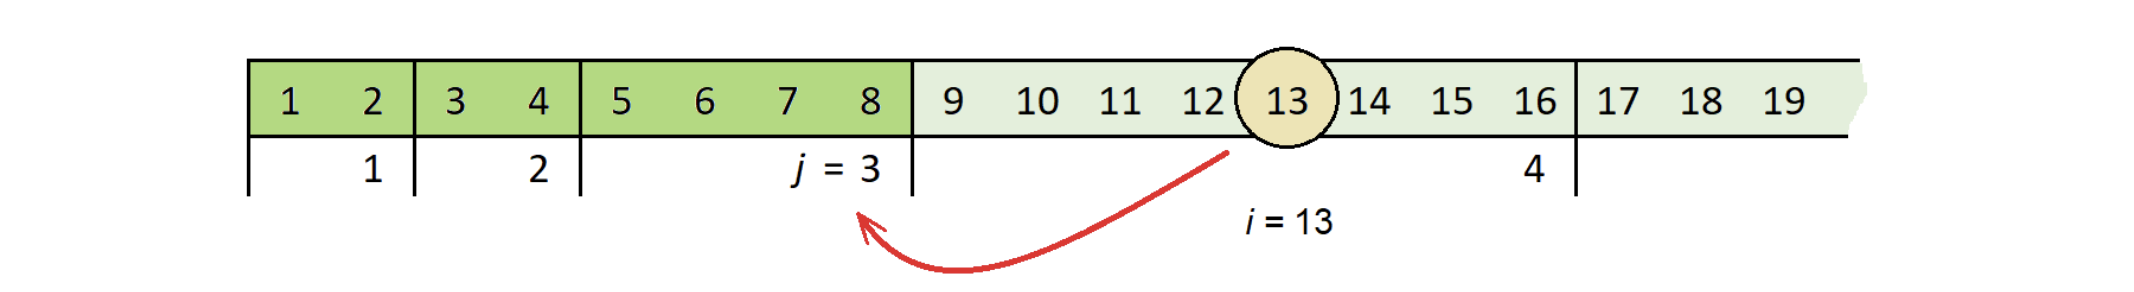
\includegraphics[width=15cm]{chapters/boosting/images/ordered_boost.png}

\subsection*{Модифицированный алгоритм градиентного бустинга в CatBoost}

\begin{tcolorbox}[colback=Lavender!10, colframe=Lavender]
\begin{enumerate}
\item Сгенерировать случайные перестановки \(\sigma_0, \sigma_1, \ldots, \sigma_s\);

\item \textbf{для всех} \(t = 1, \ldots, T\):
\begin{enumerate}
    \item выбрать перестановку \(\sigma_r\) случайно из \(\sigma_1, \ldots, \sigma_s\);
    \begin{flalign*}
    & g_{ti}^r := -\mathcal{L}'\left(a_{t-1}^{rj}(x_i), y_i\right) \quad \text{— несмещённый антиградиент;} &
    \end{flalign*}
    \begin{flalign*}
    & b_t := \arg\min_b \sum_{i=1}^{\ell} \left(b(x_i) - g_{ti}^r\right)^2; &
    \end{flalign*}
    \textbf{для всех} деревьев \(b_t^{rj}\), \(r = 1, \ldots, s\), \(2^j \leq \ell\):
    \begin{itemize}
        \item скопировать общую для них структуру дерева из \(b_t\);
        \item вычислить в листах \(b_t^{rj}\) средние по \(\{g_{ti}^r: x_i \in X^{rj}\}\);
    \end{itemize}
    \item вычислить в листах \(b_t\) средние по \(\{g_{ti}^0: x_i \in X^{0j}\}\);
    \item \textbf{GB part:} вычислить \(\alpha_t\) и обновить \(a_{t,i} := a_{t-1,i} + \alpha_t b_t(x_i)\);
\end{enumerate}
\end{enumerate}
\end{tcolorbox}

\subsection*{Обработка категориальных фичей}

Пусть $V$ — множество значений признака $f(x)$.\\

\textbf{Стандартные методы} либо громоздкие, либо переобучаются:
\begin{itemize}
    \item бинализация (one-hot encoding): \( b_v(x) = [f(x) = v] \);
    \item группирование (кластеризация) значений (LightGBM);
    \item статистика по целевому признаку - Target Statistics (TS):
    \begin{flalign*}
    & \tilde{f}(x_i) = \frac{\sum_{k=1}^{\ell}[f(x_k) = f(x_i)]y_k + \gamma p}{\sum_{k=1}^{\ell}[f(x_k) = f(x_i)] + \gamma} &
    \end{flalign*}
\end{itemize}

\textbf{CatBoost:}
\begin{itemize}
    \item статистика TS вычисляется по перестановкам \( X^{rj} \):
    $$
    \tilde{f}(x_i) = \frac{\sum_{x_k \in X^{rj}}[f(x_k) = f(x_i)]y_k + \gamma p}{\sum_{x_k \in X^{rj}}[f(x_k) = f(x_i)] + \gamma}, \quad j = \lfloor \log_2(i - 1) \rfloor
    $$
    \item конъюнкции категориальных признаков создаются «налёту» в процессе построения деревьев.
\end{itemize}

\subsection*{Особенности построения деревьев в CatBoost (Oblivious Decision Tree)}

Одной из ключевых особенностей алгоритма CatBoost является инновационный подход к построению деревьев решений. Деревья в CatBoost формируются по слоям, придерживаясь принципа: \textbf{\textit{все вершины одного уровня имеют одинаковый предикат}}. Это означает, что на каждом уровне дерева используется идентичный сплит для всех его вершин. Данный метод позволяет избавиться от сложных ветвлений в коде инференса модели и вместо этого использовать более эффективные битовые операции. Такое усовершенствование существенно ускоряет применение модели, особенно при работе с батчами данных.

Дерево глубины $H$, $D_v = \{0, 1\}$, для всех узлов уровня $h$ условие ветвления $f_h(x)$ одинаково; на уровне $h$ ровно $2^{h-1}$ вершин, $X$ делится на $2^H$ ячеек.

Классификатор задаётся \textit{таблицей решений} $B: \{0,1\}^H \to Y$:
$$
a(x) = B(f_1(x), \ldots, f_H(x)).
$$

\begin{figure}[ht]
    \centering
    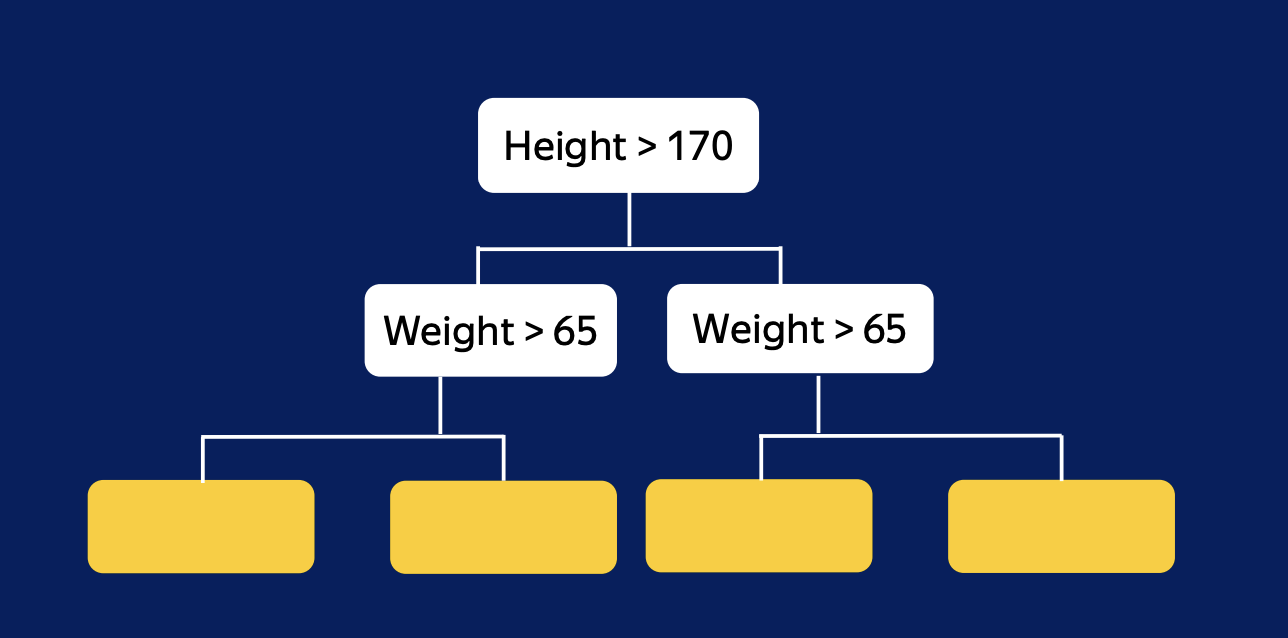
\includegraphics[width=15cm]{chapters/boosting/images/Tree.png}
    \caption{Пример сплита в слоях дерева в CatBoost}
\end{figure}

Кроме того, этот способ служит мощным средством регуляризации, обеспечивающим устойчивость модели к переобучению. Также данный подход позволяет всегда строить полные бинарные деревья (аналогично XGBoost, с тем различием, что CatBoost создаёт их даже в тех случаях, когда на некоторые поддеревья не попадает ни один объект из обучающей выборки). Основным критерием остановки процесса является ограничение на глубину деревьев.

\subsection*{Алгоритм обучения Oblivious Decision Tree}

\begin{tcolorbox}[colback=Lavender!10, colframe=Lavender]
\textbf{Вход:} выборка $X^\ell$; множество признаков $F$; глубина дерева $H$;\\
\textbf{Выход:} признаки $f_h, \ h = 1, \ldots, H$  таблица $B: \{0,1\}^H \to Y$;\\
\textbf{Для всех} $h = 1, \ldots, H$:\\
предикат с максимальным выигрышем определённости:
$$
f_h := \arg\max_{f \in \mathrm{bin}\{F\}} \text{Gain}(f_1, \ldots, f_{h-1}, f);
$$

\(\mathcal{B}(\beta) := \Phi(U_{H\beta}), \ \text{где} \ \Phi(U) = \text{avg}\{g_{ti}^r : x_i \in U\};\)
\end{tcolorbox}

$$
U_{h\beta} = \{x_i \in X^\ell : f_s(x_i) = \beta_s, \ s = 1 \ldots h\} \, \text{— выборка объектов } x_i,
\text{дошедших до вершины } \beta = (\beta_1, \ldots, \beta_h) \in \{0,1\}^h
$$

Выигрыш от ветвления на уровне \(h\) по всей выборке \(X^\ell\):
$$
\text{Gain}(f_1, \ldots, f_h) = \Phi(X^\ell) - \sum_{\beta \in \{0,1\}^h} \frac{|U_{h\beta}|}{\ell} \Phi(U_{h\beta})
$$

\subsection*{Основные преимущества CatBoost:}

\begin{itemize}
    \item \textbf{Эффективная работа с категориальными признаками.} CatBoost способен автоматически обрабатывать категориальные данные без необходимости их предварительного кодирования, такого как one-hot encoding.

    \item \textbf{Интегрированная обработка пропусков.} Алгоритм самостоятельно справляется с отсутствующими значениями.
    \item \textbf{Противодействие переобучению.} CatBoost применяет различные техники для предотвращения переобучения модели, включая мощные механизмы регуляризации и усреднение.

    \item \textbf{Высокая скорость и производительность.} В CatBoost реализованы множественные оптимизации, ускоряющие процесс обучения и предсказания. Он поддерживает многопоточную обработку и эффективно использует память.

    \item \textbf{Стабильность и воспроизводимость результатов.} Алгоритм гарантирует стабильные результаты даже при изменении порядка поступления входных данных, что важно для практического применения в реальных задачах.

\end{itemize}

\subsection*{Задача 1}

Предположим, что у вас есть обучающая выборка из 8 объектов. Покажите, как будут сформированы подвыборки $X^{rj} $ для объекта $x_5$ в одной из случайных перестановок, и какая модель будет использоваться для вычисления градиента на этом объекте.

\textbf{Решение:}

Используем одну случайную перестановку $\sigma$, которая для простоты совпадает с исходным порядком объектов: $\sigma = \left( x_1, \ x_2, \ x_3, \ x_4, \ x_5, \ x_6, \ x_7, \ x_8 \right)$.

\begin{enumerate}
\item  Определение значения $j$. Позиция объекта $x_5$ в перестановке: $i = 5$
   
   Вычисляем значение $j$:
   $$
   j = \left\lfloor \log_2(i - 1) \right\rfloor = \left\lfloor \log_2(5 - 1) \right\rfloor = \left\lfloor \log_2(4) \right\rfloor = 2
   $$
\item  Формирование подвыборки $X^{rj}$:

   Вычисляем размер подвыборки: $2^j = 2^2 = 4$

   Подвыборка $X^{rj}$ содержит первые $2^j = 4$ объекта из перестановки $\sigma$:
   $$
   X^{rj} = \left\{ x_1, \ x_2, \ x_3, \ x_4 \right\}
   $$

   Заметим, что объект $x_5$ не входит в эту подвыборку.
   
\item  Выбор модели для вычисления градиента на $x_5$:

   Модель $a_{t-1}^{rj}$ была обучена на подвыборке $X^{rj} = \left\{ x_1, \ x_2, \ x_3, \ x_4 \right\}$

   Поскольку $x_5 \notin X^{rj}$, модель $a_{t-1}^{rj}$ не была обучена на объекте $x_5$.

   Антиградиент на объекте $x_5$ вычисляется как:

   $$
   g_{t5}^r = -\mathcal{L}'\left( a_{t-1}^{rj}(x_5), \ y_5 \right)
   $$

   где \( a_{t-1}^{rj} \) — модель, обученная на подвыборке \( \left\{ x_1, \ x_2, \ x_3, \ x_4 \right\} \).

\end{enumerate}

\subsection*{Задача 2}

Опишите, как CatBoost вычисляет статистики по целевой переменной для категориальных признаков на примере:

\textbf{Дано}:
\begin{itemize}
    \item Перестановка объектов: $x_1, x_2, x_3, x_4, x_5, x_6$
    \item Значения признака  $f(x_i)$ и целевой переменной $y_i$
    \begin{table}[ht]
    \centering
    \begin{tabular}{c|c|c}
    Объект \( x_i \) & \( f(x_i) \) & \( y_i \) \\
    \hline
    \( x_1 \) & \( A \) & \( 1 \) \\
    \( x_2 \) & \( B \) & \( 0 \) \\
    \( x_3 \) & \( A \) & \( 1 \) \\
    \( x_4 \) & \( C \) & \( 0 \) \\
    \( x_5 \) & \( B \) & \( 1 \) \\
    \( x_6 \) & \( A \) & \( 0 \) \\
    \end{tabular}
    \end{table}
    \item Параметры: $\gamma = 1$, $p = 0{,}5$.
\end{itemize}

\textbf{Найти:} $\tilde{f}(x_5)$


\textbf{Решение:}

1. Определяем параметр $j$: 
$$
i = 5 \rightarrow j = \left\lfloor \log_2(i - 1) \right\rfloor = \left\lfloor \log_2(4) \right\rfloor = 2
$$

2. Формируем подвыборку $X^{rj}$:

   Количество объектов в подвыборке: $2^j = 2^2 = 4$. Значит, $X^{rj} = \{ x_1, \ x_2, \ x_3, \ x_4 \}$.

3. Выбираем объекты с \( f(x_k) = f(x_5) = B \):

   $\text{Совпадающие объекты} = x_2$, так как $f(x_2) = B$.

4. Получаем значения $y_k$ для совпадающих объектов: $y_2 = 0$.

5. Вычисляем сумму в числителе и знаменателе:
\begin{itemize}
   \item $\text{Числитель:} \sum\limits_{x_k \in X^{rj}} [f(x_k) = f(x_5)] y_k = y_2 = 0$
   \item $\text{Знаменатель:} \sum\limits_{x_k \in X^{rj}} [f(x_k) = f(x_5)] = 1$ 
\end{itemize}

6. Вычисляем $\tilde{f}(x_5)$:

$$
\tilde{f}(x_5) = \dfrac{\sum\limits_{x_k \in X^{rj}} [f(x_k) = f(x_5)] y_k + \gamma p}{\sum\limits_{x_k \in X^{rj}} [f(x_k) = f(x_5)] + \gamma} = \dfrac{0 + 1 \times 0{,}5}{1 + 1} = \dfrac{0{,}5}{2} = 0{,}25
$$

Ответ: $\tilde{f}(x_5) = 0{,}25$

\subsection*{Задача 3}

CatBoost использует особый тип деревьев решений, называемых небрежными деревьями (Oblivious Decision Trees), где на каждом уровне все узлы используют одинаковый предикат для разделения данных. Опишите основные преимущества использования обливиозных деревьев в CatBoost.

\textbf{Решение:}

\begin{enumerate}
    \item \textbf{Ускорение инференса:}
    \begin{itemize}
        \item Благодаря симметричной структуре дерева и одинаковым предикатам на каждом уровне, вычисления при предсказании можно оптимизировать.
        \item Использование битовых векторов и операций позволяет быстро определять путь по дереву и получать предсказание из таблицы решений.
    \end{itemize}
    \item \textbf{Оптимизация кода:}
    \begin{itemize}
        \item Упрощённая структура дерева снижает сложность кода и количество условных операторов.
        \item Это приводит к более эффективному использованию процессорного конвейера и кэшей.
    \end{itemize}
    \item \textbf{Регуляризация и устойчивость к переобучению:}
    \begin{itemize}
        \item Ограничение модели фиксированными предикатами на уровне уменьшает её сложность.
        \item Это служит формой регуляризации, помогая предотвратить переобучение на обучающей выборке.
    \end{itemize}
    \item \textbf{Предсказуемость и воспроизводимость:}
    \begin{itemize}
        \item Симметричная структура обеспечивает стабильность модели при различных изменениях в данных.
        \item Лёгкость воспроизведения результатов в различных средах и на различных устройствах.
    \end{itemize}
    \item \textbf{Совместимость с обработкой категориальных признаков:}
    \begin{itemize}
        \item Обливиозные деревья хорошо интегрируются с методами обработки категориальных признаков в CatBoost.
        \item Позволяют эффективно использовать конъюнкции (сочетания) признаков для повышения качества модели.
    \end{itemize}
\end{enumerate}

\section{LightGBM}

\subsection{Анализ сложности градиентного бустинга над решающими деревьями}

Самая вычислительно сложная часть градиентного бустинга над решающими деревьями (GBDT) является поиск наилучшей точки разбиения. В LightGBM используется \textbf{histogram-based} подход. Он заменяет истинные значения непрерывных признаков на группы ("бины") и для каждого признака строит гистограмму, где подсчитываются суммы весов для каждого бина. Вычислительная сложность в таком случае оказывается равной $\mathcal{O}(\#\text{bin}\cdot\#\text{features})$, что оказывается гораздо выгоднее алгоритма предварительной сортировки ($\mathcal{O}(\#\text{data}\cdot\#\text{features})$), поскольку обычно $\#\text{bin} \ll \#\text{data}$.

\subsection{Gradient-based One-Side Sampling (GOSS)}

Идея заключается в том, чтобы придумать способ, с помощью которого мы смогли бы находить наилучшее разбиение, не просматривая всю выборку. Аналогично алгоритму AdaBoost мы хотим присвоить каждому элементу выборки "вес", чтобы акцентировать внимание модели на них. В качестве этого веса может выступать градиент элемента. Так, например, данные с маленькими (по абсолютному значению) градиентами вносят малый вклад в ошибку, поэтому необязательно использовать их все.

GOSS предлагает следующий алгоритм сэмплирования: GOSS сначала сортирует данные в убывающем порядке по абсолютному значению градиентов и выбирает топ $a\times 100\%$ элементов. Далее он рандомно сэмплирует $b\times100\%$ элементов. Далее GOSS умножает часть с маленькими градиентами на константу $\frac{1 - a}{b}$ при вычислении прироста информации.

Более строго GBDT пытается выучить отображение из исходного пространства $\mathcal{X}^s$ в пространство градиентов $\mathcal{G}$. Предположим, мы имеем $n$ одинаковых независимо распределенных элементов $\{x_1, x_2, \ldots, x_n\}, \ x_i \in \mathcal{X}^s \ \forall i = \overline{1,n}$. Для каждой итерации градиентного бустинга определим $\{g_1, g_2, \ldots, g_n\}$ - антиградиенты loss-функции по отношению к текущему предсказанию модели. 

\par \textbf{Определение.} Пусть $\mathcal{X}$ - обучающая выборка в текущей ноде решающего дерева. Тогда прирост информации при разделении признака $j$ по значению $d$ для этой ноды определяется как

\begin{equation*}
    V_{j|\mathcal{X}}(d) = \frac{1}{|\mathcal{X}|}\left(\frac{\left(\sum\limits_{x_i\in \mathcal{X}: x_{ij} \leqslant d}g_i\right)^2}{n^j_l(d)} + \frac{\left(\sum\limits_{x_i\in \mathcal{X}: x_{ij} > d}g_i\right)^2}{n^j_r(d)}\right)
\end{equation*}

где $n^j_l(d) = |x_i\in \mathcal{X}: x_{ij} \leqslant d|, \ n^j_r(d) = |x_i\in \mathcal{X}: x_{ij} > d|$ Для каждого признака $j$ алгоритм выбирает $d_j^* = \arg\max\limits_dV_j(d)$ и вычисляет наибольший прирост информации $V_j(d_j^*)$. Далее данные делятся по признаку $j^*$ и по значению $d_j^*$ на правое и левое поддервья. В предложенном GOSS алгоритме выберем топ $a\times100\%$ элементов с наибольшим градиентом (по абсолютному значению) и обозначим это множество $A$. Далее из $\overline{A}$ случайно выберем $b\times|\overline{A}|$ элементов и обозначим $B$. Тогда оценка прироста информации имеет вид

\begin{equation*}
    \widetilde{V}_j(d) = \frac{1}{|\mathcal{X}|}\left(\frac{\left(\sum\limits_{x_i\in A_l}g_i + \frac{1 - a}{b}\sum\limits_{x_i\in B_l}g_i\right)^2}{n^j_l(d)} + \frac{\left(\sum\limits_{x_i\in A_r}g_i + \frac{1 - a}{b}\sum\limits_{x_i\in B_r}g_i\right)^2}{n^j_r(d)}\right),
\end{equation*}

где $A_l = \{x_i \in A: x_{ij} < d\}, \ A_r = \{x_i \in A: x_{ij} > d\}, B_l = \{x_i \in B: x_{ij} \leqslant d\}, \ B_r = \{x_i \in B: x_{ij} > d\}$.

То есть в GOSS мы используем оценку прироста информации $\widetilde{V}_j(d)$, рассчитанную по меньшему датасету, нежели точную $V_j(d)$. При этом согласно утверждению следующей теоремы, используя оценку $\widetilde{V}_j(d)$ вместо $V_j(d)$ мы не сильно проигрывает в точности:

\par \textbf{Теорема.} Обозначим ошибку аппроксимации GOSS как $\varepsilon (d) = |\widetilde{V}_j(d) - V_j(d)|$ и $\overline{g}_l^j(d) = \frac{\sum\limits_{x_i \in \mathcal{X}_l}|g_i|}{n^j_l(d)}, \ \overline{g}_r^j(d) = \frac{\sum\limits_{x_i \in \mathcal{X}_r}|g_i|}{n^j_r(d)}$. Тогда с вероятностью хотя бы $1 - \delta$ имеет место оценка

\begin{equation*}
    \varepsilon(d) \leqslant C_{a, b}^2 \ln \frac{1}{\delta} \cdot \max \left\{\frac{1}{n^j_l(d)}, \frac{1}{n^j_r(d)}\right\} + 2DC_{a, b}\sqrt{\frac{\ln \frac{1}{\delta}}{n}},
\end{equation*}

где $C_{a. b} = \frac{1 - a}{\sqrt{b}}\max_{x_i \in \overline{A}}|g_i|$ и $D = \max\left\{\overline{g}_l^j(d), \overline{g}_r^j(d)\right\}$. 

Из данной теоремы следует асимптотическая оценка GOSS $\mathcal{O}\left(\frac{1}{n^j_l(d)} + \frac{1}{n^j_r(d)} + \frac{1}{\sqrt{n}}\right)$. Поэтому если разбиения будут не слишком несбалансированными (то есть $n^j_l(d) \geqslant \mathcal{O}(\sqrt{n})$ и $n^j_r(d) \geqslant \mathcal{O}(\sqrt{n})$), то общая асимптотика будет составлять $\mathcal{O}\left(\frac{1}{\sqrt{n}}\right) \underset{n\rightarrow \infty}{\rightarrow} 0$. То есть при большом количестве данных приближение будет достаточно точным.

Обобщающая способность GOSS будет также близка к алгоритму с "честным" приростом информации. $\varepsilon_{\text{gen}}^{\text{GOSS}}(d) = |\widetilde{V}_j(d) - V_*(d)| \leqslant |\widetilde{V}_j(d) - V_j(d)| + |V_j(d) - V_*(d)| = \varepsilon_{\text{GOSS}}(d) + \varepsilon_{\text{gen}}(d)$.


\subsection{Exclusive Feature Bundling (EFB)}

Зачастую, датасеты большой размерности являются сильно разреженными, возникает мысль, что возможно уменьшить количество признаков, не сильно теряя при этом в точности. В частности, в разреженном пространстве зачастую встречаются взаимоисключающие признаки, то есть признаки, которые не могут быть ненулевыми одновременно. Такие признаки можно объединить в один (exclusive feature bundle). Соответственно, гистограмма из подпункта \textbf{1.1}, построенная на этих объединенных признаках имеет асимптотику $\mathcal{O}(\#\text{data}\times\#\text{bundle})$, вместо $\mathcal{O}(\#\text{data}\times\#\text{feature})$, что значительно быстрее при $\text{\#bundle} \ll \#\text{feature}$.

Сведем задачу разделения на такие $\text{bundle}$ к задаче раскраски графа (NP-Hard), признаки будем считать вершинами и ребро будем проводить между признаками, которые не являются взаимоисключающими. Точного полиномиального решения на текущий момент не существует, тем не менее задачу можно достаточно хорошо решить с помощью жадного алгоритма. Более того, обычно существует довольно много признаков, которые хотя и не являются на 100\% взаимоисключающими, но редко принимают ненулевые значения одновременно. Если наш алгоритм сможет разрешить небольшую долю конфликтов, мы сможем мы сможем получить еще меньшее количество bundles признаков и еще больше повысить эффективность вычислений. Такая процедура повлияет на точность при обучении не более чем $\mathcal{O}\left([(1-\gamma)n]^{\frac{2}{3}}\right)$, где $\gamma$ - максимальная частота конфликтов в каждом bundle.

Сформулируем итоговый алгоритм. Строим граф признаков с весами на ребрах, соответствующими общему числу конфликтов между признаками. Далее сортируем признаки по количеству соседей, с которыми есть конфликты в убывающем порядке, наконец, для каждого признака из упорядоченного списка проверяется, можно ли добавить признак в существующие bundles с минимальным конфликтом (контролируется параметром $\gamma$), иначе создается новый bundle. Общая сложность алгоритма - $\mathcal{O}(\#\text{feature}^2)$.

Далее нам надо понять, как правильно объединять признаки в один bundle, то есть по значению признака в bundle мы должны уметь определить исходное значение объединенных признаков. Это может быть сделано с помощью добавления смещения к признакам. Например, признак $A$ принимает значения из диапазона $[0, 10)$, а признак $B$ - из $[0, 20)$. Добавим смещение признаку $B$, теперь он принимает значения из диапазона $[10, 30)$. После объединения признаков $A$ и $B$ полученный признак будет принимать значения в диапазоне $[0, 30)$.

\subsection{Задачи}

\begin{enumerate}
    \item Обычно в методах градиентного бустинга стараются строить неглубокие деревья, чтобы не переобучиться на обучающей выборке и ускорить время обучения. Сохраняется ли это в LightGBM? Почему?

    Ответ: Нет, это нарушается в LightGBM реализации градиентного бустинга. Дело в другой стратегии роста - $\text{leaf-wise growth}$. Глядя на функционал прироста информации видно, что каждый раз выборка делится на одну часть с большими градиентами и вторую часть, с маленькими градиентами. Данные с маленькими градиентами уже вносят малый вклад в ошибку и дальше разбивать их не так информативно. LightGBM на каждом шаге выбирает наиболее оптимальное разбиение, не обращая внимание на сбалансированность получающегося дерева, из-за чего зачастую получаются глубокие и несбалансированные деревья.

    \item В GOSS при подсчете оценки прироста информации мы домножаем на множитель $\frac{1-a}{b}$. Зачем это нужно и что будет, если это домножение не производить?

    Ответ: Если мы просто уменьшим количество данных с малыми градиентами, это исказит относительную важность этих объектов в функции потерь. Масштабирование градиентов увеличивает вклад выбранных объектов с малыми градиентами так, чтобы их совокупный эффект оставался пропорциональным их изначальной доле в данных. Если множитель не использовать, объекты с большими градиентами будут еще сильнее доминировать при построении дерева. Модель будет чрезмерно подстраиваться под сложные примеры, пренебрегая общей точностью и, скорее всего, ухудшая обобщающую способность.

    \item В чем важность параметра $\text{min\_data\_in\_leaf}$ параметра в LightGBM, к чему могут привести его высокие и низкие значения? А параметра \newline $\text{num\_leaves}$?

    Ответ: \begin{enumerate}
        \item $\text{min\_data\_in\_leaf}$ - отвечает за минимальное количество элементов выборки в каждом листе. Чем выше этот параметр, тем более модель устойчива к зашумленным данным. Слишком большие значения, однако, могут приводить к снижению чувствительности модели сложных зависимостей, ухудшая качество предсказания. Слишком малые значения параметра, напротив, позволяют выучить достаточно сложные зависимости, однако возрастает вероятность переобучения.

        \item $\text{num\_leaves}$ - отвечает за максимальное количество листьев дерева. Аналогично предыдущему признаку регулирует сложность модели. Чем больше листьев - тем более сложные зависимости между признаками и целевой переменной может улавливать дерево, однако высока вероятность переобучиться. И напротив, чем меньше листьев, тем модель более устойчива к переобучению и к шума и тем хуже она справляется со сложными зависимостями.
    \end{enumerate}
\end{enumerate}

    \clearpage
    \chapter{Байесовская теория классификации}
    
\section*{Разложение на смещение и разброс}


\subsection*{Теория}

Допустим, у нас есть некоторая выборка, на которой линейные методы работают лучше решающих деревьев с точки зрения ошибки на контроле. Почему это так? Чем можно объяснить превосходство определённого метода обучения? Оказывается, ошибка любой модели складывается из трёх факторов: сложности самой выборки, схожести модели с истинной зависимостью ответов от объектов в выборке, и богатства семейства, из которого выбирается конкретная модель. Между этими факторами существует некоторый баланс, и уменьшение одного из них приводит к увеличению другого. Такое разложение ошибки носит название разложения на смещение и разброс, и его формальным выводом мы сейчас займёмся.

\vspace*{0.4cm}

Пусть задана выборка $X = (x_i, y_i)_{i=1}^n$ с вещественными ответами $y_i \in \mathbb{R}$ (рассматриваем задачу регрессии). Будем считать, что на пространстве всех объектов и ответов $X \times Y$ существует распределение $p(x, y)$, из которого сгенерирована выборка $X$ и ответы на ней.

Рассмотрим квадратичную функцию потерь
\[
L(y, a) = (y - a(x))^2
\]
и соответствующий ей среднеквадратичный риск
\[
R(a) = \mathbb{E}_{x, y} \left[ (y - a(x))^2 \right] = \int_{X} \int_{Y} p(x, y) (y - a(x))^2 dxdy.
\]

Данный функционал усредняет ошибку модели в каждой точке пространства $x$ и для каждого возможного ответа $y$, причём вклад пары $(x, y)$, по сути, пропорционален вероятности получить её в выборке $p(x, y)$. Разумеется, на практике мы не можем вычислить данный функционал, поскольку распределение $p(x, y)$ неизвестно. Тем не менее, в теории он позволяет измерить качество модели на всех возможных объектах, а не только на наблюдённой выборке.

\subsection*{Задание}

Покажите, что минимум среднеквадратичного риска достигается на функции, возвращающей условное математическое ожидание ответа при фиксированном объекте.

\[
a_*(x) = \mathbb{E}[y \mid x] = \int_Y y p(y \mid x) dy = \arg \min_a R(a).
\]

Иными словами покажите, что мы должны провести «взвешенное голосование» по всем возможным ответам, при этом веса ответа равны апостериорной вероятности.

\subsection*{Решение}

Преобразуем функцию потерь:

\[
L(y, a(x)) = (y - a(x))^2 = (y - \mathbb{E}(y \mid x) + \mathbb{E}(y \mid x) - a(x))^2 =
\]
\[
= (y - \mathbb{E}(y \mid x))^2 + 2(y - \mathbb{E}(y \mid x))(\mathbb{E}(y \mid x) - a(x)) + (\mathbb{E}(y \mid x) - a(x))^2.
\]

Подставляя её в функционал среднеквадратичного риска, получаем:

\[
R(a) = \mathbb{E}_{x,y}[L(y, a(x))] = 
\]
\[
= \mathbb{E}_{x,y}[(y - \mathbb{E}(y \mid x))^2] + \mathbb{E}_{x,y}[(\mathbb{E}(y \mid x) - a(x))^2] +
2 \mathbb{E}_{x,y}[(y - \mathbb{E}(y \mid x))(\mathbb{E}(y \mid x) - a(x))].
\]

Разберёмся сначала с последним слагаемым. Перейдём от матожидания \(\mathbb{E}_{x,y}[f(x, y)]\) к цепочке матожиданий:

\[
\mathbb{E}_x \mathbb{E}_y[f(x, y) \mid x] = \int_X \left( \int_Y f(x, y) p(y \mid x) dy \right) p(x) dx
\]

и заметим, что величина \((\mathbb{E}(y \mid x) - a(x))\) не зависит от \(y\), и поэтому её можно вынести за матожидание по \(y\):

\[
\mathbb{E}_x \mathbb{E}_y \left[ (y - \mathbb{E}(y \mid x))(\mathbb{E}(y \mid x) - a(x)) \mid x \right] =
\]
\[
= \mathbb{E}_x \left( (\mathbb{E}(y \mid x) - a(x)) \mathbb{E}_y \left[ (y - \mathbb{E}(y \mid x)) \mid x \right] \right) =
\]
\[
= \mathbb{E}_x \left( (\mathbb{E}(y \mid x) - a(x)) (\mathbb{E}_y[y \mid x] - \mathbb{E}_y \mathbb{E}(y \mid x)) \right) =
\]
\[
= 0.
\]

Получаем, что функционал среднеквадратичного риска имеет вид:

\[
R(a) = \mathbb{E}_{x,y}(y - \mathbb{E}(y \mid x))^2 + \mathbb{E}_{x,y}((\mathbb{E}(y \mid x) - a(x))^2).
\]

От алгоритма \(a(x)\) зависит только второе слагаемое, и оно достигает своего минимума, если \(a(x) = \mathbb{E}(y \mid x)\). Таким образом, оптимальная модель регрессии для квадратичной функции потерь имеет вид:

\[
a_*(x) = \mathbb{E}(y \mid x) = \int_Y y p(y \mid x) dy.
\]

Что и требовалось показать.


\subsection*{Теория}

Для того, чтобы построить идеальную функцию регрессии, необходимо знать распределение на объектах и ответах $p(x, y)$, что, как правило, невозможно. На практике вместо этого выбирается некоторый \emph{метод обучения} $\mu : (\mathbb{X} \times \mathbb{Y})^\ell \to A$, который произвольной обучающей выборке ставит в соответствие некоторый алгоритм из семейства $A$. В качестве меры качества метода обучения можно взять усредненный по всем выборкам среднеквадратичный риск алгоритма, выбранного методом $\mu$ по выборке:
\newpage
\[
    L(\mu) = \mathbb{E}_X \left[ \mathbb{E}_{x, y} \left[ \left( y - \mu(X)(x) \right)^2 \right] \right] = \tag{1}
\]
\[  
    =\int_{(\mathbb{X} \times \mathbb{Y})^\ell} \int_{\mathbb{X} \times \mathbb{Y}} (y - \mu(X)(x))^2 
    p(x, y) \prod_{i=1}^\ell p(x_i, y_i) dx dy dx_1 dy_1 \ldots dx_\ell dy_\ell.
\]

Здесь матожидание $\mathbb{E}_X[\cdot]$ берется по всем возможным выборкам $\{(x_1, y_1), \ldots, (x_\ell, y_\ell)\}$ из распределения $\prod_{i=1}^\ell p(x_i, y_i)$.

Обратим внимание, что результатом применения метода обучения $\mu(X)$ к выборке $X$ является модель, поэтому правильно писать $\mu(X)(x)$. Но это довольно громоздкая запись, поэтому будем везде дальше писать просто $\mu(X)$, но не будем забывать, что это функция, зависящая от объекта $x$.

Среднеквадратичный риск на фиксированной выборке $X$ можно расписать как:
\[
\mathbb{E}_{x, y} \left[ \left( y - \mu(X) \right)^2 \right] = 
\mathbb{E}_{x, y} \left[ \left( y - \mathbb{E}[y \mid x] \right)^2 \right] + 
\mathbb{E}_{x, y} \left[ \left( \mathbb{E}[y \mid x] - \mu(X) \right)^2 \right].
\]

\subsection*{Задание}

Подставим это представление в (1):
\[
L(\mu) = \mathbb{E}_X \left[ \mathbb{E}_{x,y} \left[ \left( y - \mathbb{E}[y \mid x] \right)^2 \right] 
+ \mathbb{E}_{x,y} \left[ \left( \mathbb{E}[y \mid x] - \mu(X) \right)^2 \right] \right] =
\]
\[
= \mathbb{E}_{x,y} \left[ \left( y - \mathbb{E}[y \mid x] \right)^2 \right] 
+ \mathbb{E}_{x,y} \left[ \mathbb{E}_X \left[ \left( \mathbb{E}[y \mid x] - \mu(X) \right)^2 \right] \right]. \tag{2}
\]

Преобразуем второе слагаемое:
\[
\mathbb{E}_{x,y} \left[ 
\mathbb{E}_X \left[ \left( \mathbb{E}[y \mid x] - \mu(X) \right)^2 \right] \right] = \]
\[
= \mathbb{E}_{x,y} \left[ 
\mathbb{E}_X \left[ \left( \mathbb{E}[y \mid x] - 
\mathbb{E}_X[\mu(X)] + \mathbb{E}_X[\mu(X)] - \mu(X) \right)^2 \right] \right] =
\]
\[
= \mathbb{E}_{x,y} \left[ 
\mathbb{E}_X \left[ \left( \mathbb{E}[y \mid x] - \mathbb{E}_X[\mu(X)] \right)^2 \right] \right] 
+ \mathbb{E}_{x,y} \left[ 
\mathbb{E}_X \left[ \left( \mathbb{E}_X[\mu(X)] - \mu(X) \right)^2 \right] \right] +
\tag{3}\]
\[
+ 2 \mathbb{E}_{x,y} \left[ 
\mathbb{E}_X \left[ \left( \mathbb{E}[y \mid x] - \mathbb{E}_X[\mu(X)] \right) 
\left( \mathbb{E}_X[\mu(X)] - \mu(X) \right) \right] \right].
\]

Покажите, что последнее слагаемое обращается в нуль.

\subsection*{Решение}

Покажем, что последнее слагаемое обращается в нуль:
\[
\mathbb{E}_X \left[ \left( \mathbb{E}[y \mid x] - \mathbb{E}_X \left[ \mu(X) \right] \right) 
\left( \mathbb{E}_X \left[ \mu(X) \right] - \mu(X) \right) \right] =
\]
\[
= \left( \mathbb{E}[y \mid x] - \mathbb{E}_X \left[ \mu(X) \right] \right) 
\mathbb{E}_X \left[ \mathbb{E}_X \left[ \mu(X) \right] - \mu(X) \right] =
\]
\[
= \left( \mathbb{E}[y \mid x] - \mathbb{E}_X \left[ \mu(X) \right] \right) 
\left[ \mathbb{E}_X \mu(X) - \mathbb{E}_X \mu(X) \right] =
\]
\[
= 0.
\]

\subsection*{Задание}

Используя результаты предыдущих задач и подставляя (3) в (2) получите выражение для $L(\mu)$, укажите слагаемые, отвечающие за \emph{смещение}, \emph{шум} и \emph{разброс}.

\newpage

\subsection*{Решение}

Подставим выражение (3) в (2), учитывая результаты предыдущих задач:

\[
L(\mu) = \underbrace{\mathbb{E}_{x, y} \left[ \left( y - \mathbb{E}[y \mid x] \right)^2 \right]}_{\text{шум}}
+ \underbrace{\mathbb{E}_x \left[ \left( \mathbb{E}_X [\mu(X)] - \mathbb{E}[y \mid x] \right)^2 \right]}_{\text{смещение}}
+ \underbrace{\mathbb{E}_x \left[ \mathbb{E}_X \left[ \left( \mu(X) - \mathbb{E}_X[\mu(X)] \right)^2 \right] \right]}_{\text{разброс}}.
\]

Рассмотрим подробнее компоненты полученного разложения ошибки. Первая компонента характеризует \emph{шум} (\emph{noise}) в данных и равна ошибке идеального алгоритма. Невозможно построить алгоритм, имеющий меньшую среднеквадратичную ошибку. Вторая компонента характеризует \emph{смещение} (\emph{bias}) метода обучения, то есть отклонение среднего ответа обученного алгоритма от ответа идеального алгоритма. Третья компонента характеризует \emph{дисперсию} (\emph{variance}), то есть разброс ответов обученных алгоритмов относительно среднего ответа.

\section*{Линейный дискриминант Фишера}

Линейный дискриминант Фишера в первоначальном значении — метод, определяющий расстояние между распределениями двух разных классов объектов или событий. Он может использоваться в задачах машинного обучения при статистическом (байесовском) подходе к решению задач классификации. 

Предположим, что обучающая выборка удовлетворяет помимо базовых гипотез байесовского классификатора также следующим гипотезам:
\begin{itemize}
    \item Классы распределены по нормальному закону.
    \item Матрицы ковариаций классов равны.
\end{itemize}

Такой случай соответствует наилучшему разделению классов по дискриминанту Фишера (в первоначальном значении). Тогда статистический подход приводит к линейному дискриминанту, и именно этот алгоритм классификации в настоящее время часто понимается под термином линейный дискриминант Фишера.

\subsection*{Введение}

При некоторых общих предположениях байесовский классификатор сводится к формуле:
\[ 
a(x) = \mathrm{arg}\max_{yin Y} \lambda_{y} P_y p_y(x), 
\]
где $Y$ — множество ответов (классов), $x$ принадлежит множеству объектов $X$, $P_y$ — априорная вероятность класса $y$, $p_y(x)$ — функция правдоподобия класса $y$, $\lambda_{y}$ — весовой коэффициент (цена ошибки на объекте класса $y$).

При выдвижении всех указанных выше гипотез, кроме гипотезы о равенстве матриц ковариаций, данная формула принимает вид:
\[
a(x) = \mathrm{arg}\max_{yin Y} \left( ln(\lambda_{y} P_y) - \frac{1}{2}(x - \mu_y)^T \Sigma^{-1}_{y} (x - \mu_y) - \frac{1}{2}ln(\det{\Sigma^{-1}_{y}}) - \frac{n}{2}ln(2\pi) \right),
\]
где 
\[
\mu_y = \frac{1}{l_y} \sum^{l}_{\stackrel{i=1}{y_i = y}}x_i, \quad 
\Sigma_y = \frac{1}{l_y} \sum^{l}_{\stackrel{i=1}{y_i = y}}(x_i - \mu_y)(x_i - \mu_y)^T
\]
— приближения вектора математического ожидания и матрицы ковариации класса $y$, полученные как оценки максимума правдоподобия, $l$ — длина обучающей выборки, $l_y$ — количество объектов класса $y$ в обучающей выборке, $x \in \mathbb{R}^n$.

Данный алгоритм классификации является квадратичным дискриминантом. Он имеет ряд недостатков, одним из самых существенных из которых является плохая обусловленность или вырожденность матрицы ковариаций $\Sigma_y$ при малом количестве обучающих элементов класса $y$, вследствие чего при обращении данной матрицы $\Sigma^{-1}_{y}$ может получиться сильно искаженный результат, и весь алгоритм классификации окажется неустойчивым, будет работать плохо (возможна также ситуация, при которой обратная матрица $\Sigma^{-1}_{y}$ вообще не будет существовать). Линейный дискриминант Фишера решает данную проблему.

\textbf{Задача 1.} Каковы преимущества и недостатки использования квадратичного дискриминантного анализа (QDA) по сравнению с линейным дискриминантным анализом (LDA) в задачах классификации?


\subsection*{Основная идея алгоритма}

При принятии гипотезы о равенстве между собой ковариационных матриц алгоритм классификации принимает вид:
\[
a(x) = \mathrm{arg}\max_{yin Y} \left( ln(\lambda_{y} P_y) - \frac{1}{2}\mu_{y}^{T} \Sigma^{-1} \mu_y + x^T \Sigma^{-1} \mu_y \right),
\]
или 
\[
a(x) = \mathrm{arg}\max_{y\in Y} (\beta_y + x^T\alpha_y).
\]

Простота классификации линейным дискриминантом Фишера — одно из достоинств алгоритма: в случае с двумя классами в двумерном признаковом пространстве разделяющей поверхностью будет прямая. Если классов больше двух, то разделяющая поверхность будет кусочно-линейной. Но главным преимуществом алгоритма по сравнению с квадратичным дискриминантом является уменьшение эффекта плохой обусловленности ковариационной матрицы при недостаточных данных.

При малых $l_y$ приближения 
\[
\Sigma_y = \frac{1}{l_y} \sum^{l}_{\stackrel{i=1}{y_i = y}}(x_i - \mu_y)(x_i - \mu_y)^T
\]
дадут плохой результат, поэтому даже в тех задачах, где заведомо известно, что классы имеют различные формы, иногда бывает выгодно воспользоваться эвристикой дискриминанта Фишера и считать матрицы ковариаций всех классов одинаковыми. Это позволит вычислить некоторую "среднюю" матрицу ковариаций, используя всю выборку:
\[
\Sigma = \frac{1}{l} \sum^{l}_{i=1}(x_i - \mu_{y_i})(x_i - \mu_{y_i})^T,
\]
использование которой в большинстве случаев сделает алгоритм классификации более устойчивым.

\textbf{Задача 2.} Каковы основные предпосылки и ограничения линейного дискриминанта Фишера, и в каких случаях его применение может быть предпочтительнее по сравнению с квадратичным дискриминантом?

\subsection*{Выводы}

Эвристика линейного дискриминанта Фишера является в некотором роде упрощением квадратичного дискриминанта. Она используется с целью получить более устойчивый алгоритм классификации. Наиболее целесообразно пользоваться линейным дискриминантом Фишера, когда данных для обучения недостаточно. Вследствие основной гипотезы, на которой базируется алгоритм, наиболее удачно им решаются простые задачи классификации, в которых по формам классы "похожи" друг на друга.

Процесс классификации линейным дискриминантом Фишера можно описать следующей схемой:
\begin{enumerate}
    \item Обучение
    \begin{itemize}
        \item Оценивание математических ожиданий $\mu_y$
        \item Вычисление общей ковариационной матрицы $\Sigma$ и ее обращение
    \end{itemize}
    
    \item Классификация
    \begin{itemize}
        \item Использование формулы 
        \[
        a(x) = \mathrm{arg}\max_{yin Y} \left( ln(\lambda_{y} P_y) - \frac{1}{2}\mu_{y}^{T} \Sigma^{-1} \mu_y + x^T \Sigma^{-1} \mu_y \right)
        \]
    \end{itemize}
\end{enumerate}

\textbf{Задача 3.}Даны два класса объектов, представленные следующими данными:

\begin{itemize}
    \item Класс 1: $X_1 = {(2, 3), (3, 3), (2, 4)}$
    \item Класс 2: $X_2 = {(5, 6), (6, 5), (5, 7)}$
\end{itemize}

Найдите линейный дискриминант Фишера
\newline

\textit{Ответ к задаче 1}
\begin{itemize}
    \item QDA лучше подходит для задач, где классы имеют разные дисперсии и формы, и когда доступно достаточно данных для надежной оценки параметров.

    \item LDA может быть предпочтительнее в случаях с ограниченным количеством данных или когда классы можно считать линейно разделимыми.
\end{itemize}

\textit{Ответ к задаче 2}
Основные предпосылки линейного дискриминанта Фишера:
\begin{itemize}
    \item Нормальность: Предполагается, что данные в каждом классе распределены нормально.

    \item Однородность дисперсий: Линейный дискриминант предполагает одинаковые матрицы ковариаций для всех классов.

    \item Линейная разделимость: Предполагается, что классы можно разделить линейной границей.
\end{itemize}
Ограничения:
\begin{itemize}
    \item Если данные не удовлетворяют предпосылкам нормальности или однородности дисперсий, производительность линейного дискриминанта может значительно ухудшиться.

    \item Линейный дискриминант не может захватить сложные нелинейные зависимости между классами.
\end{itemize}
Когда предпочтительнее:
\begin{itemize}
    \item Линейный дискриминант может быть предпочтительнее квадратичного в случаях, когда:

    \item Данные имеют высокую размерность и при этом имеют достаточно малое количество образцов (линейный подход менее подвержен переобучению).

    \item Классы действительно линейно разделимы или близки к этому.
\end{itemize}
\textit{Пример:} В задачах распознавания лиц с использованием признаков (например, цветовые компоненты пикселей) линейный дискриминант может быть эффективным из-за высокой размерности данных и необходимости в простоте модели.

\textit{Ответ к задаче 3}
\begin{enumerate}
    \item Найдите средние векторы для каждого класса.
    
    Средние векторы:
    \[
    \mu_1 = \left(\frac{2+3+2}{3}, \frac{3+3+4}{3}\right) = \left(2.33, 3.33\right)
    \]
    
    \[
    \mu_2 = \left(\frac{5+6+5}{3}, \frac{6+5+7}{3}\right) = \left(5.33, 6.00\right)
    \]
    
    \item Вычислите матрицы дисперсии для каждого класса.
    
    Для класса 1:
    \[
    S_1 = \frac{1}{n_1-1} \sum_{i=1}^{n_1} (x_i - \mu_1)(x_i - \mu_1)^T
    \]
    
    После вычислений получаем:
    \[
    S_1 = \begin{pmatrix}
        0.33 & 0.33 \
        0.33 & 0.67
    \end{pmatrix}
    \]

    Для класса 2:
    \[
    S_2 = \frac{1}{n_2-1} \sum_{i=1}^{n_2} (x_i - \mu_2)(x_i - \mu_2)^T
    \]
    
    После вычислений получаем:
    \[
    S_2 = \begin{pmatrix}
        0.67 & -0.33 \
        -0.33 & 0.67
    \end{pmatrix}
    \]

    \item Найдите линейный дискриминант Фишера.
    
    Сначала находим объединённую матрицу дисперсии:
    \[
    S_W = S_1 + S_2 =
    \begin{pmatrix}
        0.33 + 0.67 & 0.33 - 0.33 \
        0.33 - 0.33 & 0.67 + 0.67
    \end{pmatrix}
    =
    \begin{pmatrix}
        1 & 0 \
        0 & 1.34
    \end{pmatrix}
    \]

    Теперь находим весовой вектор $w$:
    \[
    w = S_W^{-1}(\mu_1 - \mu_2) =
    \begin{pmatrix}
        1 & 0 \
        0 & 1.34
    \end{pmatrix}^{-1}
    \begin{pmatrix}
        2.33 - 5.33 \
        3.33 - 6
    \end{pmatrix}
    =
    \begin{pmatrix}
        -3 \
        -2.67
    \end{pmatrix}
    \]
\end{enumerate}


\section*{Байесовские методы классификации}
Решаем задачу классификации. Пусть $A = A_1 \times \ldots \times A_m$ --- пространство объектов, $B$ --- конечное множество классов. Предположим, что объекты $(x, y) \in A \times B$ независимо выбираются из какого-то неизвестного распределения с обобщённой плотностью распределения $p(x, y)$. Пусть $(X, Y)$ --- случайная величина на $A \times B$ с таким распределением. Хотим по $x$ находить его наиболее вероятный класс, то есть класс $y$, максимизирующий $P(Y=y|X=x)$. По формуле Байеса $P(y|x)=\frac{P(y)p(x|y)}{p(x)}$, поэтому максимизация $P(y|x)$ равносильна максимизации $P(y)p(x|y)$. Таким образом, задача сводится к восстанавлению дискретного априорного распределения $P(y)$ и восстановлению условного распределения $p(x|y)$.

Обычно предполагается, что $Y$ имеет произвольное категориальное распределение на $B$, то есть что о распределении $Y$ нет никакой информации, кроме множества принимаемых значений. В этом случае можно аналитически найти оценку на параметры распределения $P(Y=b_i)$ методом максимального правдоподобия.

\textbf{Задача 1.} Пусть $N$ --- количество элементов в выборке. Для любого $b \in B$ обозначим через $N_b$ --- количество элементов, для которых $y=b$ и через $\overline{p_b}$ --- частоту, с которой $y$ принимает значение $b$, то есть $\overline{p_b} = \frac{N_b}{N}$. Докажите, что $\overline{p_b}$ --- оценка максимального правдоподобия вероятностей $P(Y=b)$. \\
\textit{Указание: перейдите к максимизации логарифма правдоподобия и воспользуйтесь неравенством Гиббса.}


\subsection*{Наивный Байесовский классификатор}

Наивный Байесовский классификатор делает предположение, что признаки независимы в совокупности при условии классов, то есть для любого $k$, любых $i_1 < \ldots < i_k$ и любых $x_1, \ldots, x_k, y$ выполнено $p(X_{i_1}=x_1, \ldots, X_{i_k} = x_k|Y=y)=p(X_{i_1}=x_1|Y=y)\cdot\ldots\cdot p(X_{i_k}=x_k|Y=y)$. Отметим, что треубется именно независимость $X_i$ при условии $Y$, а не просто независимость $X_i$.

\textbf{Задача 2.} \\
a) Приведите пример совместного распределения бернуллиевских случайных величин $X_1, X_2, Y$ при котором $X_1$ и $X_2$ независимы, но не независимы при условии $Y$. \\
b) Приведите пример совместного распределения бернуллиевских случайных величин $X_1, X_2, Y$ при котором $X_1$ и $X_2$ независимы при условии $Y$, но не независимы.

Для каждого класса $b \in B$ и для каждого признака решается одномерная задача восстановления плотности $P(X_i|Y=b)$. Таким образом, предположение об условной независимости позволяет свести сложную задачу восстановления плотности многомерного распределения к более простой задаче восстановления плотности одномерного распределения.

Рассмотрим случай, когда предполагается, что условные расперделения признаков при условии класса берутся из какого-то экспоненциального семейства распределений, то есть $p(x|y) = \exp \left(\frac{\theta_y x-c(\theta_y)}{\phi_y} + h(x, \phi_y) \right)$, где $\theta_y, \phi_y$ --- параметры распределения. Параметры распределения оцениваем метода максимального правдоподобия, то есть $(\overline{\theta_y}, \overline{\phi_y}) = \text{argmax}_{\theta, \phi}\left(\sum_{i=1}^{N} \frac{\theta_yx^i-c(\theta_y)}{\phi_y} + h(x^i, \phi_y) \right)$.
Для многих распределений эта задача оптимизации решается аналитически.

В итоге после восстановления параметров получаем формулу для оценки вероятности класса
$$P(Y=y|X=x) = \frac{P(Y=y)p(X=x|Y=y)}{p(X=x)} = $$ $$ = \exp \left( \sum_{j=1}^{m} \frac{\overline{\theta_{yj}}}{\overline{\phi_{yj}}}x_j + \sum_{j=1}^{m}h(x_j, \overline{\phi_{yj}}) - \sum_{j=1}^{m}\frac{c_j(\overline{\theta_{yj}})}{\overline{\varphi_{yj}}} + \ln \overline{P(Y=y)} - \ln p(X=x) \right).$$

В случае, если $\overline{\varphi_{yj}}$ не зависит от $y$, то $\sum_{j=1}^{m}h(x_j, \overline{\phi_{yj}})$ и $\ln p(X=x)$ не зависят от $y$, поэтому максимизация вероятности класса эквивалентна максимизации $\sum_{j=1}^{m}w_{yj}x_j + w_{y0}$, где $w_{yj}=\frac{\overline{\theta_{yj}}}{\overline{\phi_{yj}}}$, $w_{y0}=\ln \overline{P(Y=y)} - \sum_{j=1}^{m}\frac{c_j(\overline{\theta_{yj}})}{\overline{\varphi_{yj}}}.$ Таким образом, в этом случае наивный байесовский классификатор строит линейную разделяющую поверхность.

\textbf{Задача 3.} Проверьте, что если все признаки бинарные, то наивный байесовский классификатор с $2$ классами эквивалентен логистической регрессии с фиксированными весами и найдите эти веса.


\section*{Сеть радиальных базисных функций}
Сеть радиальных базисных функций - нейронная сеть прямого распространения сигнала, которая содержит промежуточный (скрытый) слой радиально симметричных нейронов. Такой нейрон преобразовывает расстояние от данного входного вектора до соответствующего ему "центра" по некоторому нелинейному закону (обычно функция Гаусса).

\subsection*{Понятие радиальной функции}

Радиальная функция — это функция f(x), зависящая только от расстояния между x и фиксированной точкой пространства X.

Для определения наших радиальных функий введем метрику:
Нормальное распределение (гауссиан) $p_j(x) = N(x; \mu _j ,\Sigma _j)$ с диагональной матрицей ковариации $\Sigma _j$ можно записать в виде


$p_j(x) = N_j exp(-1/2 \rho  _j (x, \mu _j)$



где $N_j = (2\pi)^ {-n/2}(\sigma _{j1}, \dots ,\sigma _{jn})^{-1}$ — нормировочный множитель,  

$\rho _j(x, x')$ — взвешенная евклидова метрика в n-мерном пространстве X:  

$\rho (x, x') = \sum ^n _{d = 1} \sigma ^{-2} _{jd} |\xi _d - \xi _d '|$ ,  

 $x = (\xi _1, . . . ,\xi _n), x' = (\xi _1 ', . . . , \xi _n').$

Чем меньше расстояние $\rho_j(x, \mu _j)$, тем выше значение плотности в точке x. Поэтому плотность $p _j(x)$ можно рассматривать как функцию близости вектора x к фиксированному центру $\mu_j$.

\subsection*{Постановка задачи}    

Построить алгоритм, который бы решал задачу классификации байесовским алгоритмом (частный случай EM-алгоритма) в предположении, что плотность распределения представима в виде смеси гауссовских распределений с диагональными матрицами ковариации.

\subsection*{Решение задачи}

Пусть  $|Y| = M$ - число классов, каждый класс $y \in Y$ имеет свою плотность распределения $p_y(x)$ и представлен частью выборки $X ^l _y = \{(x_i, y_i) \in X ^l | y_i = y \}.$
Здесь Y - множество ответов (классов),$y \in Y$ , $x_i$ принадлежит множеству объектов X  

\textbf{Гипотеза}

Плотности классов $p_y(x)$, $y \in Y $, представимы в виде смесей $k_y$ компонент. Каждая компонента имеет n-мерную гауссовскую плотность с параметрами 

$\mu _{yj} = (\mu _{yj1}, \dots , \mu _{yjn}) $ - центр, 

$\Sigma _{yj} = diag(\sigma  _{yj1}, \dots , \sigma  _{yjn})$ - ковариационная матрица  

$j = 1, . . . , k_y$:

 $p_y(x) = \sum ^{k _y} _{j = 1} \omega _{yj} p _{yj}(x)$,  - смесь плотностей  
 
$p_{yj}(x) = N(x; \mu _{yj} ,\Sigma _{yj})$,  - плотность каждой компоненты смеси (имеет вид гауссианы)  

 $\Sigma ^{k_y} _{j = 1} \omega _{yj} = 1, \omega _{yj} > 0$; - условия нормировки и неотрицательности весов

\textbf{Алгоритм классификации}

Запишем основную формулу байесовского классификатора $a(x) = argmax _{y \in Y} \lambda _y P _y p_y(x)$.    

Здесь Y - множество ответов (классов), x принадлежит множеству объектов X , $P_y$ - априорная вероятность класса y , $p_y(x)$ - функция правдоподобия класса y , $\lambda_{y}$ - цена ошибки на объекте класса y. Выразим плотность каждой компоненты $p_{yj}(x)$ через взвешенное евклидово расстояние от объекта x до центра компоненты $\mu _{yj}$(другими словами - подставим в основную формулу байесовского классификатора вместо $p_y(x)$ формулы, которые мы предположили в гипотезе) :


a$(x) = argmax _{y \in Y} \lambda _y P _y \sum ^{k_y} _{j = 1} N _{yj} exp(-1/2 \rho  _{yj} (x, \mu _{yj}))$


где $N _{yj} = (2\pi)^{-n/2} (\sigma _{yj1},\dots , \sigma _{yjn})^{-1}$ — нормировочные множители. Алгоритм имеет вид нейронной сети, состоящей из трёх уровней или слоёв.

Первый слой образован $k_1 + \dots+ k_M$ гауссианами $p_{yj}(x), y \in Y , j = 1, \dots, k_y$. На входе они принимают описание объекта x, на выходе выдают оценки близости объекта x к центрам $\mu _{yj}$ , равные значениям плотностей компонент в точке x.  

Второй слой состоит из M сумматоров, вычисляющих взвешенные средние этих оценок с весами $w_{yj}$ . На выходе второго слоя появляются оценки близости объекта x каждому из классов, равные значениям плотностей классов $p_{yj}(x)$.
Третий слой образуется единственным блоком argmax, принимающим окончательное решение об отнесении объекта x к одному из классов.  

Таким образом, при классификации объекта x оценивается его близость к каж- дому из центров $\mu _{yj}$ по метрике $\rho _{yj}(x, \mu _{yj}), j = 1, \dots, k_y$. Объект относится к тому классу, к чьим центрам он располагается ближе.

Описанный трёхуровневый алгоритм классификации называется сетью c радиальными базисными функциями или RBF-сетью (radial basis function network). Это одна из разновидностей нейронных сетей.

\subsection*{Обучение RBF-сети}

Обучение сводится к восстановлению плотности каждого из классов $p_y(x)$ с помощью EM-алгоритма. Результатом обучения являются центры $\mu _{yj}$ и дисперсии $\Sigma _{yj}$ компонент $j = 1, . . . , k_y$. Интересно отметить, что, оценивая дисперсии, мы фактически подбираем метрики $\rho _{yj}$ , с помощью которых будут вычисляться расстояния до центров $\mu _{yj}$ . При использовании Алгоритма, описанного в данной статье, для каждого класса определяется оптимальное число компонент смеси


\subsection*{Задачи для практики}

\textbf{Задача 1}  

Рассмотрим RBF-сеть с двумя классами $ y_1 $ и $ y_2 $. Для каждого класса задается по две компоненты смеси с центрами:
\[
\mu_{11} = (0, 0), \ \mu_{12} = (1, 1), \ \mu_{21} = (-1, 0), \ \mu_{22} = (0, -1).
\]
Ковариационные матрицы компонентов имеют одинаковую диагональную форму:
\[
\Sigma_{ij} = \begin{pmatrix} 1 & 0 \\
0 & 1 \end{pmatrix}, \ \forall i, j.
\]
Априорные вероятности классов равны $ P_{y_1} = 0.6 $ и $ P_{y_2} = 0.4 $. Весовые коэффициенты компонентов равны $ \omega_{11} = \omega_{12} = 0.5 $, $ \omega_{21} = \omega_{22} = 0.5 $. Требуется классифицировать объект $ x = (0.5, 0.5) $.

\textbf{Решение}  

1. Вычислим плотности $ p_{y_1}(x) $ и $ p_{y_2}(x) $:
\[
\rho_{11}(x, \mu_{11}) = (0.5^2 + 0.5^2) = 0.5, \ \rho_{12}(x, \mu_{12}) = (0.5 - 1)^2 + (0.5 - 1)^2 = 0.5.
\]
\[
\rho_{21}(x, \mu_{21}) = (0.5 - (-1))^2 + 0.5^2 = 2.5, \ \rho_{22}(x, \mu_{22}) = 0.5^2 + (0.5 - (-1))^2 = 2.5.
\]
2. Подставляем значения в формулу Байеса:
\[
p_{y_1}(x) = 0.5 \cdot e^{-0.5/2} + 0.5 \cdot e^{-0.5/2} = e^{-0.25},
\]
\[
p_{y_2}(x) = 0.5 \cdot e^{-2.5/2} + 0.5 \cdot e^{-2.5/2} = e^{-1.25}.
\]
3. Учитывая априорные вероятности:
\[
a(x) = \arg\max_{y \in \{y_1, y_2\}} \lambda_y P_y p_y(x).
\]
\[
P_{y_1} p_{y_1}(x) = 0.6 \cdot e^{-0.25}, \ \ P_{y_2} p_{y_2}(x) = 0.4 \cdot e^{-1.25}.
\]
Так как $ P_{y_1} p_{y_1}(x) > P_{y_2} p_{y_2}(x) $, объект относится к классу $ y_1 $.

\textbf{Задача 2}  

Дана RBF-сеть с тремя классами $ y_1, y_2, y_3 $. Пусть центры компонентов смеси для каждого класса задаются координатами:
\[
\mu_{11} = (0, 0), \ \mu_{21} = (1, 0), \ \mu_{31} = (0, 1).
\]
Все ковариационные матрицы имеют вид:
\[
\Sigma_{ij} = \begin{pmatrix} 0.5 & 0 \\
0 & 0.5 \end{pmatrix}, \ \forall i, j.
\]
Априорные вероятности классов равны $ P_{y_1} = P_{y_2} = P_{y_3} = \frac{1}{3} $. Классифицировать объект $ x = (0.7, 0.2) $.

\textbf{Решение}  

1. Рассчитаем расстояния от объекта $ x $ до каждого из центров:
\[
\rho_{11} = (0.7^2 + 0.2^2)/0.5 = 0.98, \ \rho_{21} = ((0.7 - 1)^2 + 0.2^2)/0.5 = 0.18, \ \rho_{31} = (0.7^2 + (0.2 - 1)^2)/0.5 = 1.08.
\]
2. Вычислим плотности компонентов и классов:
\[
p_{y_1}(x) = e^{-0.98/2}, \\p_{y_2}(x) = e^{-0.18/2}, \ \p_{y_3}(x) = e^{-1.08/2}.
\]
3. Учитывая равенство $ P_y $, классифицируем объект:
\[
a(x) = \arg\max_{y \in \{y_1, y_2, y_3\}} p_y(x).
\]
Наибольшая плотность у $ y_2 $, следовательно, объект относится к классу $ y_2 $.

\textbf{Задача 3}  

Пусть RBF-сеть содержит два класса $ y_1 $ и $ y_2 $ с априорными вероятностями $ P_{y_1} = 0.7 $, $ P_{y_2} = 0.3 $. Для $ y_1 $ задана одна компонента смеси с центром $ \mu_{11} = (1, 1) $ и ковариацией $ \Sigma_{11} = \begin{pmatrix} 1 & 0 \\
0 & 1 \end{pmatrix} $. Для $ y_2 $ заданы две компоненты смеси с центрами $ \mu_{21} = (0, 0) $, $ \mu_{22} = (2, 2) $ и одинаковой ковариацией $ \Sigma_{21} = \Sigma_{22} = \begin{pmatrix} 1 & 0 \\
0 & 1 \end{pmatrix} $. Найти границу между классами.

\textbf{Решение}  

1. Для $ y_1 $ плотность:
\[
p_{y_1}(x) = e^{-\rho_{11}(x, \mu_{11})/2}.
\]
2. Для $ y_2 $:
\[
p_{y_2}(x) = 0.5 e^{-\rho_{21}(x, \mu_{21})/2} + 0.5 e^{-\rho_{22}(x, \mu_{22})/2}.
\]
3. Граница определяется решением уравнения:
\[
0.7 \cdot p_{y_1}(x) = 0.3 \cdot p_{y_2}(x).
\]
Подставляя значения, решаем численно. Граница представляет собой кривую, разделяющую области максимальной плотности двух классов.


    \clearpage
    \chapter{Методы кластеризации}
    \section{Критерии качества кластеризации}

Давайте детально разберем основные метрики, используемые для оценки качества кластеризации данных.  

Выбор подходящей метрики напрямую зависит от наличия или отсутствия предварительной разметки данных и от того, задано ли количество кластеров априори или оно подбирается в процессе кластеризации.

\subsection{Критерии, не требующие разметки выборки}

\subsubsection{Среднее внутрикластерное расстояние} \hfill\\

Название этой метрики говорит само за себя: она отражает среднее расстояние между всеми парами точек внутри одного кластера.  Иными словами, мы подсчитываем сумму расстояний между всеми парами точек в каждом кластере и делим на общее количество таких пар.  

Формула метрики выглядит так:
\begin{equation*}
     F_0 = \cfrac{\displaystyle\sum_{i=1}^n \sum_{j=i}^n \rho(x_i,  x_j) I[a(  x_i)=a(x_j)]}{\displaystyle\sum_{i=1}^n \sum _ {j=i}^n I[ a(x_i)=a(x_j)]}.
\end{equation*}

В формуле учитываются и пары вида $(x_i, x_i)$, что позволяет избежать неопределенности $\frac{0}{0}$ в случае, если кластер состоит всего из одной точки.  Однако, иногда для упрощения вычислений суммирование ведется только по парам $(x_i, x_j)$, где $i < j$, при этом для случая одноточечных кластеров значение метрики полагается равным нулю.

Вычисление этого критерия достаточно трудоёмко, поэтому можно также ввести средний квадрат внутрикластерного расстояния, если нам известные представители, или центры масс, кластеров $\mu_k$:
\begin{equation*}
     \Phi_0 = \displaystyle\frac{1}{nK} \sum_{k=1}^K \sum_{i=1}^n \rho(\mu_k,  x_i)^2 I[a(x_i)=k].
\end{equation*}

Наша цель при кластеризации -- получить максимально компактные кластеры, поэтому мы стремимся минимизировать значение этой метрики.  Чем меньше среднее внутрикластерное расстояние, тем лучше.

\subsubsection{Среднее межкластерное расстояние} \hfill\\

В отличие от предыдущей метрики, среднее межкластерное расстояние оценивает среднее расстояние между точками из разных кластеров.  

Формула выглядит следующим образом:
\begin{equation*}
     F_1 = \cfrac{\displaystyle\sum_{i=1}^n \sum_{j=i}^n \rho(x_i,  x_j) I[a(  x_i)\ne a(x_j)]}{\displaystyle\sum_{i=1}^n \sum _ {j=i}^n I[ a(x_i)\ne a(x_j)]}.
\end{equation*}

Здесь, наоборот, мы стремимся к максимизации этого значения.  Чем больше расстояние между кластерами, тем лучше разделение.  

\subsection{Критерии, требующие разметки выборки}

Следующие метрики требуют, чтобы мы заранее знали, к какому классу принадлежит каждый объект в наборе данных.  Это позволяет сравнить результаты кластеризации с истинным распределением данных.

Мы будем обозначать кластеры, полученные в результате кластеризации, как $k \in \{1, \ldots, K\}$, а истинные классы -- как $c \in \{1, \ldots, C\}$.

\subsubsection{Гомогенность} \hfill\\

Если у нас есть разметка, то можно свести задачу кластеризации к использованию методов классификации. Если размеченных данных достаточно много, то обучение классификатора -- более подходящий подход. Однако часто возникает ситуация, когда данных достаточно для оценки качества кластеризации, но всё ещё не хватает для использования методов обучения с учителем.

Пусть $n$ -- общее количество объектов в выборке, $n_k$ -- количество объектов в кластере номер $k$, $m_c$ -- количество объектов в классе номер $c$, а $n_{c,k}$ количество объектов из класса $c$ в кластере $k$. Рассмотрим следующие величины:
\begin{gather*}
    H_{class} = -\displaystyle\sum_{c=1}^C \cfrac{m_c}{n} \log\cfrac{m_c}{n}, \\
    H_{clust} = -\displaystyle\sum_{k=1}^K \cfrac{n_k}{n} \log\cfrac{n_k}{n}, \\
    H_{class \vert clust} = -\displaystyle\sum_{c=1}^C \sum_{k=1}^K \cfrac{n_{c,k}}{n} \log\cfrac{n_{c,k}}{n_k}.
\end{gather*}

Несложно заметить, что эти величины соответствуют формуле энтропии и условной энтропии для мультиномиальных распределений $\cfrac{m_c}{n}, \cfrac{n_k}{n}, \cfrac{n_{c,k}}{n_k}$ соответственно.

Гомогенность кластеризации определяется такой формулой:
\begin{equation*}
    Homogeneity = 1 - \cfrac{H_{class \vert clust}}{H_{class}}.
\end{equation*}

Отношение $\cfrac{H_{class \vert clust}}{H_{class}}$ показывает, насколько уменьшается неопределенность в распределении классов (измеряемая энтропией), если мы знаем, к какому кластеру относится каждый объект. 

Худший сценарий -- когда отношение равно единице, то есть знание о кластерной принадлежности никак не помогает определить истинный класс объекта (энтропия не изменилась). 

Лучший случай -- когда каждый кластер содержит только объекты одного класса, и, следовательно, зная номер кластера, мы точно знаем истинный класс (гомогенность равна 1). Заметим, что тривиальный (и бессмысленный) способ добиться максимальной гомогенности -- это выделить каждый объект в отдельный кластер.

\subsubsection{Полнота} \hfill\\

Метрика полноты аналогична гомогенности, но использует условную энтропию $H_{clust \vert class}$, которая симметрична $H_{class \vert clust}$:
\begin{equation*}
    Completeness = 1 - \cfrac{H_{clust \vert class}}{H_{clust}}.
\end{equation*}

Полнота равна единице, когда все объекты, принадлежащие одному и тому же истинному классу, находятся в одном и том же кластере.

Тривиальный, но непрактичный способ получить максимальную полноту -- это объединить все объекты выборки в один большой кластер.

\subsubsection{V-мера} \hfill\\

Метрики гомогенности и полноты в кластеризации аналогичны точности и полноте в классификации.  V-мера, в свою очередь, аналогична F-мере и представляет собой гармоническое среднее гомогенности и полноты. Пусть $\beta$ - весовой параметр, тогда формула выглядит следующим образом:
\begin{equation*}
    V_\beta = \cfrac{(1+\beta) \cdot Homogeneity \cdot Completeness}{\beta \cdot Homogeneity + Completeness}.
\end{equation*}

В случае $\beta = 1$ получаем, что $V_1$-мера является просто средним гармоническим гомогенности и полноты:
\begin{equation*}
    V_\beta = \cfrac{2 \cdot Homogeneity \cdot Completeness}{Homogeneity + Completeness}.
\end{equation*}

Использование V-меры позволяет избежать тривиальных решений, таких как присвоение каждого объекта в отдельный кластер (максимальная гомогенность) или объединение всех объектов в один кластер (максимальная полнота).  V-мера обеспечивает сбалансированную оценку качества кластеризации, учитывая как гомогенность, так и полноту.

\subsubsection{Коэффициент силуэта} \hfill\\

Коэффициент силуэта — метрика качества кластеризации, не требующая наличия меток классов. Сначала он вычисляется для каждого объекта, а затем итоговая метрика для всей выборки определяется как среднее значение коэффициентов силуэта всех объектов.

Для вычисления коэффициента силуэта $S(x_i)$ нужны две величины:

\begin{itemize}
    \item $A(x_i)$ — среднее расстояние от объекта $x_i$ до всех других объектов в том же кластере.
    \item $B(x_i)$ — среднее расстояние от объекта $x_i$ до объектов ближайшего соседнего кластера.
\end{itemize}

Сам коэффициент силуэта вычисляется по формуле:
\begin{equation*}
    S(x_i) = \cfrac{B(x_i)-A(x_i)}{\max (B(x_i), A(x_i))}.
\end{equation*}

В идеале, точки внутри кластера должны быть ближе друг к другу, чем к точкам ближайшего соседнего кластера $A(x_i) < B(x_i)$. Однако это не всегда так.  Например, если кластер сильно вытянут или большой, а рядом находится небольшой кластер, то среднее расстояние до точек своего кластера ($A(x_i)$) может оказаться больше, чем до точек соседнего ($B(x_i)$).  Поэтому разность $B(x_i) - A(x_i)$ может быть как положительной, так и отрицательной, хотя в идеале ожидается положительное значение.  Коэффициент силуэта $S(x_i)$, изменяющийся от -1 до +1, максимизируется, когда кластеры компактны и хорошо разделены.

Главное преимущество коэффициента силуэта — он не требует меток классов и позволяет оценивать качество кластеризации при разных количествах кластеров.

\subsection{Различия и выбор метрик качества кластеризации}

Выбор метрики качества кластеризации зависит от нескольких факторов. Если число кластеров известно и разметка данных отсутствует, то целесообразно использовать среднее внутрикластерное или среднее межкластерное расстояние для оптимизации качества кластеризации. 

Если же доступна разметка данных, то для оценки качества можно использовать гомогенность и полноту, а V-мера, сочетающая эти две метрики, позволяет также подбирать оптимальное число кластеров.

В случае отсутствия разметки и неизвестного числа кластеров, коэффициент силуэта является наиболее подходящей метрикой на практике. Исключение составляет ситуация, когда результаты кластеризации используются как промежуточный этап в более сложной задаче. В таких случаях качество кластеризации оценивается косвенно, по качеству решения конечной задачи, и выбор алгоритма кластеризации и его параметров подчиняется этой цели.

\subsection{Задачи на понимание}
\subsubsection{Задача 1}

Представьте, что у вас есть два набора данных с одинаковым средним внутрикластерным расстоянием. Может ли это означать, что качество кластеризации в обоих наборах одинаково? Объясните, почему да или нет.

\subsubsection{Ответ}

Нет, одинаковое среднее внутрикластерное расстояние не гарантирует одинаковое качество кластеризации. Эта метрика отражает только компактность кластеров, игнорируя другие важные аспекты, такие как разделение между кластерами, форма кластеров и наличие выбросов. Например, в одном наборе данных кластеры могут быть компактными и хорошо разделены, а в другом -- компактными, но сильно перекрывающимися. Среднее внутрикластерное расстояние будет одинаковым, но качество кластеризации -- разным.

\subsubsection{Задача 2}

У вас есть данные, где границы между кластерами размыты, и некоторые точки могут принадлежать нескольким кластерам одновременно. Какая метрика качества кластеризации наименее подходит для оценки результатов в этом случае, и почему?

\subsubsection{Ответ}

Метрики, основанные на жестком распределении точек по кластерам (например, среднее внутрикластерное расстояние, среднее межкластерное расстояние), наименее подходят. Это связано с тем, что они предполагают, что каждая точка строго принадлежит только одному кластеру. В случае нечетких кластеров более подходящими могут быть метрики, учитывающие степень принадлежности точки к каждому кластеру.

\subsubsection{Задача 3}

Опишите сценарий, в котором высокая гомогенность, но низкая полнота. И наоборот.

\subsubsection{Ответ}

Высокая гомогенность, низкая полнота. Представим, что у нас есть два истинных класса A и B. Алгоритм кластеризации создал много маленьких кластеров, каждый из которых содержит преимущественно объекты одного класса (высокая гомогенность). Однако объекты одного и того же класса (например, класса A) разбросаны по множеству разных кластеров. В этом случае полнота будет низкой, так как объекты одного класса не собраны вместе.

Высокая полнота, низкая гомогенность. В этом случае объекты одного класса сгруппированы в одном кластере (высокая полнота). Однако этот кластер содержит значительное количество объектов из других классов, что приводит к низкой гомогенности. Например, один большой кластер может содержать значительное количество объектов класса A и меньшее -- класса B. Полнота для класса A высокая, а гомогенность низкая, потому что кластер "загрязнен" объектами класса B.

\section{DBSCAN}

\textbf{DBSCAN} (Density-Based Spatial Clustering of Applications with Noise) - алгоритм кластеризации, решающий проблему сО сферичностью кластеров, он не делает никаких предположений о форме кластеров. Также он довольно быстрый и подходит для кластеризации больших данных.
\\
Он основан на понятии {\textit{окрестности}}.

\textbf{Определение 1.} Задан объект $x \in U$, его $\varepsilon$-окрестность $U_\varepsilon (x) = \{\;u\in U:\; \rho (x,u) \leq \varepsilon \;\}$ - это множество объектов, которые находятся на расстоянии не больше $\varepsilon$ от заданного объекта $x$.

Тогда каждый объект может быть отнесен к одному из трёх типов:
\begin{itemize}
    \item \textit{корневой}: имеющий плотную окрестность,  {$\abs{U_\varepsilon (x)} \geq m$}, т.е. $\varepsilon$ содержит $\geq m$ объектов.
    \item \textit{граничный}: не корневой, но в окрестности корневого.
    \item \textit{шумовой (выброс)}: не корневой и не граничный.
\end{itemize}
\begin{figure}[h!]
    \centering
    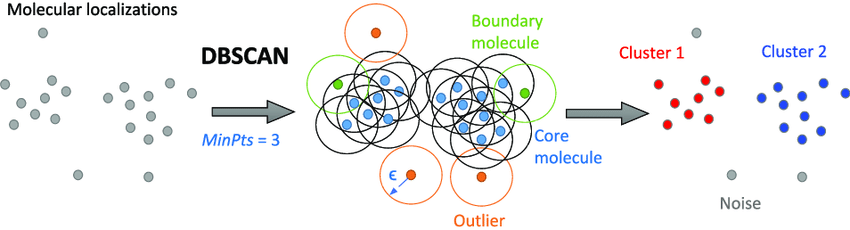
\includegraphics[width=0.9\linewidth]{png/An-Example-Illustrating-the-Density-Based-DBSCAN-Clustering-Method-Applied-to-SMLM-Data.png}
    \caption{An Example Illustrating the Density-Based DBSCAN Clustering Method Applied to SMLM Data}
    \label{fig:enter-label}
\end{figure}
Возникает 2 параметра: $\varepsilon$ и $m$. Других параметров не будет. От этих параметров и будет зависеть то, какой картина кластеризации получится. Также к преимуществам этого метода относится то, что он не задает заранее количество кластеров, в отличие, например, от k-means, причём количество кластеров будет зависеть от $\varepsilon$ и $m$. 

Как работает алгоритм: берётся произвольная точка, если она имеет плотную окрестность, то дальше рассматривается каждая точка этой плотной окрестности, и вокруг неё также строится $\varepsilon$-окрестность, и так пока не будет достигнута граница некоторого множества объектов. 

Хорошей аналогией может служить лес: один лес - это один кластер, через опушку, второй лес, - другой кластер, мы находимся в лесу. Смотрим, в нашей окрестности деревьев много, это значит, что мы в корневой точке находимся, и дальше мы идём, пока не выйдем на опушку леса, там мы окажемся в граничной точке - она уже не корневая, вокруг деревьев меньше. А где-то могут расти отдельно стоящие деревья - это шумовые выбросы. И вот так ходим по лесу, пока его весь не обойдём, и как только мы обошли весь лес, назовем его кластером. После чего случайно выбираем новое дерево и начинаем строить другой кластер.

Формализуем алгоритм в виде псевдокода:\\
\begin{tabularx}{\linewidth}{lX}
\textbf{вход:} выборка $X^l - \{x_1,...,x_l\}$; параметры $\varepsilon$ и $m$\\
\textbf{выход:} разбиение выборки на кластеры и шумовые выбросы;\\\hspace*{7mm}\hspace*{9mm}$U := X^l$ - не помеченные точки, $a := 0$\\
\textbf{пока} в выборке есть непомеченные точки, $U \neq \emptyset$:\\
\hspace*{7mm} взять случайную точку $x \in U$; \\
\hspace*{7mm} \textbf{если} $\abs{U_\varepsilon (x)} < m$ \textbf{то} \\
\hspace*{7mm}\hspace*{7mm} пометить $x$ как, возможно, шумовой;\\
\hspace*{7mm}\textbf{иначе} \\
\hspace*{7mm}\hspace*{7mm} создать новый кластер: $K:=U_\varepsilon (x); \; a:=a+1;$ \\
\hspace*{7mm}\hspace*{7mm} \textbf{для всех} $x' \in K$, не помеченных или шумовых \\
\hspace*{7mm}\hspace*{7mm}\hspace*{7mm} \textbf{если} $\abs{U_\varepsilon (x')} \geq m$,  \textbf{то} $K := K \cup U_\varepsilon (x')$; \\
\hspace*{7mm}\hspace*{7mm}\hspace*{7mm} \textbf{иначе} поментить $x'$ как граничный кластера $K$;\\
\hspace*{7mm}\hspace*{7mm} $a_j := a$ для всех $x_i \in K$;\\
\hspace*{7mm}\hspace*{7mm} $U := U \textbackslash K$;\\
\vspace{5mm}
\end{tabularx}

В таком виде алгоритм обладает следующими \textbf{свойствами}:
\begin{itemize}
    \item быстрая кластеризация больших данных: \\$O(l^2)$ в худшем случае, \\ $O(l \mathrm{ln} l)$ при эффективной реализации $U_\varepsilon (x)$;
    \item кластеры произвольной формы
    \item деление объектов на корневые, граничные, шумовые.
\end{itemize}

При этом важно понимать, что граничные объекты не выстраивают в точности границу каждого кластера. Практически это означает, что не стоит всерьез рассматривать граничные объекты, в отличие от шумовых, которые действительно можно в дальнейшем анализировать.

\subsection{Примечание о HDBSCAN} 
От гиперпараметра $\varepsilon$ можно избавиться, используя дивизивную кластеризацию. Такая модификация называется HDBSCAN. Его суть проста: необходимо построить дендрограмму, где по $Оу$ будет отложен $\varepsilon$ (на рис.\ref{fig:hdbdendro} снизу distance). Так мы сможем явно видеть вложенные кластеры. Алгоритм затем сам вычисляет оптимальное количество кластеров на основе метрики "стабильности кластеров".

\begin{figure}[h!]
    \centering
    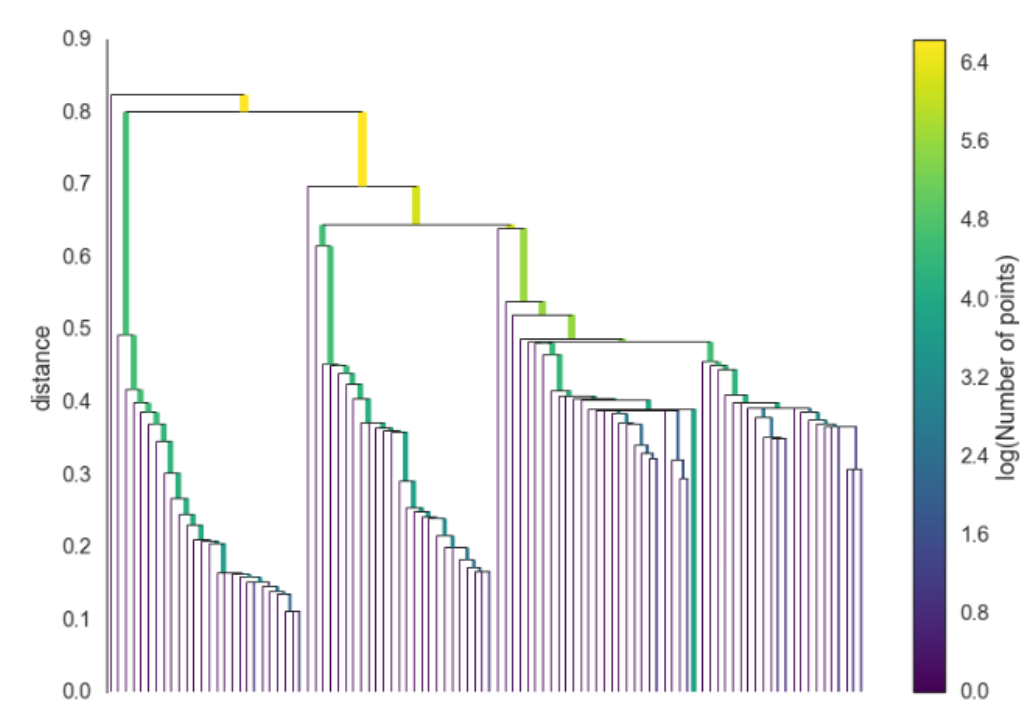
\includegraphics[width=0.6\linewidth]{png/hdbscan_dendrogramm.png}
    \caption{К примечанию о HDBSCAN}
    \label{fig:hdbdendro}
\end{figure}
\subsection{Задачи}
\textbf{Задача 1.}

\textbf{Условие.} Применить DBSCAN для выборки из таблицы с $m=4,\;\varepsilon=1.9$. Метрика евклидова.

\begin{center}
\begin{tabular}{ |c|c|c| } 
 \hline
 P1(3,7) & P5(7,3) & P9(3,3) \\ 
 P2(4,6) & P6(6,2) & P10(2,6) \\ 
 P3(5,5) & P7(7,2) & P11(3,5) \\ 
 P4(6,4) & P8(8,4) & P12(2,4) \\ 
 \hline
\end{tabular}
\end{center}

\textbf{Решение.}
Запишем матрицу, составленную из соответственных расстояний между точками выборки:
\begin{center}
\begin{tabular}{ |c|c|c|c|c|c|c|c|c|c|c|c|c|} 
 \hline
dot & P1 & P2 & P3 & P4 & P5 & P6 & P7 & P8 & P9 & P10 & P11 & P12 \\ \hline
P1 & 0 &  &  &  &  &  &  &  &  &  &  &   \\ \hline
P2 & 1.41 & 0 &  &  &  &  &  &  &  &  &  &   \\ \hline
P3 & 2.83 & 1.41 & 0 &  &  &  &  &  &  &  &  &   \\ \hline
P4 & 4.24 & 2.83 & 1.41 & 0 &  &  &  &  &  &  &  &   \\ \hline
P5 & 5.66 & 4.24 & 2.83 & 1.41 & 0 &  &  &  &  &  &  &   \\ \hline
P6 & 5.83 & 4.47 & 3.16 & 2.00 & 1.41 & 0 &  &  &  &  &  &   \\ \hline
P7 & 6.40 & 5.00 & 3.61 & 2.24 & 1.00 & 1.00 & 0 &  &  &  &  &   \\ \hline
P8 & 5.83 & 4.47 & 3.16 & 2.00 & 1.41 & 2.83 & 2.24 & 0 &  &  &  &   \\ \hline
P9 & 4.00 & 3.16 & 2.83 & 3.16 & 4.00 & 3.16 & 4.12 & 5.10 & 0 &  &  &   \\ \hline
P10& 1.41 & 2.00 & 3.16 & 4.47 & 5.83 & 5.83 & 5.66 & 6.40 & 6.32 & 0 &  &   \\ \hline
P11& 2.00 & 1.41 & 2.00 & 3.16 & 4.47 & 4.24 & 5.00 & 5.10 & 2.00 & 1.41 & 0 &   \\ \hline
P12& 2.83 & 3.16 & 4.00 & 5.10 & 4.47 & 5.39 & 6.00 & 1.41 & 2.00 & 2.00 & 1.41 & 0  \\ \hline
\end{tabular}
\end{center}
Сравнивая значения в каждом столбце матрицы с $\varepsilon$ и отбирая те, что меньше этого значения, находим окрестности каждой точки.

\begin{center}
\begin{tabular}{ |c|c| } 
 \hline
 точка & окрестность \\\hline
 P1 & P2, P10\\ 
 P2 & P1, P3, P11\\ 
 P3 & P2, P4\\ 
 P4 & P3, P5\\
 P5 & P4, P6, P7, P8\\
 P6 & P5, P7\\
 P7 & P5, P6\\
 P8 & P5\\
 P9 & P12\\
 P10 & P1, P11\\
 P11 & P2, P10, P12\\
 P12 & P9, P11\\
 \hline
\end{tabular}
\end{center}

Если в окрестности больше $m=4$ точек (включая ее саму), то отнесем эту точку к корневой, иначе - к шумовой.

\begin{center}
\begin{tabular}{ |c|c| } 
 \hline
 точка & тип \\\hline
 P1 & шум\\ 
 P2 & корневая\\ 
 P3 & шум\\ 
 P4 & шум\\
 P5 & корневая\\
 P6 & шум\\
 P7 & шум\\
 P8 & шум\\
 P9 & шум\\
 P10 & шум\\
 P11 & корневая\\
 P12 & шум\\
 \hline
\end{tabular}
\end{center}

Уточним классификацию, учтя граничные точки, т.е. точки, лежащие в окрестности корневых, но при этом не являющимися корневыми:
\begin{center}
\begin{tabular}{ |c|c| } 
 \hline
 точка & тип \\\hline
 P1 & граничная\\ 
 P2 & корневая\\ 
 P3 & граничная\\ 
 P4 & граничная\\
 P5 & корневая\\
 P6 & граничная\\
 P7 & граничная\\
 P8 & граничная\\
 P9 & шум\\
 P10 & граничная\\
 P11 & корневая\\
 P12 & граничная\\
 \hline
\end{tabular}
\end{center}

К первому кластеру отнесем окрестность корневой точки 2, причем в ее окрестности находится еще одна корневая точка 11, так что отнесем и ее окрестность к первому кластеру. Ко второму кластеру отнесем корневую точку 5 и ее окрестность. Осталась лишь одна точка P9, которая не относится ни к какому кластеру и является шумовой.
\begin{figure}[h!]
    \centering
    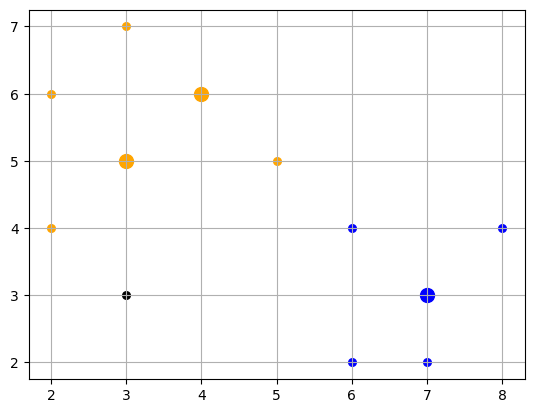
\includegraphics[width=0.7\linewidth]{png/task1dbs_plot.png}
    \caption{Кластеризация в задаче 1}
    \label{fig:task1dbs}
\end{figure}

\begin{minipage}{.5\textwidth}
\textbf{Задача 2.}\\
\textbf{Условие.}
  Сравните результаты кластеризации с помощью k-means и с помощью DBSCAN и объясните их.\\
\textbf{Решение.}
Объяснение различий:
\begin{itemize}
\item \textit{Форма кластера}:
K-средние: стремится найти сферические или выпуклые кластеры. Предполагается, что кластеры изотропны (однородны во всех направлениях) и имеют схожий размер.
DBSCAN: может обнаруживать кластеры произвольной формы и размера. Не делает предположений о форме кластеров.
\item \textit{Обработка шума}:
K-средние: плохо справляется с шумом. Точки шума могут быть назначены кластерам, что может повлиять на центры кластеров.
DBSCAN: может идентифицировать и маркировать точки шума, которые не назначены ни одному кластеру.
\end{itemize}
\end{minipage}% This must go next to `\end{minipage}`
\begin{minipage}{.4\textwidth}
      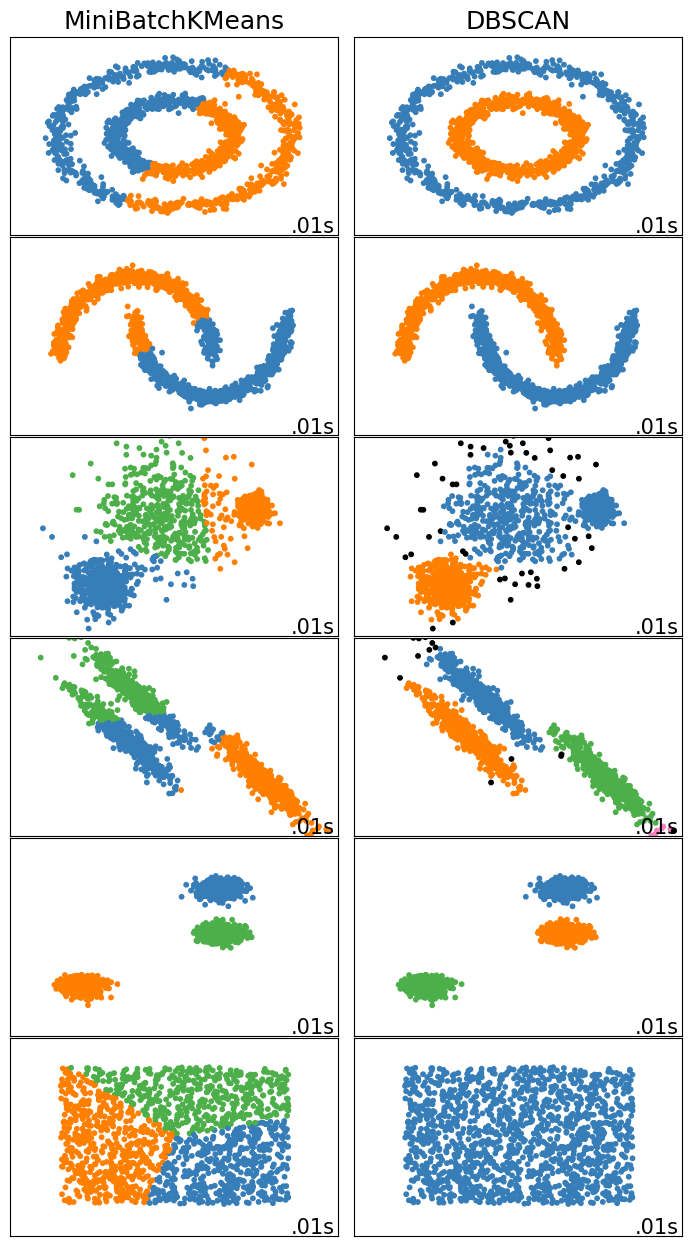
\includegraphics[width=0.95\linewidth]{png/task2dbs_plot.png}
\end{minipage}
\begin{itemize}
\item \textit{Плотность кластера}:
K-средние: не учитывает плотность точек. Каждый кластер представлен центроидом.
DBSCAN: учитывает плотность точек. Кластеры формируются на основе плотности точек в окрестности.
\item \textit{Чувствительность параметров}:
K-средние: требует предварительного указания количества кластеров (K), так что, если если заранее указать 3 кластера, то алгоритм и найдет три кластера, даже если он всего один, как на последней паре картинок.
\end{itemize}

\textbf{Задача 3.}\\
\textbf{Предисловие.}
При решении задачи 1 использовалась матрица, состоящая из расстояний между парами точек (\textit{матрица смежности}). Понятием, противоположным расстоянию, является понятие сходства между объектами. Неотрицательная вещественная функция $S(x_i,x_j) = S_{ij}$ называется \textit{мерой сходства}, если:
\begin{itemize}
    \item $0 \leq S(x_i,x_j) < 1$, для $x_i \neq x_j$
    \item $S(x_i,x_j)=1$
    \item $S(x_i,x_j)=S(x_j,x_i)$
\end{itemize}
Пары значений мер сходства можно объединить в \textit{матрицу сходства} $S$, симметричную и единичной диагональю.
\textbf{Условие.}
Применить DBSCAN с пороговым значением \textit{меры сходства} 0.8 и $m = 2$ и заданной матрицей сходства между точками выборки:

\begin{center}
\begin{tabular}{ |c|c|c|c|c|c|} 
 \hline
dot & P1 & P2 & P3 & P4 & P5  \\ \hline
P1 & 1.0 &  &  &  &     \\ \hline
P2 & 0.10 & 1.0 &  &  &  \\ \hline
P3 & 0.41 & 0.64& 1.0 &  & \\ \hline
P4 & 0.55 & 0.47 & 0.44 & 1.0 & \\ \hline
P5 & 0.35 & 0.98 & 0.85 & 0.76 & 1.0 \\ \hline
\end{tabular}
\end{center}

Сравнивая значения в каждом столбце матрицы с $\varepsilon$ и выбирая те точки, для которых значение сходства выше, чем порог, формируем окрестности всех точек.

\begin{center}
\begin{tabular}{ |c|c| } 
 \hline
 точка & окрестность \\\hline
 P1 & -\\ 
 P2 & P5\\ 
 P3 & P5\\ 
 P4 & -\\
 P5 & P2, P3\\
 \hline
\end{tabular}
\end{center}

Если в окрестности больше $m=2$ точек (включая ее саму), то отнесем эту точку к корневой, иначе - к шумовой.

\begin{center}
\begin{tabular}{ |c|c| } 
 \hline
 точка & тип \\\hline
 P1 & шум\\ 
 P2 & корневая\\ 
 P3 & корневая\\ 
 P4 & шум\\
 P5 & корневая\\
 \hline
\end{tabular}
\end{center}

Уточнение классификации, путем учитывания граничных точек, т.е. точек, лежащие в окрестности корневых, но при этом не являющимися корневыми, ничего не дает, т.к. в окрестности точек, определенных как шумовые вообще нет других точек, так что они действительно являются шумом.

К первому кластеру отнесем окрестность корневой точки P2, причем в ее окрестности находятся еще краевая точка P5, так что отнесем ее к этому же кластеру. В окрестности точки P5 помимо уже классифицированной P2 находится еще корневая точка P3, которую также отнесем к первому кластеру. Остальные точки классифицированы как шумовые. Таким образом в данной задаче всего один кластер, состоящий из точек P2, P3, P5.

\section{Простые эвристические методы частичного обучения}
\subsection{Постановка задачи}
Существует привычная нам задача классификации. Мы имеем $X$ --- множество объектов с известными признаками и $Y$ --- пространство классов. Есть неизвестная функция $X \longrightarrow Y$, сопоставляющая каждому обьекту его класс. Имеется обучающая выборка $\{x_1, x_2, ...\} \subset X$ и соответствующие им известные классы $\{y_1, y_2, ...\} \subset Y$. Задача классификации сводится к построению классификатора --- некой аппроксимации неизвестной функции $X \longrightarrow Y$. \\

С другой стороны существует задача кластеризации. Мы все также имеем $X$ --- множество объектов. И хотим аппроксимировать функцию $X \longrightarrow Y$. Но на этот раз у нас нет обучающей выборки, зато есть функция расстояния между объектами $\rho: X\times X \longrightarrow \mathbb{R}$. И в этом случае кластеризующая функция строится не на основе обучающей выборки, а так чтобы расстояние между объектами одного кластера было мало, а расстояние между объектами разных кластеров было велико. \\

Первый случай называется обучение с учителем,а кластеризация называется обучением без учителя. Где-то по середине между этими задачами находится задача частичного обучения. В этом случае у нас все также есть множество обьектов из $X$ и (возможно) функция $\rho$. При этом только для некоторой доли имеющихся обьектов известна классовая принадлежность. Иначе говоря обучающая выборка размечена \textbf{частично}. \\

Приведем пример (Рис. 1). Допустим известные обьекты в пространстве признаков имеют вид в виде двух бананов. И нам известна принадлежность только двух точек. В таком случае чистая задача кластеризации обучит классификатор только по двум точкам, который будет иметь сомнительное качество на всех остальных данных. При это частичное обучение могло бы учесть явную кластеризацию данных и дать значительно лучшую классификацию.\\

\begin{center}
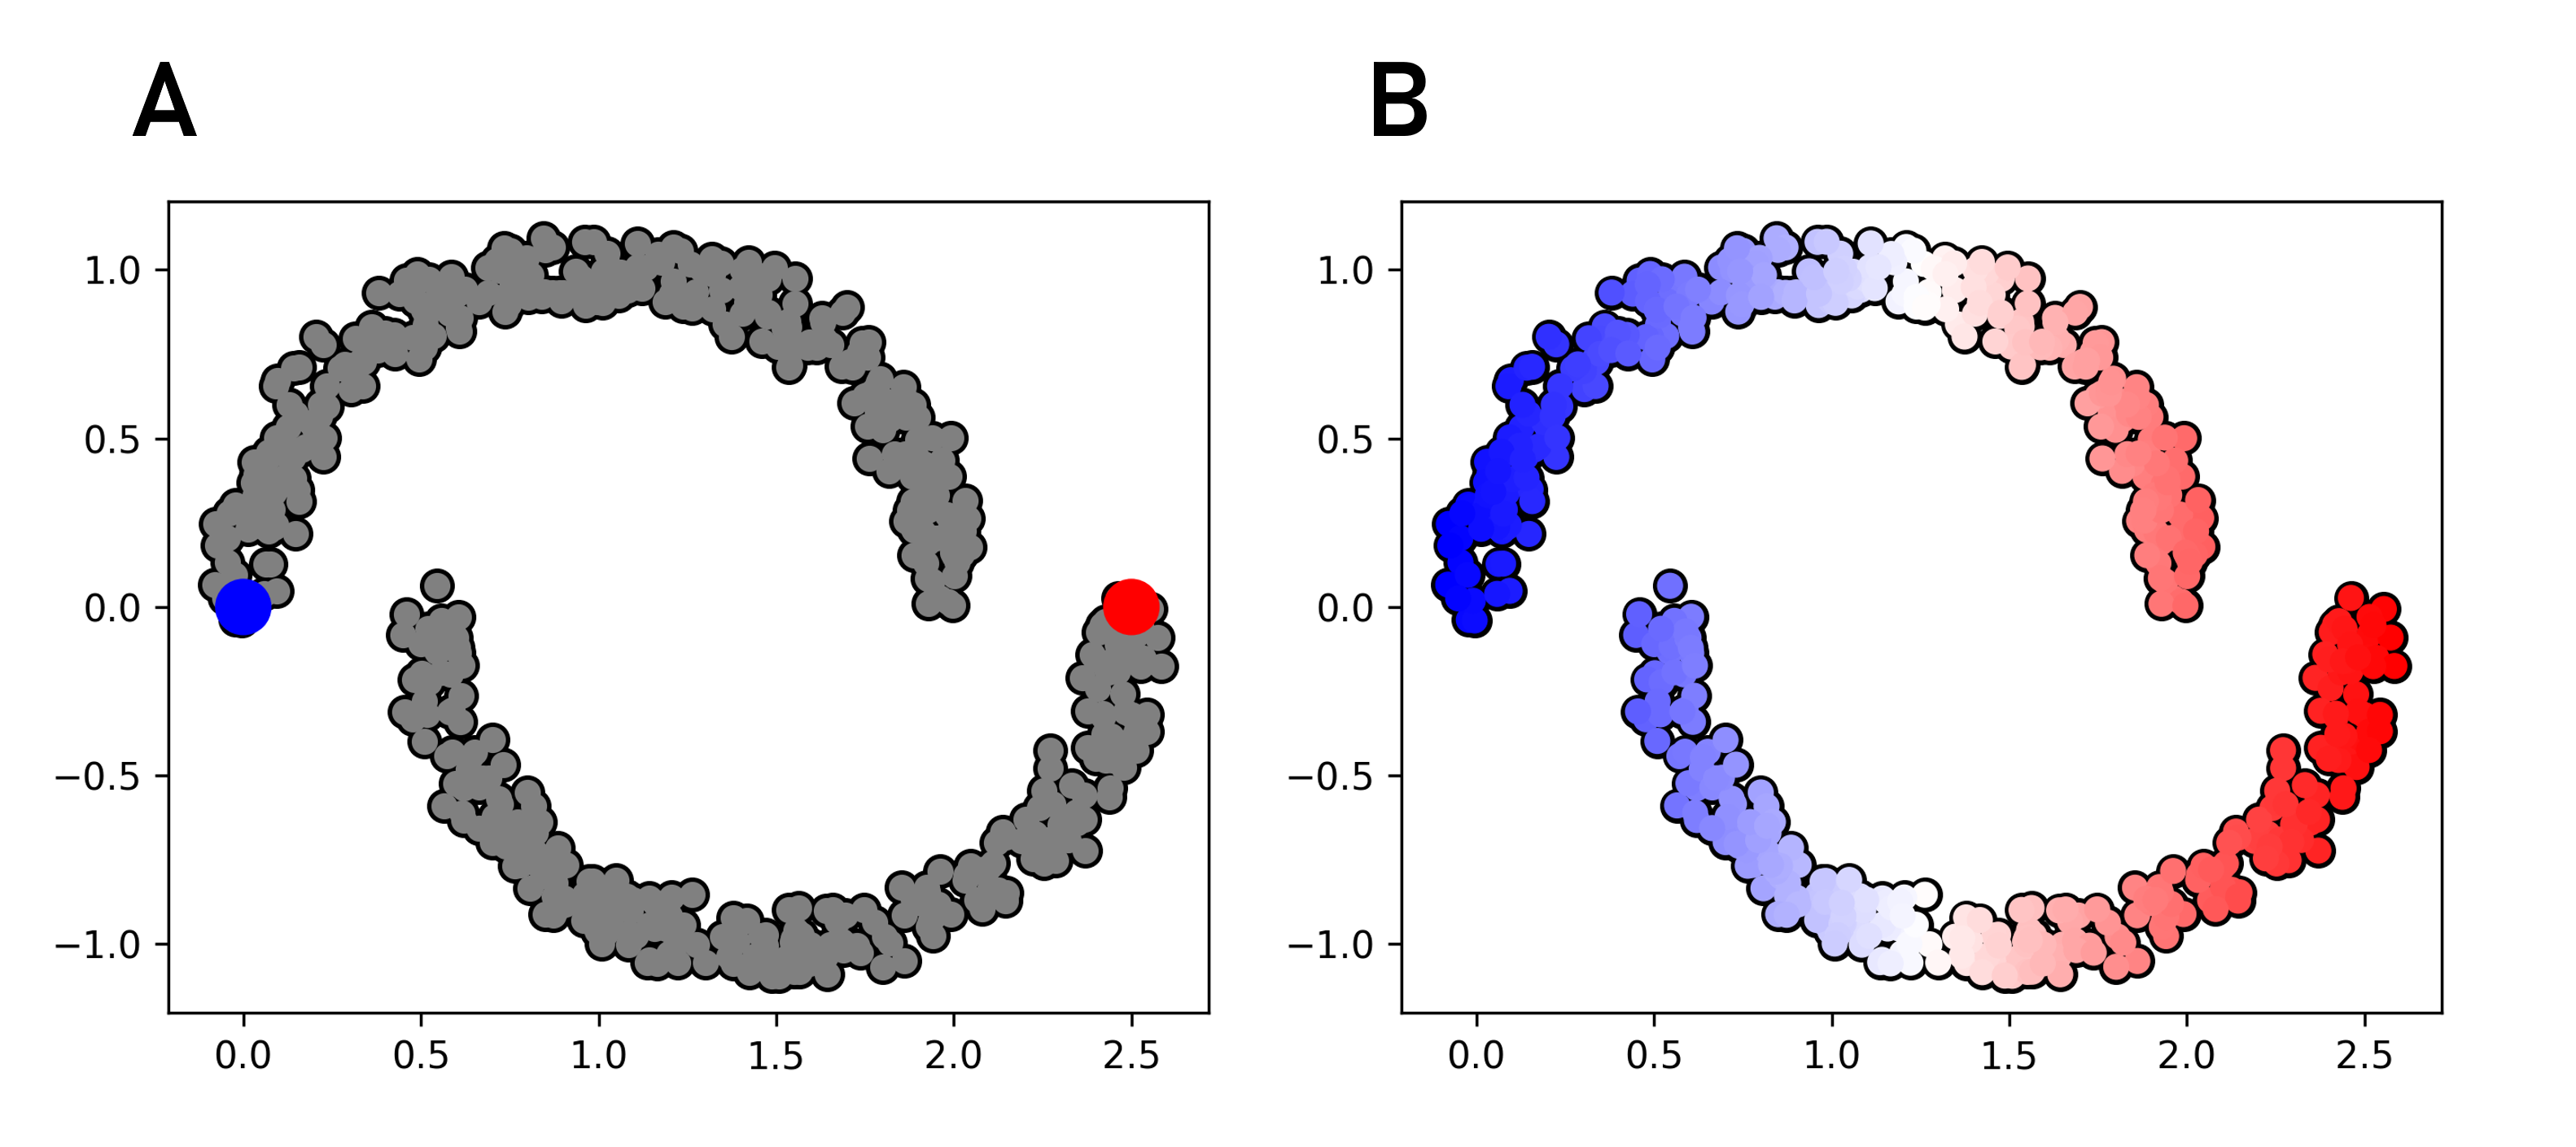
\includegraphics[width=1.0\textwidth]{picture_1.png}
\textbf{Рисунок 1.} (\textbf{A}) Пример частично размеченных данных. (\textbf{B}) Классификация обученная на размеченных данных не учитывает кластерную структуру неразмеченных. 
\end{center}

Однако частичное обучение не может сводиться только к кластеризации, представьте теперь, что мы знаем классы уже трех точек на выборке из двух бананов (Рис. 2). В таком случае кластеризация дала бы предсказание которое не может соотноситься с известными классами всех трех точек. Таким образом задача частичного обучения действительно находится посередине между классификацией и кластеризацией, но не является ни тем, ни другим. \\
\begin{center}
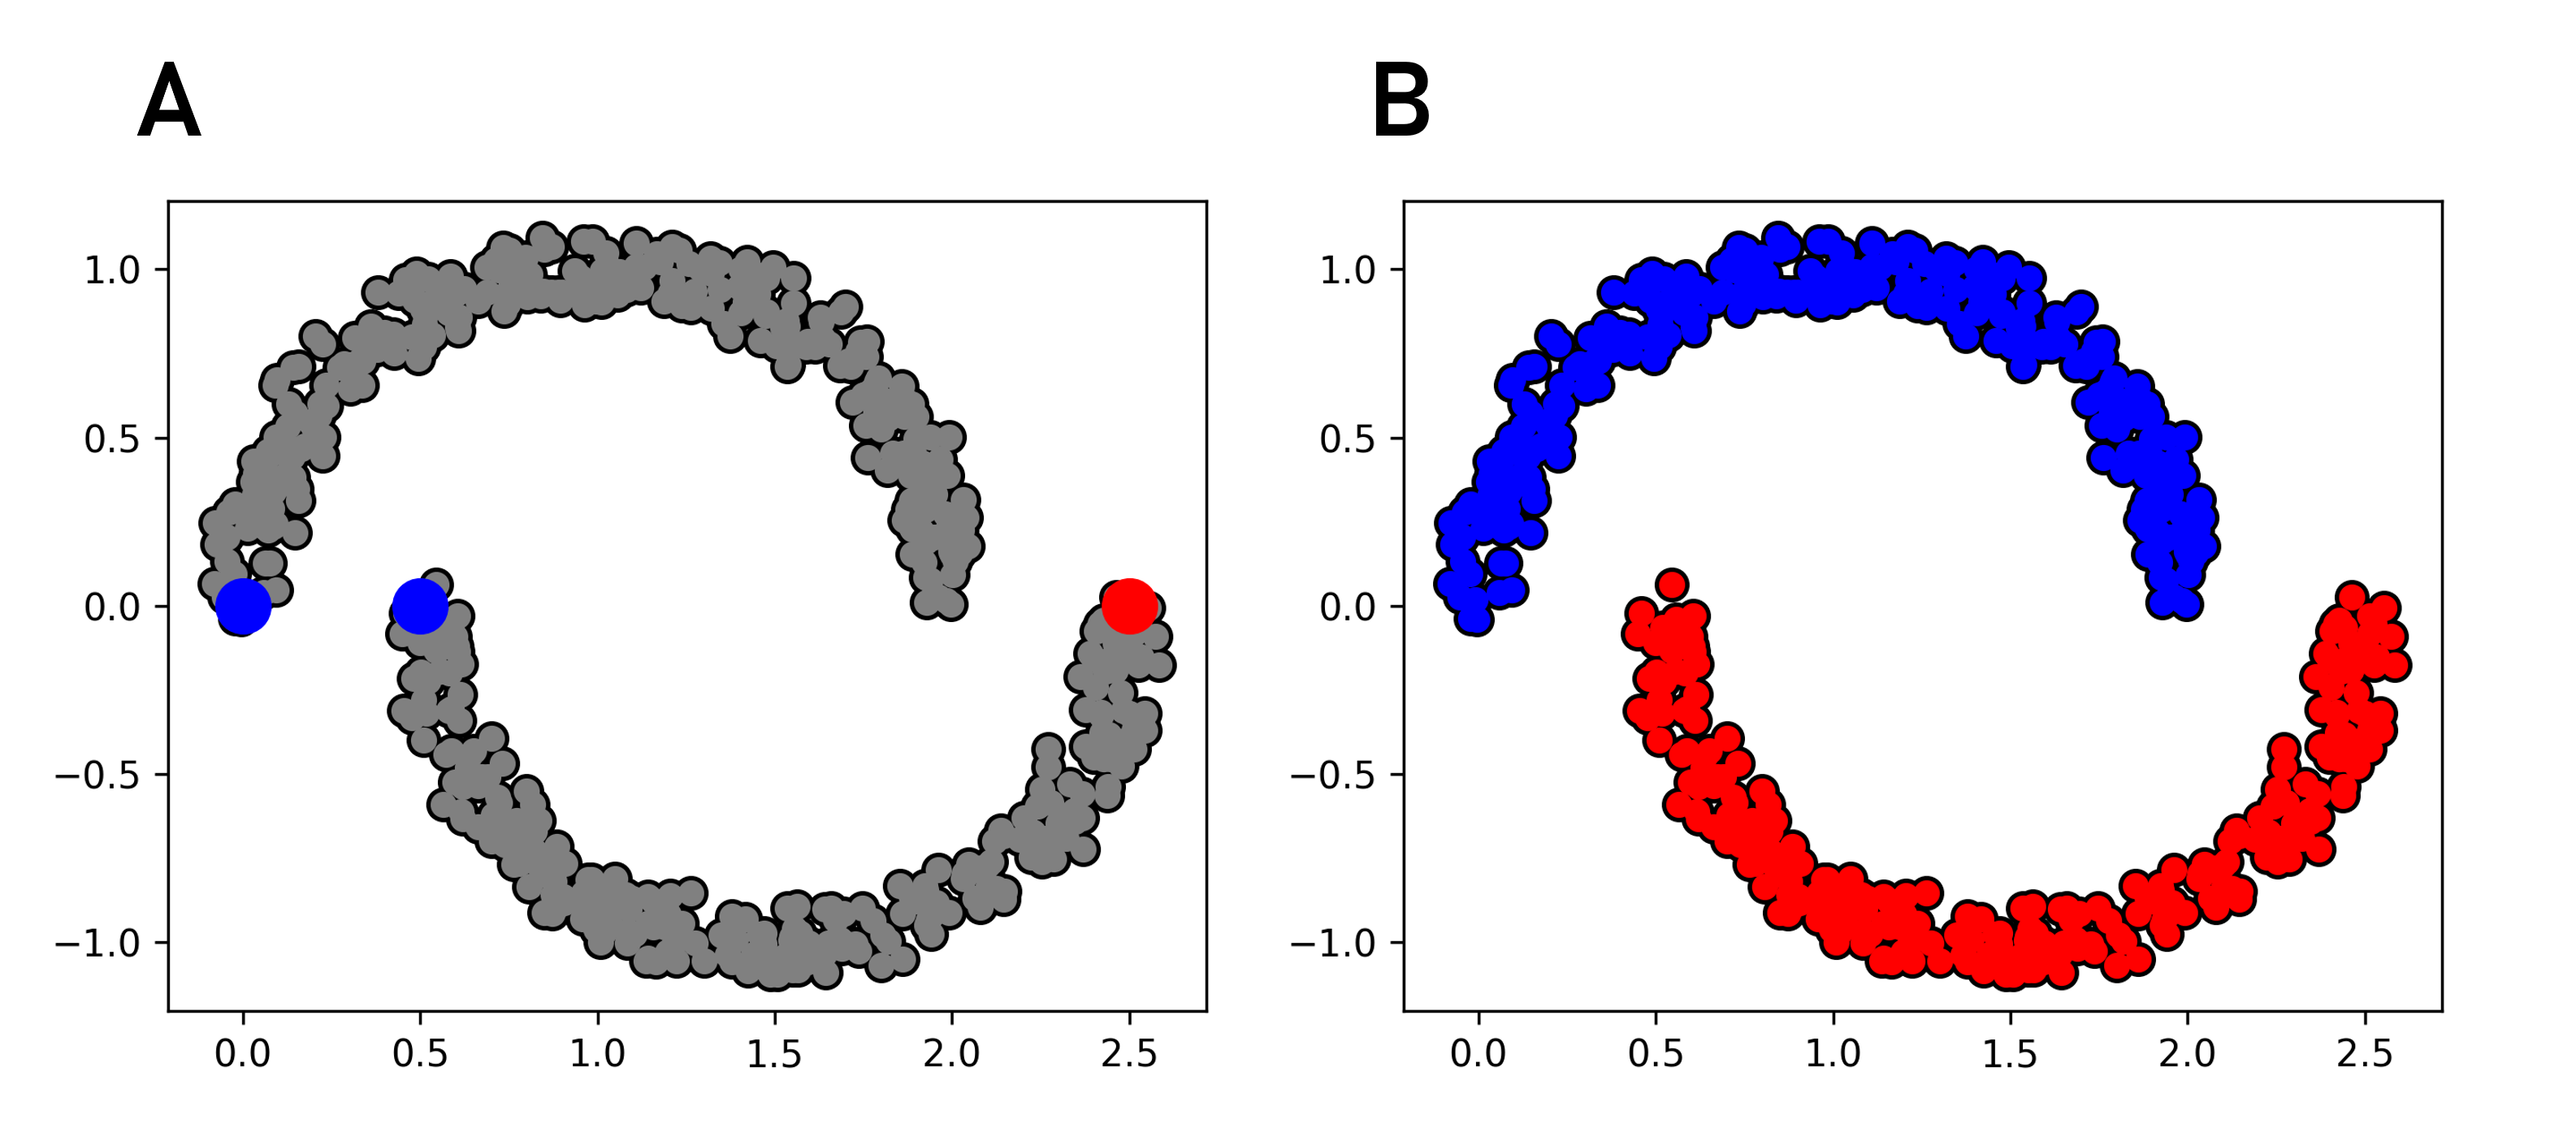
\includegraphics[width=1.0\textwidth]{picture_2.png}
\textbf{Рисунок 2.} (\textbf{A}) Пример частично размеченных данных. (\textbf{B}) Кластеризация не учитывает классовую принадлежность размеченных данных. 
\end{center}

Приведем пример: программист решил сделать классификатор для фотографий котиков и собачек, для этого он скачал по миллиону фотографий и тех и других. Однако, ему хватило сил подписать котик это или собачка только для 1000 фотографий. Классификация не может быть построена только по 1000 фотографиям --- мало данных, а кластеризация может разбить фотографии неизвестным образом --- по цвету фона, по размеру животного. И только частичное обучение может помочь ленивому программисту.
\subsection{Self-training}
Каким же образом можно реализовать частичное обучение? Рассмотрим подход, который называется self-training (само-обучение). Вернемся к датасету с бананами в котором известны классы двух точек. Как было сказано ранее построение классификатора по двум точкам тут не поможет. Однако допустим, что мы все же построили классификатор по двум точкам, к примеру логистическую регрессию. Вспомним что многие методы классификации могут оценивать свою уверенность в предсказании. Тогда для некоторых точек с наибольшей уверенностью классификации (скажем 5\% самых уверенных) предсказание  классификации может оказаться вполне верным. Давайте же дополним обучающую выборку классификатора этими точками. На второй итерации нашего подхода мы обучим классификатор уже по дополненной обучающей выборке. Выполнив предсказание для остальных данных, выберем еще раз 5\% ранее неразмеченных точек с наибольшей уверенностью и пополним ими обучающую выборку. Будем повторять такие итерации пока не классифицируем все точки в нашем датасета. Как мы видим, результат такого подхода заметно лучше, чем у классификации по двум исходным точкам. 
\begin{center}
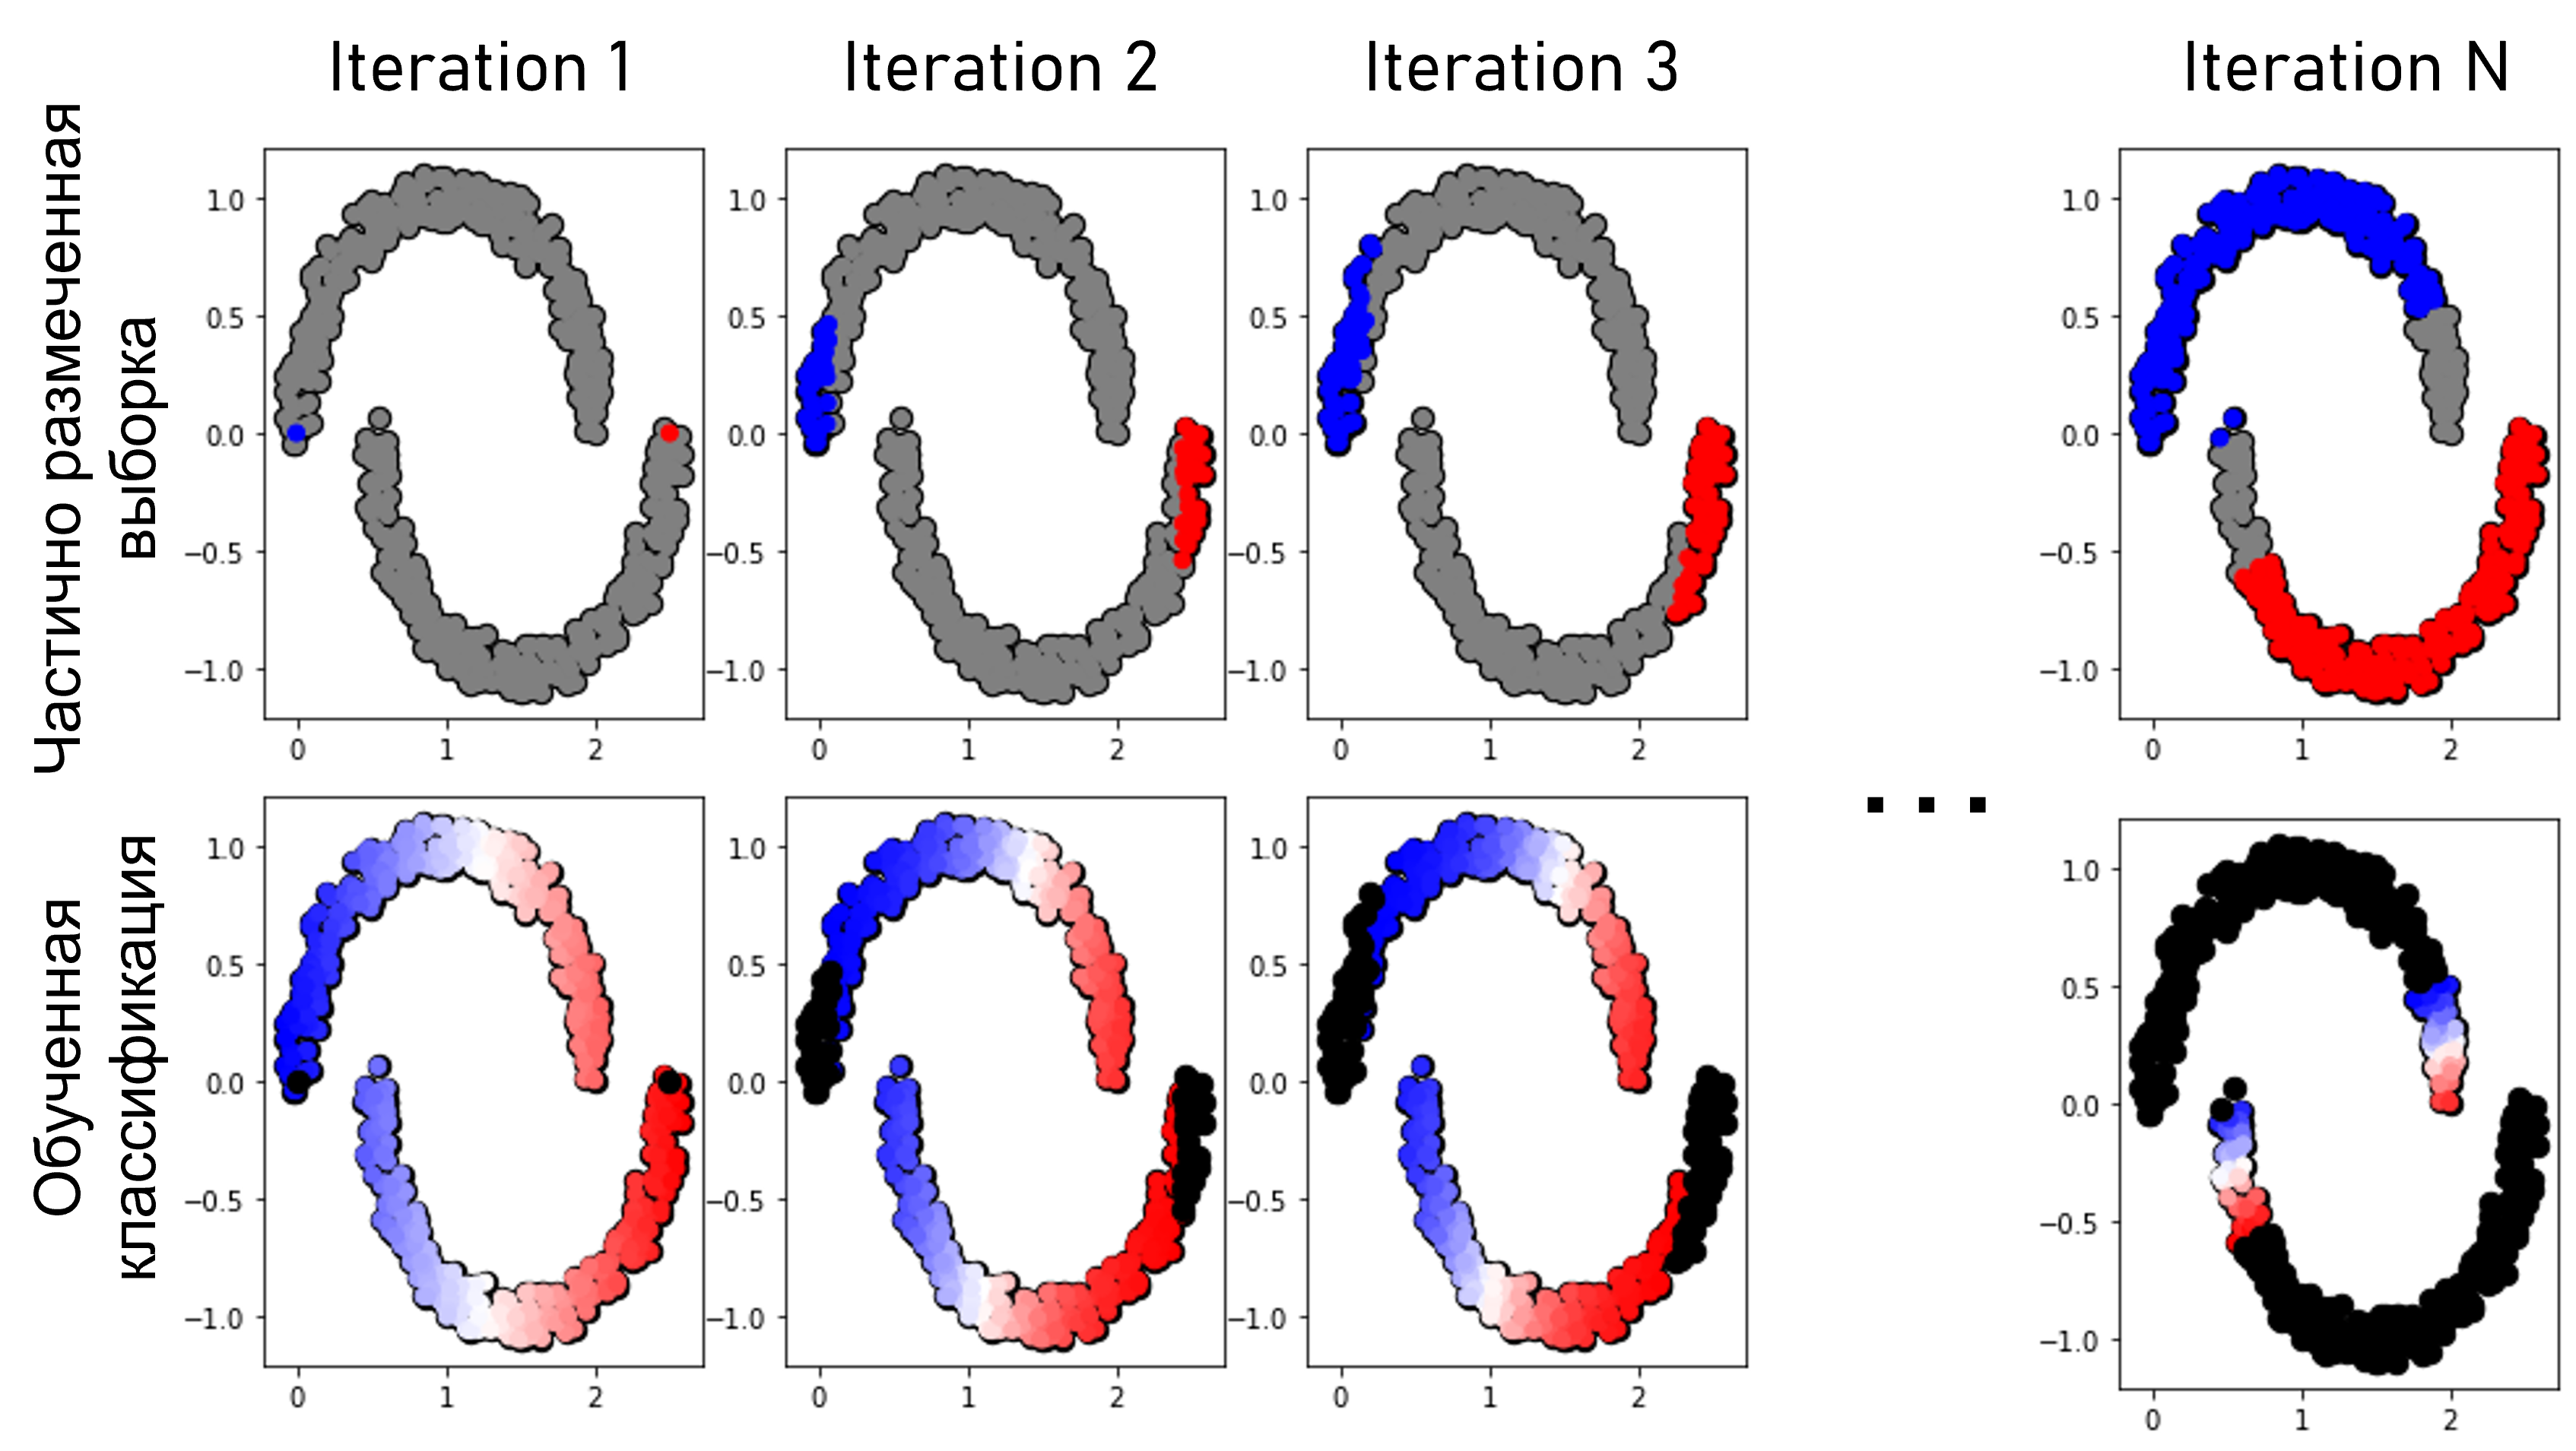
\includegraphics[width=1.0\textwidth]{picture_3.png}
\textbf{Рисунок 3.} Пример работы итераций self-training. 
\end{center}
Оформим описанный процесс более математизировано. Пусть мы строим функцию $a: X \longrightarrow Y$. Пусть у нас есть метод обучения функции $\mu: Z \longrightarrow a$ который принимает на вход размеченную часть выборки $Z \subset X$. Допустим функция $a$ имеет вид
\begin{equation*}
    a(x) = \arg \max_{y \subset Y}\Gamma_y(x)
\end{equation*}
где $\Gamma_y(x)$ это некоторые (к примеру) линейные функции от $x \subset X$ которые обучаются так, чтобы быть большими, если $x$ принадлежит классу $y$ и маленькими в противном случае. В таком случае уверенность классификации в принадлежности элемента $x$ к классу $y_1$ (отступ):
\begin{equation*}
    M_1(x) = \Gamma(x) - \max_{y \subset Y\backslash y_1}\Gamma_{y_1}(x) 
\end{equation*}
Пусть $Z$ это размеченная часть обучающей выборки. Тогда алгоритм выглядит так:
\begin{enumerate}
  \item $a = \mu(Z)$ --- обучить классификатор на размеченной выборке
  \item $\Delta := \{x \subset X\backslash Z \;|\; M(x) \geq M_0 \}$ --- выбрать несколько точек из неразмеченной части выборки которые наиболее уверенно классифицируются. 
  \item $Z := Z\cup\Delta$ --- дополнить размеченную выборку
  \item Если не все элементы выборки размечены, вернуться в начало.
\end{enumerate}
\subsection{Сo-training}
Рассмотрим более узкий кейс, допустим у нас есть не один, а целых два метода обучения классификации $\mu_1, \mu_2$, которые принципиально отличаются друг от друга, например имеют разные парадигмы обучения, и/или используют разные признаки обьектов, и/или имеют разную стартовую выборку. В таком случае мы можем получить преимущество в частичном обучении заставив их учить друг друга по следующему алгоритму:
\begin{enumerate}
  \item $a_1 = \mu_1(Z_1)$\\
  $a_2 = \mu_2(Z_2)$ --- два метода обучают классификаторы на своих размеченных выборках. 
  \item $\Delta_1 := \{x \subset X\backslash Z_1\backslash Z_2 \;|\; M_1(x) \geq M_{01} \}$ --- метод 1 размечает неразмеченные точки, в которых он уверен.\\
  $\Delta_2 := \{x \subset X\backslash Z_1\backslash Z_2 \;|\; M_2(x) \geq M_{02} \}$ --- метод 2 делает тоже самое.
  \item $Z_1 := Z_1\cup\Delta_2$ --- метод 2 дополняет обучающую выборку метода 1 \\
  $Z_2 := Z_2\cup\Delta_1$ --- метод 1 дополняет обучающую выборку метода 2
  \item Если не все элементы выборки размечены, вернуться в начало.
\end{enumerate}
\subsection{Сo-learning}
Идем еще дальше, допустим у нас теперь есть набор методов $\mu_i$ отличающиеся чем-то. Допустим что все эти методы обучились на одной выборке $Z$ и произвели классификаторы $a_i$. Давайте соберем из множества классификаторов $a_i$ один классификатор-мегазорд:
\begin{equation*}
    a(x) = \arg \max_{y \subset Y}\Gamma_y(x)
\end{equation*}
Где на этот раз функции $\Gamma$ определяются как:
\begin{equation*}
    \Gamma_y(x) = \sum_{i = 1}^{I}[a_i(x) = y]
\end{equation*}
Выражение в квадратных скобках равно 1 когда написанное в них верно, и равно 0 в противных случаях. Иначе говоря, классификаторы $a_i$ голосуют за принадлежность к классам, и демократически выбирают к кому классу отнести каждый из обьектов. Далее на основе такого обьединенного классификатора строится Self-training описанный выше. 
\subsection{Задачи}
\subsection*{Задача 1}
Возможно ли при помощи self-training эффективно классифицировать точки частично размеченной выборки представленной ниже:
\begin{center}
\includegraphics[width=0.5\textwidth]{picture_5.png}
\end{center}
\textit{\textbf{Решение:} Конечно можно! Для этого нужно построить self-training на основе классификатора который может делать разделяющую поверхность в виде окружности, например классификаторы восстанавливающие плотность или логистическая регрессия с добавлением квадратичных признаков}
\subsection*{Задача 2}
Два подхода частичного обучения применяются для классификации обьектов частичной выборки представленной ниже.
\begin{center}
\includegraphics[width=0.5\textwidth]{picture_4.png}
\end{center}
Первый подход это self-training на основе логичтической регрессии, которая видит только первый признак. Второй подход это co-training на основе двух логистических регрессий, таких что первая видит первый признак, а вторая второй. Какой алгоритм приведет к лучшей классификации точек и почему?\\

\textit{\textbf{Решение:} self-training видящий только первый признак веротянее всего идеально классифицирует точки, так как по этому признаку кластеры разделены и практически не пересекаются. В случае co-training классификатор использующий второй признак видит кластеры пересекающимися и почти наверняка наделает ошибок при классификации}
\subsection*{Задача 3}
Алгоритм co-training построенный на основе трех классификаторов классифицирует точки представленной ниже выборки. На последней итерации работы алгоритма осталась лишь одна неклассифицированная точка. На этот момент классификаторы имеют разделяющие линии представленные на картинке. К какому кластеру будет отнесена оставшаяся точка?
\begin{center}
\includegraphics[width=0.5\textwidth]{picture_6.png}
\end{center}
\textit{\textbf{Решение:} Судя по разделяющим линиям два классификатора проголосую за красный кластер, и только один за синий, в итоге точка будет отнесена к красному кластеру.}

\subsection*{Алгоритм Ланса-Уильямса} % Aleksandrov Nikta

Пусть $X = \{\{x_1\},..., \{x_l\}\}$ - исходная выборка, $l$ - количество её элементов, необходимо объединить объекты выборки в кластере на основе расстояний между ними. Алгоритм инициализируется таким образом, что каждый объект выборки считается отдельным кластером, затем происходит итеративное слияние кластеров друг с другом. Критерием, по которому кластеры объединяются, является расстояние между ними. %$R(\{x_i\}, \{x_j\}) = \rho (x_i, x_j)$.
Существует множество способов выбора метрики расстояния между кластерами, однако большинство классических метрик можно обобщить, используя формулу Ланса-Уильямса.\\
Пусть в процессе вычисления имеется набор кластеров $C_t,t \in \{1, \l\}$, $U, V$ - кластеры, которые были выбраны для слияния, $W = U \cup V$ , тогда для произвольного кластера $S \in C_t\ \cup \{W\} \textbackslash \{U, V\}$ расстояние $R_{WS}$ до кластера $W$ определяется по следующей формуле.

\begin{equation*}
        R_{WS} = \alpha_U \cdot R_{US} + \alpha_V \cdot R_{VS} + \beta \cdot R_{UV} + \gamma \cdot |R_{US} - R_{VS}|
\end{equation*}

где $R_{US}, R_{VS}, R_{UV}$ - расстояния между кластерами $U$ и $S$, $V$ и $S$, $U$ и $V$ соответственно, $\alpha_U, \alpha_V, \beta, \gamma$ - некоторые действительные коэффициенты. Рассмотрим стандартные способы задания метрики расстояния между множествами и покажем, какие значения коэффициентов соответствуют им:

\begin{itemize}
    \item Расстояние до ближайшего соседа: $R^{\text{б}}_{WS} = \underset{w \in W, s \in S}{min}
  \rho (w, s)$; $\alpha_U = \alpha_V = \frac{1}{2}, \beta = 0, \gamma = - \frac{1}{2}$
    \item Расстояние до наиболее удалённого соседа: $R^{\text{д}}_{WS} = \underset{w \in W, s \in S}{max} \rho (w, s)$; $\alpha_U = \alpha_V = \frac{1}{2}, \beta = 0, \gamma = \frac{1}{2}$
    \item Среднее расстояние между элементами кластера: $R^{\text {с}}_{WS} = \frac{1}{|W||S|} \sum_{w \in W} \sum_{s \in S} \rho (w, s)$; $\alpha_U = \frac{|U|}{|W|}, \alpha_V = \frac{|V|}{|W|}, \beta = \gamma = 0$
    \item Расстояние между центрами: $R^{\text{ц}}_{WS} = \rho^2 \left( \sum_{w \in W} \frac{w}{|W|}, \sum_{s \in S} \frac{s}{|S|} \right)$; $\alpha_U = \frac{|U|}{|W|}, \alpha_V = \frac{|V|}{|W|}, \beta = \alpha_U \cdot \alpha_V, \gamma = 0$
    \item Расстояние Уорда: $R^{\text{у}}_{WS} = \frac{|S||W|}{|S|+|W|} \rho^2 \left( \sum_{w \in W} \frac{w}{|W|}, \sum_{s \in S} \frac{s}{|S|} \right)$; $\alpha_U = \frac{|S| + |U|}{|S|+|W|}, \alpha_V = \frac{|S|+|V|}{|S|+|W|}, \beta = \frac{-|S|}{|S|+|W|}, \gamma = 0$
\end{itemize}

Таким образом, данная метрика действительно является обобщением множества классических способов определения расстояния между кластерами. Ниже представлен псевдокод алгоритма Ланса-Уильямса.

\begin{algorithm}
\caption{Агломеративная кластеризация Ланса-Уильямса}\label{Lance–Williams}
\begin{algorithmic}
\State $t:=1$: $C_t = \{\{x_1\},...,\{x_l\}\}$
\ForEach {$s \in \mathcal S $}
\State найти в $C_{t - 1}$ пару кластеров $U, V$ с минимальным $R_{UV}$
\State $W = U \cup V;$
\State $C_t = C_{t - 1} \cup \{W\} \textbackslash \{U, V\};$
\ForEach {$S \in C_t$}
\State $R_{WS} = \alpha_U \cdot R_{US} + \alpha_V \cdot R_{VS} + \beta \cdot R_{UV} + \gamma \cdot |R_{US} - R_{VS}|$

\end{algorithmic}
\end{algorithm}

На выходе алгоритма получается кластер, состоящий из всех элементов исходной выборки, разделённый иерархически на подкластеры. Дальнейшей задачей является выделение основных подкластеров из данного набора кластеров для дальнейшей работы с ними. Это удобно сделать, используя дендрограмму - график, визуализирующий расстояние между кластерами, образующимися в процессе вычислений.

\begin{center}
\begin{figure}[H]
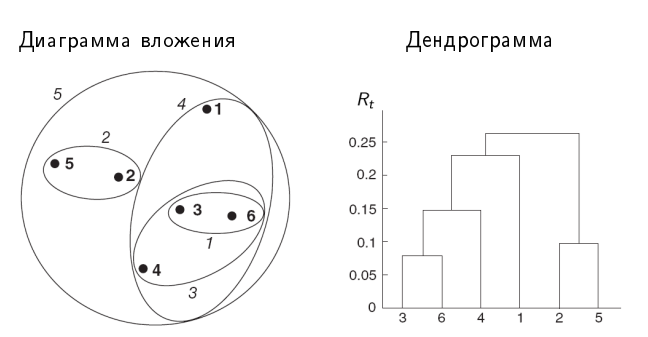
\includegraphics[width=14cm]{png/Dendrogramma.png}
\caption{Визуализация объектов кластеров и соответствующая им дендрограмма для алгоритма Ланса-Уильямса, в качестве расстояния используется расстояние Уорда}
\label{fig:Dendrogramma}
\end{figure}
\end{center}

На данной дендрограмме можно провести горизонтальную линию по уровню $R_0$, что и определит конечную структуру кластеров. Проще всего сделать это путём отсечения правого участка дендрограммы. На горизонтальной оси находится интервал максимальной длины $|R_{t+1} - R_t|$, в качестве результирующей кластеризации выдаётся множество кластеров $C_t$, их число $K = l - t + 1$. Для того, чтобы улучшить качество кластеризации, необходимо, чтобы метрика расстояния обладала определёнными свойствами.

\subsection*{Монотонность}

Функция расстояния $R$ обладает свойством монотонности, если при каждом слиянии расстояние между объединяемыми кластерами увеличивается: $R_2 \leq R_3 \leq...\leq R_l$. В таких случая дендрограмму можно построить без самопересечений, что в свою очередь позволяет выделить чёткую кластерную структуру. Существует достаточное условие монотонности функции расстояния:

\textbf{Теорема Миллигана.} Если выполняются следующие 3 условия, то кластеризация является монотонной
\begin{itemize}
    \item $\alpha_U \geq 0, \alpha_V \geq 0$;
    \item $\alpha_U + \alpha_V + \beta \geq 1;$
    \item $min \{{\alpha_U, \alpha_V}\} + \gamma \geq 0$
\end{itemize}

\subsection{Свойства растяжения и сжатия}

Фукнция расстояния $R$ обладает свойством растяжения, если при каждом слиянии расстояние от него до других кластеров увеличивается. Функция расстояния $R$ обладает свойством сжатия, если при каждом слиянии расстояние от него до других кластеров уменьшается. Растяжение способствует более чёткому отделению кластеров, однако при избыточно слишком большом растяжении некоторые кластеры находятся там, где их изначально не было. На практике используется гибкое расстояние, являющееся компромиссом между методами ближнего, дальнего соседа и среднего расстояния, регуляруется параметром $\beta$: $\alpha_U = \alpha_V = (1 - \beta)/2, \beta < 1$. При $\beta > 0$ расстояние является сжимающим, при $\beta < 0$ растягивающим. Более точный подбор $\beta$ проводится на основе анализа конкретной задачи. 

В целом, нельзя однозначно сказать, какой выбор коэффициентов даст лучший результат. Среди перечисленных расстояний наиболее стабильным принято считать расстояние Уорда. Однако для улучшения качества кластеризации рекомендуется исследовать алгоритм на точность при различных вариантах метрики. 

\subsection*{Задачи на данную тему}

\subsubsection*{Задача 1} 
Сгенерируйте 2 двухмерых гауссиана с единичными матрицами ковариации, но различными векторами средних. Используйте алгоритм Ланса-Уильямса для кластеризации получившихся наборов точек. Проведите вычисления для разных значений $|\Vec{\mu_1} - \Vec{\mu_2}|$, где $\Vec{\mu_1}$ - вектор среднего для первого гауссиана, $\Vec{\mu_2}$ - вектор среднего для второго гауссиана. Сравните полученные результаты с результатами, получаемыми с помощью алгоритма восстановления плотности вероятности. 

\subsubsection*{Задача 2} 
Возьмите статистику по среднему баллу по базовым кафедральным предметам, количество времени, проводимого на кафедре и на работе/стажировке, а также зарплату для всех студентов вашего потока. Используйте алгоритм Ланса-Уильямса и оцените, насколько часто студенты одной кафедры оказываются в одном кластере. 

\subsubsection*{Задача 3} 
Возьмите данные о поведение акций Мосбиржи за последний месяц, для каждой акции определите такие показатели, как средняя цена, средняя прибыль, размер дивидентов (при выплате) и др., затем проведите кластеризацию. Какие выводы можно сделать на основании полученных данных? Можно ли определить, какие бумаги более предпочтительны для покупки.


    \clearpage
    \chapter{Обучение на неразмеченных данных}
    \section*{Неразмеченные данные в глубоком обучении}

\section{Постановка}
\hspace{2em}Общий подход к решению задачи с неразмеченными данными следующий:

$\mathcal{U} \subset \mathcal{X}$ --- большая неразмеченная выборка,

$\mathcal{D} \subset  \mathcal{X}\times \mathcal{Y}$ --- небольшая размеченная выборка,

требуется построить отображение $f: \mathcal{X} \to \mathcal{Y}$.

\section{Суперпозиция}
\hspace{2em}Предположение $f = c  \circ  h$ --- отображение есть суперпозия двух функций:

$h$ --- генерация признакового описания $h: \mathcal{X} \to \mathcal{H}$,

$c$ --- классификатор $c: \mathcal{H} \to \mathcal{Y}$.

Заметим, что $c$ и $h$, например, это некоторое параметрические функции, параметры которых нужно найти.

Простой пример:

$h$ --- все слои полносвязного многослойного перцептрона,

$c$ --- последний слой.

Обычно $h$ является сложной моделью, а $c$ --- линейной. Рассмотрим более подробный пример.

\section{Постановка задачи SimCLR}

\hspace{2em}Постановка задачи SimCLR заключается в том, что даётся набор изображений без каких-либо меток, и нужно обучить модель на этих данных так, чтобы она могла быстро адаптироваться к любой задаче распознавания изображений впоследствии.

Цель обучения - найти такое признаковое пространство, в котором изображения одного класса располагаются близко по введённой метрике, а изображения разных классов - далеко. Для этого используют различные \textit{контрастивные функции потерь}.

\begin{figure}
    \centering
    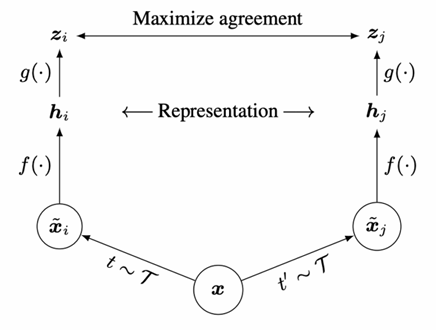
\includegraphics[width=0.5\linewidth]{chapters/unlabeled/simclr.png}
    \caption{Схематичное представление алгоритма SimCLR}
    \label{fig:enter-label-1}
\end{figure}

На рисунке можем схематичное представление последовательности шагов алгоритма со следующими обозначениями:

\begin{quote}
$x$ - исходное изображение,

$t, t'$ - разные аугментации на исходное изображение $x$ для получения представлений $\tilde{x_i}$, $\tilde{x_j}$,

$f$ - функция, генерирующая представления (representation) $h_i$, $h_j$ в виде вектора для входных изображений,

$g$ - функция, которая переводит вектора $h_i$, $h_j$ в величины $z_i$, $z_j$, для которых минимизируется расстояние (maximize agreement) в процессе обучения для аугментаций одного изображения и максимизируется для разных изображений.
\end{quote}

Шаги в обучении следующие:

1. К исходному изображению $x$ применяются аугментации $t, t'$. \textit{Аугментация} - это процесс создания новых данных на основе существующих с помощью преобразований. Такими преобразованиями для изображений являются, например, поворот, изменение яркости, гауссовское размытие и так далее. Она необходима, чтобы в новом признаковом пространстве изменённые изображения так же находились близко к изображениям того же класса.

2. К аугментированным изображениям $\tilde{x_i}$, $\tilde{x_j}$ применяется функция $f$, генерирующая векторное представление этих изображений $h_i$, $h_j$.

3. К векторным представлениям $h_i$, $h_j$ применяется функция $g$ для перевода в другое векторное представление. Данный шаг необязательный для обучения методом SimCLR.

4. Для $z_i$, $z_j$ уменьшается расстояние, если $\tilde{x_i}$, $\tilde{x_j}$ - аугментации одного и того же изображения, и увеличивается - если разных. Происходит это путём минимизации контрастивной функции потерь. 

Таким образом мы находим новое признаковое описание для изображения, с помощью которого можно обучиться на задачу классификации изображений, то есть найти функция $c$ из раздела про Суперпозицию.

\section{Вопросы}
\hspace{2em}1. Что такое суперпозиция в контексте построения модели для неразмеченных данных, и как она помогает в решении задачи с использованием методов глубокого обучения?

2. Каковы основные этапы и задачи в методе SimCLR?

3. Как аугментация данных способствует улучшению качества обучаемых представлений?


    \clearpage
    \chapter{Квазилинейные классификаторы}
    \section{Квазилинейные композиции}

Линейные корректирующие операции естественным образом обобщаются на тот случай, когда веса базовых алгоритмов не постоянны и зависят от положения объекта $x$ в пространстве $X$.

Поставим каждому базовому алгоритму $b_{t}(x)$ в соответствие функцию компетентности $g_{t}(x)$, принимающую значения из отрезка [0, 1]. Определим композицию так, чтобы ответ базового алгоритма $b_{t}(x)$ на объекте $x$ учитывался с весом $g_{t}(x)$.

\textbf{Определение.} Квазилинейная корректирующая операция есть функция $F: \mathbb{R}^{2T} \rightarrow \mathbb{R}$:

\begin{equation}
    F(b_{1}, \dots, b_{T}, g_{1}, \dots, g_{T}) = \sum_{t=1}^{T}g_{t} b_{t}.
    \label{main_eq}
\end{equation}

Соответственно, алгоритмическая композиция имеет вид:

\begin{equation*}
    a(x) = C(\sum_{t=1}^{T}g_{t}(x)b_{t}(x)),
\end{equation*}

где $C$ - фиксированное решающее правило. Чем больше значение $g_{t}(x)$, тем с большим весом учитывается ответ алгоритма $b_{t}(x)$ на объекте $x$. Множество:

\begin{equation*}
    \Omega_{t} = \{x\in X: g_{t}(x) > g_{s}(x), s = 1, \dots, T, s \neqt\}
\end{equation*}

называется областью компетентности базового алгоритма $b_{t}(x)$.

Основная идея смесей заключается в применении принципа «разделяй и властвуй». Используя достаточно простые базовые алгоритмы $b_{t}(x)$ и функции компетентности $g_{t}(x)$, можно восстанавливать довольно сложные зависимости.

Понятие области компетентности было введено Растригиным в \cite{растригин1981коллективные}. В англоязычной литературе композиции вида (\ref{main_eq}) принято называть смесями экспертов
(mixture of experts, ME), базовые алгоритмы — экспертами, функции компетентности — шлюзами (gates) \cite{jacobs1991adaptive}. Шлюзы определяют, к каким экспертам должен быть
направлен объект x. По-русски «смесь экспертов» звучит не очень удачно, поэтому
будем говорить о «смесях алгоритмов». Произведения $g_{t}(x)b_{t}(x)$ называются компонентами смеси.

Естественным требованием к шлюзам является условие нормировки:

\begin{equation}
    \sum_{t=1}^{T}g_{t}(x) = 1, \forall x \in X.
    \label{norm}
\end{equation}

Если оно выполнено, то для любого объекта x коррекция сводится к усреднению ответов базовых алгоритмов с некоторыми весами, причём результат никогда
не выходит за пределы отрезка $[\min_{t}b_{t}(x), \max_{t}b_{t}(x)]$.

Чтобы гарантировать выполнение условия нормировки (\ref{norm}), используют функцию «мягкого максимума» SoftMax: $\mathbb{R}^{T} \rightarrow \mathbb{R}^{T}$:

\begin{equation*}
    \widetilde{g}_{t} (x) = SoftMax_{t}(g_{1}(x), \dots, g_{T}(x)) = \dfrac{e^{\beta g_{t}(x)}}{e^{\beta g_{1}(x)} + \cdot + e^{\beta g_{T}(x)}} .
\end{equation*}


Эта функция переводит вектор $(g_{1}, \dots, g_{T})$ в нормированный вектор $(\widetilde{g}_{1}, \dots, \widetilde{g}_{T})$.
При $\beta \rightarrow \infty$, все компоненты $\widetilde{g}_{t}$ стремятся к нулю, кроме одной, соответствующей максимальному значению $\max_{t} g_{t}$, которая стремится к единице. Чем больше значение параметра $\beta$, тем «чётче» границы областей компетентности.

В задачах классификации с пороговым решающим правилом $C(b) = [b > 0]$ или $C(b) = sign(b)$ делать нормировку, вообще говоря, не обязательно, поскольку для классификации важен только знак выражения (\ref{main_eq}).

\subsection{Задача обнаружения нетипичных объектов}

 Если значение $g_{t}(x)$ меньше некоторого порога для всех $t = 1,\dots,T$, то можно полагать, что объект x попадает в «область неуверенности», где все алгоритмы не компетентны. Как правило, это связано с тем, что в данной области обучающих прецедентов просто не было. Таким образом, смеси алгоритмов позволяют решать задачу обнаружения нетипичных объектов или новизны (novelty detection). Иногда эту задачу называют классификацией с одним классом (one-class classification).

 \subsection{Вероятностная интерпретация}
 
Функции $g_{t}(x)$ можно интерпретировать как
нечёткие множества, а при условии нормировки — и как вероятностные распределения. Если для байесовского классификатора расписать апостериорные вероятности
классов, то функции компетентности приобретут смысл априорных вероятностей:

\begin{equation*}
    a(x) = arg_{y\in Y} max \lambda_{y} P\{y|x\} = arg_{y\in Y} max \lambda_{y} \sum_{t=1}^{T} \underbrace{P(t)}_{g_{t}(x)} \underbrace{P\{y|t, x\}}_{b_{t_{y}}(x)}.
\end{equation*}

Здесь предполагается, что каждый базовый алгоритм $b_{t}(x)$ возвращает вектор апостериорных вероятностей $(P\{y|t, x\})_{y\in Y}$. Затем квазилинейная корректирующая операция переводит T таких векторов в один вектор апостериорных вероятностей $(P\{y| x\})_{y\in Y}$, и к нему применяется решающее правило $arg\:max_{y}$.


Вероятностная интерпретация приводит к ЕМ-алгоритму, который обрастает массой технических усложнений. Мы рассмотрим более простые оптимизационные методы, основанные на применении выпуклых функций потерь.

\subsection{Вид функций компетентности}


Вид функций компетентности определяется спецификой предметной области. Например, может иметься априорная информация о том, что при больших и малых значениях некоторого признака f(x) поведение целевой зависимости принципиально различно. Тогда имеет смысл использовать весовую функцию вида:

\begin{equation*}
    g(x;\alpha, \beta) = \sigma(\alpha f(x) + \beta),
\end{equation*}

где $\alpha, \beta \in \mathbb{R}$ - свободные параметры, $\sigma(z) = (1 + e^{-z})^{-1}$ - сигмоидная функция позволяющая описать плавный переход между двумя областями компетентности.


Если априорной информации нет, то в качестве «универсальных» областей компетентности берут области простой формы. Например, в пространстве $X = \mathbb{R}^{n}$ можно взять полуплоскости:

\begin{equation*}
    g(x;\alpha, \beta) = \sigma(x^{T}\alpha + \beta),
\end{equation*}


или сферические гауссианы:

\begin{equation*}
    g(x;\alpha, \beta) = e^{-\beta ||x - \alpha ||^{2}},
\end{equation*}


 где $\alpha \in \mathbb{R}^{n}$, $\beta \in \mathbb{R}$ — свободные параметры, которые настраиваются по выборке аналогично тому, как настраиваются параметры базовых алгоритмов.
\subsection{Выпуклые функции потерь}

Преимущество смесей в том, что они позволяют разбить всё пространство X на области, в каждой из которых задача решается относительно просто, и затем «склеить» эти решения в единую композицию. Основной технический приём, позволяющий решить эти относительно простые подзадачи по-отдельности, независимо друг от друга, связан с использованием выпуклых функций потерь. Рассмотрим функционал, характеризующий качество алгоритмических операторов при заданном векторе весов объектов $W^{l} = (w_{l}, \dots , w_{l})$.

\textbf{Гипотеза.} Функция потерь $\widetilde{L}(b, y)$ является выпуклой по b, то есть для любых
$b_{1}, b_{2} \in \mathbb{R}$, $y \in Y$ и неотрицательных $g_{1},\;g_{2}$, таких, что $g_{1} + g_{2} = 1$, выполняется:

\begin{equation*}
    \widetilde{L}(g_{1}b_{1} + g_{2}b_{2}, y) \leq g_{1} \widetilde{L}(b_{1}, y) + g_{2} \widetilde{L}(b_{2}, y).
\end{equation*}

Условие выпуклости имеет прозрачную интерпретацию: потери растут не медленнее, чем величина отклонения от правильного ответа y. Во многих задачах требование выпуклости является естественным. В частности, ему удовлетворяет квадратичная функция $\widetilde{L}(b, y) = (b−y)^{2}$, применяемая в регрессионных задачах. К сожалению, пороговая функция $\widetilde{L}(b, y) = [by < 0]$, применяемая в задачах классификации при $Y = \{-1, +1\}$, не является выпуклой. Однако некоторые её непрерывные аппроксимации выпуклы:

\begin{equation*}
    \widetilde{L}(b, y) = [by < 0] \leq 
    \begin{cases}
        e^{-by} &- \text{экспоненциальная (AdaBoost);} \\
        log_{2}(1 + e^{-by})&- \text{логарифмическая (LR);}\\
        (1-by)_{+}&- \text{кусочно-линейная (SVM).}
    \end{cases}
\end{equation*}

Замена пороговой функции потерь на непрерывную является распространённой практикой. В частности, логарифмическая аппроксимация используется в логистической регрессии , экспоненциальная — в алгоритме AdaBoost , кусочно-линейная — в методе опорных векторов SVM . Непрерывные функции потерь имеют важное достоинство — они штрафуют обучающие объекты за приближение к границе классов, что способствует увеличению зазора между классами и повышению надёжности классификации. Таким образом, требование выпуклости функции потерь не слишком обременительно и даже естественно как для задач регрессии, так и для классификации.

Итак, пусть выполнено условие нормировки (\ref{norm}) и функция потерь $\widetilde{L}$ выпукла. Вместо функционала Q(a) будем минимизировать его верхнюю оценку, которая непосредственно вытекает из условия выпуклости:

\begin{equation}
    Q(a) = \sum_{i=1}^{l} \widetilde{L}(\sum_{t=1}^{T} g_{t}(x_{i})b_{t}(x_{i}), y_{i}) \leq \sum_{i=1}^{l}\underbrace{\sum_{t=1}^{T} g_{t}(x_{i}) \widetilde{L}(b_{t}(x_{i}), y_{i})}_{Q(b_{t},W^{l})}.
    \label{qa}
\end{equation}


Функционал Q(a) распадается на сумму T функционалов, каждый из которых зависит только от $b_{t}$ и $g_{t}$. Если зафиксировать функции компетентности $g_{t}$, то все базовые алгоритмы $b_{t}$ можно настроить по-отдельности, независимо друг от друга. Это стандартная задача обучения базовых алгоритмов. Затем можно зафиксировать базовые алгоритмы и настроить их функции компетентности. Для настройки всей композиции организуется итерационный процесс, в котором эти два шага выполняются по очереди. Остаётся только понять, каким образом компоненты будут добавляться в смесь, как строить для них начальные приближения, и когда прекращать порождение новых компонент.


 \subsection*{Задачи}
 \begin{enumerate}
     \item Исследовать на выпуклость функции потерь:
     \begin{enumerate}
         \item $\widetilde{L}(M) = (1 - M)^{2}$ - квадратичная функция потерь,
         \item $\widetilde{L}(M) = 2(1 + e^{M})^{-1}$ - сигмоидная функция потерь.
     \end{enumerate}
     %\item Почему функция $SoftMax$ нельзя заменить простой нормировкой вида:
     %\begin{equation*}
     %    \widetilde{g}_{t}(x) = \dfrac{g_{t}(x)}{\sum_{i = 1}^{T}g_{t}(x)}.
     %\end{equation*}
     \item Дана задача линейной регрессии для пары экспертов. Пусть выбраны функции компетентности сигмоидного типа с $n = 1$, $\beta_{1, 2} = 0$, $\alpha_{1} = 0,14$ и $\alpha_{2} = 3,14$. Определить предсказание "двух экспертов" в точке 0,5 , если эксперты имеют вид $\mathcal{N}_{1}$(0, 2) и $\mathcal{N}_{2}$(1, 1).

     \item Дано: два решающих пня с порогами 5 и 10, веса объектов одинаковы и равны 0,1 . Найти функции компетентности для данных решающих пней из функций вида:
     \begin{equation*}
         g(x;\alpha, \beta) = e^{-\beta (x - \alpha)^{2}}.
     \end{equation*}

     Данные для задачи:
     \begin{table*}[h]
     \centering
\begin{tabular}{|c|c|c|}
\hline
 i&         x_{i}     &    y_{i}         \\ \hline
0 & 0,744  & \cellcolor[HTML]{3166FF}-1 \\ \hline
1 & 1,619  & \cellcolor[HTML]{3166FF}-1 \\ \hline
2 & 4,694  & \cellcolor[HTML]{3166FF}-1 \\ \hline
3 & 4,882  & \cellcolor[HTML]{FE0000}+1  \\ \hline
4 & 6,08   & \cellcolor[HTML]{3166FF}-1 \\ \hline
5 & 8,726  & \cellcolor[HTML]{FE0000}+1  \\ \hline
6 & 10,753 & \cellcolor[HTML]{FE0000}+1  \\ \hline
7 & 11,754 & \cellcolor[HTML]{3166FF}-1 \\ \hline
8 & 18,349 & \cellcolor[HTML]{FE0000}+1  \\ \hline
9 & 18,669 & \cellcolor[HTML]{FE0000}+1  \\ \hline
\end{tabular}
\end{table*}
 \end{enumerate}

 \subsection*{Ответы к задачам}
 \begin{enumerate}
    \item (a) - выпуклая, (b) - невыпуклая.
    \item (В работе).
    \item (В работе)
 \end{enumerate}


    \clearpage
    \chapter{Детекция аномалий}
    \section{Open-Set Recognition}

Open-Set Recognition - метод распознавания с открытым набором параметров.
Порой может случиться так, что тестовый пример может быть визуально или метрически очень похожим на одну из категорий.
Наша задача - понять, когда эта кластеризация корректна, а когда мы делаем поспешные выводы.

\subsection{Основная идея}
Главной целью является попытка отличить похожие категории, которые были распознаны во время обучения, от новых, не идентифицированных. 
Другими словами, OSR специализируется на выявлении семантических сдвигов между категориями при обучении и тестировании.
Мотивацию можно представить как желание попытаться исключить ошибочное распознавание при близких параметрах, так как в реальном мире модели должны уметь не только различать объекты на существующих классах, но и идентифицировать случаи, когда сэмпл пришел из класса, который еще не встречался ранее.
Более инуитивное представление поможет получить картинка \ref{fig:anomalies-abstract}.

\begin{figure}[ht]
	\centering
	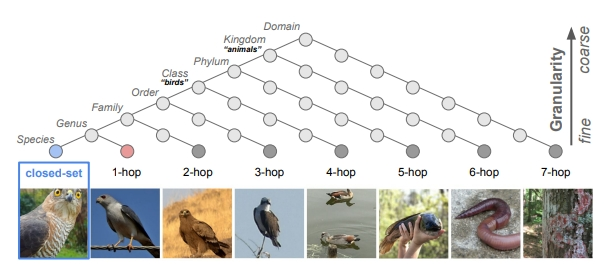
\includegraphics[width=0.8\linewidth]{chapters/anomalies/images/anomalies-abstract.jpg}
	\caption{Пример близких категорий из биологии}
	\label{fig:anomalies-abstract}
\end{figure}

На картинке мы видим, что чем дальше друг от друга виды животных на основе визуального восприятия, тем проще утверждать, что они относятся к разным классам и имеют более далеких предков.
Но чем ближе (пример - птицы), тем все труднее говорить о схожести видов, что может стать большой проблемой в силу некорректного отнесения животных к одному классу, роду или виду.
Иногда данная задача вызывает проблемы даже при попытке проделать ее самостоятельно, визуально.

\subsection{Постановка задачи}
Пусть у нас есть простанство объектов $X$, множество уже известных классов $Y = \{y_1, \dots, y_n\}$ и класс $u$ неизвестности, с которым мы как раз и должны научиться работать.

Модель в идеале должна сделать одно из двух следующих действий:
\begin{enumerate}
    \item Присвоить объекту $x \in X$ метку $y \in Y$, если объект принадлежит одному из известных классов.
    \item Присвоить метку $u$, если он не относится ни к одному из классов.
\end{enumerate}

\subsection{Методы}
\begin{enumerate}
    \item \textbf{На основе порога уверенности}
    
    Возьмем $S(x)$ за функцию, обозначающую отклик модели, он должен расти по мере роста $\mathcal{P}(y \in Y | x)$, где $y$ - предполагаемый класс объекта $x$. 
    Тогда:
    \begin{itemize} 
        \item Если $\max\limits_{y \in Y}{\mathcal{P}(y|x)}$ больше заранее определенного порога $\varepsilon$, то объект классифицируется моделью как принадлежащий $\hat{y} = \arg\max\limits_{y \in Y}{\mathcal{P}(y|x)}$.
        \item Если же меньше, то как неизвестный: $\hat{y} = u$
    \end{itemize}

    \item \textbf{На основе расстояний}
    
    Данный метод подходит если мы можем определить какую-либо метриуц на объектах.
    Метод основан на вычислении растояния от объекта до центров уже известных классов.
    
    Обозначим центры уже известных классов за $c_1, \dots, c_n$. 
    Обозначим за расстояние до центра $i$ за $d(x, c_i) = || x - c_i ||$. 
    Тогда:
    \begin{itemize}
        \item Если расстояние до ближайшего центра $cl(x) = \min\limits_{i}d(x, c_i)$ меньше заранее фиксированного порога $\varepsilon$, то объект классифицируется как принадлежащий $\hat{y} = \arg\min\limits_{i}d(x, c_i)$.
        \item Иначе же - как неизвестный: $y = u$.
    \end{itemize}
\end{enumerate}

По сути мы хотим минимизировать как количество ошибок классификации принадлежания одному из уже известных классов, так и отнесения к неизвестным объектам.
Стоит отметить, что при наличии явных выбросов или объектов, сильно отстояших от классов модель ложно отнесет их к неизвестным.

\subsection{Применение}
\begin{itemize}
    \item \textbf{Медицина}: распознавание и диагностика заболеваний, которые ранее могли быть еще не изучены или не встречаться
    \item \textbf{Биология}: пример с видами животных
    \item \textbf{Биометрия}: наверное самый наглядный пример, распознавание лица или отпечатка пальца человека. Мы должны сказать, является ли он известным или кто-то пытается взломать наш телефон
\end{itemize}

\subsection{Задачи}
Попробуйте ответить на следующие вопросы:

\problem Рассмотрим, как размер обучающей выборки для $n$ классов влияет на результат работы модели Open-Set Recognition. 
Формализуйте, как увеличение числа объектов в обучающей выборке может повлиять на вероятность ложных срабатываний и пропусков для неизвестных объектов.
\solution При небольшом размере обучающей выборки у модели не будет достаточной информации для точного определения границ между классами, что может привести к более высокому числу как ложных классификаций, так и ложных отнесений к неизвестному классу в силу отсутствия у нее возможности корректно научиться определять границы.

\problem Предложите метрику или способ обучения, которые вы бы использовали для оценки точности модели.
\solution С ходу понятно, как определять, что модель дала верный или не верный результат по уже известному классу. 
Но основная проблема состоит в том, чтобы оценить ее работу на объектах из неизвестного класса.
Давайте уберем из набора данных, используемого для тренировки часть, связанную с какими-либо известными классами, близкими к другим и будем валидировать способность нашей модели выделять неизвестные классы на ней.
Для оценки качества модели мы сможем применить метрику точности, равную отношению количества верных предсказаний в обоих случаях к общему количеству объектов:
$$Accuracy = \frac{TP + TR}{TP + TR + FP + FR},$$
где:
\begin{itemize}
    \item $TP$ - количество верных классификаций к одному из известных
    \item $TR$ - количество верных отнесений к неизвестному классу
    \item $FP$ - количество ошибочных кассификаций объекта как известного
    \item $FR$ - количество ошибочных отнесений объекта к неизвестным
\end{itemize}

\problem Предложите алгоритм, который можно было бы легко применить к задаче Open-Set Recognition.
\solution Давайте модифицируем логистическую регрессию. Для каждого класса $y_i$ она генерирует вероятность $\mathcal{P}(y_i|x)$, вычисляемую через сигмоидальную функцию.
Затем применим метод, основанный на пороге уверенности.

\section{Теория робастного (помехоустойчивого) обучения}
Традиционные методы обучения основываются на
том, что тренировочная выборка хорошо препроцессирована и не содержит шумов,
выбросов и недостающих значений. В реальных условиях хорошо структурировать
выборку не всегда возможно. В таких случаях на помощь могут прийти методы
робастного обучения.

Робастное обучение - это подход, фокусирующийся на построении моделей,
сохраняющих точность на неидеальных данных. Такая устойчивость обеспечивается
адаптивным подходам к входным данным. Методы обастного обучение частно
используют альтернативные функции потерь, алгоритмов, адаптирующихся к
структурам данных и/или детектирование и соответсвующую обработку аномалий.

\subsection{Схема итерационного взвешивания (IRS)}
IRS (Iterative Reweighting Scheme) - это один из
методов робасного обучения, заключающийся в обновлении весов объектов на каждом
шаге. Это позволяет уменьшить влияние аномальных данных. Вместо традиционных
функций потерь (таких как среднеквадратичная ошибка) в итерационной схеме
используются взвешенные функции потерь. IRS работает по следующему алгоритму:

\begin{enumerate}
  \item Инициализация весов
    Начинаем с иницаиализации весов:
    \[w_i^{(0)} = \frac{1}{l}, \forall i = 1, ..., l\]
  \item Обновление модели
    \[\alpha := arg min_{\alpha} \sum_{i=1}^l w_i L_i\left(\alpha\right) + \tau R\left(\alpha\right)\]

    \[w_i = norm_i\left( \mu^{'}\left( L_i(\alpha) \right) \right), i = 1, ..., l\]

    \[norm_i(v_i) = \frac{v_i}{\sum_j v_j}\]
  \item Повторяем обновление модели пока веса не стабилизируются или пока не
    будет достигнуто заданное число шагов
\end{enumerate}

\subsection{Задачи}
\subsubsection{Задача 1}
Предположим, что вы применили итеративную схему перевзвешивания на наборе
данных, содержащем выбросы. Вы применяете схему итеративного взвешивания.
По каким параметрам вы поймёте, чтоалгоритм сошёлся?
\textit{Ответ}: Веса изменяются не сильно, функция потерь перестала существенно
изменяться.
\subsubsection{Задача 2}
Предположим, что вы применили схему итерационного перевзвешивания к набору
данных и получили следующие веса на трех итерациях:
\[ w(1) = [0.40, 0.30, 0.20, 0.10] \]
\[ w(2) = [0.45, 0.25, 0.20 ,0.10] \]
\[ w(3) = [0.43, 0.26, 0.20, 0.10] \]

Считая критерием сходимости изменение весов и порог \(\epsilon = 0.01\),
скажите, сошёлся ли алгоритм/
\textit{Ответ}:
\[ \Delta w^{1\rightarrow2} = max\left( \abs{0.4-0.45}, \abs{0.3 - 0.25}, \abs{0.2-0.2}, \abs{0.1-0.1}  \right) = 0.05 \]
\[ \Delta w^{2\rightarrow3} = max\left( \abs{0.43-0.45}, \abs{0.26 - 0.25}, \abs{0.2-0.2}, \abs{0.1-0.1}  \right) = 0.02 \]
Т.к. обе дельты больше \(\epsilon\), то алгоритм не сошёлся.

\subsubsection{Задача 3}
Хоошо ли работают алгоритмы итеративного перевзвешивания на данных с высокой
мультиколлинеарностью?
\textit{Ответ}: Работает плохо, т.к. в алгоритме перевзвешивания веса объектов
обновляются независимо, а значит, изменение веса одного объекта не влияет на
вес второго. В случае высокой зависимости между данными этот подход не может
быть применён, т.к. они требуют согласованного изменения весов кореллирующих
объектов.





    % Bibliography
    \clearpage
    \printbibliography
\end{document}
